\documentclass[11pt,a4paper,english,greek,twoside]{hsis-thesis}
%\DeclareGraphicsRule{.tif}{bmp}{}{}

\usepackage[export]{adjustbox}
\usepackage{afterpage} % commands can be expanded after the curent page
\usepackage{algorithm}
\usepackage{algpseudocode}
%\usepackage{algorithmic}
%\usepackage{algorithmicx}
%\usepackage{algcompatible}
\usepackage{amsmath} % improving the information structure and printed output
\usepackage{amssymb} % an extended symbol collection
\usepackage{amsthm} % helps to define theorem-like structures
\usepackage{array} % options for column formats
\usepackage{babel} % culturally-determined typographical rules
%\usepackage[english,greek]{babel}
\usepackage[unicode]{hyperref}
\hypersetup{
    unicode=true,       % non-Latin characters in Acrobat’s bookmarks
    pdftitle={Τεχνικές Ανοχής Ελαττωμάτων Σε Μηχανισμούς Πρόβλεψης Εντολών Αλλαγής Της Ροής Του Προγράμματος}, % title
    pdfauthor={Φιλίππου Φίλιππος},     % author
    pdfsubject={Διπλωματική Εργασία},  % subject of the document
    pdfcreator={TeXstudio},            % creator of the document
    %pdfkeywords={Fault Tolerance, Dynamic Voltage and Frequency Scaling, Ultra-Low Supply Voltage, Branch Prediction, Branch Target Buffer}, % list of keywords
    pdfkeywords={Ανοχή Σφαλμάτων, Δυναμική Μεταβολή Τάσης και Συχνότητας, Πολύ-Χαμηλή Τάση Λειτουργίας, Πρόβλεψη Διακλάδωσης, Πίνακας Πρόβλεψης Προορισμού Διακλάδωσης}, % list of keywords
    pdfnewwindow=true,  % links in new window
    colorlinks=true,    % false: boxed links; true: colored links
    linkcolor=black,    % color of internal links
    citecolor=black,    % color of links to bibliography
    filecolor=black,    % color of file links
    urlcolor=black      % color of external links
}
\usepackage{bookmark} % new bookmark organization for package hyperref
\usepackage{booktabs} % enhance the quality of tables
\usepackage{caption} % customised captions
\usepackage{cmap}  % makes PDF files "searchable and copyable" in acrobat reader
\usepackage{datetime} % different formats for displaying the current time
\usepackage{enumitem} % control of list environments: enumerate, itemize and description
\usepackage{epsfig} %solution to the problem of including graphicsof including graphics
\usepackage{epstopdf} % converts the input PostScript file to PDF
\usepackage{etoolbox} % toolbox of programming tools (maybe for \AtBeginEnvironment)
\usepackage{float} % define floating objects
\usepackage[T1]{fontenc}
\usepackage{graphicx} % extended graphics package
\usepackage{indentfirst} % the first line of all sections gets a paragraph indentation
\usepackage{index} % better and more robust support for indexes
%\usepackage[utf8]{inputenc}
%\usepackage[iso-8859-7]{inputenc}
\usepackage{latexsym} % additional characters available from the lasy fonts
\usepackage{makecell} % create common layout for tabular material
%\usepackage{makeidx} % \see and \printindex commands
\usepackage{multirow} % table cells that span more than one row of the table
\usepackage{ragged2e} % for smart ragged align in last column
\usepackage{subcaption} % typesetting of sub-captions
\usepackage{tabularx} % modifies the widths of certain columns
%\usepackage{textgreek}
\usepackage{tcolorbox} % colored and framed text boxes with a heading line
%\usepackage{tocloft} % typographic design of the ToC, LoF and LoT
\usepackage{textcomp} % text symbols in the TS1 encoding
\usepackage[explicit]{titlesec} % commands for selection from various title styles
\usepackage{tocbibind} % add document elements to the Table of Contents
\usepackage{url} % formatting email, links, paths, etc.
\usepackage{verbatim} % reimplements the verbatim and verbatim* environments
\usepackage{xspace} % adds a space after a text macro

\usepackage{mathtools}
\DeclarePairedDelimiter\ceil{\lceil}{\rceil}
\DeclarePairedDelimiter\floor{\lfloor}{\rfloor}
\newcommand\addtag{\refstepcounter{equation}\tag{\theequation}}

% page Layout: use it for debugging only
%\usepackage{showframe}

% display the links in the same style as the rest of the text
\urlstyle{same}

\def\tabularxcolumn#1{m{#1}} %vertical alignment center for tabularx columns

\newindex{default}{idx}{ind}{Ευρετήριο όρων}
\newindex{en}{edx}{end}{Ευρετήριο αγγλικών όρων}
%\makeindex

% Page definitions
%\setlength{\textheight}{23cm} \setlength{\textwidth}{15.5cm}
%\setlength{\oddsidemargin}{0.2cm}
%\setlength{\evensidemargin}{0.2cm} \setlength{\topmargin}{-1.2cm}
%\setlength{\headsep}{1.5cm}

% define email address
\newcommand{\email}{\href{mailto:filippo@ceid.upatras.gr}{\nolinkurl{filippo@ceid.upatras.gr}}} 

% 1.5 spacing
\renewcommand{\baselinestretch}{1.2}

\newcommand\blankpage{
    \null
    \thispagestyle{empty}
    \addtocounter{page}{-1}
    \newpage
}

\newcommand*\Hide{
    \titleformat{\chapter}[display]
      {}{}{0pt}{\Huge}
    \titleformat{\part}
      {}{}{0pt}{}
}

% define language commands for small texts
\newcommand{\gr}[1]{\textgreek{#1}}
\newcommand{\tl}[1]{\textlatin{#1}}
\newcommand{\en}[1]{\foreignlanguage{english}{#1}}

% define comment styles
\newcommand{\linecomment}[1]{\textit{// #1}}
\newcommand{\fullcomment}[1]{\textit{/* #1 */}}

% define math expressions
\newcommand{\set}[1]{\left\{#1\right\}}
\newcommand{\expnum}[1]{#1\mathrm{e}{-03}}
\newcommand{\nm}{\en{nm}\xspace}
\newcommand{\xor}{\textit{\en{XOR}}\xspace}
\newcommand{\mathgr}[1]{\textit{\textgreek{#1}}}

% define english acronyms
\newcommand{\ipc}{\en{IPC}\xspace}
\newcommand{\edp}{\en{EDP}\xspace}

% define used programs
\newcommand{\gem}{\en{gem5}\xspace}
\newcommand{\mcpat}{\en{McPAT}\xspace}
\newcommand{\cacti}{\en{CACTI}\xspace}
\newcommand{\matlab}{\en{MATLAB}\xspace}
\newcommand{\matlabR}{\en{MATLAB}\SymbR\xspace}
\newcommand{\spec}{\en{SPEC CPU2006}\xspace}

% define subfolders here
\newcommand{\algorithmsDIR}{algorithm_examples}
\newcommand{\hardwareDIR}{hardware_figures}
\newcommand{\resultsDIR}{results_charts}
\newcommand{\simulationsDIR}{simulation_outputs}
\newcommand{\researchesDIR}{other_researches}

% define glossary format
\newcommand{\gloss}[2]{#1 \> \en{#2}\\ }

% define greek names for captions
\captionsetup[table]{name=\gr{Πίνακας}}
\captionsetup[algorithm]{name=\gr{Αλγόριθμος}}
\captionsetup[figure]{name=\gr{Σχήμα}}
\captionsetup[subfigure]{subrefformat=simple,labelformat=simple}
\renewcommand\thesubfigure{(\alph{subfigure})}

% change the algorithm naming to greek "Αλγόριθμος"
\makeatletter
\renewcommand{\ALG@name}{\gr{Αλγόριθμος}}
\makeatother

% define new algorithm comment style
\algrenewcommand{\algorithmiccomment}[1]{/* #1 */}

% remove "anw tonos” in the greek alphabetical numerals
\makeatletter
\let\anw@true\anw@false
\makeatother

\bibliographystyle{ieeetr}

\selectlanguage{greek}
%\hyphenation{τμή-μα Επο-μέ-νως}

\begin{document}
    \selectlanguage{greek}
    \maketitle
    \frontmatter
    \pagenumbering{roman}
    \mainmatter
    
    \begin{acknowledgements}
    Με την περάτωση της διπλωματικής μου εργασίας και την ολοκλήρωση των μεταπτυχιακών σπουδών μου θα ήθελα να ευχαριστήσω όλους όσους με στήριξαν κατά την περίοδο φοίτησής μου και με βοήθησαν με το δικό τους ξεχωριστό τρόπο να διευρύνω τους ορίζοντες μου.
    
    Πρώτα απ' όλα αξίζουν ιδιαίτερες ευχαριστίες στον επιβλέποντα καθηγητή μου κ. Δημήτρη Νικολό, ο οποίος μου έδωσε την ευκαιρία να ασχοληθώ με το κομμάτι της ερευνάς και για πρώτη φορά να παραστώ ως ομιλητής σε επιστημονικό συνέδριο.
    
    Επίσης ευχαριστώ θερμά τον συνεπιβλέποντά μου κ. Γιώργο Κεραμίδα για όλη την πολύτιμη υποστήριξη που μου πρόσφερε από τις προπτυχιακές κιόλας σπουδές μου έως σήμερα. Φυσικά να μην παραλείψω τον υποψήφιο διδάκτορα κ. Μιχάλη Μαυρόπουλο για την βοήθειά που μου προσέφερε κατά την περίοδο της ενασχόλησής μου στην έρευνα, μέσω της άριστης συνεργασίας μας.
    
    Τέλος και πάνω απ' όλα, ευχαριστώ την οικογένειά μου που με την οικονομική και ψυχολογική υποστήριξή τους, μου πρόσφεραν τη δυνατότητα να παρακολουθήσω ένα πλούσιο πρόγραμμα σπουδών και να προετοιμαστώ καταλλήλως για την επαγγελματική ενασχόληση μου στον τομέα των νέων τεχνολογιών.
\end{acknowledgements}

%----------------------------------------------------------%
\begin{abstract}
    \vspace{-3ex}
    Η τεχνική της μείωσης της τάσης τροφοδοσίας, που χρησιμοποιείται για τη μείωση της κατανάλωσης ισχύος, αυξάνει την ευαισθησία των κυκλωμάτων στις αποκλίσεις των παραμέτρων τους από τις ονομαστικές τιμές και οδηγεί στην εκθετική αύξηση του πλήθους των δυσλειτουργικών κυψελίδων. Η παρούσα διπλωματική εργασία, επικεντρώνεται στη μελέτη της συμπεριφοράς του μηχανισμού πρόβλεψης εντολών αλλαγής της ροής του προγράμματος (εντολές διακλάδωσης),όταν τα στοιχεία που τον αποτελούν εμφανίζουν σφάλματα εξαιτίας δυσλειτουργικών κυψελίδων.
    
    Παρότι ελαττώματα στο μηχανισμό πρόβλεψης εντολών διακλάδωσης δεν εμποδίζουν την ορθή εκτέλεση των προγραμμάτων, όπως αναδεικνύεται στην παρούσα εργασία, η εμφάνιση σφαλμάτων στις κυψελίδες μνήμης του Πίνακα Πρόβλεψης Προορισμού Διακλάδωσης, ο οποίος αποτελεί τμήμα του μηχανισμού πρόβλεψης, μπορεί να έχει σημαντικές επιπτώσεις στην απόδοση και την κατανάλωση ενέργειας κατά την εκτέλεση ενός προγράμματος. Στην παρούσα εργασία, πραγματοποιείται εξονυχιστική μελέτη της λειτουργίας του Πίνακα Πρόβλεψης Προορισμού Διακλάδωσης και της επίδρασης των σφαλμάτων του στην απόδοση και την κατανάλωση ισχύος, για διαφορετικά πλήθη σφαλμάτων και παραμετροποιήσεις του συστήματος. Αντιθέτως, όπως αποδεικνύεται, σφάλματα στα στοιχεία του Πίνακα Πρόβλεψης Διακλάδωσης, τα οποία αποτελούν το υπόλοιπο τμήμα του μηχανισμού, έχουν αμελητέα επίπτωση στην απόδοση και συνεπώς στη συνολική κατανάλωση ενέργειας.
    
    Για τη μείωση των επιπτώσεων που έχει η δυσλειτουργία των κελιών μνήμης του Πίνακα Πρόβλεψης Προορισμού Διακλάδωσης, παρουσιάζεται, για πρώτη φορά, ένας μηχανισμός αποφυγής της μείωσης της απόδοσης και της αύξησης της συνολικής κατανάλωσης ισχύος. Ο προτεινόμενος μηχανισμός απαιτεί ελάχιστη αύξηση σε υλικό και σχεδόν μηδενική καθυστέρηση. Επιπλέον, συνοδεύεται από κατάλληλο αλγόριθμο ώστε να επιτυγχάνεται προσαρμοστικότητα ανάλογα με το πλήθος των σφαλμάτων. Χρησιμοποιώντας τον εξομοιωτή \gem, τα μετροπρογράμματα \spec, ένα πλήθος χαρτών σφαλμάτων, και για δύο πιθανότητες σφάλματος οι οποίες αντιστοιχούν σε δύο διαφορετικές τάσης λειτουργίας πολύ-χαμηλής κατανάλωσης, παρουσιάζεται η αποτελεσματικότητα του προτεινόμενου μηχανισμού από άποψη Εντολών ανά Κύκλο ρολογιού (\ipc) και Γινομένου Ενέργειας-Κατανάλωσης (\edp), συγκριτικά με την περίπτωση μη χρήσης του.
    
    \vspace{-2ex}
    \begin{keywords}
        Ανοχή Σφαλμάτων, Δυναμική Μεταβολή Τάσης και Συχνότητας, Πολύ-Χαμηλή Τάση Λειτουργίας, Πρόβλεψη Διακλάδωσης, Πίνακας Πρόβλεψης Προορισμού Διακλάδωσης.
    \end{keywords}
    \vspace{-4ex}
    
\end{abstract}

%----------------------------------------------------------%

\begin{abstracteng}
    \selectlanguage{english}
    
    Dynamic voltage and frequency scaling (DVFS) increases the impact of process variations on memory cells reliability resulting in an exponential ramp-up in the number of malfunctioning memory cells. Current work, investigates the behavior of branch prediction unit with faulty memory cells in its components.
    
    Although being an intrinsically fault-tolerant unit (i.e., it does not affect correctness of the system), as shown in this work, the existence of faulty memory cells in a Branch Target Buffer (BTB), which is one of the branch prediction components, can damage the performance and increase the energy consumed by the executing applications. Especially, a deep analysis of the BTB function and the effect of its faults, for several fault fault probabilities and system configurations, is performed. On the other side, as evidenced, the presence of faulty memory cells in Branch Prediction Buffer (BPB), which constitutes the rest of the branch prediction, has a negligible impact in performance, and hence in total energy consumption.
    
    To remedy the negative impact of malfunctioning BTB memory cells, for the first time, a performance recovery mechanism is introduced. The proposed mechanism has both minimal hardware overheads and practically-zero additional delays. In addition, it is accompanied by an appropriate algorithm to achieve adaptability in every case of faults. Using the simulator \gem, the \spec benchmarks, a plethora of fault maps, and for two fault probabilities that correspond to two different low power consumption modes, the effectiveness of the proposed mechanism in terms of Instructions of per Circle (\ipc) and Energy-Delay Product (\edp), compared to the case where no mechanism is used for this purpose.
    
    \begin{keywordseng}
        Fault Tolerance, Dynamic Voltage and Frequency Scaling, Ultra-Low Supply Voltage, Branch Prediction, Branch Target Buffer.
    \end{keywordseng}
    
    \selectlanguage{greek}
\end{abstracteng}

    
    \tableofcontents
    
    \listoffigures
    
    \listoftables
    
    \chapter{Εισαγωγή}
\label{chap1}

Η συνεχώς αυξανόμενη ανάγκη για συρρίκνωση της τεχνολογίας των σύγχρονων ολοκληρωμένων κυκλωμάτων, καθώς και η προσπάθεια μείωσης της απαιτούμενης ενέργειας με ταυτόχρονη αύξηση της απόδοσης, έχουν φέρει στην επιφάνεια το πολύ σημαντικό πρόβλημα των σφαλμάτων στα στοιχεία μνήμης. Τα σφάλματα ενός ψηφιακού κυκλώματος στην καλύτερη περίπτωση ενδέχεται να έχουν απλώς μία επίπτωση στην απόδοση του συστήματος. Στην χειρότερη περίπτωση όμως μπορούν να προκαλέσουν ακόμη και την εξαγωγή λανθασμένων αποτελεσμάτων, δίχως αυτό να γίνεται αντιληπτό άμεσα. Για το λόγο αυτό έχουν αναπτυχθεί πληθώρα τεχνικών τόσο για τη μείωση τους όσο και την ανοχή τους κατά το μέγιστο δυνατόν.

%----------------------------------------------------------%

\section{Αντικείμενο της Διπλωματικής}
\label{chap1_Object}

Στην παρούσα διπλωματική μελετούνται τα σφάλματα στη Μονάδα Δυναμικής Πρόβλεψης Διακλαδώσεων των σύγχρονων υπερβαθμωτών επεξεργαστών, και αναζητείται λύση για τα σφάλματα που εμφανίζονται στον Πίνακα Πρόβλεψης Προορισμού Διακλάδωσης. Συγκεκριμένα, όπως θα παρουσιαστεί στα ακόλουθα κεφάλαια, τα σφάλματα αυτού του πίνακα παρότι δεν επηρεάζουν το τελικό αποτέλεσμα της εκτέλεσης ενός προγράμματος, μπορούν να προκαλέσουν σε ορισμένες περιπτώσεις σημαντική αύξηση του απαιτούμενη χρόνου ολοκλήρωσης του. Η αύξηση του χρόνου συνεπάγεται τη μείωση της απόδοσης καθώς και την αύξηση της καταναλισκόμενης ενέργειας.
\par
Όπως φανερώνει η μελέτη στον Πίνακα Πρόβλεψης Προορισμού Διακλάδωσης, η πτώσης της απόδοσης εξαιτίας των σφαλμάτων οφείλεται στην ύπαρξη πλήρως ελαττωματικών συνόλων, δηλαδή συνόλων των οποίων όλα τα πλαίσια είναι ελαττωματικά, με αποτέλεσμα την αδυναμία αποθήκευσης έγκυρης πληροφορίας για ένα πλήθος εντολών διακλάδωσης. Παρότι οι περιπτώσεις τέτοιων συνόλων είναι περιορισμένες, η ύπαρξή τους μπορεί να προκαλέσει πολύ μεγάλη αύξηση του συνολικού απαιτούμενου χρόνου ενός προγράμματος, οδηγώντας με αυτό τον τρόπο σε αύξηση της καταναλισκόμενης ενέργειας. Η λύση στο πρόβλημα αυτό δίνεται από την προτεινόμενη τεχνική της λογικής μετάθεσης των πλαισίων που αποτελούν τον Πίνακα Πρόβλεψης Προορισμού Διακλάδωσης, η οποία επιτυγχάνεται με ελάχιστο κόστος.

\section{Συνεισφορά}
\label{chap1_Contribution}

\begin{enumerate}[itemsep=0.5pt]
    \item Μελετήθηκε η συμπεριφορά της Μονάδας Δυναμικής Πρόβλεψης Διακλαδώσεων κατά τη λειτουργία σε κατάσταση πολύ χαμηλής κατανάλωσης, στην οποία εμφανίζονται σφάλματα εξαιτίας των ελαττωματικών στοιχείων.
    \item Προτείνεται μία ελαχίστου κόστους τεχνική επίλυσης των επιπτώσεων των σφαλμάτων του Πίνακα Πρόβλεψης Προορισμού Διακλάδωσης.
    \item Παρουσιάζεται κατάλληλος αλγόριθμος υπολογισμού σε τρεις εκδοχές, ο οποίος έχει τη δυνατότητα να προσαρμόζεται στην κάθε περίπτωση σφαλμάτων.
    \item Αξιολογήθηκε η επιτυχία κάθε εκδοχής του αλγορίθμου στην επίτευξη του στόχου.
    \item Μελετήθηκε η βελτίωση που προσφέρει η προτεινόμενη τεχνική στην απόδοση και την κατανάλωση του συστήματος όταν λειτουργεί σε κατάσταση χαμηλής κατανάλωσης.
\end{enumerate}

Τμήμα της παρούσας μελέτης έχει εκδοθεί στην ερευνητική εργασία με τίτλο $``$\textit{\en{Recovery of Performance Degradation in Defective Branch Target Buffers}}$"$, η οποία παρουσιάστηκε στο 22\textsuperscript{ο} διεθνές συνέδριο \en{On-Line Testing and Robust System Design} \cite{filippou2016recovery}.

%----------------------------------------------------------%

\section{Οργάνωση του Τόμου}
\label{chap1_Organization}

Στο Κεφάλαιο \ref{chap2} παρουσιάζονται οι μονάδες που αποτελούν τον Υπερβαθμωτό Επεξεργαστή και γίνεται ιδιαίτερη αναφορά στη Μονάδα Δυναμικής Πρόβλεψης Διακλαδώσεων. Αναλύονται τα στοιχεία που την αποτελούν, ο τρόπος λειτουργίας της καθώς και η σημασία χρήσης της.
\par
Στο Κεφάλαιο \ref{chap3} γίνεται μία γενική περιγραφή της σύγχρονης τεχνολογίας και της κατανάλωσης ενέργειας των σύγχρονων ολοκληρωμένων. Επίσης παρουσιάζεται η εμφάνιση βλαβών στις κυψελίδες \en{SRAM} κατά την προσπάθεια μείωσης της τάσης λειτουργίας των κυκλωμάτων. Τα στοιχεία που παρουσιάζονται αποτελούν τμήματα ερευνών που έχουν δημοσιευτεί.
\par
Στο Κεφάλαιο \ref{chap4} μελετάται η συμπεριφορά της Μονάδας Δυναμικής Πρόβλεψης Διακλαδώσεων όταν το ολοκληρωμένο κύκλωμα λειτουργεί σε χαμηλό δυναμικό.
\par
Στο Κεφάλαιο \ref{chap5} γίνεται η παρουσίαση της προτεινόμενης τεχνικής ανοχής σφαλμάτων, καθώς και του απαιτούμενου αλγορίθμου ώστε η τεχνική να είναι εφαρμόσιμη σε οποιοδήποτε ολοκληρωμένο διαθέτει τεχνική ανίχνευσης λαθών.
\par
Στο Κεφάλαιο \ref{chap6} παρουσιάζονται αναλυτικά τα αποτελέσματα εξομοιώσεων της προτεινόμενης τεχνικής σε έναν γενικού σκοπού επεξεργαστή. Γίνεται ανάλυση της βελτίωσης στην απόδοση καθώς και της σημαντικής μείωσης της συνολικής καταναλισκόμενης ενέργειας.
\par
Στο Κεφάλαιο \ref{chap7} περιγράφεται αναλυτικά η διαδικασία εκτέλεσης της πειραματικής διαδικασίας. Επίσης παρέχονται αναλυτικές πληροφορίες για τα εργαλεία που χρησιμοποιήθηκαν.
\par
Στο Κεφάλαιο \ref{chap8} γίνεται ο απολογισμός της διπλωματικής εργασίας καθώς και η αναφορά ενός μικρού τμήματος έρευνας η οποία βρίσκεται σε εξέλιξη, και η οποία βασίζεται στην παρούσα διπλωματική εργασία.

%----------------------------------------------------------%

    \chapter{Σύγχρονοι Υπερβαθμωτοί Επεξεργαστές}
\label{chap2}

\section{Εισαγωγή}
\label{chap2_Intro}

Οι υπερβαθμωτοί επεξεργαστές \cite{nikolos2012architecture} αποτελούν ένα πολύ σημαντικό επίτευγμα σχεδίασης στην αρχιτεκτονική υπολογιστών καθώς προσέφεραν τη δυνατότητα παραλληλισμού σε επίπεδο εντολών. Συνεπώς, με τη χρήση ενός και μόνο επεξεργαστή επιτυγχάνεται η εκτέλεση πολλαπλών εντολών ταυτόχρονα, οδηγώντας σε ταχύτερη ολοκλήρωση υπολογισμών. Με την πάροδο των ετών από την πρώιμη εποχή των υπερβαθμωτών επεξεργαστών πληθώρα τεχνικών έχουν αναπτυχθεί για τη μείωση της κατανάλωσης ενέργειας σε αυτούς, δίνοντας έτσι τη δυνατότητα ενσωμάτωσής τους σε όλα σχεδόν τα τεχνολογικά προϊόντα.

%----------------------------------------------------------%

\section{Ιστορική Αναδρομή}
\label{chap2_History}

Η ανάπτυξη των υπερβαθμωτών επεξεργαστών και η επικράτησή τους έναντι των προγόνων του αποτέλεσε καθοριστικό παράγοντα στην ραγδαία αύξηση της απόδοσης των επεξεργαστών. Η εμφάνιση του πρώτου υπερβαθμωτού επεξεργαστή στην αγορά το 1993, ο αποκαλούμενος \en{Pentium P5} της \en{Intel} \cite{saini1993design}, έπαιξε καθοριστικό ρόλο στην επικράτηση του σχεδιαστή στην αγορά των μικροεπεξεργαστών.
\par
Πρόγονο του υπερβαθμωτού επεξεργαστή αποτέλεσαν οι βαθμωτοί επεξεργαστές, οι οποίοι εισήγαγαν την τεχνική των μερικώς επικαλυπτόμενων λειτουργιών. Σύμφωνα με την τεχνική αυτή, η μονάδα επεξεργασίας χωρίζεται σε βαθμίδες όπου κάθε βαθμίδα εκτελεί μια ξεχωριστή λειτουργία με δυνατότητα εξυπηρέτησης μιας εντολής ανά κύκλο. Παρόλο που ο συνολικός χρόνος μιας εντολής από την προσκόμισή της στον επεξεργαστή έως την ολοκλήρωσή της παραμένει ίδιος, ο συνολικός απαιτούμενος χρόνος  πολλαπλών εντολών μειώνεται καθώς επιτυγχάνεται η ολοκλήρωση μιας εντολής ανά κύκλο ρολογιού.
\par
Η αύξηση της απόδοσης ενός επεξεργαστεί ισοδυναμεί με τη μείωση του συνολικού χρόνου εκτέλεσης των προγραμμάτων σε αυτόν, συνεπώς την αύξηση του αριθμού εντολών που ολοκληρώνονται σε κάθε κύκλο (ρυθμός ολοκλήρωσης εντολών). Η απλή εφαρμογή της τεχνικής μερικώς επικαλυπτόμενων λειτουργιών, των βαθμωτών επεξεργαστών, δεν επαρκούσε για την περαιτέρω βελτίωσή του ρυθμού ολοκλήρωσης. Τη λύση έδωσε η σχεδίαση των υπερβαθμωτών επεξεργαστών οι οποίοι αποτελούνται από παράλληλες μονάδες μερικώς επικαλυπτόμενων λειτουργιών, διαφοροποιημένες κατάλληλα ώστε να παρέχουν πολλαπλές και ξεχωριστές λειτουργίες, παρέχοντας έτσι το πλεονέκτημα της παράλληλης εκτέλεσης εντολών. Στη βιβλιογραφία, το πλήθος των παράλληλων μονάδων μερικώς επικαλυπτόμενων λειτουργιών αποκαλείται και πλάτος του υπερβαθμωτού επεξεργαστή ή βαθμός παραλληλίας.
\par
Οι υπερβαθμωτοί επεξεργαστές που αναπτύχθηκαν χωρίζονται σε δύο βασικές κατηγορίες, τους στατικούς που εκτελούν τις εντολές με τη σειρά που βρίσκονται στο πρόγραμμα, και τους δυναμικούς που έχουν τη δυνατότητα να εκτελούν τις εντολές με διαφορετική σειρά από αυτή του αρχικού προγράμματος. Παρόλο που στην περίπτωση του δυναμικού επεξεργαστή η σειρά εκτέλεση των εντολών μεταβάλλεται, το τελικό αποτέλεσμα τους δεν αλλοιώνεται καθώς ο επεξεργαστής είναι αρμόδιος ώστε οι εντολές να ολοκληρώνονται με τη σωστή σειρά. Η βελτίωση της απόδοσης που προσέφερε η εκτός-σειράς εκτέλεση, οδήγησε στην επικράτησή τους έναντι των στατικών. Αυτό είναι και ο λόγος για τον οποίο η παρούσα μελέτη επικεντρώνεται στη συγκεκριμένη κατηγορία, στην οποία ανήκουν και οι εμπορικοί υπερβαθμωτοί επεξεργαστές.

%----------------------------------------------------------%

\begin{figure}[!h]
    \centering
    \fbox{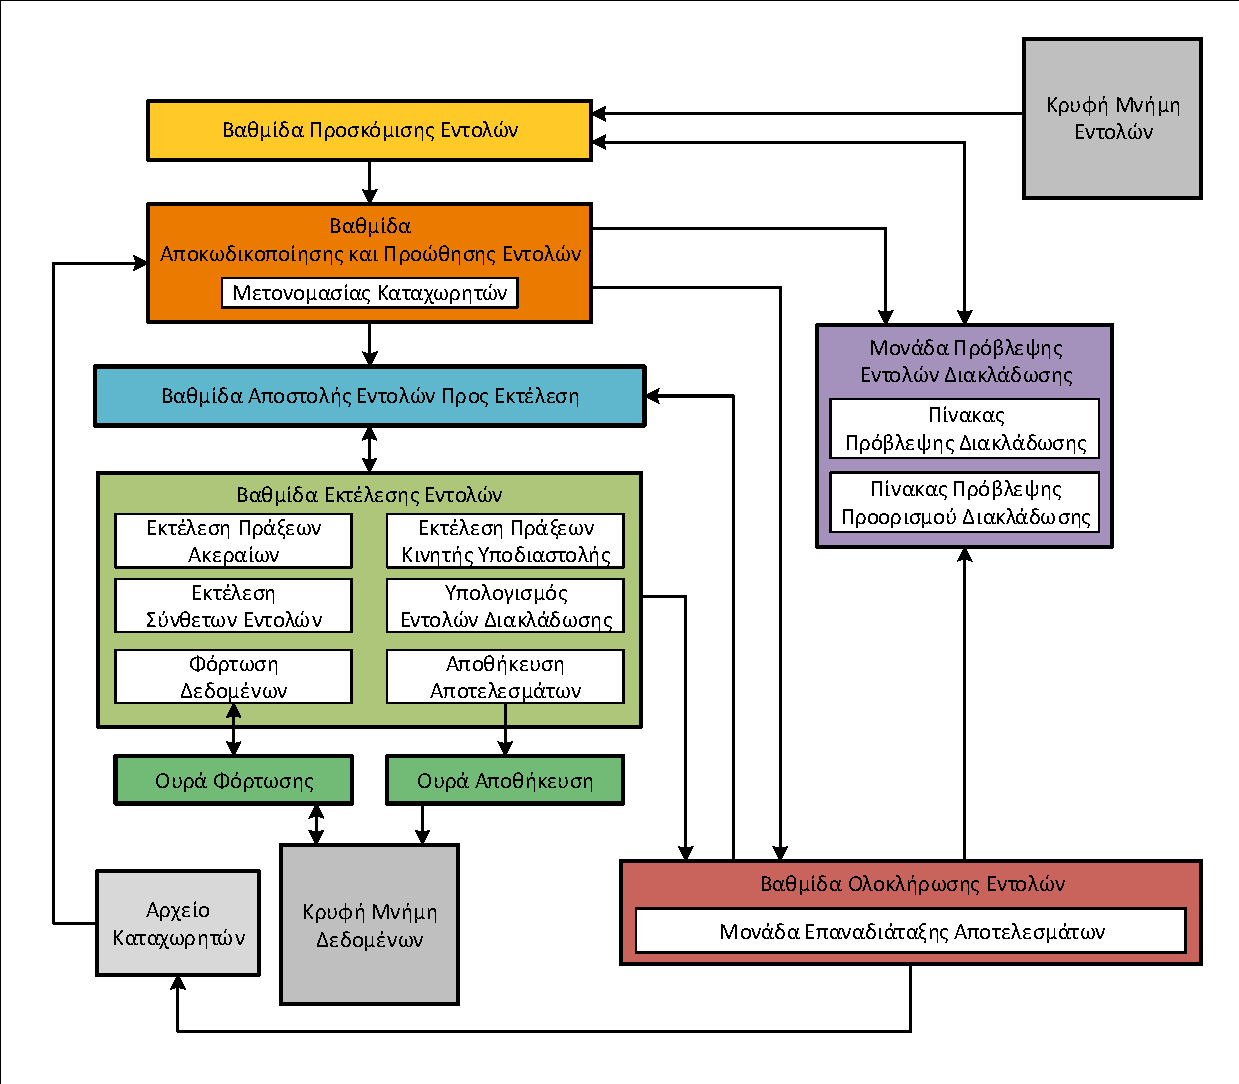
\includegraphics[width=0.95\linewidth, trim=0.5cm 0.8cm 0.5cm 0.5cm, clip=true]{\hardwareDIR/chap2_pipeline_stages.pdf}}
    \caption{Δομή Μηχανισμού Μερικώς Επικαλυπτόμενων Λειτουργιών}
    \label{fig:chap2_pipeline_stages}
\end{figure}

\section{Δομή και Οργάνωση του Δυναμικού Υπερβαθμωτού Επεξεργαστή}
\label{chap2_Superscalar}

Παρότι η δομή των υπερβαθμωτών επεξεργαστών εμφανίζει πλέον πολλές διαφοροποιήσεις μεταξύ σχεδιαστών και γενεών, οι μονάδες που τους αποτελούν μπορούν να διαχωριστούν σε πέντε βαθμίδες, όπως παρουσιάζονται στο Σχήμα \ref{fig:chap2_pipeline_stages}.

\subsubsection*{Προσκόμιση Εντολών}
\label{chap2_InstructionFetchUnit}

Στην πρώτη βαθμίδα ενός υπερβαθμωτού επεξεργαστή υλοποιείται ο μηχανισμός προσκόμιση εντολών από την Κρυφή Μνήμη Εντολών πρώτου επιπέδου. Σε κάθε κύκλο μπορούν να προσκομιστούν ένα σύνολο εντολών, το μέγιστο πλήθος των οποίων καθορίζεται από το πλάτος του υπερβαθμωτού επεξεργαστή.
\par
Για την απρόσκοπτη λειτουργία του μηχανισμού σε κάθε κύκλο πρέπει να είναι διαθέσιμες τόσες εντολές όσες και ο μέγιστος αριθμός εντολών που μπορούν να αποκωδικοποιηθούν ταυτόχρονα, διαδικασία η οποία εκτελείται στην αμέσως επόμενη βαθμίδα. Για το λόγο αυτό εισάγεται μια προσωρινή μνήμη εντολών στο τέλος της βαθμίδας προσκόμισης εντολών, στην οποία αποθηκεύονται οι εντολές που έχουν προσκομιστεί έως ότου προωθηθούν στη βαθμίδα αποκωδικοποίησης.
\par
Τέλος, προτού γίνει η προσκόμιση νέων εντολών στη βαθμίδα, προηγείται ο υπολογισμός της διεύθυνσης Κρυφής Μνήμης Εντολών στην οποία είναι αποθηκευμένες. Για το σκοπό αυτό, στη βαθμίδα προσκόμισης εντολών εμπεριέχονται και δυο ακόμα βασικά στοιχεία, η Μονάδα Υπολογισμού Διεύθυνσης της αμέσως επόμενης εντολής και η Μονάδα Δυναμικής Πρόβλεψης Διακλαδώσεων. Η Μονάδα Δυναμικής Πρόβλεψης Διακλαδώσεων αποτελεί τον κορμό της παρούσας διπλωματικής, επομένως η αναλυτική περιγραφή της λειτουργίας της πραγματοποιείται ξεχωριστά στην Ενότητα \ref{chap2_DynamicBranchPredictionUnit}.

\subsubsection*{Αποκωδικοποίηση και Προώθηση Εντολών}
\label{chap2_InstructionDecodeDispatch}

Βασική λειτουργία της δεύτερης βαθμίδα του υπερβαθμωτού επεξεργαστή είναι η αποκωδικοποίηση των εντολών χαμηλού επιπέδου σε μικροεντολές. Στη συνέχεια πραγματοποιείται ο έλεγχος εξαρτήσεων μεταξύ των εντολών καθώς και η προσκόμιση των τιμών των τελουμένων από το αρχείο καταχωρητών.
\par
Εξαιτίας της μεταβαλλόμενης σειράς εκτέλεσης των εντολών, μεταξύ των εντολών εμφανίζονται εξαρτήσεις δεδομένων οι οποίες καθιστούν αδύνατη την εκτέλεσή τους σε διαφορετική σειρά. Τα είδη των εξαρτήσεων δεδομένων εντάσσονται σε τρεις κατηγορίες:\\
\textit{Ανάγνωσης μετά από Εγγραφή (ΑμΕ) -} Όταν η Εντολή Β που μόλις αποκωδικοποιήθηκε αναμένει το αποτέλεσμα της προηγούμενης Εντολής Α, το οποίο χρησιμοποιείται ως τελούμενο από την Εντολή Β (καταχωρητής προορισμού Α = καταχωρητή πηγής Β).\\
\textit{Εγγραφή μετά από Εγγραφή (ΕμΕ) -} Όταν η Εντολή Β που μόλις αποκωδικοποιήθηκε αναμένει την εκτέλεση της προηγούμενης Εντολής Α, διότι και οι δύο αποθηκεύουν το αποτέλεσμά τους στον ίδιο καταχωρητή (καταχωρητής προορισμού Α = καταχωρητή προορισμού Β).\\
\textit{Εγγραφής μετά από Ανάγνωση (ΕμΑ) -} Όταν η Εντολή Β που μόλις αποκωδικοποιήθηκε αναμένει την εκτέλεση της προηγούμενης Εντολής Α, διότι η Εντολή Β αποθηκεύει τιμή στον ίδιο καταχωρητή από τον οποίο πραγματοποιεί ανάγνωση η εντολή Α (καταχωρητής πηγής Α = καταχωρητή προορισμού Β).
\par
Και οι τρεις αυτές περιπτώσεις εξαρτήσεων επιβάλουν την αδυναμία εκτέλεσης ορισμένων εντολών (Εντολή Β) έως ότου οι εξαρτήσεις παύσουν να ισχύουν, συνεπώς έως ότου εκτελεστούν οι προηγούμενες εντολές που αλληλεπιδρούν σε κοινούς καταχωρητές (Εντολή Α). Η συνεχής εμφάνιση εξαρτήσεων μπορεί να οδηγήσει σε σημαντική υποβάθμιση της απόδοσης του συστήματος. Από τα τρία είδη εξαρτήσεων που παρουσιάστηκαν, οι εξαρτήσεις τύπου ΕμΕ και ΕμΑ θα ήταν δυνατό να αποφευχθούν μέσω της χρήσης μεγαλύτερου πλήθους καταχωρητών από τις μικροεντολές. Οι εξαρτήσεις τέτοιου είδους αποκαλούνται αντεξαρτήσεις. Στους σύγχρονους υπερβαθμωτούς επεξεργαστές εισάγεται μία επιπλέον λειτουργία στη βαθμίδα αυτή η οποία αναλαμβάνει την επίλυση των αντεξαρτήσεων μέσω της αντιστοίχησης των αρχιτεκτονικών καταχωρητών, που χρησιμοποιούνται από τις εντολές χαμηλού επιπέδου, σε ένα μεγαλύτερο σύνολο φυσικών καταχωρητών που βρίσκονται εντός του Μηχανισμού Μερικώς Επικαλυπτόμενων Λειτουργιών. Η διαδικασία αυ΄τη αποκαλείται Μετονομασία Καταχωρητών και σε πολλές περιπτώσεις επεξεργαστών αποτελεί ξεχωριστή βαθμίδα.
\par
Μόλις ολοκληρωθεί και η μετονομασία των καταχωρητών μίας εντολής, αυτή προωθείται στην επόμενη βαθμίδα όπου αναμένει έως ότου όλα τα τελούμενα της είναι διαθέσιμα. Επιπλέον, η εντολή καταλαμβάνει μία θέση στη Μονάδα Επαναδιάταξης Αποτελεσμάτων, όπου συγκεντρώνονται τα αποτελέσματα των εντολών ώστε η ολοκλήρωσή τους να γίνεται με τη σωστή σειρά.

\subsubsection*{Αποστολή Εντολών Προς Εκτέλεση}
\label{chap2_InstructionIssue}

Οι εντολές που έχουν αποκωδικοποιηθεί και μετονομαστεί αποθηκεύονται σε μία προσωρινή μνήμη έως ότου είναι διαθέσιμα όλα τα τελούμενα που χρησιμοποιούν. Στου σύγχρονους υπερβαθμωτούς επεξεργαστές κάθε λειτουργική μονάδα έχει τη δική της προσωρινή μνήμη ώστε να διαχωρίζονται οι εντολές που αποστέλλονται από την προηγούμενη βαθμίδα. Οι μνήμες αυτές αποκαλούνται συνήθως Σταθμοί Κράτησης καθώς αποθηκεύονται τα τελούμενα που απαιτούνται από την εντολή, έως την εκτέλεση της. Μόλις όλα τα τελούμενα είναι διαθέσιμα και η αντίστοιχη λειτουργική μονάδα ελευθερωθεί πραγματοποιείται η προώθηση των τελουμένων της εντολής ώστε να πραγματοποιηθεί η εκτέλεσή της. Με το πέρας της εκτέλεσης γίνεται και η ενημέρωση όλων των Σταθμών Κράτησης που αναμένουν το αποτέλεσμα της συγκεκριμένης εντολής (εξαρτήσεις δεδομένων τύπου ΑμΕ).

\subsubsection*{Εκτέλεση Εντολών}
\label{chap2_InstructionExcecution}

Οι σύγχρονοι υπερβαθμωτοί επεξεργαστές αποτελούνται από ένα πλήθος διαφορετικών λειτουργικών μονάδων ώστε η κάθε μία να είναι βελτιστοποιημένη σε ένα συγκεκριμένο είδος πράξεων, με ορισμένες από αυτές να διαθέτουν τη δυνατότητα εκτέλεσης πολλαπλών εντολών στον ίδιο κύκλο ρολογιού. Στις πρώιμες εκδοχές των υπερβαθμωτών επεξεργαστών η μονάδα εκτέλεσης χρησιμοποιούταν τόσο για την εκτέλεση αριθμητικών πράξεων όσο για τον υπολογισμό διευθύνσεων μνήμης, την εκτέλεση εντολών διακλάδωσης, τη φόρτωση δεδομένων από την κρυφή μνήμη και την αποθήκευση αποτελεσμάτων σε αυτή. Πλέον συνηθίζεται οι λειτουργίες αυτές να υλοποιούνται από ξεχωριστές μονάδες. Η Μονάδα Υπολογισμού Διεύθυνσης υπολογίζει τη νέα τιμή του μετρητή προγράμματος, η οποία στην περίπτωση εντολών διακλάδωσης συγκρίνεται με την προβλεπόμενη διεύθυνση προσκόμισης. Αντίστοιχα, η Μονάδα Φόρτωσης/Αποθήκευσης συνδέεται απευθείας με την Κρυφή Μνήμη Δεδομένων για άμεση διαχείριση των δεδομένων από και προς αυτή.
\par
Ώς βαθμός παραλληλίας ορίζεται ο μέγιστος αριθμός εντολών που μπορούν να προσκομιστούν, να αποκωδικοποιηθούν ή να ολοκληρωθούν σε κάθε κύκλο. Στις πρώτες βαθμίδες ο χρόνος που απαιτείται σε κάθε μία δεν είναι σταθερός μεταξύ των διαφορετικών εντολών. Αντίθετα, στο στάδιο της εκτέλεσης ο χρόνος είναι σταθερός καθώς τα δεδομένα είναι όλα διαθέσιμα και πλέον αρκεί η εκτέλεση της απαιτούμενης ενέργειας. Για να μην εισάγεται καθυστέρηση στο στάδιο αυτό λόγω έλλειψης πόρων (δομικές εξαρτήσεις) ο συνολικός αριθμός λειτουργικών μονάδων πρέπει να υπερβαίνει το βαθμό παραλληλίας.
\par
Με το πέρας της εκτέλεσης γίνεται και η ενημέρωση όλων των Σταθμών Κράτησης που αναμένουν το αποτέλεσμα της συγκεκριμένης εντολής. Εξαιτίας της εκτέλεσης των εντολών με διαφορετική σειρά από αυτή του αρχικού προγράμματος, τα αποτελέσματα που εξάγεται από τις λειτουργικές μονάδες δεν επιτρέπεται να αποθηκευτούν στον αντίστοιχο αρχιτεκτονικό καταχωρητή έως ότου εκτελεστούν όλες οι εντολές που προηγούνται. Για το λόγο αυτό τα αποτελέσματα προωθούνται στην αντίστοιχη θέση που καταλαμβάνει η εντολή στη Μονάδα Επαναδιάταξης Αποτελεσμάτων, η οποία εντάσσεται στην αμέσως επόμενη βαθμίδα.

\subsubsection*{Ολοκλήρωση Εντολών}
\label{chap2_InstructionCommit}

Όταν μια εντολή περάσει όλες τις προηγούμενες βαθμίδες και το αποτέλεσμά της είναι διαθέσιμο στην έξοδο της λειτουργικής μονάδας, δεν μπορεί να θεωρηθεί ότι ολοκληρώθηκε διότι η σειρά ολοκλήρωσης των εντολών πρέπει να είναι ίδια με αυτή του αρχικού προγράμματος. Κατά τη διαδικασία ολοκλήρωσης μιας εντολής γίνεται και η τελική ενημέρωση του Αρχείου Αρχιτεκτονικών Καταχωρητών και της Κρυφής Μνήμης, εφόσον έχουν ολοκληρωθεί όλες οι εντολές που προηγούνται. Όπως αναφέρθηκε, για την υλοποίηση του σταδίου ολοκλήρωσης χρησιμοποιείται η Μονάδα Επαναδιάταξης Αποτελεσμάτων, στην οποία κάθε εντολή που αποκωδικοποιείται καταλαμβάνει μία θέση. Μόλις μία εντολή περάσει το στάδιο της εκτέλεσης γίνεται και η ενημέρωση των αντίστοιχων πεδίων της Μονάδας Επαναδιάταξης Αποτελεσμάτων. Κατά τη διάρκεια αναμονής των εντολών για την ολοκλήρωσή τους ενδέχεται να ανιχνευθεί εκτέλεση λανθασμένου μονοπατιού εξαιτίας μίας λανθασμένης πρόβλεψης κατά την προσκόμιση εντολής διακλάδωσης. Σε αυτή την περίπτωση, αρκεί να απορριφθούν από τη Μονάδα Επαναδιάταξης Αποτελεσμάτων και τα υπόλοιπα στοιχεία προσωρινής μνήμης όλων των βαθμίδων όσες εντολές ακολουθούν το σημείο στο οποίο έγινε η λανθασμένη πρόβλεψη, ώστε στη συνέχεια να γίνει η προσκόμιση των σωστών εντολών.

%----------------------------------------------------------%

\section{Μονάδα Δυναμικής Πρόβλεψης Διακλαδώσεων}
\label{chap2_DynamicBranchPredictionUnit}

Ένας πολύ σημαντικός παράγοντας στην αύξηση του απαιτούμενου χρόνου ολοκλήρωσης ενός προγράμματος του οποίου οι εντολές εκτελούνται εκτός σειράς, είναι η ύπαρξη πολλαπλών εντολών διακλάδωσης. Για την αδιάλειπτη εκτέλεση εντολών από την κεντρική μονάδα επεξεργασίας, κατά την προσκόμιση μίας εντολής διακλάδωσης είναι απαραίτητο να γίνεται πρόβλεψη του αποτελέσματος της ώστε να προσκομίζονται άμεσα οι εντολές που επακολουθούν. Εξάγεται δηλαδή μία πρόβλεψη εάν θα ληφθεί η διακλάδωση (αλλαγή της ροής του προγράμματος) ή όχι (διατήρηση της ροής εκτέλεσης). Εξαιτίας της μεγάλης σημασίας που έχει η εξαγωγή σωστής πρόβλεψης για την απόδοση του συστήματος, στον τομέα αυτό έχουν προταθεί πληθώρα τεχνικών παρέχοντας έτσι τη δυνατότητα συνεχούς προσκόμισης εντολών ακόμη και στην περίπτωση σημείων διακλάδωσης.
\par
Όπως ισχύει στην πλειοψηφία των επικρατέστερων τεχνικών, η πρόβλεψη των εντολών διακλάδωσης βασίζεται στο ιστορικό εκτέλεσης των προγραμμάτων και συχνά αποκαλείται δυναμική πρόβλεψη καθώς μεταβάλλεται με την πάροδο του χρόνου ώστε να βελτιστοποιείται η ακρίβειά της. Για το λόγο αυτό χρησιμοποιείται ένα σύνολο στοιχείων μνήμης εντός της βαθμίδας προσκόμισης, όπου και πραγματοποιείται η πρόβλεψη. Σε περίπτωση που η πρόβλεψη διακλάδωσης αποδειχθεί λανθασμένη η καθυστέρηση που εισάγεται στην εκτέλεση του προγράμματος καλείται ποινή αστοχίας διακλάδωσης και ισούται με τους κύκλους ρολογιού που καταναλώθηκαν από τη στιγμή πραγματοποιήθηκε η πρόβλεψη έως ότου ανιχνευθεί το λάθος της (εκτέλεση λάθος μονοπατιού εντολών).
\par
Καθώς το πλήθος των εντολών που μπορούν να αποκωδικοποιηθούν ταυτόχρονα αυξάνεται, η καθυστέρηση εξαιτίας μιας αστοχίας στην πρόβλεψη αποκτά ιδιαίτερη βαρύτητα καθώς μπορεί να οδηγήσει στην προσκόμιση μεγάλου πλήθους εντολών. Η μεταβολή της σειράς εκτέλεσης των εντολών εντός του Μηχανισμού Μερικώς Επικαλυπτόμενων Λειτουργιών σε συνδυασμό με την εισροή περιττών εντολών μπορεί να προκαλέσει αύξηση στον απαιτούμενο χρόνο ολοκλήρωσης του προγράμματος \cite{sendag2002effect}, οδηγώντας έτσι και σε αύξηση της απαιτούμενης ενέργειας. Από το γεγονός αυτό γίνεται φανερό πως η ορθότητα των προβλέψεων αποτελεί βασικό παράγοντα κατά τη σχεδίαση ενός υπερβαθμωτού επεξεργαστή, τόσο για τη βελτίωση της απόδοσης όσο και της κατανάλωσης.
\par
Στο Σχήμα \ref{fig:chap2_performance_without_prediction} παρουσιάζεται η επιβάρυνση που έχει ο ρυθμός ολοκλήρωσης εντολών (πλήθος εντολών που ολοκληρώνονται σε κάθε κύκλο - \ipc) όταν δεν χρησιμοποιείται μονάδα πρόβλεψης εντολών διακλάδωσης, σε σχέση με την περίπτωση όπου η κεντρική μονάδα επεξεργασίας διαθέτει κατάλληλο μηχανισμό πρόβλεψης εντολών διακλάδωσης. Η μείωση του ρυθμού φτάνει κατά μέσο ορό το 60\% ενώ σε ορισμένες περιπτώσεις ξεπερνά ακόμη και το 80\%. Τα αποτελέσματα απόδοσης που παρουσιάζονται τόσο στο παρόν όσο και στα επόμενα κεφάλαια εξήχθησαν με τη χρήση ενός εξομοιούμενου \en{x86} επεξεργαστή και με την εκτέλεση αντιπροσωπευτικών τμημάτων των μετροπρογραμμάτων \spec \cite{bird2007performance}. Η αναλυτική περιγραφή του περιβάλλοντος υλοποίησης των εξομοιώσεων πραγματοποιείται στα Κεφάλαια \ref{chap6} και \ref{chap7}.

\begin{figure}[t]
    \centering
    \fbox{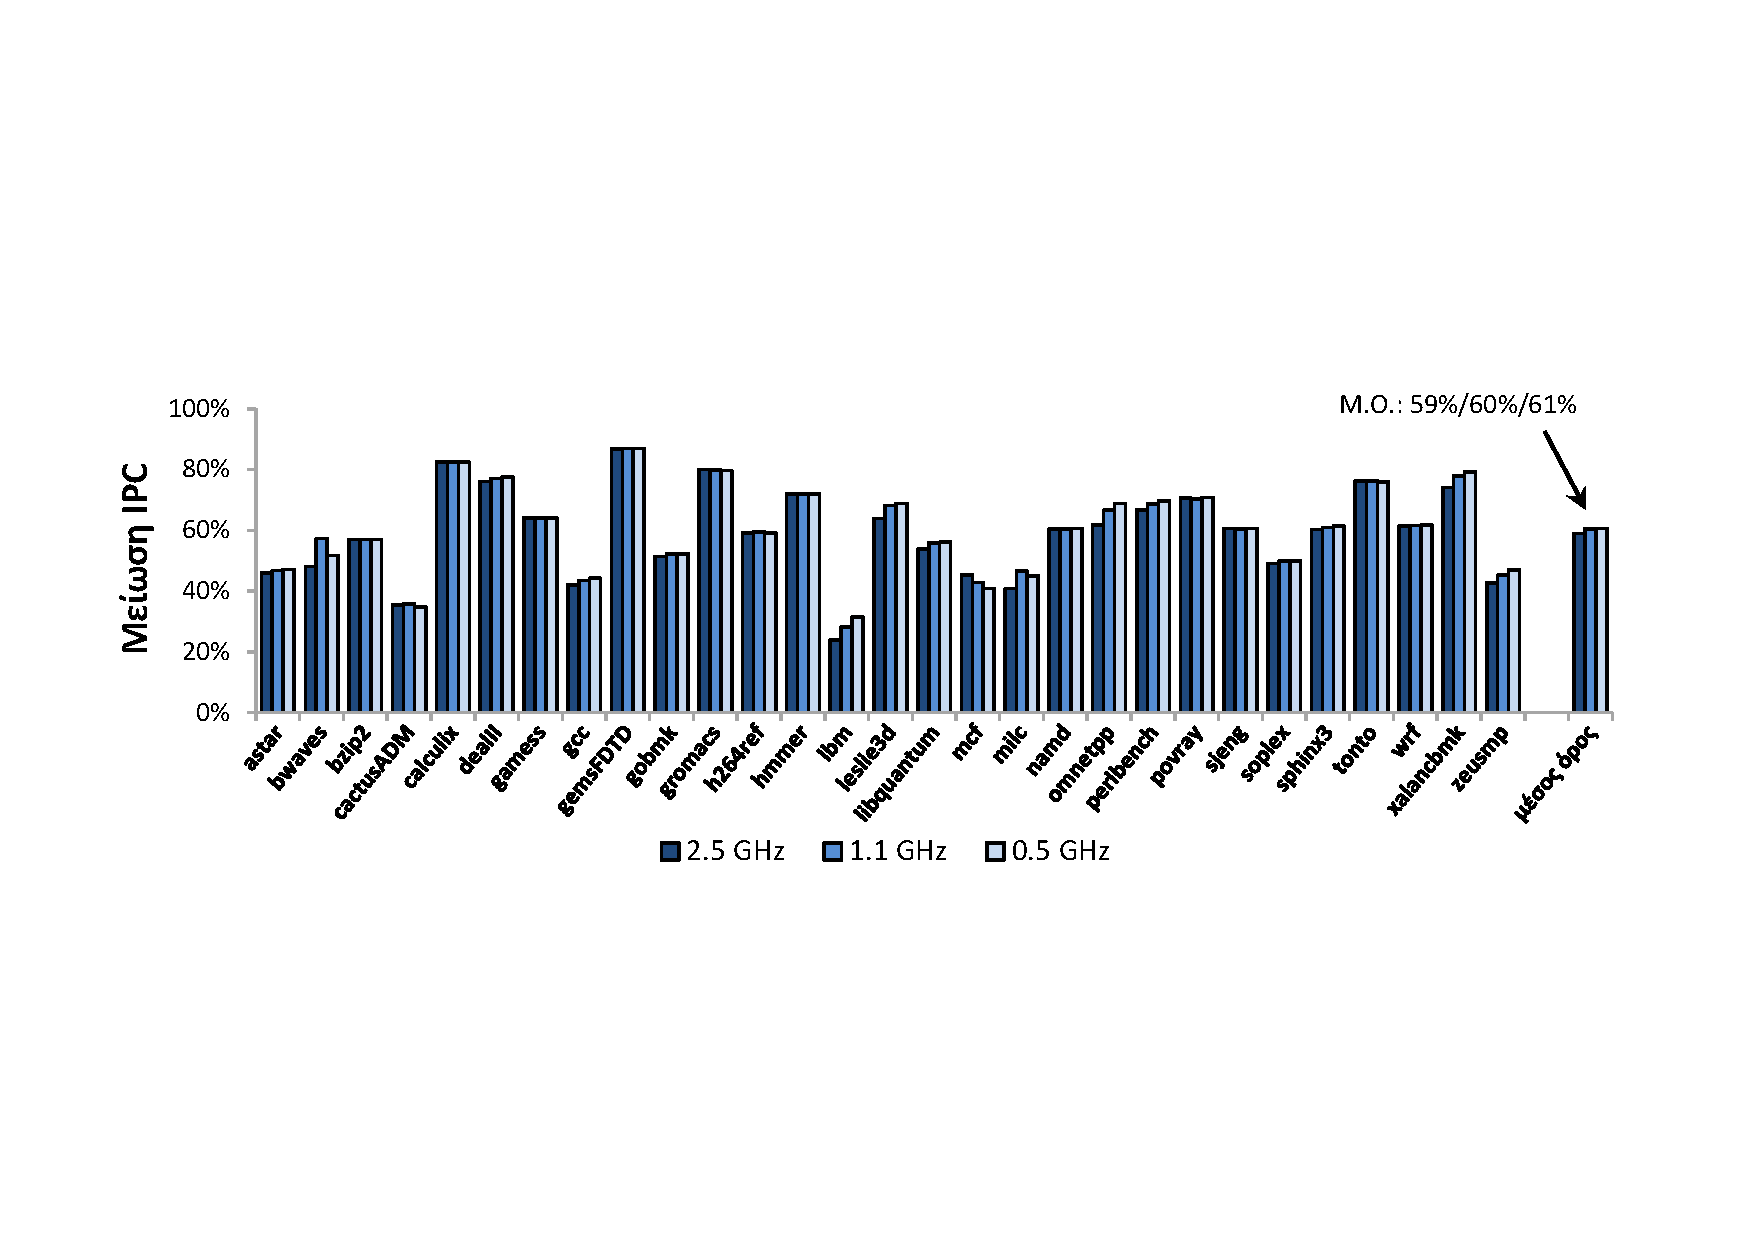
\includegraphics[width=\linewidth, trim=1.9cm 6.4cm 1.8cm 6.6cm, clip=true]{\resultsDIR/chap2_NoPrediction_NoBTB_ipc.pdf}}
    \caption{Ρυθμός ολοκλήρωσης εντολών όταν δεν διατίθεται μηχανισμός πρόβλεψης διακλαδώσεων, κανονικοποιημένος ως προς την περίπτωση που χρησιμοποιείται ο κατάλληλος μηχανισμός}
    \label{fig:chap2_performance_without_prediction}
\end{figure}

Στους σύγχρονους υπερβαθμωτούς επεξεργαστές, η Μονάδα Δυναμικής Πρόβλεψης Διακλαδώσεων \cite{smith1981study} αποτελείται από δύο βασικά στοιχεία. Το πρώτο και σημαντικότερο στοιχείο είναι ο Πίνακας Πρόβλεψης Διακλάδωσης \cite{pan1992improving, quinones2007improving}, η οποία περιέχει την κατάλληλη πληροφορία ώστε να γίνει η πρόβλεψη εάν η εκτέλεση πρέπει να συνεχιστεί στην αμέσως επόμενη εντολή (μη λήψη της διακλάδωσης) ή σε κάποιο άλλο σημείο του προγράμματος (λήψη της διακλάδωσης), δηλαδή εάν θα ικανοποιηθεί η συνθήκη της εντολής διακλάδωσης ή όχι. Το δεύτερο στοιχείο της Μονάδας Δυναμικής Πρόβλεψης Διακλαδώσεων αποτελεί ο Πίνακας Πρόβλεψης Προορισμού Διακλάδωσης \cite{bray1991strategies, perleberg1993branch}. Ο συγκεκριμένος πίνακας αποτελεί μία μνήμη η οποία παρέχει τη διεύθυνση εντολής στην οποία προβλέπεται να μετατοπιστεί η εκτέλεση, σε περίπτωση που έχει προβλεφθεί λήψη της διακλάδωσης από το πρώτο στοιχείο. Η χρήση ενός μηχανισμού πρόβλεψης διακλαδώσεων συνεπάγεται και την ανάγκη για υλοποίηση κατάλληλου μηχανισμού επαναφοράς σε περίπτωση λανθασμένης πρόβλεψης. Η γενική δομή της Μονάδας Δυναμικής Πρόβλεψης Διακλαδώσεων παρουσιάζεται στο Σχήμα \ref{fig:chap2_abstract_predictor}.

\begin{figure}[!b]
    \centering
    \fbox{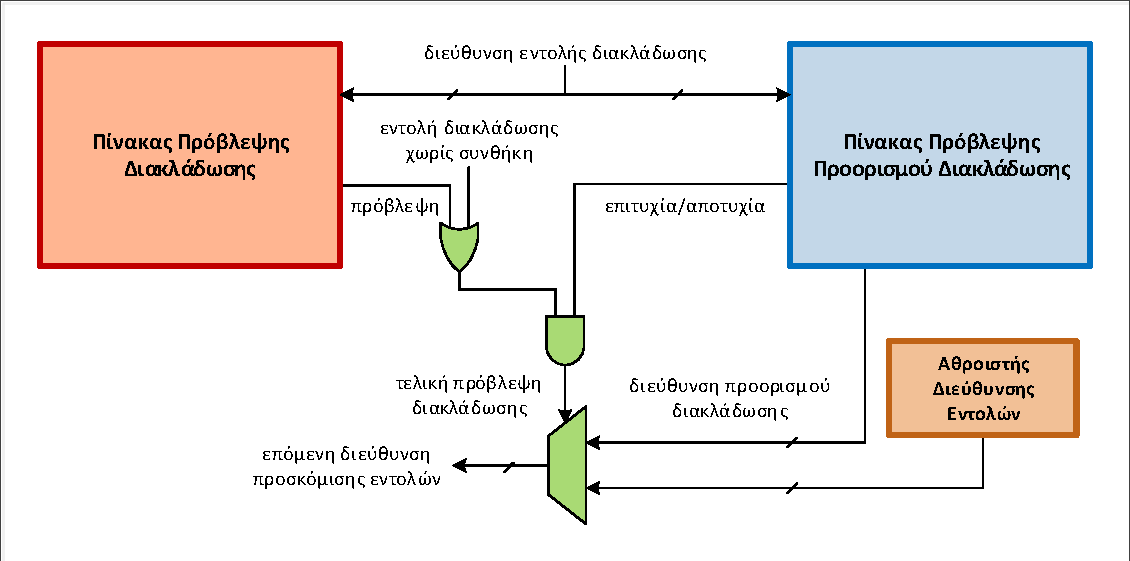
\includegraphics[width=\linewidth, trim=0.5cm 0.65cm 0.5cm 0.7cm, clip=true]{\hardwareDIR/chap2_abstract_predictor.pdf}}
    \caption{Περιληπτική δομή της Μονάδας Δυναμικής Πρόβλεψης Διακλαδώσεων}
    \label{fig:chap2_abstract_predictor}
\end{figure}

%----------------------------------------------------------%

\subsection{Πίνακας Πρόβλεψης Διακλάδωσης}
\label{chap2_BranchPredictor}

Πληθώρα τεχνικών έχουν προταθεί για την υλοποίηση του Πίνακα Πρόβλεψης Διακλάδωσης. Οι τεχνικές αυτές μπορούν να ομαδοποιηθούν σε τρεις κατηγορίες αναλόγως του τρόπου εξαγωγής πρόβλεψης: αυτές που έχουν ως δεδομένο την τρέχουσα τιμή του μετρητή προγράμματος, αυτές που διατηρούν ιστορικό εκτέλεσης των εντολών διακλάδωσης, και τέλος τις συνδυαστικές.
\par
Οι τεχνικές που χρησιμοποιούνται ευρέως στους σύγχρονους επεξεργαστές ανήκουν στην κατηγορία των συνδυαστικών προβλεπτών \cite{cummins2001branch}. Για το λόγο αυτό χρησιμοποιούν ένα ή περισσότερα στοιχεία μνήμης όπου γίνεται η αποθήκευση του ιστορικού διακλαδώσεων ώστε μελλοντικά να μπορεί να πραγματοποιείται μεγαλύτερης ακριβείας πρόβλεψη, με βάση αυτό το ιστορικό. Η τελική πληροφορία που παρέχεται αποτελείται από ένα δυαδικό ψηφίο το οποίο δηλώνει εάν προβλέπεται ότι η μετατόπιση της ροής θα γίνει ή όχι (λήψη/μη λήψη διακλάδωσης). Τον πυρήνα της πρόβλεψης αποτελεί ο αποκαλούμενος Πίνακας Πρόβλεψης Διακλάδωσης ή Πίνακας Ιστορικού Διακλάδωσης, ο οποίος συνήθως αποτελείται από ένα σύνολο μετρητών των δύο δυαδικών ψηφίων. Με τον υπολογισμό του αποτελέσματος της εντολής διακλάδωσης ο αντίστοιχος μετρητής ενημερώνεται κατάλληλα ώστε να γίνει η μετάβαση κατάστασης, όπως φαίνεται και στο διάγραμμα καταστάσεων τους Σχήματος \ref{fig:chap2_2bit_prediction_fsm}.

\begin{figure}[t]
    \centering
    \fbox{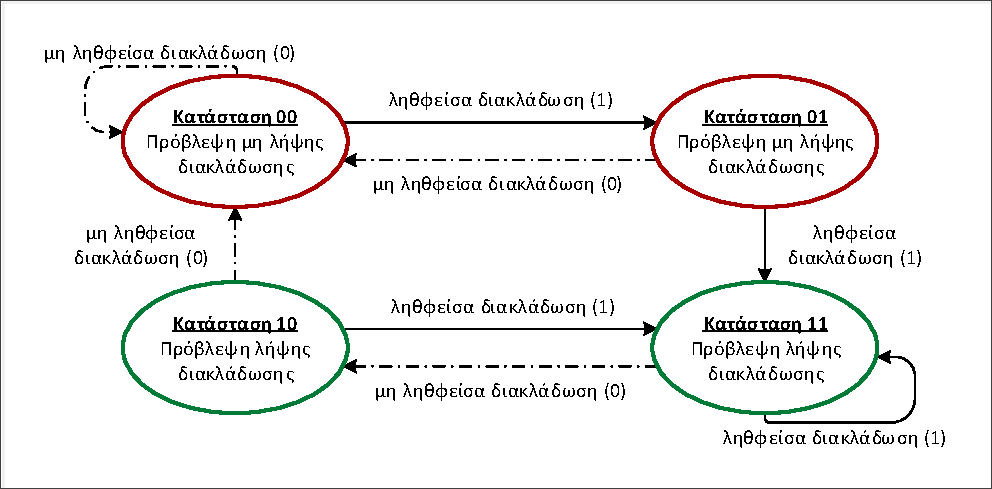
\includegraphics[width=\linewidth, trim=0.3cm 0.7cm 0.3cm 0.7cm, clip=true]{\hardwareDIR/chap2_2bit_prediction_fsm.pdf}}
    \caption{Δυναμική πρόβλεψη δύο δυαδικών ψηφίων}
    \label{fig:chap2_2bit_prediction_fsm}
\end{figure}

Στους μετρητές ιστορικού οι τιμές ‘00’ και ‘01’ αντιστοιχούν σε διατήρηση της ροής εκτέλεσης εντολών (πρόβλεψη μη λήψης διακλάδωσης), σε αντίθεση με τις τιμές ‘10’ και ‘11’ όπου συνεπάγεται πρόβλεψη μετατόπισης της εκτέλεσης (πρόβλεψη λήψης διακλάδωσης). Η ενημέρωση της κατάστασης υλοποιείται μέσω της ολίσθησης των περιεχομένων του αντίστοιχου μετρητή. Επομένως, θεωρώντας πως αρχικά οι μετρητές έχουν τιμή ‘00’, εάν η πρώτη εντολή διακλάδωσης αποδειχθεί πως είναι ληφθείσα (αλλαγή τη ροής) η τιμής του αντίστοιχου μετρητή θα ολισθήσει κατά μία θέση αριστερά και στο λιγότερο σημαντικό ψηφίο θα εισαχθεί το 1 με αποτέλεσμα ο μετρητής να έχει πλέον την τιμή ‘01’. Εάν στην επόμενη εκτέλεση της ίδιας εντολής διακλάδωσης παρουσιαστεί η ίδια συμπεριφορά η τιμή του μετρητή θα γίνει ‘11’. Τη στιγμή που η εντολή αλλάξει τη συμπεριφορά της και η εντολή διακλάδωσης γίνει μη ληφθείσα (η ροή εκτέλεσης παραμένει σταθερή), η τιμή του μετρητή θα ολισθήσει κατά μία θέση αριστερά όπως προηγουμένως, όμως στο λιγότερο σημαντικό ψηφίο θα εισαχθεί το 0. Ώς αποτέλεσμα, η τιμή του μετρητή θα γίνει ‘10’. Αντιστοίχως, την επόμενη φορά που η εντολή διακλάδωσης θα αποδειχθεί μη ληφθείσα ο μετρητής θα πάρει τη τιμή ‘00’.
\par
Στην πραγματικότητα η πρόβλεψη δεν αναφέρεται αποκλειστικά στη συγκεκριμένη εντολή διακλάδωσης αλλά σε ένα πλήθος αυτών, διότι διαφορετικά θα απαιτούνταν στοιχεία μνήμης πολύ μεγάλου μεγέθους για την εξυπηρέτηση όλων των εντολών διακλάδωσης. Η διευθυνσιοδότηση των χρησιμοποιούμενων στοιχείων μνήμης γίνεται είτε από το χαμηλότερο τμήμα της διεύθυνσης των εντολών διακλάδωσης είτε από κάποιο ειδικό καταχωρητή. Το γεγονός αυτό δεν επηρεάζει το αποτέλεσμα της εκτέλεσης. Η μόνη επίπτωση που μπορεί να έχει είναι η μείωση της απόδοσης σε περίπτωση που το ιστορικό έχει αλλοιωθεί εξαιτίας της προσκόμισης και άλλων εντολών διακλάδωσης που επιδρούν στην ίδια θέση μνήμης. Η εξαγωγή μιας λανθασμένης πρόβλεψης θα οδηγήσει στην εκτέλεση λανθασμένου συνόλου εντολών, οι οποίες όμως δεν θα ολοκληρωθούν. Συνεπώς δεν θα αλλοιωθούν τα δεδομένα της κρυφής μνήμης και των καταχωρητών, διότι τα αποτελέσματά των εντολών αναμένουν στη Μονάδα Επαναδιάταξης Αποτελεσμάτων, όπως αναφέρθηκε στην Ενότητα \ref{chap2_Superscalar}. Όταν η εντολή διακλάδωσης εκτελεστεί και αποκαλυφθεί πως έχει ακολουθηθεί λάθος μονοπάτι εντολών, θα εκτελεστεί η διαδικασία απόρριψης εντολών από το Μηχανισμό Μερικώς Επικαλυπτόμενων Λειτουργιών καθώς και η απαραίτητη ενημέρωση της μονάδας πρόβλεψης. Στη συνέχεια γίνεται η προσκόμιση των σωστών εντολών από την Κρυφή Μνήμη Εντολών.

\begin{figure}[!b]
    \centering
    \fbox{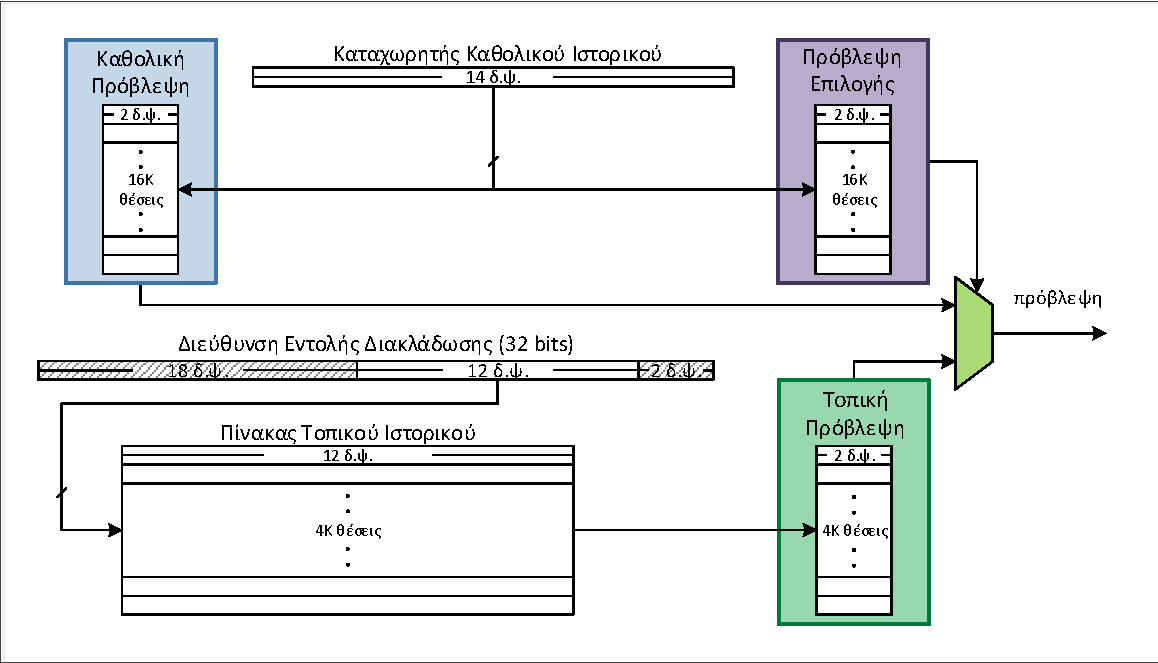
\includegraphics[width=\linewidth, trim=0.45cm 0.6cm 0.45cm 0.6cm, clip=true]{\hardwareDIR/chap2_tournament_predictor.pdf}}
    \caption{Δομή Πρόβλεψης Επιλεκτικής Διάταξης}
    \label{fig:chap2_tournament_predictor}
\end{figure}

Μια από τις πιο διαδεδομένες τεχνικές πρόβλεψης των σύγχρονων υπερβαθμωτών επεξεργαστών είναι η Πρόβλεψη Επιλεκτικής Διάταξης \cite{kessler1998alpha}, η οποία χρησιμοποιεί ένα πλήθος στοιχείων μνήμης ώστε σε κάθε περίπτωση διακλάδωσης να χρησιμοποιηθεί αυτή που έχει μεγαλύτερη πιθανότητα ευστοχίας. Η δομή της τεχνικής αυτής παρουσιάζεται αναλυτικά στο Σχήμα \ref{fig:chap2_tournament_predictor}.
\par
Στην πρόβλεψη επιλεκτικής διάταξης χρησιμοποιούνται δύο διατάξεις εξαγωγής πρόβλεψης διακλάδωσης καθώς και μία διάταξη για την επιλογή της κατάλληλης πρόβλεψης διακλάδωσης. Κάθε στοιχείο πρόβλεψης αποτελείται από ένα πίνακα μετρητών, με κάθε μετρητή να αντιστοιχεί σε ένα σύνολο εντολών. Στην περίπτωση των προβλέψεων διακλάδωσης (Καθολική και Τοπική Πρόβλεψη), το πιο σημαντικό ψηφίο κάθε θέσης του πίνακα μετρητών δηλώνει εάν προβλέπεται να γίνει λήψη ή όχι της διακλάδωσης. Η διάταξη επιλογής (Πρόβλεψη Επιλογής) αποτελείται επίσης από ένα πίνακα μετρητών οπού το πιο σημαντικό ψηφίο κάθε θέσης δηλώνει εάν θα χρησιμοποιηθεί η Καθολική ή η Τοπική Πρόβλεψη. Για τη δεικτοδότηση των μετρητών χρησιμοποιούνται κάποια στοιχεία αποθήκευσης ιστορικού, όπως παρουσιάζεται και στο Σχήμα \ref{fig:chap2_tournament_predictor}.

\subsubsection*{Καταχωρητής Καθολικού Ιστορικού}
\label{chap2_GlobalHistoryBuffer}

Το περιεχόμενό του χρησιμοποιείται για τη διευθυνσιοδότηση τόσο του πίνακα μετρητών της Καθολικής Πρόβλεψης όσο και του αντίστοιχου πίνακα της Πρόβλεψης Επιλογής, επομένως το μέγεθός του εξαρτάται από το πλήθος των μετρητών τους. Κάθε φορά που εξάγεται μία πρόβλεψη από τον Πίνακα Πρόβλεψης Διακλάδωσης, πραγματοποιείται και η ενημέρωση του καταχωρητή. Τα περιεχόμενά του ολισθαίνουν κατά μία θέση προς τα αριστερά και εάν η πρόβλεψη που εξάγεται δηλώνει λήψη της διακλάδωσης το τελευταίο δυαδικό ψηφίο παίρνει την τιμή 1, διαφορετικά την τιμή 0. Σε περίπτωση που η πρόβλεψη αποδειχθεί λανθασμένη, κατά τη διαδικασία απόρριψης των περιττών εντολών γίνεται και η ενημέρωση των περιεχομένων του. Τα περιεχόμενά ολισθαίνουν κατά μία θέση προς τα αριστερά και εάν έγινε λήψη της διακλάδωσης το τελευταίο δυαδικό ψηφίο παίρνει την τιμή 1, διαφορετικά την τιμή 0.

\subsubsection*{Καθολική Πρόβλεψη}
\label{chap2_GlobalPrediction}

Παρέχει μία πρόβλεψη με βάση τη συνολική συμπεριφορά του προγράμματος και όχι της συγκεκριμένης εντολής διακλάδωσης που προσκομίζεται. Αποτελείται από ένα πίνακα μετρητών, συνήθως των δύο δυαδικών ψηφίων. Σε κάθε προσκόμιση εντολής διακλάδωσης το περιεχόμενο του Καταχωρητή Καθολικού Ιστορικού ορίζει ποιο στοιχείο του πίνακα θα παρέχει την πρόβλεψη, η οποία οδηγείται έως τον πολυπλέκτη που ελέγχει η Πρόβλεψη Επιλογής. Όταν υπολογιστεί το αποτέλεσμα της εντολής διακλάδωσης γίνεται η κατάλληλη ενημέρωση του μετρητή που δείχνει ο Καταχωρητής Καθολικού Ιστορικού. Εάν το αποτέλεσμα της εντολής είναι λήψη της διακλάδωσης η τιμή του συγκεκριμένου μετρητή αυξάνεται κατά 1, στην αντίθετη περίπτωση η τιμή του μειώνεται κατά 1. Ο μετρητής που θα ενημερωθεί μπορεί να διαφέρει από αυτόν που χρησιμοποιήθηκε κατά την πρόβλεψη της συγκεκριμένης εντολής διότι μεταξύ της προσκόμισης και της εκτέλεσης της ενδέχεται να έχουν προσκομιστεί και άλλες εντολές διακλάδωσης μεταβάλλοντας έτσι το περιεχόμενο του Καταχωρητή Καθολικού Ιστορικού.

\subsubsection*{Πίνακας Τοπικού Ιστορικού}
\label{chap2_LocalHistoryTable}

Αποτελείται από ένα σύνολο στοιχείων μνήμης πολλαπλών δυαδικών ψηφίων όπου κάθε θέση αντιστοιχεί σε ένα σύνολο εντολών διακλάδωσης, σε αντίθεση με τον Καταχωρητή Καθολικού Ιστορικού ο οποίος αντιστοιχεί σε όλες τις εντολές διακλάδωσης. Η δανειοδοτούμενη θέσης χρησιμοποιείται για τη διευθυνσιοδότηση του πίνακα μετρητών της Τοπικής Πρόβλεψης και ενημερώνεται κατάλληλα όταν εξάγεται μία πρόβλεψη από τον Πίνακα Πρόβλεψης Διακλάδωσης. Σε αντιστοιχία με τον Καταχωρητή Καθολικού Ιστορικού, κάθε φορά που γίνεται μία πρόβλεψη το περιεχόμενο της δεικτοδοτούμενης θέσης του πίνακα ολισθαίνει κατά μία θέση προς τα αριστερά. Όταν προβλέπεται πως θα γίνει λήψη της διακλάδωσης το τελευταίο δυαδικό ψηφίο παίρνει την τιμή 1, διαφορετικά την τιμή 0. Η διευθυνσιοδότηση του πίνακα γίνεται από τα χαμηλότερης τάξης δυαδικά ψηφία της διεύθυνσης της εντολής διακλάδωσης. Κατά τη διαδικασία απόρριψης εντολών σε περίπτωση αποτυχίας πρόβλεψης γίνεται και η ενημέρωση των περιεχομένων της θέσης που δεικτοδοτείται. Η τιμή της ολισθαίνει κατά μία θέση προς τα αριστερά και εάν έγινε λήψη της διακλάδωσης το τελευταίο δυαδικό ψηφίο παίρνει την τιμή 1, διαφορετικά την τιμή 0.

\subsubsection*{Τοπική Πρόβλεψη}
\label{chap2_LocalPrediction}

Παρέχει μία πρόβλεψη με βάση τη συμπεριφορά ενός περιορισμένου συνόλου εντολών διακλάδωσης. Αποτελείται από ένα πίνακα μετρητών, συνήθως των δύο ή τριών δυαδικών ψηφίων για μεγαλύτερη ακρίβεια πρόβλεψης (8 καταστάσεις αντί για 4 στο διάγραμμα καταστάσεων του Σχήματος \ref{fig:chap2_2bit_prediction_fsm}). Όταν γίνεται προσκόμιση μίας εντολής διακλάδωσης μία από τις θέσεις του Πίνακα Τοπικού Ιστορικού καθορίζει ποια θέση του πίνακα θα παρέχει την πρόβλεψη, η οποία οδηγείται στην δεύτερη είσοδο του πολυπλέκτη που ελέγχει η Πρόβλεψη Επιλογής. Όταν υπολογιστεί το αποτέλεσμα της εντολής διακλάδωσης γίνεται και η κατάλληλη ενημέρωση του δεικτοδοτούμενου μετρητή. Εάν το αποτέλεσμα της εντολής είναι λήψη της διακλάδωσης η τιμή του συγκεκριμένου μετρητή αυξάνεται κατά 1, στην αντίθετη περίπτωση η τιμή του μειώνεται κατά 1. Ομοίως με την περίπτωση της Καθολικής Πρόβλεψης, ο μετρητής που θα ενημερωθεί μπορεί να διαφέρει από αυτόν που χρησιμοποιήθηκε κατά την πρόβλεψη της συγκεκριμένης εντολής, εξαιτίας της μεταβολής των περιεχομένων του Πίνακα Τοπικού Ιστορικού.

\subsubsection*{Πρόβλεψη Επιλογής}
\label{chap2_ChoicePrediction}

Παρέχει την πρόβλεψη για τη σωστή επιλογή μεταξύ της Τοπικής και της Καθολικής Πρόβλεψης, με βάση τη συνολική συμπεριφορά του προγράμματος. Αποτελείται από ένα πίνακα μετρητών, συνήθως των δύο δυαδικών ψηφίων και μεγέθους όσο και ο αντίστοιχος πίνακας της Καθολικής Πρόβλεψης. Το περιεχόμενο του Καταχωρητή Καθολικού Ιστορικού ορίζει ποια θέση του πίνακα θα παρέχει την πρόβλεψη επιλογής, και το πιο σημαντικό ψηφίο αυτής της θέσης οδηγείται στην είσοδο ελέγχου του πολυπλέκτη. Όταν υπολογιστεί το αποτέλεσμα της εντολής διακλάδωσης γίνεται η κατάλληλη ενημέρωση του μετρητή που δείχνει ο Καταχωρητής Καθολικού Ιστορικού, εάν και μόνο εάν οι προβλέψεις των δύο διατάξεων (Καθολική/Τοπική) διαφέρουν μεταξύ τους. Εάν το αποτέλεσμα της διακλάδωσης συμπίπτει με την Τοπική Πρόβλεψη η τιμή του συγκεκριμένου μετρητή μειώνεται κατά 1, διαφορετικά αυξάνεται κατά 1. Όπως με την περίπτωση της Καθολικής Πρόβλεψης, ο μετρητής που θα ενημερωθεί μπορεί να διαφέρει από αυτόν που χρησιμοποιήθηκε κατά την πρόβλεψη της εντολής.

\subsubsection*{Διάγραμμα Ενημέρωσης Στοιχείων Πρόβλεψης}
\label{chap2_PredictionUpdate}

Στο Σχήμα \ref{fig:chap2_predictor_update} παρουσιάζονται διαγραμματικά οι συνθήκες που ισχύουν για την ενημέρωση των στοιχείων μνήμης που αποτελούν τον Πίνακα Πρόβλεψης Διακλάδωσης. Oι συμβολισμοί $``\ +$1 $"$, $``\ -$1 $"$, $``\ <<1\ "$ και $``\ <<1$ \& +1 $"$ ισοδυναμούν με αύξηση κατά μία μονάδα, μείωση κατά μία μονάδα, αριστερή ολίσθηση κατά ένα δυαδικό ψηφίο, αριστερή ολίσθηση κατά ένα δυαδικό ψηφίο και εισαγωγή της μονάδας στο λιγότερο σημαντικό ψηφίο αντίστοιχα.

\begin{figure}[!h]
    \centering
    \fbox{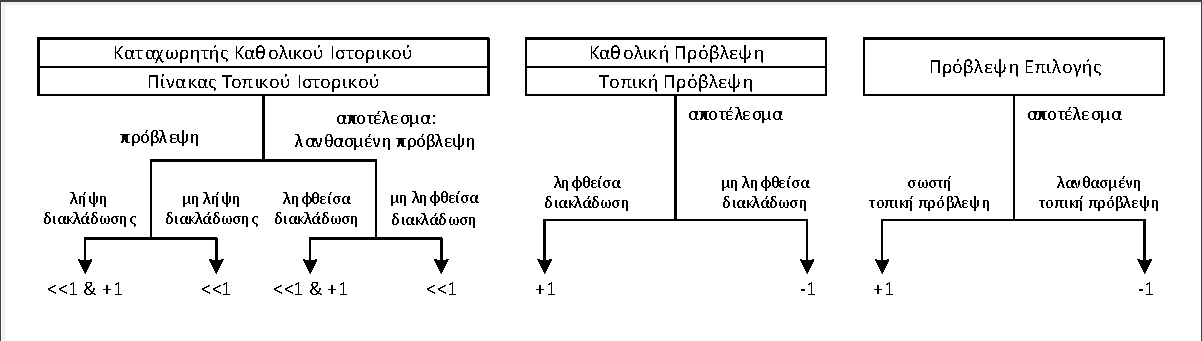
\includegraphics[width=\linewidth, trim=0.5cm 0.8cm 0.5cm 0.6cm, clip=true]{\hardwareDIR/chap2_predictors_update.pdf}}
    \caption{Μεθοδολογία ενημέρωσης των στοιχείων που συμβάλουν στην πρόβλεψη}
    \label{fig:chap2_predictor_update}
\end{figure}

%----------------------------------------------------------%

\subsection{Πίνακας Πρόβλεψης Προορισμού Διακλάδωσης}
\label{chap2_BranchTargetBuffer}

Σε μία σύγχρονη αρχιτεκτονική περικλείονται πολλών ειδών εντολές διακλάδωσης, οι οποίες παρουσιάζουν σημαντικές διαφορές στη συμπεριφορά τους και για το λόγο αυτό κατηγοριοποιούνται. Συνεπώς, προτού γίνει εμβάθυνση στη λειτουργία της συγκεκριμένης μνήμης είναι απαραίτητο να αποσαφηνιστούν οι διαφορές μεταξύ τους. Στην ακόλουθη περιγραφή των κατηγοριών, για κάθε κατηγορίας εντολής διακλάδωσης δίνεται και ένα παράδειγμα από το σύνολο εντολών αρχιτεκτονικής \en{MIPS} \cite{price1995mips}.
\par
Οι εντολές διακλάδωσης που προσκομίζονται στο Μηχανισμό Μερικώς Επικαλυπτόμενων Λειτουργιών διαχωρίζονται στις ακόλουθες δύο κατηγορίες:\\
\indent\textbf{\textit{Άμεσης Διευθυνσιοδότησης -}} Η διεύθυνση στην οποία θα μεταβεί η εκτέλεση σε περίπτωση που γίνει λήψη της διακλάδωσης αποτελεί τμήμα της εντολής και είναι ήδη γνωστή. Παράδειγμα τέτοιου είδους εντολής διακλάδωσης αποτελεί η εντολή \en{J} ενός επεξεργαστή \en{MIPS}.\\
\indent\textbf{\textit{Έμμεσης Διευθυνσιοδότησης -}} Η διεύθυνση στην οποία θα μεταβεί η εκτέλεση σε περίπτωση που γίνει λήψη της διακλάδωσης δεν είναι γνωστή εκ των προτέρων, ως εκ τούτου απαιτείται επιπλέον χρόνο για τον υπολογισμό της. Ο Πίνακας Πρόβλεψης Προορισμού Διακλάδωσης διατηρεί ένα ιστορικό των διευθύνσεων διακλάδωσης με βάση την προηγούμενη συμπεριφορά των εντολών, ώστε να παρέχει μία πρόβλεψης της διεύθυνσης στην οποία θα μεταφερθεί η εκτέλεση του προγράμματος προτού γίνει ο πραγματικός υπολογισμός της για την επαλήθευση της πρόβλεψης. Παράδειγμα τέτοιου είδους εντολής διακλάδωσης στον \en{MIPS} αποτελεί η εντολή \en{JR}.
\par
Επιπλέον, οι εντολές διακλάδωσης (άμεσης και έμμεσης διευθυνσιοδότησης) μπορούν να διαχωριστούν στις ακόλουθες δύο υποκατηγορίες:\\
\indent\textbf{\textit{Χωρίς Συνθήκη -}} Η συμπεριφορά της εντολής διακλάδωσης είναι προκαθορισμένη και επομένως το μόνο που απαιτείται είναι μία πρόβλεψη της διεύθυνσης στην οποία θα γίνει η μετατόπιση της εκτέλεσης. Όταν η εντολή είναι έμμεσης διευθυνσιοδότηση η πληροφορία αυτή λαμβάνεται από τον Πίνακα Πρόβλεψης Προορισμού Διακλάδωσης, εάν είναι διαθέσιμη. Παράδειγμα τέτοιου είδους εντολής διακλάδωσης στον \en{MIPS} αποτελεί η εντολή \en{JR}.\\
\indent\textbf{\textit{Υπό Συνθήκη -}} Ο Πίνακας Πρόβλεψης Διακλάδωσης παρέχει την πρόβλεψη εάν θα γίνει λήψη της διακλάδωση καθώς δεν είναι γνωστή εκ των προτέρων η συμπεριφορά των εντολών αυτού του είδους. Σε περίπτωση που προβλέπεται λήψη της διακλάδωσης και η εντολή είναι έμμεσης διευθυνσιοδότηση, ο Πίνακας Πρόβλεψης Προορισμού Διακλάδωσης παρέχει μία πρόβλεψη της διεύθυνσης μετατόπισης της ροής εκτέλεσης, εάν έχει διαθέσιμη την πληροφορία αυτή. Παράδειγμα τέτοιου είδους εντολής διακλάδωσης στον \en{MIPS} αποτελεί η εντολή \en{BEQ}.
\par
Επομένως, στην περίπτωση των εντολών έμμεσης διευθυνσιοδότησης η γνώση - πρόβλεψη της διεύθυνσης στην οποία θα μεταφερθεί η εκτέλεση αποτελεί σημαντικό πλεονέκτημα για την επικάλυψη του χρόνου καθυστέρησης που εισάγεται έως τον υπολογισμό της.

\begin{figure}[!b]
    \centering
    \fbox{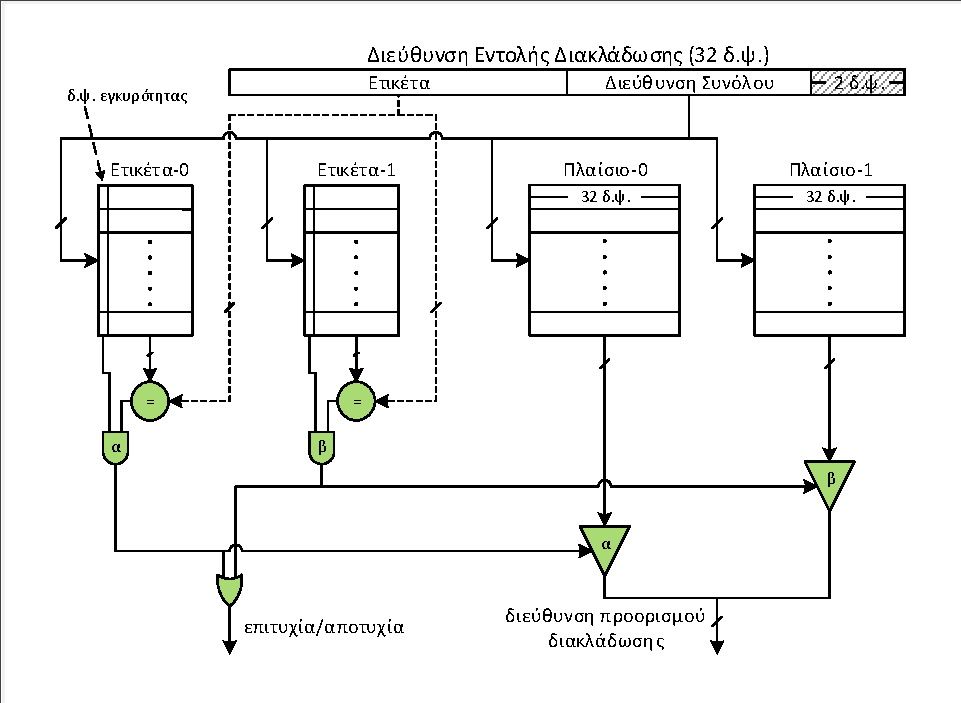
\includegraphics[width=\linewidth, trim=0.5cm 0.8cm 0.5cm 0.7cm, clip=true]{\hardwareDIR/chap2_btb.pdf}}
    \caption{Δομή Πίνακα Πρόβλεψης Προορισμού Διακλάδωσης}
    \label{fig:chap2_branch_target_buffer}
\end{figure}

\par
Ο Πίνακας Πρόβλεψης Προορισμού Διακλάδωσης αποτελεί ένα στοιχείο μνήμης αντίστοιχο μίας Κρυφής Μνήμης οργάνωσης τ-τρόπως συνόλου συσχέτισης \cite{nikolos2012architecture}. Διαχωρίζεται δηλαδή σε σύνολα με το καθένα να αποτελείται από τ πλαίσια μνήμης. Κάθε διεύθυνση μνήμης αντιστοιχίζεται σε ένα σύνολο και η διευθυνσιοδότηση της (δεικτοδότηση συνόλου) γίνεται από τα χαμηλότερης τάξης δυαδικά ψηφία της διεύθυνσης της εντολής διακλάδωσης, όπως παρουσιάζεται και στο Σχήμα \ref{fig:chap2_branch_target_buffer}. Με τον τρόπο αυτό σε ένα σύνολο μπορούν να βρίσκονται αποθηκευμένες πολλαπλές πληροφορίες παράλληλα, με κάθε πληροφορία να καταλαμβάνει μία θέση διεύθυνσης προορισμού καθώς και το αντίστοιχο πεδίο ετικέτας. Επομένως, ένα πλήθος εντολών διακλάδωσης θα αντιστοιχίζεται στο ίδιο σύνολο του Πίνακα Πρόβλεψης Προορισμού Διακλάδωσης.
\par
Όταν μια εντολή διακλάδωσης προσκομιστεί, ταυτόχρονα με την πρόβλεψη λήψης της διακλάδωσης γίνεται και η προσπέλαση του Πίνακα Πρόβλεψης Προορισμού Διακλάδωσης. Όπως και στην περίπτωση των κρυφών μνημών πρώτου επιπέδου, χρησιμοποιώντας το πεδίο ετικέτας της διεύθυνσης εντολής καθώς και τα κατάλληλα ψηφία διευθυνσιοδότηση, γίνεται αναζήτηση της πληροφορίας στο σύνολο που δεικτοδοτείται. Όταν το πεδίο ετικέτας της εντολής ταυτίζεται με την αποθηκευμένη ετικέτα σε κάποιο από τα στοιχεία του συνόλου και το αντίστοιχο ψηφίο εγκυρότητας είναι ενεργό (1), συνεπάγεται επιτυχία της μνήμης. Η αποθηκευμένη πληροφορία της θέσης διεύθυνσης προορισμού αποστέλλεται ως επόμενη διεύθυνση προσκόμισης εντολής εάν και μόνο εάν ο Πίνακας Πρόβλεψης Διακλάδωσης έχει αποφανθεί λήψη της διακλάδωσης. Στην αντίθετη περίπτωση, όπου είτε η ετικέτα δεν επαληθεύεται είτε το ψηφίο εγκυρότητας είναι μη ενεργό (0), συνεπάγεται πως έχουμε αποτυχία της μνήμης και συνηθισμένη τακτική είναι η αλλαγή της πρόβλεψης σε μη λήψη της διακλάδωσης.
\par
Σε περίπτωση που ο Πίνακας Πρόβλεψης Διακλάδωσης έχει εξάγει πρόβλεψη λήψης της διακλάδωσης, αποτέλεσμα της αποτυχίας του Πίνακα Πρόβλεψης Προορισμού Διακλάδωσης θα είναι η μετατροπή της πρόβλεψης σε μη λήψη της, με μία από τις δύο ακόλουθες συνέπειες:\\
\indent\textit{\textbf{Αρχική πρόβλεψη σωστή:}} Εξαιτίας της λανθασμένης διατήρησης της ροής προσκόμισης εντολών, λανθασμένες εντολές θα προσκομιστούν στην κεντρική μονάδα επεξεργασίας οι οποίες δεν θα ολοκληρωθούν. Όταν υπολογιστεί η εντολή διακλάδωσης, το λάθος της πρόβλεψης θα ανιχνευθεί και οι εντολές που επακολούθησαν θα απορριφθούν από το Μηχανισμό Μερικώς Επικαλυπτόμενων Λειτουργιών. Σε αυτή την περίπτωση συνεπάγεται μείωση της απόδοσης εξαιτίας της αποτυχίας στον Πίνακα Πρόβλεψης Προορισμού Διακλάδωσης.\\
\indent\textit{\textbf{Αρχική πρόβλεψη λανθασμένη:}} Παρότι η αρχική πρόβλεψη θα αποδεικνυόταν μελλοντικά λανθασμένη, η αποτυχία του Πίνακα Πρόβλεψης Προορισμού Διακλάδωσης θα οδηγήσει σε μεταβολή της πρόβλεψης από λανθασμένη σε σωστή. Έτσι θα προσκομιστούν οι σωστές εντολές και συνεπώς θα υπάρξει βελτίωση της απόδοσης εξαιτίας της αποτυχίας στον Πίνακα Πρόβλεψης Προορισμού Διακλάδωσης. Το γεγονός αυτό παρατηρήθηκε και στις εξομοιώσεις που εκτελέστηκαν. Σε ορισμένες περιπτώσεις ενώ το πλήθος των αποτυχιών στον Πίνακα Πρόβλεψης Προορισμού Διακλάδωσης αυξάνεται ο συνολικός χρόνος εκτέλεσης του προγράμματος μειώνεται.

\begin{figure}[t]
    \centering
    \fbox{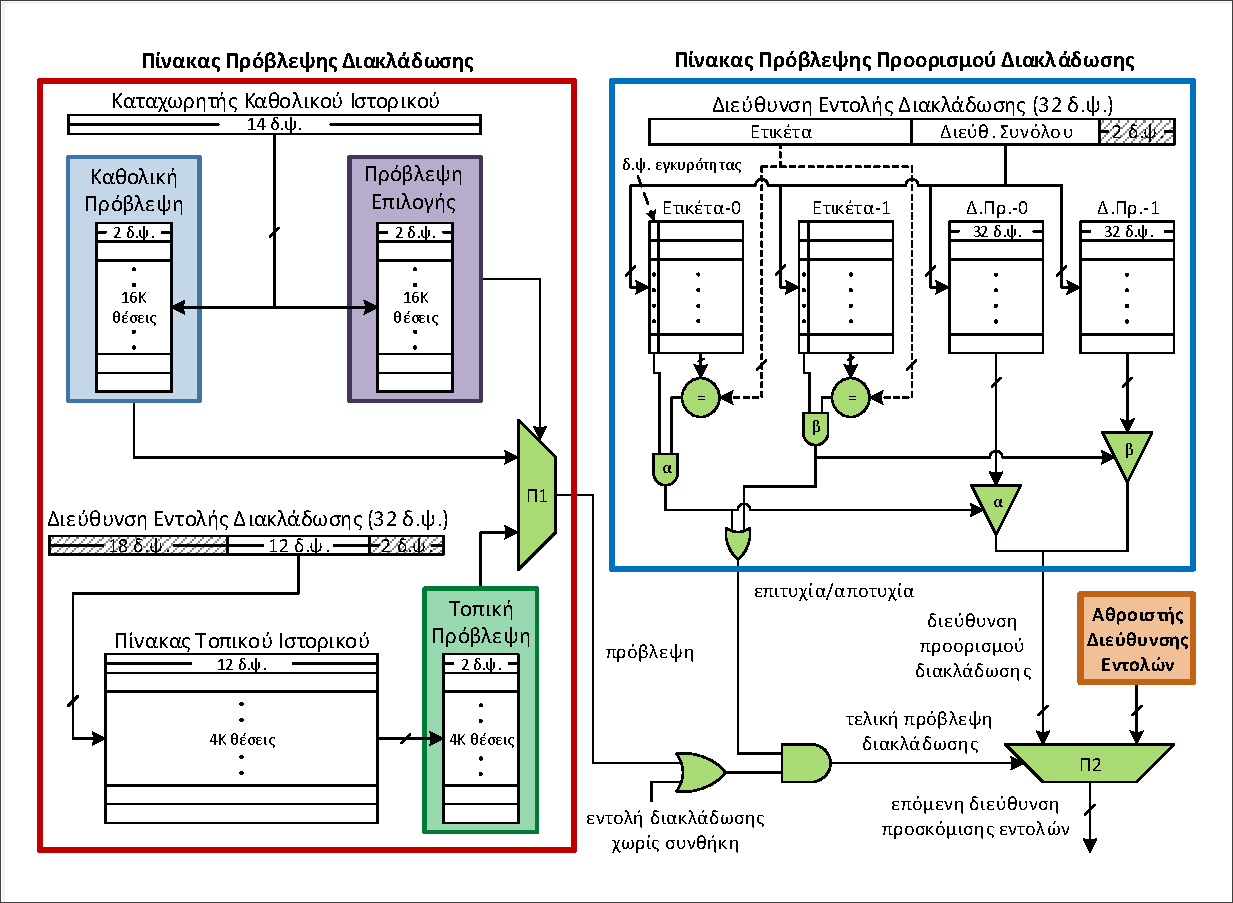
\includegraphics[width=\linewidth, trim=0.5cm 0.8cm 0.5cm 0.8cm, clip=true]{\hardwareDIR/chap2_dynamic_predictor.pdf}}
    \caption{Συνολική δομή της Μονάδας Δυναμικής Πρόβλεψης Διακλαδώσεων}
    \label{fig:chap2_dynamic_predictor}
\end{figure}

Μόλις η εντολή διακλάδωσης εκτελεστεί και αποφανθεί εάν η πρόβλεψη ήταν σωστή ή όχι, γίνεται η κατάλληλη ενημέρωση της αντίστοιχης θέσης του Πίνακα Πρόβλεψης Προορισμού Διακλάδωσης ώστε να ενημερωθεί το πεδίο της διεύθυνσης στην οποία έγινε η μετατόπιση της εκτέλεσης του προγράμματος. Με τον τρόπο αυτό αυξάνεται η λόγος επιτυχίας του την επόμενη φορά που θα προσκομιστεί η ίδια εντολή διακλάδωσης. Ομοίως με τις Κρυφές Μνήμες πρώτου επιπέδου, εξαιτίας του περιορισμένου αριθμού πλαισίων ανά σύνολο απαιτείται η χρήση μίας μεθόδου αντικατάστασης ώστε όταν δεν υπάρχουν διαθέσιμα πλαίσια για την αποθήκευση της κατάλληλης πληροφορίας μίας νέας εντολής διακλάδωσης να πραγματοποιείται αντικατάσταση των δεδομένων μίας δεσμευμένης θέσης. Συνηθισμένη μέθοδος αντικατάστασης είναι αυτή του Λιγότερο Πρόσφατα Χρησιμοποιηθέντος (\en{LRU}) στοιχείου \cite{sudarshan2004highly, al2004performance}, η οποία έχει αποδειχθεί εύκολα υλοποιήσιμη και αρκετά αποδοτική.
\par
Στο Σχήμα \ref{fig:chap2_dynamic_predictor} παρουσιάζεται η συνολική δομή της Μονάδας Δυναμικής Πρόβλεψης Διακλαδώσεων, όπου τα αποτελέσματα των δύο πινάκων οδηγούνται σε κατάλληλες πύλες ώστε να αποφανθεί η διεύθυνση κρυφής μνήμης εντολών από την οποία θα προσκομιστούν οι επόμενες εντολές.

%----------------------------------------------------------%

\subsection{Δειγματοληπτικά Στοιχεία Εντολών Διακλάδωσης}

Η μελέτη της αποδοτικής εξαγωγής προβλέψεων απασχολεί τους ερευνητές από τα πρώτα στάδια ανάπτυξης του υπερβαθμωτού επεξεργαστή. Πολλές μελέτες έχουν επικεντρωθεί στην ανάλυση τους όπως για παράδειγμα τα \cite{Lee2003ExploitingCT} και \cite{eyerman2006characterizing}. Όπως είναι αναμενόμενο, τα μετροπρογράμματα παρουσιάζουν διαφορές στη συμπεριφορά τους. Ορισμένα από αυτά αποτελούνται από αρκετές εντολές διακλάδωσης και επομένως η επιτυχία της Μονάδας Δυναμικής Πρόβλεψης Διακλαδώσεων συμβάλει σημαντικά στην ταχύτερη εκτέλεσή τους.
\par
Το ποσοστό πλήθους και είδους εντολών διακλάδωσης παρουσιάζονται στο Σχήμα \ref{fig:chap2_branch_instr_stats} όπου το άθροισμα των πορτοκαλί και μπλε αποχρώσεων δηλώνει το ποσοστό των εντολών διακλάδωσης σε σχέση με τις συνολικές εντολές που προσκομίζονται, για κάθε μετροπρόγραμμα \spec ξεχωριστά. Οι πορτοκαλί αποχρώσεις αποτελούν ένα τμήμα του συνόλου των εντολών διακλάδωσης και δηλώνουν το ποσοστό αυτών που χρησιμοποιούν τον Πίνακα Πρόβλεψης Προορισμού Διακλάδωσης (ΠΠΠΔ).
\par
Η γραφική παράσταση φανερώνει τις περιπτώσεις μετροπρογραμμάτων οι οποίες θα εκμεταλλευτούν κατά το μέγιστο τον Πίνακα Πρόβλεψης Προορισμού Διακλάδωσης, ο οποίος μελετάται στην παρούσα διπλωματική, και επομένως ο χρόνος εκτέλεσής τους θα εξαρτάται ιδιαίτερα από την ευστοχία του.

\begin{figure}[!h]
    \centering
    \fbox{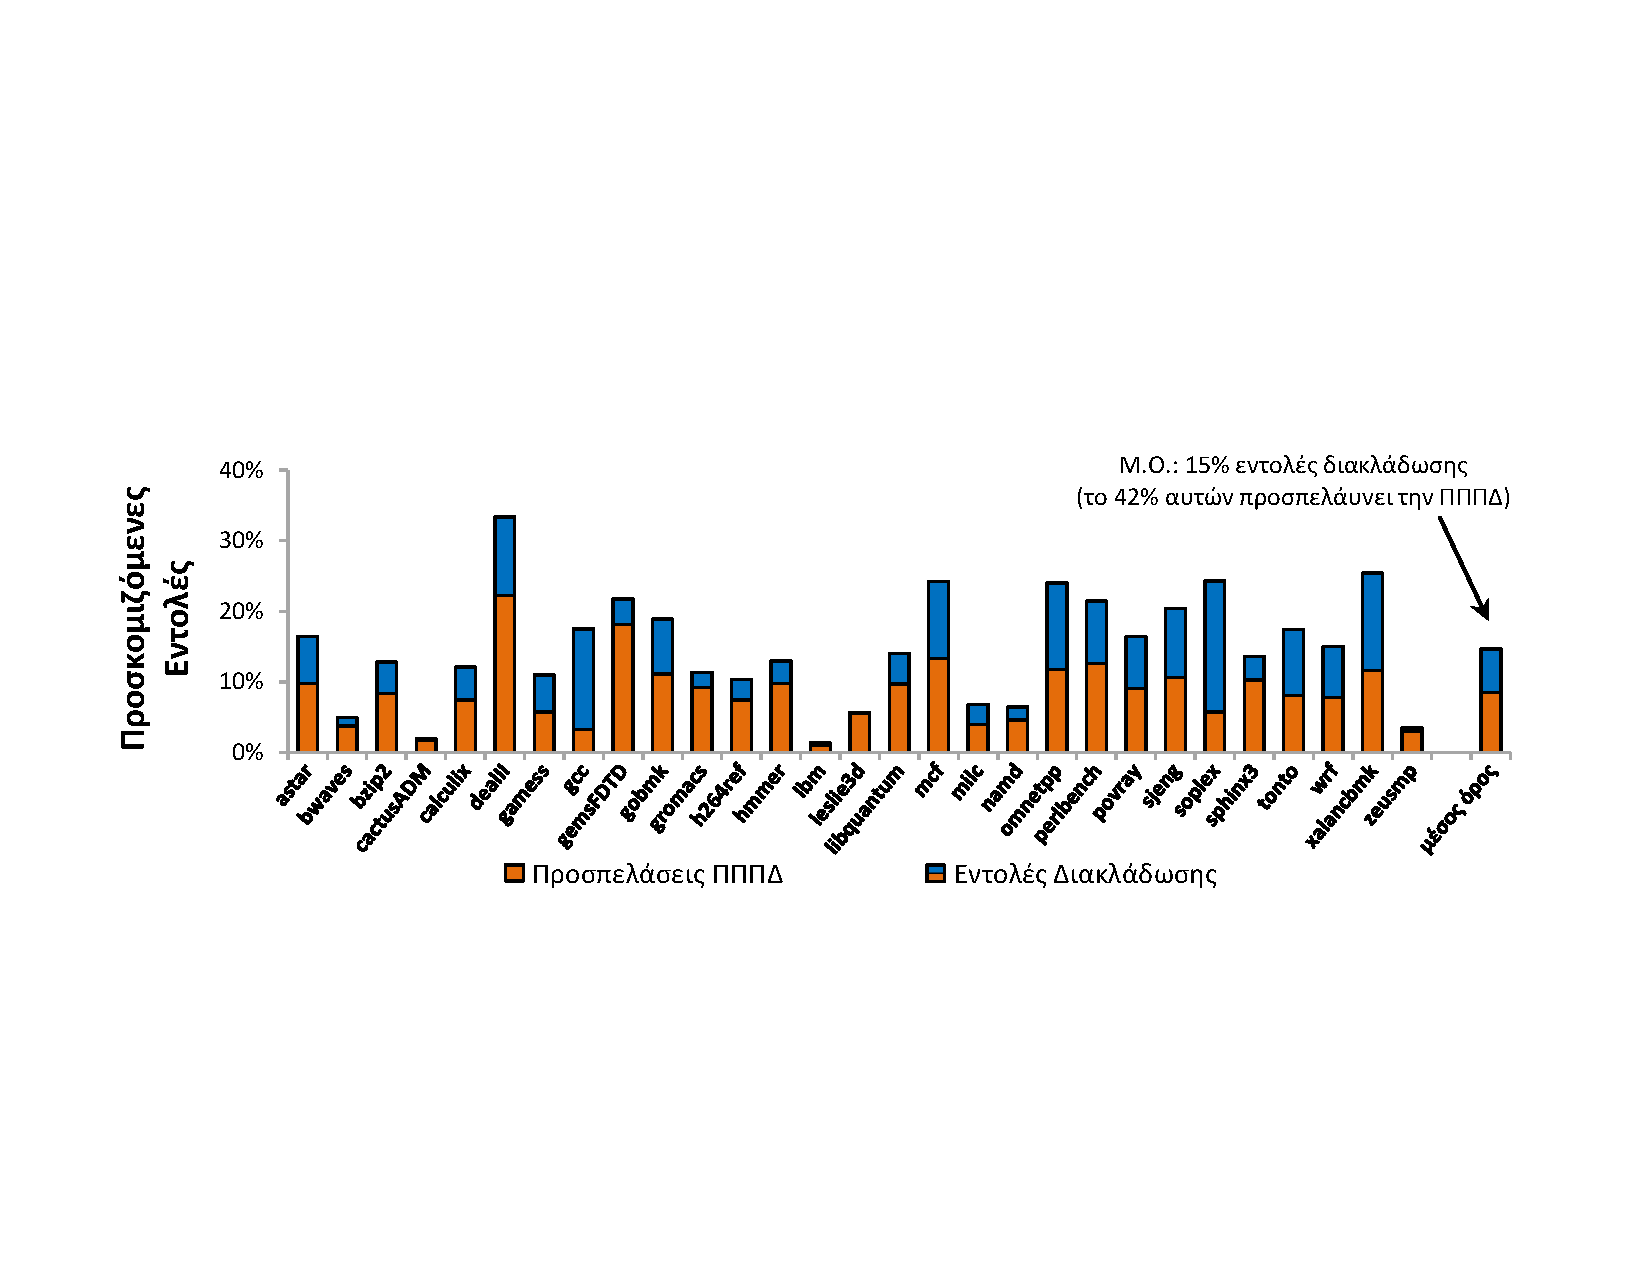
\includegraphics[width=\linewidth, trim=1.9cm 6.5cm 1.8cm 6.6cm, clip=true]{\resultsDIR/chap2_branch_insts.pdf}}
    \caption{Ποσοστό εντολών διακλάδωσης ως προς το σύνολο των προσκομισθέντων εντολών και ποσοστό εντολών διακλάδωσης που προσπελαύνουν τον Πίνακα Πρόβλεψης Προορισμού Διακλάδωσης}
    \label{fig:chap2_branch_instr_stats}
\end{figure}

%----------------------------------------------------------%

    \chapter{Κατανάλωση Ισχύος Ψηφιακών Κυκλωμάτων}
\label{chap3}

\section{Εισαγωγή}
\label{chap3_Intro}

Η επιτακτική ανάγκη συρρίκνωσης των τρανζίστορ σε συνδυασμό με την ταυτόχρονη μείωση της τάσης λειτουργίας τους έχει αναδείξει ένα πολύ σημαντικό ζήτημα στα σύγχρονα ολοκληρωμένα κυκλώματα, αυτό της εμφάνισης βλαβών. Η βλάβη ενός στοιχείου του κυκλώματος μπορεί να έχει ως αποτέλεσμα την καθυστέρηση των υπολογισμών, καθιστώντας το σύστημα μη αποδοτικό, και στη χειρότερη περίπτωση την αλλοίωση των δεδομένων, καθιστώντας το μη αξιόπιστο. Για την αντιμετώπιση αυτών των βλαβών έχουν προταθεί και υλοποιηθεί πληθώρα μεθόδων, με σκοπό τον κατά το δυνατό μεγαλύτερο περιορισμό των επιπτώσεών τους. Στο παρόν κεφάλαιο γίνεται η θεωρητική προσέγγιση της κατανάλωσης ενέργειας των ψηφιακών κυκλωμάτων καθώς και η περιγραφή της σχέσης μεταξύ της εφαρμοζόμενης τάσης λειτουργίας και της πιθανότητας εμφάνισης βλαβών σε αυτά.

%----------------------------------------------------------%

\section{Κατανάλωση Ολοκληρωμένων Κυκλωμάτων}
\label{chap3_LowPowerSOC}

Αποτελεί γεγονός πως η πρόοδος της σχεδίασης των ψηφιακών κυκλωμάτων βαδίζει με γοργούς ρυθμούς. Όπως προέβλεπε ο νόμος του \en{Moore} \cite{moore2006progress} το 1975, το πλήθος των τρανζίστορ ενός ολοκληρωμένου (βαθμός ολοκλήρωσης) θα διπλασιάζεται κάθε δύο χρόνια. Παρότι τα τελευταία χρόνια θεωρήθηκε αρκετές φορές πως ο ρυθμός ολοκλήρωσης πρόκειται σύντομα να επιβραδυνθεί, η σχεδίαση ολοένα και μικρότερου μεγέθους τρανζίστορ συνεχίζει να επιβεβαιώνει το νόμο, καθιστώντας αυτό το στόχο ως κίνητρο έρευνας για τους κατασκευαστές μικροεπεξεργαστών \cite{moore2003no}. Από τα 130\nm – 45\nm μεγέθους τρανζίστορ που παρουσιάστηκαν την δεκαετία του 2000 η τεχνολογία των 14\nm αποτελεί πλέον γεγονός, ενώ οι κατασκευαστές έχουν ήδη ανακοινώσει πως σύντομα θα πραγματοποιηθεί η υλοποίηση τρανζίστορ μεγέθους 10\nm \cite{courtland2017moore}.
\par
Η ιλιγγιώδης αύξηση του πλήθους τρανζίστορ που εμπεριέχονται σε έναν επεξεργαστή (2-4 δισεκατομμύρια τρανζίστορ) είχε ώς συνέπεια τη μεγάλη αύξηση της καταναλισκόμενης ενέργειας και της εκλυόμενης θερμότητας, με τις συνέπειες που αυτή έχει στην ορθή λειτουργία των στοιχείων του. Στο γράφημα του Σχήματος \ref{fig:chap3_energy_per_tech} παρουσιάζεται τμήμα του άρθρου του \en{Dreslinski} και άλλων \cite{dreslinski2010near}, σχετικά με την εξέλιξη των ολοκληρωμένων κυκλωμάτων τα τελευταία χρόνια. Στο συγκεκριμένο γράφημα η καμπύλη μαύρου χρώματος αντιστοιχεί στη συνολική κατανάλωση ενέργειας του κυκλώματος (άξονας αριστερά). Τα δεδομένα παρουσιάζονται κανονικοποιημένα ως προς την περίπτωση κυκλώματος τεχνολογίας 250\nm. Στα πρώτα στάδια η μείωση του μεγέθους αποτέλεσε πολύ σημαντικό παράγοντα στην προσπάθεια περιορισμού της απώλειας ενέργειας. Όπως φαίνεται και από το γράφημα, η μετάβαση από τα 250\nm στο 180\nm προκάλεσε μείωση της καταναλισκόμενης ενέργειας πάνω από 50\%. Παρόλα αυτά, ο ρυθμός μείωσης της κατανάλωσης παρουσιάζει πτωτική τάση καθώς το μέγεθος των τρανζίστορ τείνει σε μερικές δεκάδες νανόμετρα.

\begin{figure}[!t]
    \centering
    \begin{subfigure}[t]{0.49\textwidth}
        \centering
        \fbox{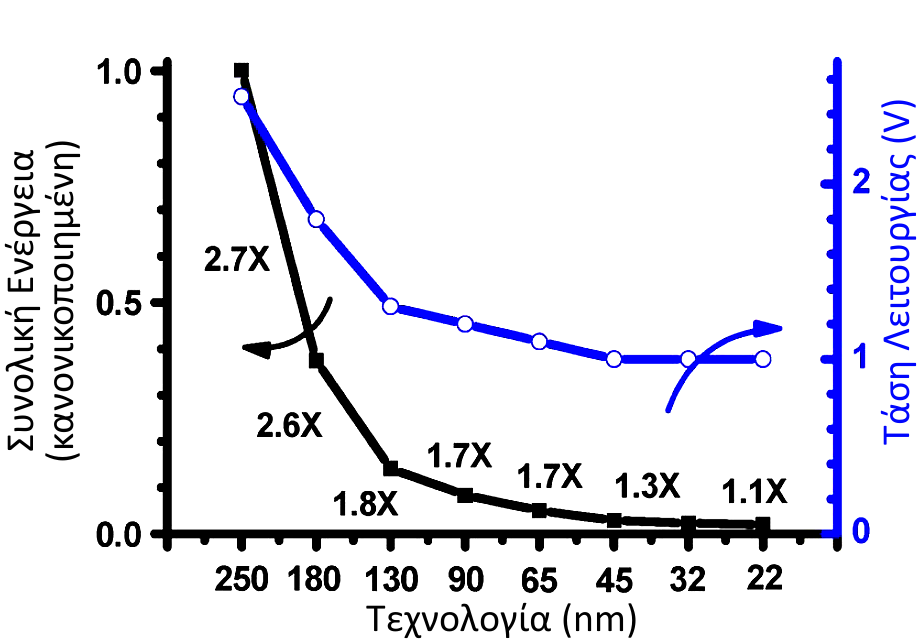
\includegraphics[width=0.98\linewidth, clip=true]{\researchesDIR/chap3_tech_energy.png}}
        \caption[Συνολική ενέργεια $\&$ τάση λειτουργίας]{Συνολική ενέργεια $\&$ τάση λειτουργίας \cite{dreslinski2010near}}
        \label{fig:chap3_energy_per_tech}
    \end{subfigure}%
    \hfill
    \begin{subfigure}[t]{0.49\textwidth}
        \centering
        \fbox{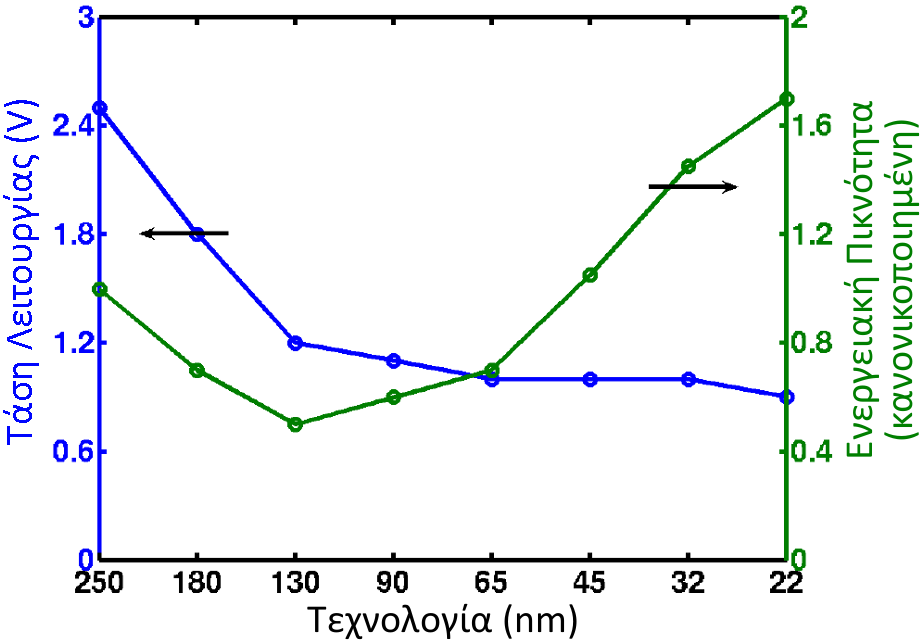
\includegraphics[width=0.98\linewidth, clip=true]{\researchesDIR/chap3_tech_vdd_ed.png}}
        \caption[Τάση λειτουργίας $\&$ πυκνότητα ενέργειας]{Τάση λειτουργίας $\&$ πυκνότητα ενέργειας \cite{pinckney2012assessing}}
        \label{fig:chap3_vdd_per_tech}
    \end{subfigure}
    \caption{Μεταβολή της τάσης λειτουργίας και της ενέργειας με τη συρρίκνωση της τεχνολογίας. Τα αποτελέσματα της συνολικής ενέργειας και της πυκνότητας ενέργειας εμφανίζονται κανονικοποιημένα ως προς τη περίπτωση των 250\nm.}
    \label{fig:chap3_Technology}
\end{figure}

Όπως αναφέρει και η μελέτη του \en{Pinckney} και άλλων \cite{pinckney2012assessing}, η αύξηση των ρευμάτων διαρροής των τρανζίστορ κατέστησε αδύνατη τη μείωση της τάσης κατωφλίου από το σημείο των 65\nm και έπειτα, επομένως και τη μείωση της τάσης λειτουργίας του κυκλώματος, όπως φανερώνει και η καμπύλη μπλε απόχρωσης στα Σχήματα \ref{fig:chap3_energy_per_tech} και \ref{fig:chap3_vdd_per_tech}. Η αδυναμία περαιτέρω μείωσης της τάσης λειτουργίας σε συνδυασμό με τη συνεχόμενη αύξηση της κλίμακας ολοκλήρωση έχει ως αποτέλεσμα την αύξηση της πυκνότητας ενέργειας, δηλαδή της ενέργειας που δαπανάται ανά τετραγωνικό χιλιοστό (καμπύλη πράσινης απόχρωσης Σχήματος \ref{fig:chap3_vdd_per_tech}). Αυτή η αύξηση συνεπάγεται την υπερθέρμανση ορισμένων κρίσιμων τμημάτων του ολοκληρωμένου, με κίνδυνο εμφάνισης βλαβών σε αυτά μελλοντικά. Η κατανάλωση ισχύος ενός κυκλώματος (κατανάλωση ενέργειας στο χρόνο) οφείλεται σε μία πληθώρα στοιχείων, και μπορεί να διαχωριστεί σε δύο βασικές κατηγορίες:
\par
\textit{\textbf{Δυναμική:}} Η ισχύς που καταναλώνεται όταν ένας κόμβος (τρανζίστορ) του κυκλώματος πραγματοποιεί μετάβαση κατάστασης από 0 σε 1 και αντίστροφα. Όταν στο κύκλωμα εφαρμόζεται η ονομαστική τάση λειτουργίας οι καταναλώσεις αυτού του είδους αποτελούν τον πιο σημαντικό παράγοντα στη συνολική κατανάλωση ισχύος του συστήματος.
\par
\textit{\textbf{Στατική:}} Η ισχύς που καταναλώνεται σε ένα κύκλωμα όταν δεν πραγματοποιείται μεταβολή της κατάστασής στους κόμβους (τρανζίστορ) του, και οφείλεται στα ρεύματα διαρροής των τρανζίστορ. Καθώς η τεχνολογία συρρικνώνεται και η τάση λειτουργίας μειώνεται οι καταναλώσεις αυτού του είδους αποτελούν πολύ σημαντικό παράγοντα στη συνολική κατανάλωση ισχύος, σχεδόν όσο και η δυναμική.\par
\par

\begin{figure}[!t]
    \centering
    \begin{subfigure}[t]{0.49\textwidth}
        \centering
        \fbox{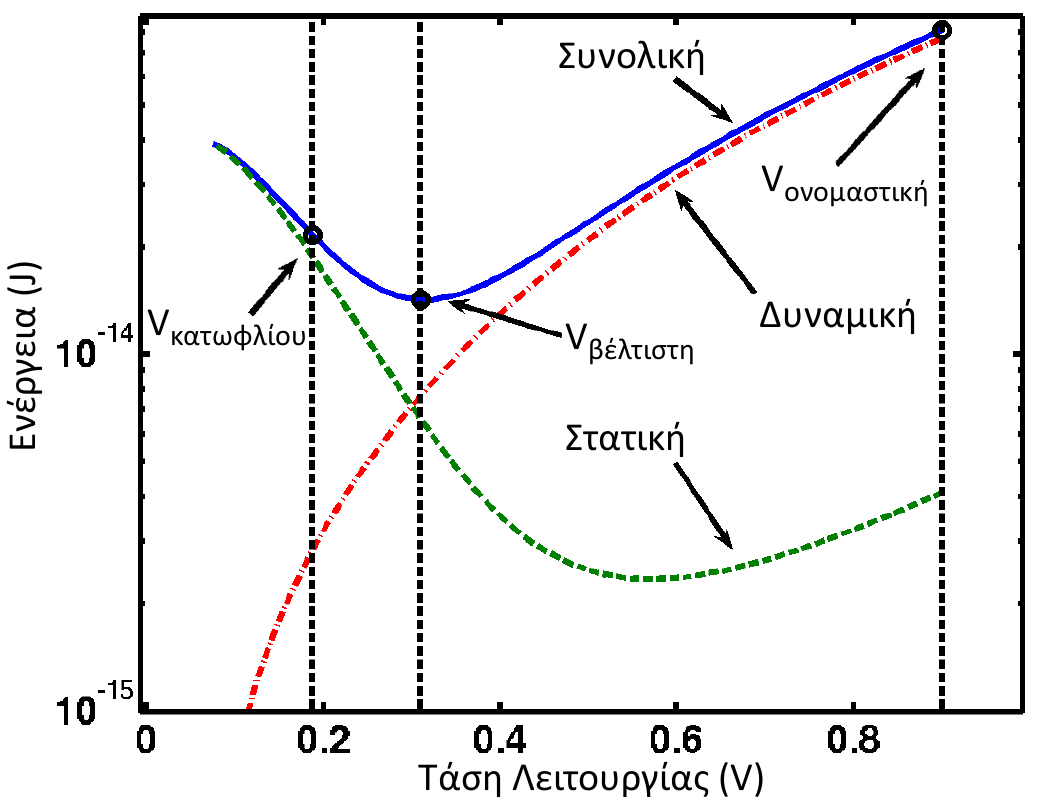
\includegraphics[width=0.98\linewidth, clip=true]{\researchesDIR/chap3_vdd_energy.png}}
        \caption{Συνολική, δυναμική $\&$ στατική κατανάλωση}
        \label{fig:chap3_energy_per_vdd}
    \end{subfigure}%
    \hfill
    \begin{subfigure}[t]{0.49\textwidth}
        \centering
        \fbox{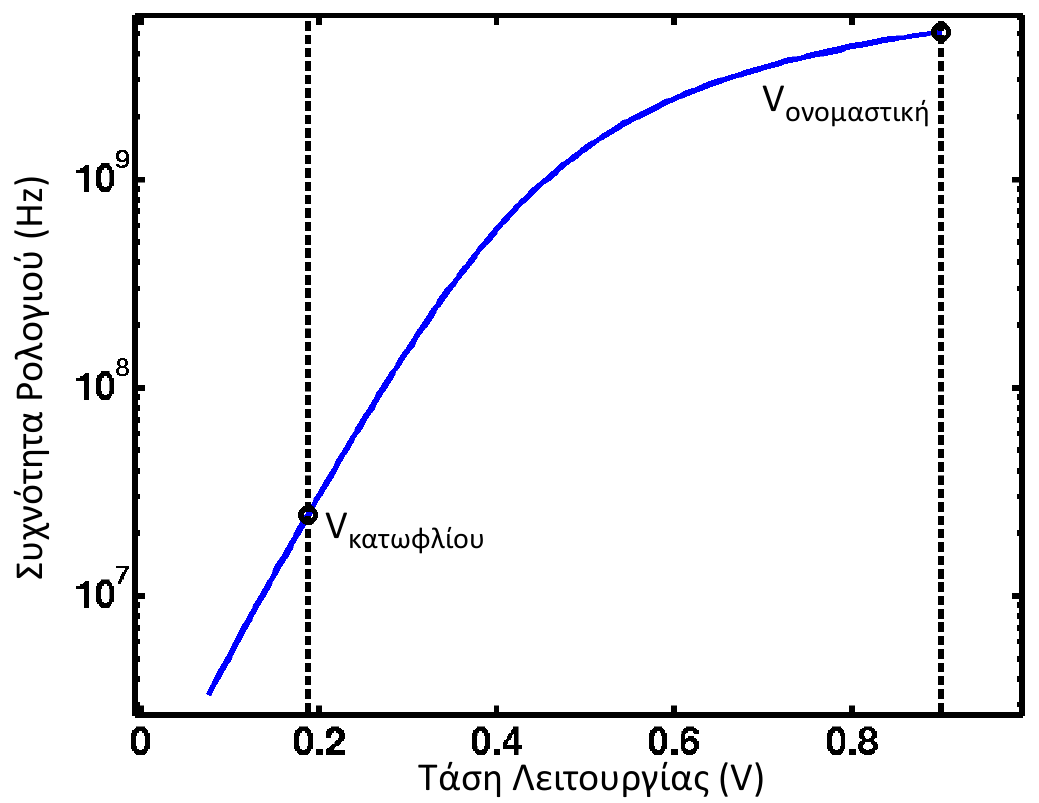
\includegraphics[width=0.98\linewidth, clip=true]{\researchesDIR/chap3_vdd_freq.png}}
        \caption{Μέγιστη συχνότητα λειτουργίας}
        \label{fig:chap3_freq_per_vdd}
    \end{subfigure}
    \caption[Μεταβολή της καταναλισκόμενης ενέργειας και της μέγιστης συχνότητας ρολογιού σε διαφορετικές τάσεις λειτουργίας ενός κυκλώματος τεχνολογίας 32\nm]{Μεταβολή της καταναλισκόμενης ενέργειας και της μέγιστης συχνότητας ρολογιού σε διαφορετικές τάσεις λειτουργίας ενός κυκλώματος τεχνολογίας 32\nm \cite{pinckney2012assessing}}
    \label{fig:chap3_Vdd}
\end{figure}

Στο γράφημα του Σχήματος \ref{fig:chap3_energy_per_vdd} παρουσιάζεται η σχέση μεταξύ δυναμική και στατικής κατανάλωσης για διαφορετικά επίπεδα τάσης λειτουργίας ενός ολοκληρωμένου τεχνολογίας 32\nm, όπως αναφέρεται στην ίδια μελέτη του \en{Pinckney} \cite{pinckney2012assessing}. Αντίστοιχα, το γράφημα του Σχήματος \ref{fig:chap3_freq_per_vdd} παρουσιάζει τη μεταβολή της συχνότητας σε αυτό το εύρος τάσης. Από το πρώτο γράφημα γίνεται ξεκάθαρο πως με τη μείωση της τάσης λειτουργίας έως το βέλτιστο σημείο η συνολική κατανάλωση ενέργειας μειώνεται (καμπύλη μπλε απόχρωσης). Χαρακτηριστικό είναι το γεγονός πως για τάση λειτουργίας μικρότερη του βέλτιστου παρουσιάζεται σημαντική αύξηση της στατικής κατανάλωσης (καμπύλη πράσινης απόχρωσης), σε αντίθεση με τη δυναμική (καμπύλη κόκκινης απόχρωσης) η οποία συνεχώς μειώνεται. Στο σημείο που η στατική κατανάλωση ισούται με τη δυναμική η τάση λειτουργίας αποτελεί τη βέλτιστη επιλογή για τη μείωση της συνολικής καταναλισκόμενης ενέργειας. Παράλληλα, με τη μείωση της τάσης λειτουργίας αναπόφευκτα επιβάλλεται και η πτώση της συχνότητας ρολογιού εξαιτίας της αύξησης του χρόνου εναλλαγής καταστάσεων των τρανζίστορ. Η μείωση αυτή παρουσιάζεται στο δεύτερο γράφημα (Σχήμα \ref{fig:chap3_freq_per_vdd}).

%----------------------------------------------------------%

\section{Δυναμική Μεταβολή Τάσης και Συχνότητας}
\label{chap3_PowerReduction}

Ο σχεδιασμός ενός συστήματος μειωμένης κατανάλωσης μπορεί τα επιτευχθεί μέσω του συνδυασμού κατάλληλων τεχνικών στα διαφορετικά επίπεδα που το αποτελούν. Ξεκινώντας από το χαμηλότερο επίπεδο, αυτό της σχεδίασης ψηφιακών κυκλωμάτων, έως και το ανώτερο επίπεδο, της σχεδίασης του λογισμικού που εκτελείται στο κύκλωμα, είναι αναγκαίο να επιτυγχάνεται η αύξηση της απόδοσης με ταυτόχρονη μείωση του κόστους που έχει σε ενέργεια. Από τις μελέτες που παρουσιάστηκαν αλλά και πολλές ακόμη που έχουν διενεργηθεί τα τελευταία χρόνια σε επίπεδο υλικού, προκύπτει πως για να επιτευχθεί η μείωση της καταναλισκόμενης ενέργειας ενός ολοκληρωμένου κυκλώματος απαιτείται η εφαρμογή κατάλληλου συνδυασμού τάσης και συχνότητας λειτουργίας \cite{zhai2009energy, lorente2014analyzing, de2016near}. Το γεγονός αυτό εκμεταλλεύονται οι σύγχρονοι υπερβαθμωτοί επεξεργαστές οι οποίοι σχεδιάζονται κατά τέτοιο τρόπο ώστε να μπορούν να λειτουργούν σε διαφορετικά επίπεδα τάσης και συχνότητας ανά χρονικά διαστήματα. Η τεχνική αυτή ονομάζεται Δυναμική Μεταβολή Τάσης και Συχνότητας (\en{DVFS}) και αποτελεί πλέον αναπόσπαστο κομμάτι τους.
\par
Η ιδέα του \en{DVFS} βασίζεται στο γεγονός ότι ο φόρτος εργασίας μεταβάλλεται κατά το χρόνο λειτουργίας ενός επεξεργαστή. Επομένως, στις χρονικές περιόδους όπου η απαιτούμενη επεξεργαστική ισχύς είναι μικρή μπορεί να γίνει υποβάθμιση της απόδοσης του συστήματος ώστε να μειωθεί η δυναμική κατανάλωση του, η οποία υπολογίζεται από τη σχέση:

\begin{equation}
    \label{eqn:chap3_dynamic_power}
    P = CV^{2}f
\end{equation}

\noindent
όπου $C$ είναι η συνολική χωρητικότητα του κυκλώματος, $V$ η τάση λειτουργίας, και $f$ η συχνότητα ρολογιού.
\par
Στη σχέση \eqref{eqn:chap3_dynamic_power} η χωρητικότητα αποτελεί σταθερό παράγοντα ενός κυκλώματος, εν αντιθέσει με τη τάση και τη συχνότητα τα οποία μπορούν να μεταβάλλονται. Συνεπώς, για να επιτευχθεί η μείωση της κατανάλωσης ισχύος πρέπει να γίνει κατάλληλη προσαρμογή των παραγόντων τάση και συχνότητα. Όπως είναι φανερό, μία μικρή μείωση της τάσης λειτουργίας μπορεί να οδηγήσει σε σημαντική μείωση της δυναμικής κατανάλωσης ισχύος. Στο γράφημα του Σχήματος \ref{fig:chap3_intel_ntv} παρουσιάζεται η μεταβολή της συχνότητας και της κατανάλωσης ισχύος ενός επεξεργαστή τεχνολογίας 32\nm, για διαφορετικά επίπεδα τάσης λειτουργίας, όπως παρουσιάζονται στο άρθρο των \en{De}, \en{Vangal} και \en{Krishnamurthy} \cite{de2016near}.

\begin{figure}[h]
    \centering
    \fbox{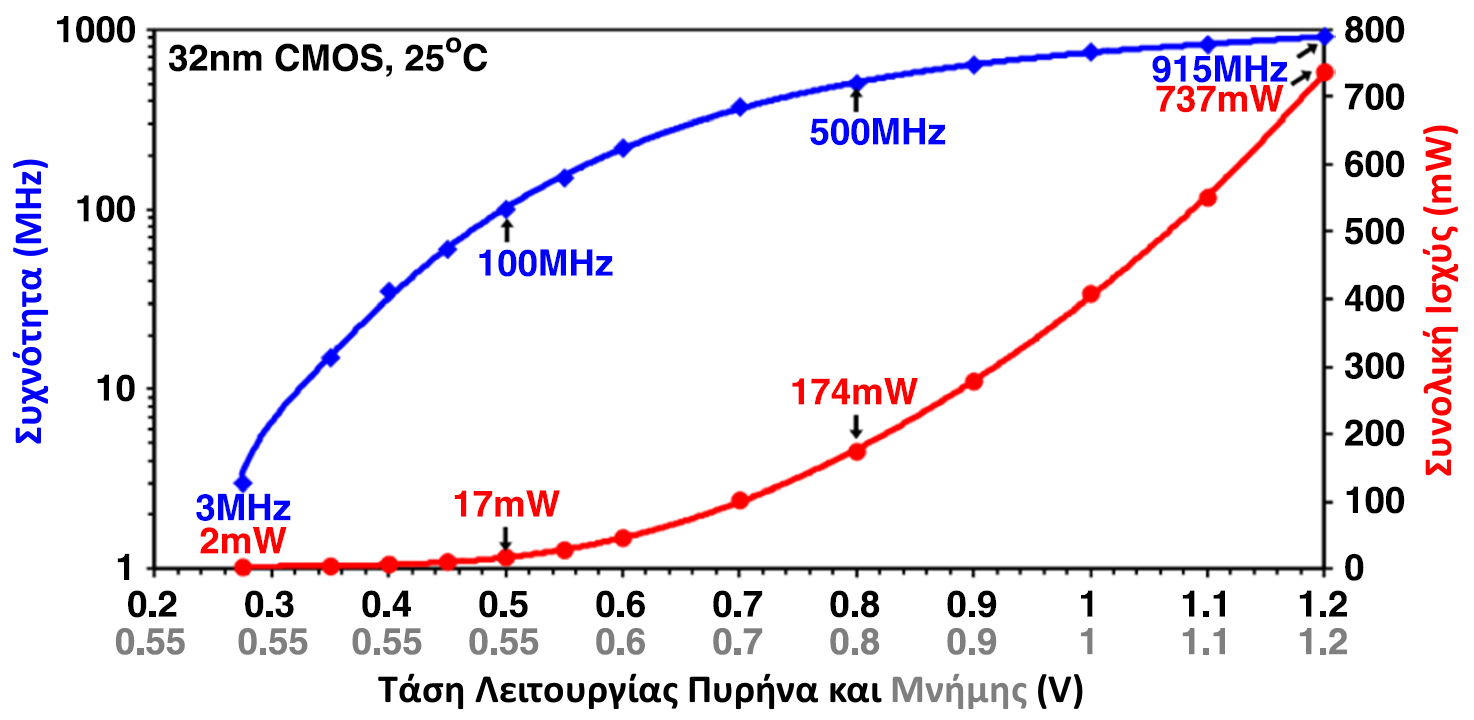
\includegraphics[width=0.85\linewidth, clip=true]{\researchesDIR/chap3_intel_ntv.png}}
    \caption[Σχέση συχνότητας και ισχύος με τις μεταβολές του επιπέδου τάσης λειτουργίας ενός επεξεργαστή τεχνολογίας 32\nm]{Σχέση συχνότητας και ισχύος με τις μεταβολές του επιπέδου τάσης λειτουργίας ενός επεξεργαστή τεχνολογίας 32\nm \cite{de2016near}}
    \label{fig:chap3_intel_ntv}
\end{figure}

%----------------------------------------------------------%

\section{Δυναμικό Χαμηλού Επιπέδου και Βλάβες}
\label{chap3_LowLevelVccFaults}

Όπως αναφέρθηκε ήδη, η συρρίκνωση του μεγέθους των τρανζίστορ σε συνδυασμό με την αύξηση της ολοκλήρωσης των επεξεργαστών οδηγεί στην εμφάνιση βλαβών. Ιδιαίτερα, καθώς η τάση λειτουργίας των τρανζίστορ μειώνεται σημαντικά σε σχέση με την ονομαστική, με σκοπό τη μείωση της κατανάλωσης κατά το μέγιστο δυνατόν, ορισμένα από αυτά αρχίζουν να μην λειτουργούν με τον αναμενόμενο τρόπο. Τα πιο συνηθισμένα «θύματα» αυτής της μεγάλης μείωσης της τάσης λειτουργίας είναι οι κυψελίδες \en{SRAM} που αποτελούν τα στοιχεία μνήμης του ολοκληρωμένου. Εξαιτίας της μεγάλης επιφάνειας που καταλαμβάνουν τα στοιχεία μνήμης, συνηθίζεται να υλοποιούνται με μικρότερα και συνεπώς πιο ευάλωτα τρανζίστορ \cite{nassif2010resilience, gottscho2014power}. Αυτό έχει σαν συνέπεια να παρουσιάζουν είτε αστάθεια στη συμπεριφορά τους είτε να μην ανταποκρίνονται καθόλου σε επιθυμητές μεταβολές της κατάστασής τους. Στο Σχήμα \ref{fig:chap3_22nm_pfail} παρουσιάζεται τμήμα της μελέτης της \en{Ferreron} και άλλων \cite{ferreron2014block}, και όπως φανερώνει το γράφημα, η πιθανότητα μίας κυψελίδας \en{SRAM} να εμφανίσει βλάβη αυξάνεται μη γραμμικά καθώς η τάση λειτουργίας μειώνεται.

\begin{figure}[h]
    \centering
    \fbox{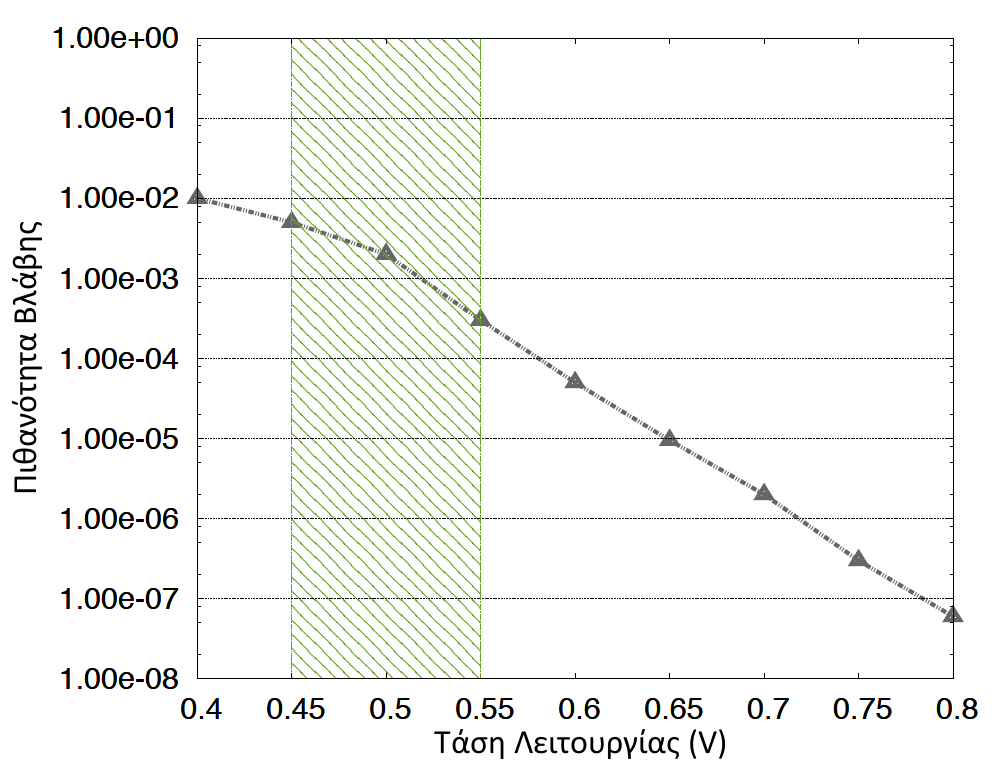
\includegraphics[width=0.7\linewidth, clip=true]{\researchesDIR/chap3_pfail_vdd_22nm.png}}
    \caption[Μεταβολή της πιθανότητα βλάβης μίας \en{SRAM} κυψελίδας στα 22\nm με τη μεταβολή της τάσης λειτουργίας]{Μεταβολή της πιθανότητα βλάβης μίας \en{SRAM} κυψελίδας στα 22\nm με τη μεταβολή της τάσης λειτουργίας \cite{ferreron2014block}}
    \label{fig:chap3_22nm_pfail}
\end{figure}

Με τη συρρίκνωση της τεχνολογίας η καμπύλη αυτή μετατοπίζεται προς τα επάνω, διότι τα τρανζίστορ γίνονται περισσότερο ευάλωτα. Όταν μία κυψελίδα περιέχει βλάβη χαρακτηρίζεται ως ελαττωματική, και τα δεδομένα που αποθηκεύονται σε αυτή αυτή είναι πιθανό να αλλοιωθούν. Επομένως, οι ελαττωματικές αυτές θέσεις ενός ολοκληρωμένου χαρακτηρίζονται ως σφάλματα \cite{nikolosTesting}.

%----------------------------------------------------------%

\section{Ανίχνευση/Διόρθωση Λαθών και Ανοχή Σφαλμάτων}
\label{chap3_FaultTaulerance}

Για την αντιμετώπιση των σφαλμάτων του συστήματος, τόσο κατά την κατασκευή όσο και κατά τη λειτουργία του, πραγματοποιείται κατάλληλος έλεγχος ώστε να εντοπίζονται εάν και σε ποια σημεία του κυκλώματος εμφανίζονται λάθη. Η διαδικασία αυτή αποκαλείται Ανίχνευση Σφαλμάτων και σε αρκετά συστήματα η εκτέλεσή της πραγματοποιείται σε διαφορετικά στιγμιότυπα της λειτουργίας τους.
\par
Η εμφάνιση σφαλμάτων μπορεί να οδηγήσει είτε σε απλή επιβάρυνση του χρόνου εκτέλεσης των προγραμμάτων (μείωση της απόδοσης), το οποίο θα έχει και ως συνέπεια την αύξηση της καταναλισκόμενης ενέργειας, είτε την παραγωγή λανθασμένων αποτελεσμάτων. Στην πρώτη περίπτωση, παρότι η σωστή εκτέλεση του προγράμματος δεν τίθεται σε κίνδυνο, χρησιμοποιούνται κατάλληλες τεχνικές ώστε να περιορίζεται η επιβάρυνση της απόδοσης κατά το μέγιστο δυνατόν. Αντιθέτως, στη δεύτερη περίπτωση η μη αντιμετώπιση των ελαττωματικών στοιχείων μνήμης θα οδηγούσε σε υλοποίηση ενός μη αξιόπιστου επεξεργαστικού στοιχείου. Για το λόγο αυτό, εάν κρίνεται απαραίτητο χρησιμοποιούνται κατάλληλες τεχνικές Διόρθωσης Λαθών. Εξαιτίας του υψηλού κόστους των τεχνικών αυτών αλλά και των πεπερασμένων λύσεων που προσφέρουν καθώς αυξάνεται το πλήθος των σφαλμάτων, η απενεργοποίηση των ελαττωματικών στοιχείων αποτελεί μονόδρομος σε πολλές περιπτώσεις, ώστε να μην επηρεάζεται η συνολική λειτουργία του συστήματος.
\par
Ώς Ανοχή Σφαλμάτων αναφέρεται η δυνατότητα ενός συστήματος να είναι σε θέση να λειτουργεί σωστά παρά την ύπαρξη σφαλμάτων. Συνηθισμένη τακτική για την περίπτωση των μνημών είναι η απενεργοποίηση των κυψελίδων αυτών, ώστε ούτε να αλλοιώνονται τα δεδομένα που αποθηκεύονται σε αυτές ούτε να επιβαρύνουν το κύκλωμα με περιττή σπατάλη ενέργειας για τη λειτουργία τους \cite{wilkerson2008trading, koren2010fault}. Πληθώρα μελετών έχουν παρουσιαστεί τα τελευταία χρόνια στις οποίες προτείνονται κατάλληλες τεχνικές για την αντιμετώπιση των επιπτώσεων που προκύπτουν εξαιτίας των σφαλμάτων στις κρυφές μνήμες, όπως τα \cite{wilkerson2008trading, shirvani1999padded, ansari2009zerehcache, koh2009salvage, lee2011defcam, choi2011matching, keramidas2014spatial, mavropoulos2015defect}. Αντιθέτως, έως τώρα δεν έχει αναπτυχθεί κάποια αντίστοιχη τεχνική για την αντιμετώπιση των πιθανών σφαλμάτων που προκύπτουν στα στοιχεία μνήμης της Μονάδας Δυναμικής Πρόβλεψης Διακλαδώσεων.
\par
Στο επόμενο κεφάλαιο αναλύεται η εμφάνιση ελαττωματικών κυψελίδων στα στοιχεία που αποτελούν τη Μονάδα Δυναμικής Πρόβλεψης Διακλαδώσεων, η λειτουργίας της οποία παρουσιάστηκε στο Κεφάλαιο \ref{chap2}, και αναδεικνύονται οι επιπτώσεις που έχουν στην απόδοση του υπερβαθμωτού επεξεργαστή.

%----------------------------------------------------------%

    \chapter{Προβλέψεις Διακλαδώσεων με Σφάλματα}
\label{chap4}

\section{Εισαγωγή}
\label{chap4_Intro}

Όπως έχει αποδειχθεί από πληθώρα ερευνητικών εργασιών, τα στοιχεία μνήμης είναι επιρρεπή σε βλάβες όταν η τάση λειτουργίας που εφαρμόζεται σε αυτές είναι πολύ-χαμηλού επιπέδου. Βασική αιτία είναι η χρήση μικρού μεγέθους κυψελίδων (συνήθως \en{6T SRAM}), ώστε να καταλαμβάνουν όσο το δυνατόν μικρότερο εμβαδόν.
\par
Η Μονάδα Δυναμικής Πρόβλεψης Διακλαδώσεων αποτελείται από ένα σύνολο κυψελίδων μνήμης και επομένως αναμένεται ορισμένα από αυτά να μην λειτουργούν σωστά όταν η τάση λειτουργίας μειώνεται, προκαλώντας έτσι μείωση στην απόδοσης του συστήματος. Σύμφωνα με τη λειτουργία της μονάδας, όπως παρουσιάστηκε στην Ενότητα \ref{chap2_DynamicBranchPredictionUnit}, η ορθή εκτέλεση ενός προγράμματος δεν θα επηρεαστεί καθώς η Μονάδα Δυναμικής Πρόβλεψης Διακλαδώσεων παρέχει απλώς μία πρόβλεψη, η οποία στη χειρότερη περίπτωση θα είναι λανθασμένη και σε μελλοντικό χρόνο θα ανιχνευθεί. Συνεπώς η διόρθωσή τους δεν κρίνεται απαραίτητη. Στο παρόν κεφάλαιο μελετάται η επιβάρυνση που πιθανός θα προκαλέσουν τα σφάλματα αυτά στη συνολική απόδοση του συστήματος, και συνεπώς στην κατανάλωσή του. Ο υπολογισμός της μείωσης της απόδοσης, δηλαδή του ρυθμού ολοκλήρωσης εντολών (\ipc), εξαιτίας της ύπαρξης σφαλμάτων υπολογίζεται ώς:

\begin{equation}
    \label{eqn:chap4_IPCfaulty}
    \mathgr{Μείωση}\_IPC = \frac{IPC_\mathgr{χωρίς\_σφάλματα} - IPC_\mathgr{με\_σφάλματα}}{IPC_\mathgr{χωρίς\_σφάλματα}}
\end{equation}

Τα αποτελέσματα που παρουσιάζονται εξήχθησαν από τον εξομοιούμενο \en{x86} επεξεργαστή για διαφορετικές παραμετροποιήσεις του. Αναλυτικές πληροφορίες για το βασικό μοντέλο επεξεργαστή καθώς και για τη διαδικασία εξομοίωσης περικλείονται στα Κεφάλαια \ref{chap6} και \ref{chap7} αντίστοιχα.

%----------------------------------------------------------%

\section{Σφάλματα στη Μονάδα Δυναμικής Πρόβλεψης Διακλαδώσεων}
\label{chap4_DynamicBranchPredictionUnitFaults}

Σύμφωνα με την έως τώρα ανάλυση, η πολύ μεγάλη μείωση της τάσης λειτουργίας αναμένεται να έχει επιπτώσεις στη Μονάδα Δυναμικής Πρόβλεψης Διακλαδώσεων, προκαλώντας την αύξηση του χρόνου ολοκλήρωσης των προγραμμάτων. Οι μελέτες \cite{hsieh2009tolerance} και \cite{hardy2012performance} επικεντρώνεται στα σφάλματα μόνιμης τιμής μίας μονάδα πρόβλεψης τύπου \en{gshare}. Επίσης, στην \cite{foutris2013ssing} αναλύονται τα σφάλματα μόνιμης τιμής στα στοιχεία που χρησιμοποιούνται αποκλειστικά για την ενίσχυση της απόδοσης, όπως είναι και η μονάδα πρόβλεψης τύπου \en{bimodal} που χρησιμοποιείται. Αντιθέτως, η συγκεκριμένη μελέτη επικεντρώνεται στην εμφάνιση τόσο μόνιμων όσο και προσωρινών σφαλμάτων σε μία μονάδα πρόβλεψης επιλεκτικής διάταξης (\en{tournament}).
\par
Για τη μοντελοποίηση των ελαττωματικών κυψελίδων μνήμης ώς σφάλματα στη Μονάδας Δυναμικής Πρόβλεψης Διακλαδώσεων, παρήχθησαν χάρτες σφαλμάτων για κάθε πιθανότητα σφάλματος στην αντίστοιχη τάση λειτουργίας. Τα σφάλματα θεωρούνται ομοιόμορφα κατανεμημένα στις κυψελίδες της μνήμης και ξεκινώντας από τη μηδενική πιθανότητα σφάλματος (ονομαστική τάση λειτουργίας), σταδιακά αυξάνεται (μείωση της τάσης λειτουργίας) εισάγοντας τα αντίστοιχα πρόσθετα σφάλματα. Επομένως, ο χάρτης σφαλμάτων για την πιθανότητα σφάλματος $2N$ θα περιέχει τα σφάλματα του χάρτη της πιθανότητας σφάλματος $N$ καθώς και κάποια επιπλέον ώστε τα συνολικά σφάλματα να είναι διπλάσια, όπως φαίνεται και από το παράδειγμα του Σχήματος \ref{fig:chap4_fmap_creation}.

\begin{figure}[ht]
    \centering
    \fbox{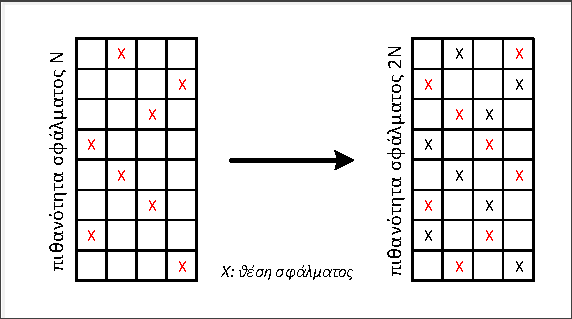
\includegraphics[trim=0.7cm 0.6cm 0.5cm 0.6cm, clip=true]{\hardwareDIR/chap4_fault_maps.pdf}}
    \caption{Δημιουργία χάρτη σφαλμάτων διπλάσιας πιθανότητας σφάλματος}
    \label{fig:chap4_fmap_creation}
\end{figure}

Το συνολικό πλήθος σφαλμάτων που θα περιέχει ένας χάρτης σε κάθε περίπτωση υπολογίζεται από την ακόλουθη σχέση:
\begin{equation}
    \textit{Πλήθος Σφαλμάτων} = \textit{Πιθανότητα Σφάλματος} \times \textit{Πλήθος Κυψελίδων Μνήμης}
\end{equation}

Σύμφωνα με τη μελέτη του \en{Sanchez} και άλλων \cite{sanchez2011analytical}, για την πραγματοποίηση μεγαλύτερης ακρίβειας μετρήσεων οι οποίες βασίζονται σε χάρτες σφαλμάτων πρέπει να εξεταστούν από 100 έως 1000 διαφορετικοί χάρτες. Ο λόγος που απαιτείται αυτός ο μεγάλος αριθμός διαφορετικών χαρτών είναι η ανομοιογένεια των προσπελάσεων στα σύνολα της μνήμης μεταξύ των μετροπρογραμμάτων. Επομένως πραγματοποιήθηκαν 100 επαναλήψεις της διαδικασίας παραγωγής χαρτών σφαλμάτων, για διαφορετικές πιθανότητες. Το πλήθος αυτό θεωρείται ικανοποιητικό για την εξαγωγή συμπερασμάτων στη συγκεκριμένη δομή.
\par
Στις ακόλουθες υποενότητες παρουσιάζονται οι αντιστοιχίες μεταξύ πιθανότητας σφάλματος και πλήθους σφαλμάτων για τα στοιχεία μνήμης της Μονάδας Δυναμικής Πρόβλεψης Διακλαδώσεων, καθώς και οι επιπτώσεις που έχουν στην απόδοση της Κεντρικής Μονάδας Επεξεργασίας. Το εξομοιούμενο μοντέλο είναι αυτό του Πίνακα \ref{tab:chap6_gem5parameters} που παρουσιάζεται στο Κεφάλαιο \ref{chap6}, και το οποίο χρησιμοποιείται στην πλειοψηφία των περιπτώσεων.

%----------------------------------------------------------%

\subsection{Σφάλματα στον Πίνακα Πρόβλεψης Διακλάδωσης}
\label{chap4_BranchPredictorFaults}

Στην παρούσα υποενότητα μελετάται η επιρροή που θα έχει η μεγάλη μείωση της τάσης λειτουργίας στην ακρίβεια του Πίνακα Πρόβλεψης Διακλάδωσης. Αρχικά, το Σχήμα \ref{fig:chap4_bpu_fmaps} αναδεικνύει το ποσοστό των θέσεων μνήμης που αποτελούν τον Πίνακα Πρόβλεψης Διακλάδωσης και θα περιέχουν τουλάχιστον ένα σφάλμα. Σε αυτή την περίπτωση θεωρείται πως η θέση μνήμης είναι ελαττωματική καθώς το ιστορικό προβλέψεων που αποθηκεύεται σε αυτή θα δέχεται αλλοίωση από το εσφαλμένο δυαδικό ψηφίο.

\begin{figure}[ht]
    \centering
    \fbox{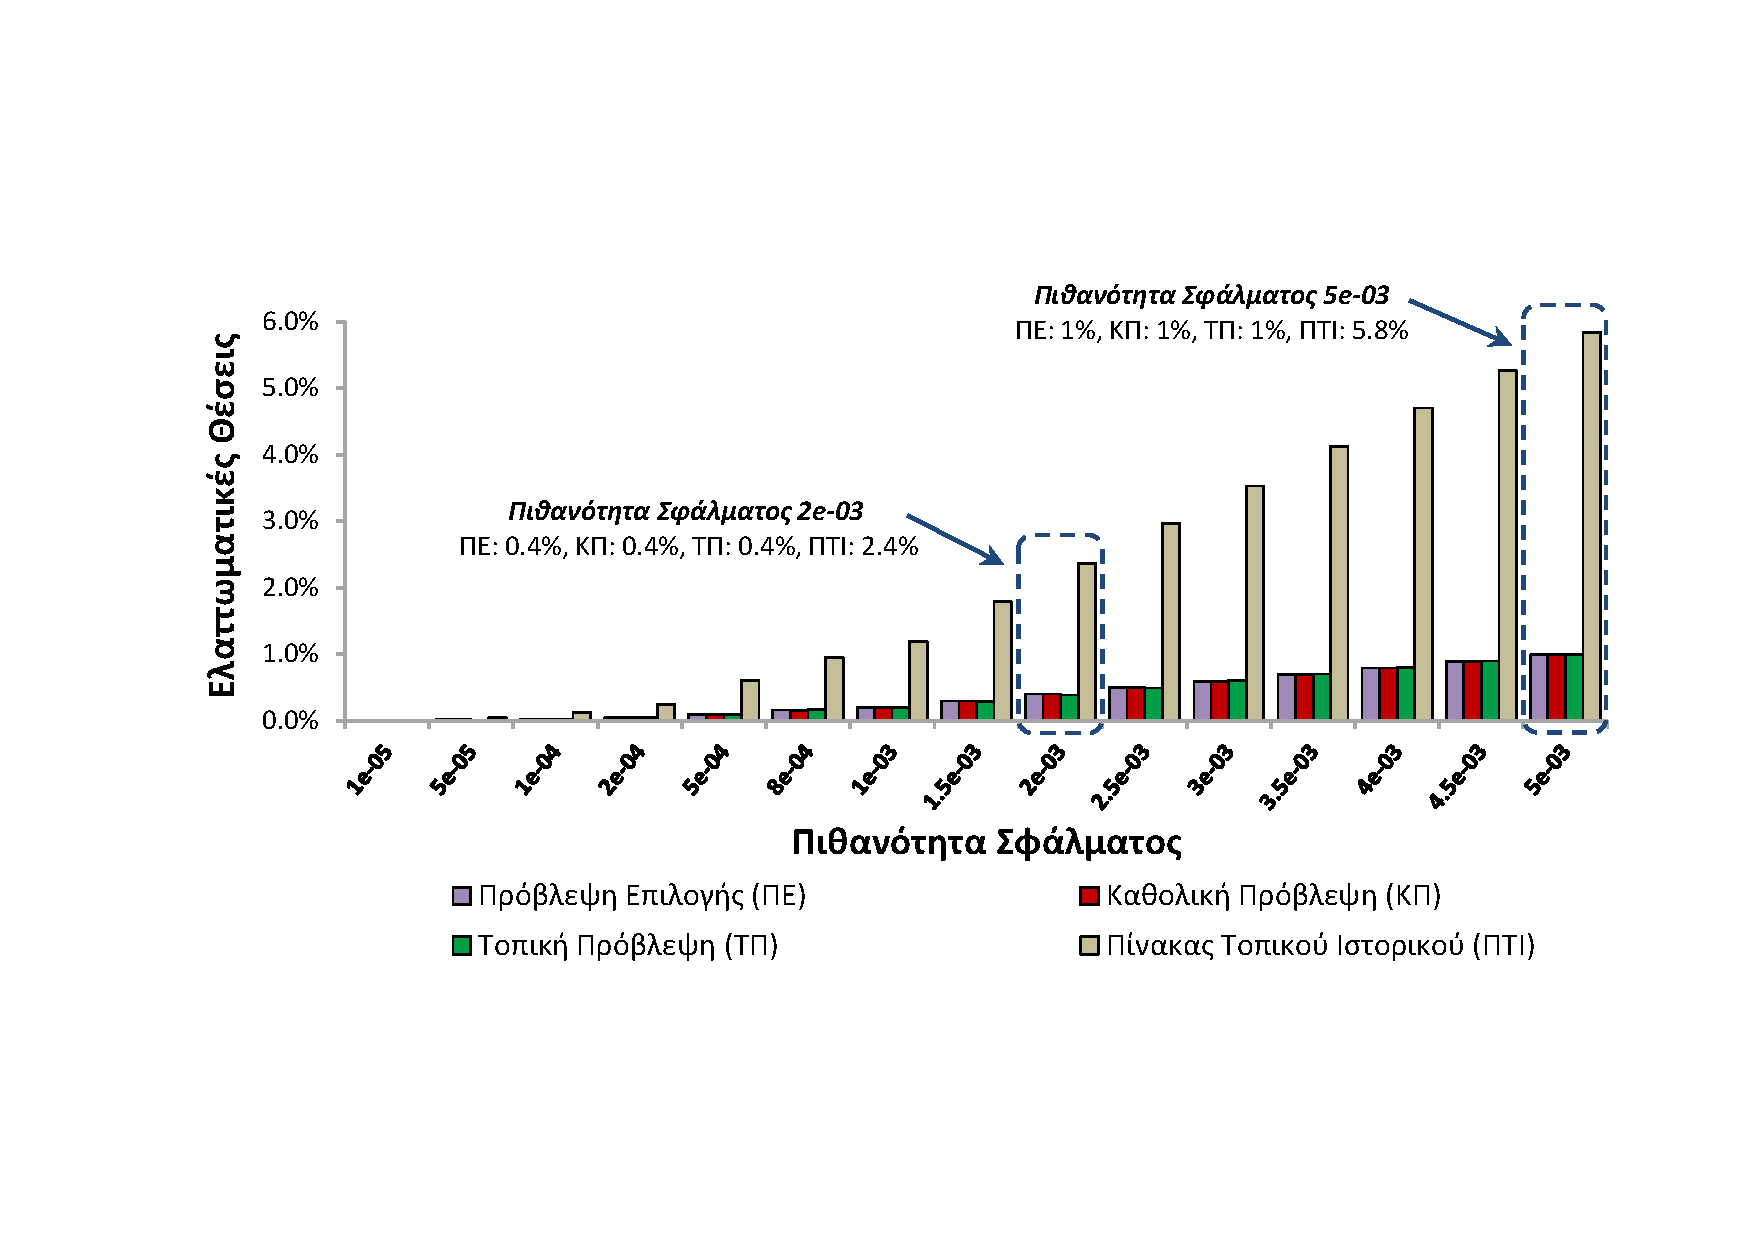
\includegraphics[width=0.9\linewidth, trim=3.4cm 4.7cm 2.2cm 4.8cm, clip=true]{\resultsDIR/chap4_BPU_faulty_entries.pdf}}
    \caption{Σφάλματα στον Πίνακα Πρόβλεψης Διακλάδωσης}
    \label{fig:chap4_bpu_fmaps}
\end{figure}

Όπως φαίνεται και από το γράφημα του Σχήματος \ref{fig:chap4_bpu_fmaps}, εξαιτίας του μικρού μεγέθους των στοιχείων μνήμης το ποσοστό ελαττωματικών θέσεων σε αυτές είναι σχετικά μικρό, ακόμη και σε μεγάλες πιθανότητες σφάλματος. Συγκεκριμένα, το πλήθος κυψελίδων κάθε στοιχείου μνήμης του Πίνακα Πρόβλεψης Διακλάδωσης είναι:

\begin{description} [itemsep=0.5pt]
    \item[Πρόβλεψη Επιλογής(ΠΕ):] 16384 θέσεις $\times$ 2 δ.ψ./θέση = 32768 κυψελίδες
    \item[Καθολική Πρόβλεψη(ΚΠ):] 16384 θέσεις $\times$ 2 δ.ψ./θέση = 32768 κυψελίδες
    \item[Τοπική Πρόβλεψη(ΚΠ):] 4096 θέσεις $\times$ 3 δ.ψ./θέση = 12288 κυψελίδες
    \item[Πίνακας Τοπικού Ιστορικού(ΠΤΙ):] 4096 θέσεις $\times$ 12 δ.ψ./θέση = 49152 κυψελίδες
    \item[Καταχωρητής Καθολικού Ιστορικού(ΚΚΙ):] 12 κυψελίδες
\end{description}

Με βάση τα ποσοστά του Σχήματος \ref{fig:chap4_bpu_fmaps} στη μέγιστη πιθανότητα σφάλματος $\expnum{5}$ στις διατάξεις πρόβλεψης το 1\% των θέσεων περιέχει τουλάχιστον ένα ελαττωματικό δυαδικό ψηφίο, ενώ στον Πίνακα Τοπικού Ιστορικού το ποσοστό αυτό ανέρχεται σε 5.8\%. Συνεπώς, αναμένεται πως οι επιπτώσεις της μείωσης της τάσης λειτουργίας θα είναι ελάχιστες στην επιτυχία του πρώτου επιπέδου πρόβλεψης. Η μείωση της απόδοσης εξαιτίας της ύπαρξης σφαλμάτων στον Πίνακα Πρόβλεψης Διακλάδωσης παρουσιάζεται στο Σχήμα \ref{fig:chap4_bpu_ipc}, όπου κατά μέσο όρο είναι μικρότερη από 1\%.

\begin{figure}[t]
    \centering
    \fbox{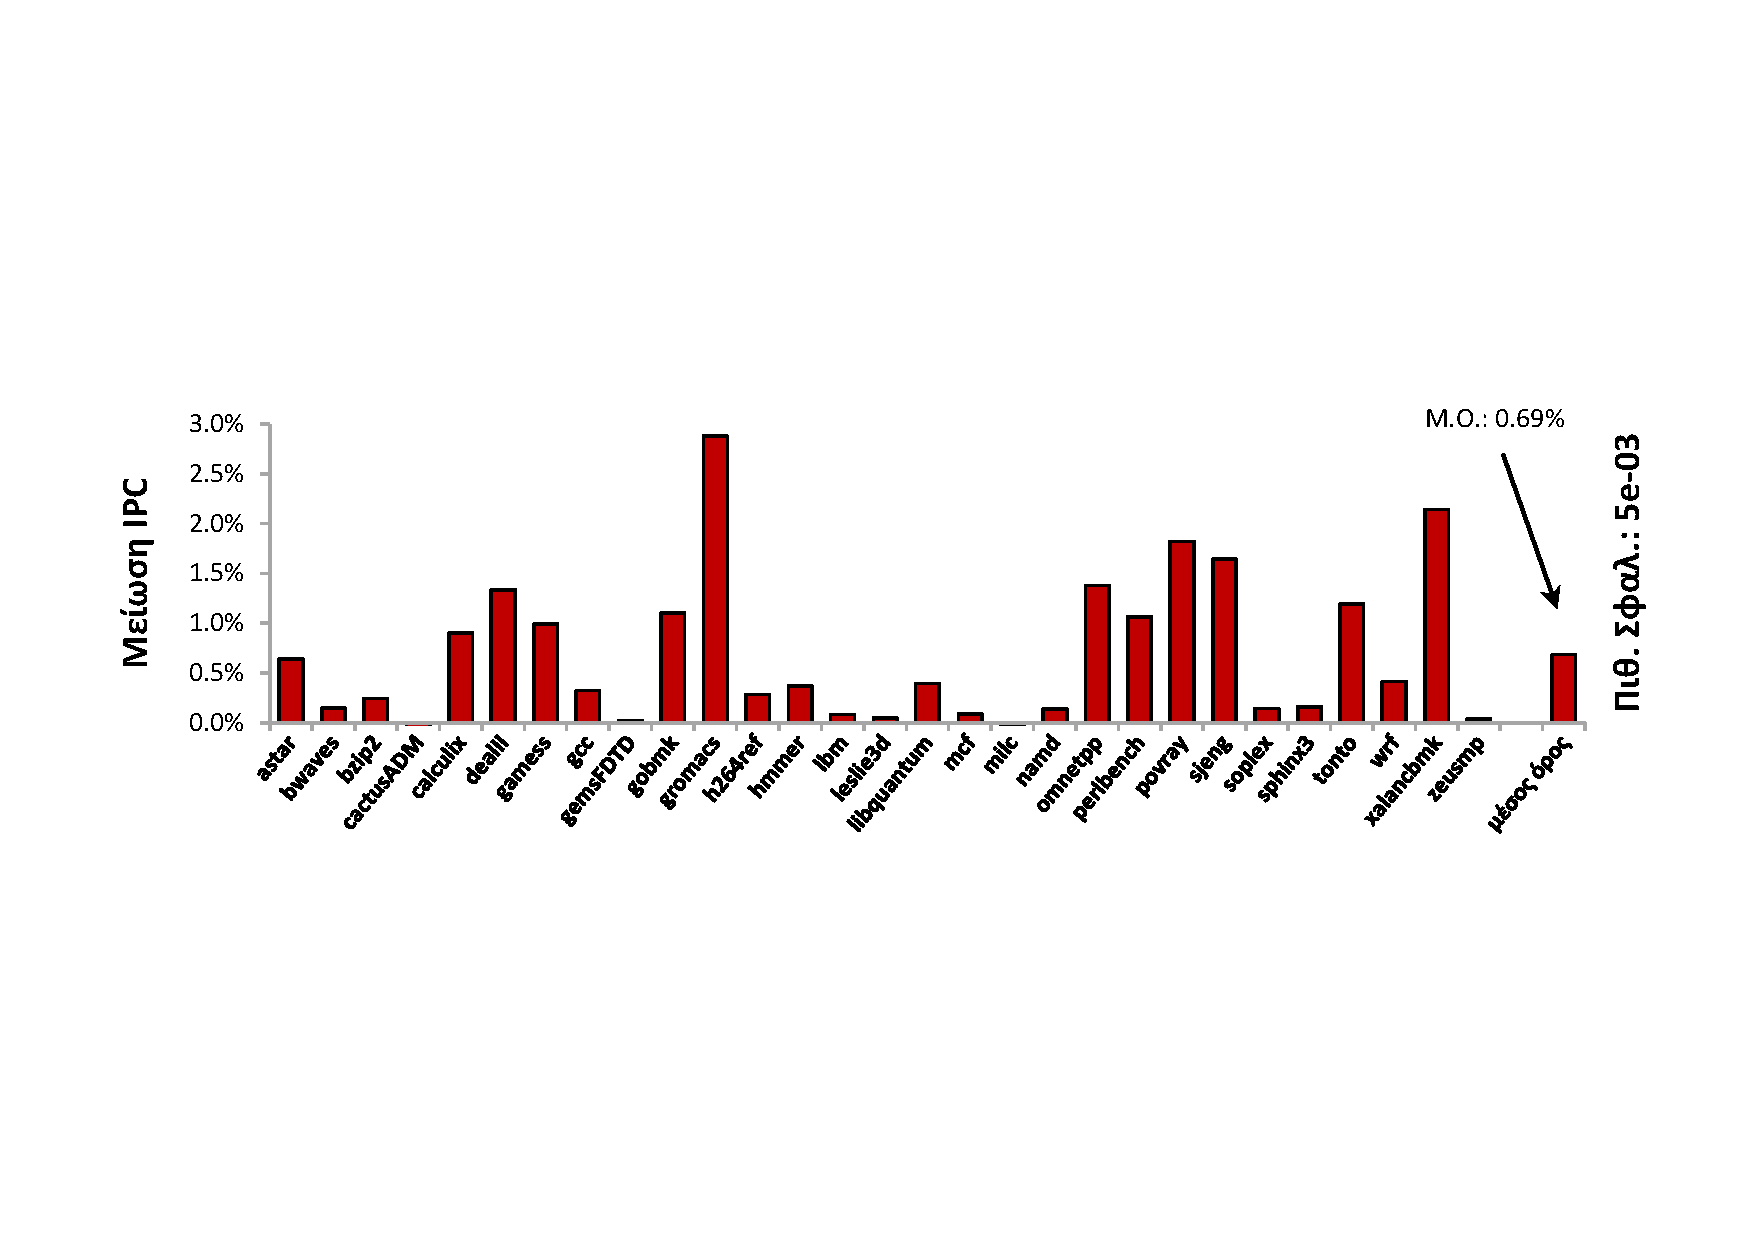
\includegraphics[width=\linewidth, trim=2cm 6.8cm 1.8cm 6.8cm, clip=true]{\resultsDIR/chap4_BPU_faulty_ipc.pdf}}
    \caption{Μείωση του ρυθμού ολοκλήρωσης εντολών εξαιτίας των σφαλμάτων στον Πίνακα Πρόβλεψης Διακλάδωσης, σε σχέση με την περίπτωση εφαρμογής της ονομαστικής τάσης στην ίδια συχνότητα λειτουργίας}
    \label{fig:chap4_bpu_ipc}
\end{figure}

\begin{figure}[!b]
    \centering
    \fbox{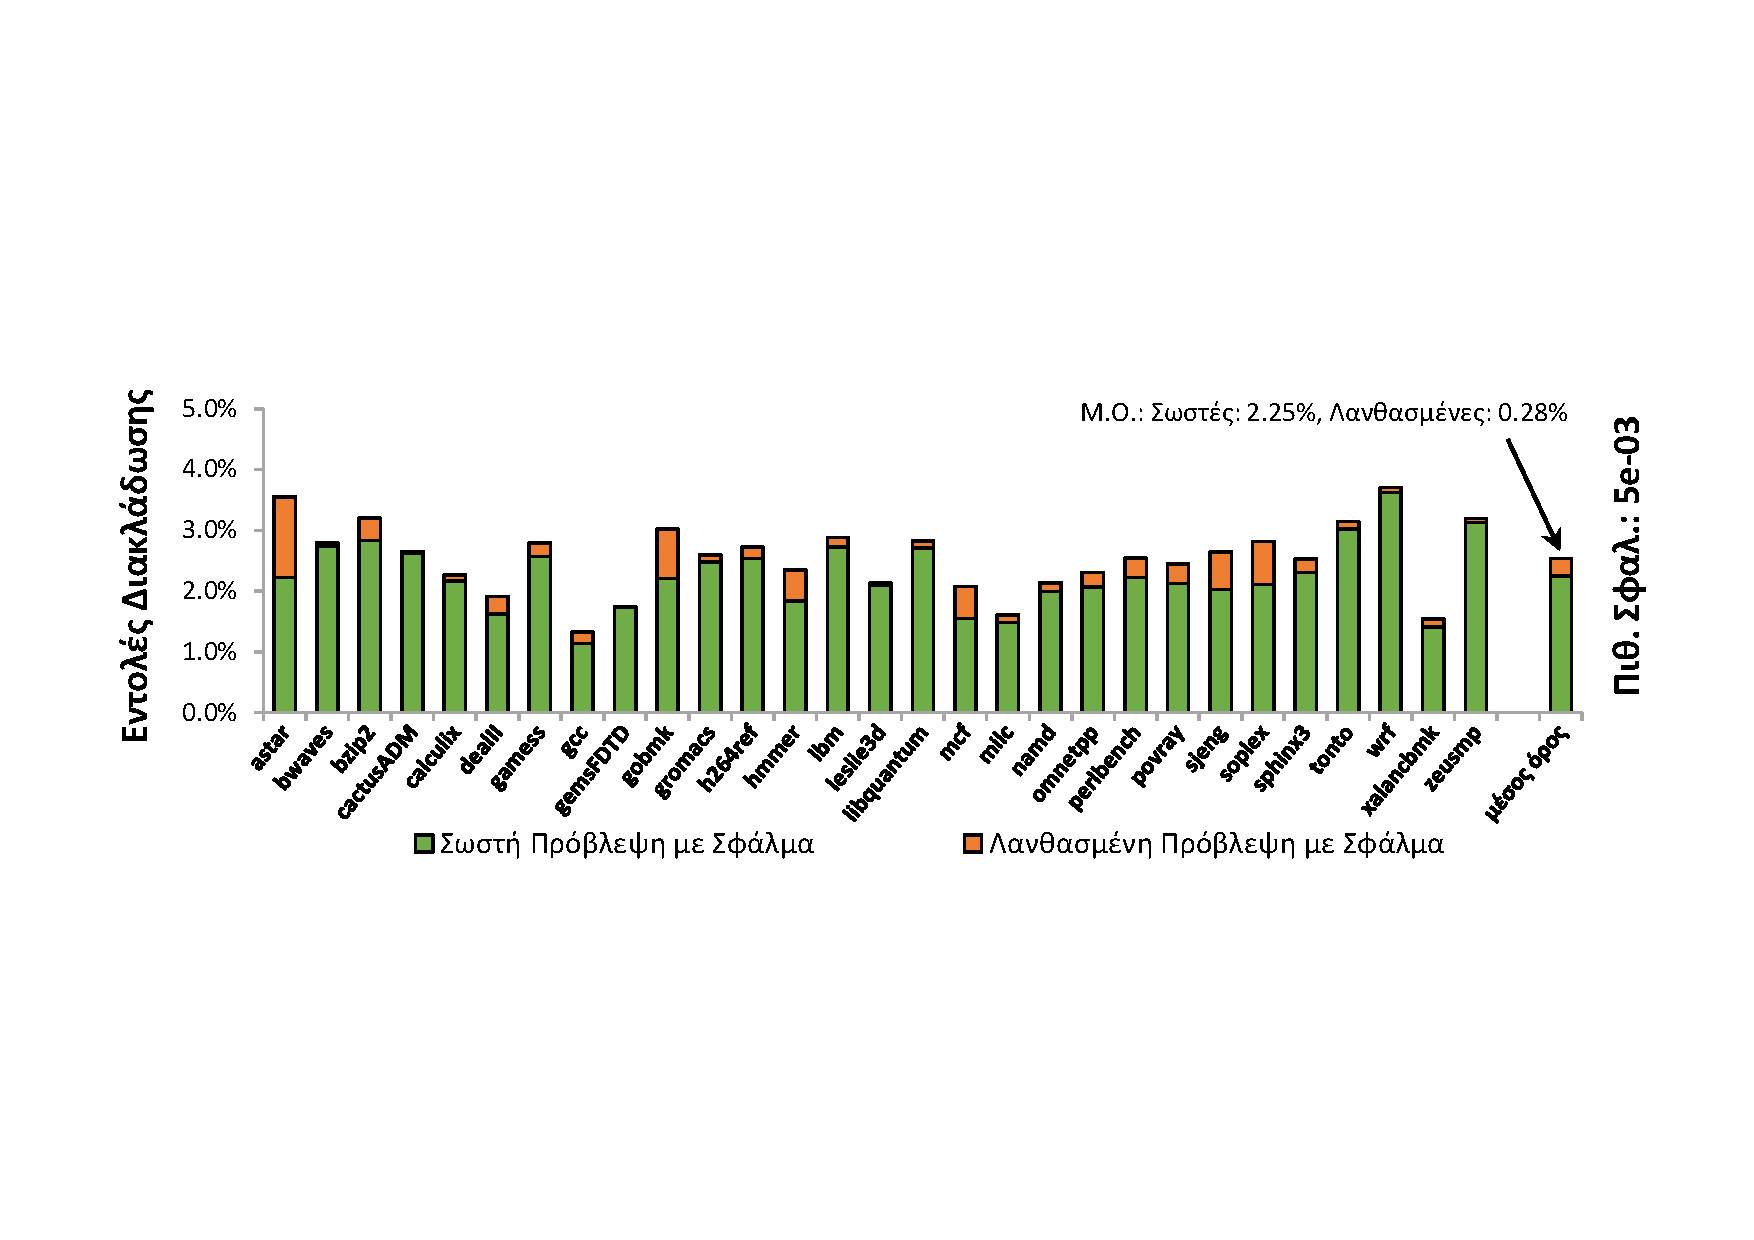
\includegraphics[width=\linewidth, trim=2cm 6.5cm 1.8cm 6.5cm, clip=true]{\resultsDIR/chap4_BPU_faulty_predictions.pdf}}
    \caption{Ποσοστό εκτελούμενων εντολών διακλάδωσης των οποίων η πρόβλεψη περιέχει κάποιο σφάλμα}
    \label{fig:chap4_bpu_branches}
\end{figure}

Για την περαιτέρω μελέτη των επιπτώσεων των σφαλμάτων αυτών, παρουσιάζεται το ποσοστό εντολών διακλάδωσης που εκτελέστηκαν και στις οποίες η εξαγωγή τελικής πρόβλεψης επηρεάστηκε από ελαττωματική θέση μνήμης. Μία τέτοια πρόβλεψη θα περιγράφεται ως πρόβλεψη με σφάλμα. Για παράδειγμα, έστω ότι η θέση που διαβάζεται από την Καθολική Πρόβλεψη περιέχει σφάλμα και η Πρόβλεψη Επιλογής διαλέξει την Καθολική Πρόβλεψη ως πιο έγκυρη, τότε η πρόβλεψη που θα εξαχθεί θα περιέχει σφάλμα. Μία πρόβλεψη με σφάλμα δεν συνεπάγεται πως είναι και λανθασμένη καθώς το σφάλμα μπορεί να προκαλέσει την εξαγωγή σωστής πρόβλεψης, όπως φαίνεται και στο γράφημα του Σχήματος \ref{fig:chap4_bpu_branches}, όπου το άθροισμα των ποσοστών πράσινων και πορτοκαλί αποχρώσεων ισοδυναμεί με το ποσοστό εντολών διακλάδωσης που εκτελέστηκαν και στην πρόβλεψή τους συμμετείχε στοιχείο με σφάλμα (προβλέψεις με σφάλμα), από το σύνολο των εντολών διακλάδωσης που εκτελέστηκαν.
\par
Από τις συνολικές εντολές διακλάδωσης που εκτελέστηκαν, σε μόλις 2.53\% αυτών θα έχουν συμμετάσχει ελαττωματικές κυψελίδες στην εξαγωγή πρόβλεψης. Επίσης, από το ποσοστό αυτό, μόνο στο 0.28\% αποδείχθηκε πως η πρόβλεψη με σφάλμα ήταν ταυτόχρονα και λανθασμένη. Παράδειγμα περίπτωσης όπου ένα σφάλμα μπορεί να μην προκαλέσει καμία μείωση στην ευστοχία αποτελεί η περίπτωση όπου η Πρόβλεψη Επιλογής περιέχει σφάλμα και εξαιτίας αυτού επιλέγεται το αποτέλεσμα της Τοπικής αντί της Καθολικής Πρόβλεψης. Εάν η Τοπική Πρόβλεψη αποδειχθεί σωστή τότε η επίπτωση αυτού του σφάλματος θα είναι μηδενική.
\par
Από τη μελέτη της παρούσας υποενότητας κατέστη σαφές πως η ανάπτυξη κατάλληλης τεχνικής ανοχής σφαλμάτων του Πίνακα Πρόβλεψης Διακλάδωσης δεν είναι απαραίτητη. Για το λόγο αυτό η παρούσα μελέτη επικεντρώνεται στα σφάλματα που εμφανίζονται στον Πίνακα Πρόβλεψης Διακλάδωσης, της οποίας το μέγεθός είναι αρκετά μεγαλύτερο και επομένως αναμένεται να εμφανίσει σημαντικό πλήθος ελαττωματικών στοιχείων.

%----------------------------------------------------------%

\subsection{Σφάλματα στον Πίνακα Πρόβλεψης Προορισμού Διακλάδωσης}
\label{chap4_BranchTargetBufferFaults}

Όπως είναι αναμενόμενο, η μεγάλη μείωση της τάσης λειτουργίας θα επηρεάσει και τη λειτουργία του Πίνακα Πρόβλεψης Προορισμού Διακλάδωσης. Η εμφάνιση σφαλμάτων στον πίνακα θα έχει ως συνέπεια την υποβάθμιση της ακρίβειας πρόβλεψης διευθύνσεων και επομένως της απόδοσης. Για να εξασφαλιστεί πως δεν θα ληφθεί λανθασμένη διεύθυνση εξαιτίας ενός σφάλματος στον Πίνακα Πρόβλεψης Προορισμού Διακλάδωσης, κάτι που μπορεί να επιφέρει σημαντική αύξηση του χρόνου εκτέλεσης του προγράμματος, τα πλαίσια που περιέχουν τουλάχιστον μία ελαττωματική κυψελίδα απενεργοποιούνται χρησιμοποιώντας την τεχνική απενεργοποίησης πλαισίου, η οποία εφαρμόζεται συχνά στην Κρυφής Μνήμη πρώτου επιπέδου όπως αναφέρθηκε στην Ενότητα \ref{chap3_FaultTaulerance}. Για την υλοποίηση αυτής της τεχνικής αρκεί η προσθήκη ενός δυαδικού ψηφίου ανά θέση μνήμης, το αποκαλούμενο ως $``$Ψηφίο Σφάλματος$"$, το οποίο δηλώνει εάν ανιχνεύτηκε ελαττωματική κυψελίδα στην αντίστοιχη θέση κατά τη διαδικασία του ελέγχου.
\par
Στην παρούσα υποενότητα μελετάται η επιρροή που θα έχει η μείωση του έγκυρου χώρου αποθήκευσης του Πίνακα Πρόβλεψης Προορισμού Διακλάδωσης (ΠΠΠΔ), το ποσοστό του οποίου παρουσιάζεται στο Σχήμα \ref{fig:chap4_btb_fmaps}.

\begin{figure}[!t]
    \centering
    \fbox{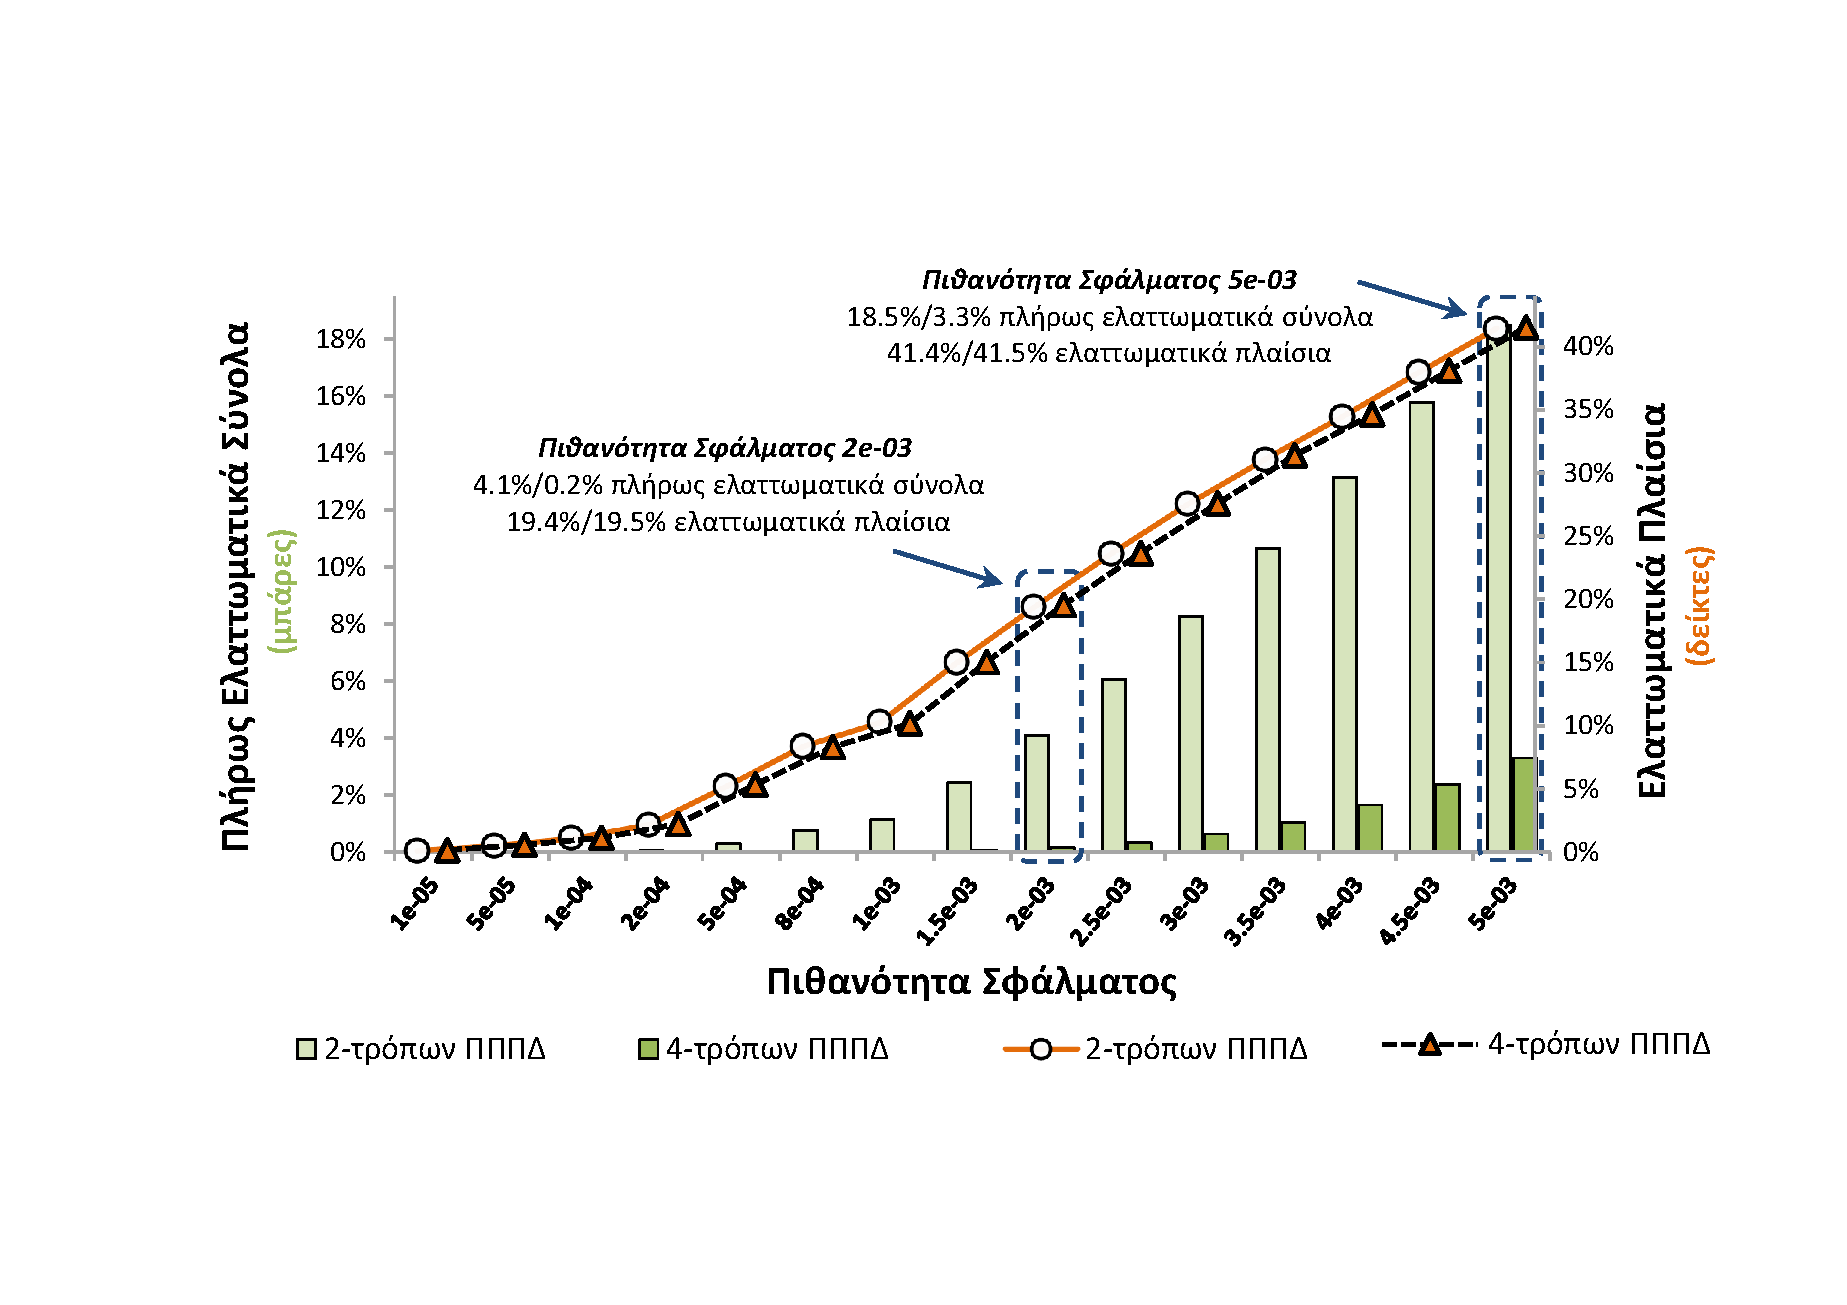
\includegraphics[width=0.9\linewidth, trim=3.5cm 4cm 2cm 4.3cm, clip=true]{\resultsDIR/chap4_BTB_faulty_entries_and_sets.pdf}}
    \caption{Σφάλματα στον Πίνακα Πρόβλεψης Προορισμού Διακλάδωσης (ΠΠΠΔ)}
    \label{fig:chap4_btb_fmaps}
\end{figure}

Το γράφημα του Σχήματος \ref{fig:chap4_btb_fmaps} αποτελείται από δύο κατηγορίες δεδομένων. Οι μπάρες πράσινων αποχρώσεων παριστάνουν το ποσοστό των πλήρως ελαττωματικών συνόλων, δηλαδή τα σύνολα που όλα τα πλαίσια περιέχουν τουλάχιστον μία ελαττωματική κυψελίδα (κάθετος άξονας αριστερά). Το χαρακτηριστικό αυτών των θέσεων είναι η αδυναμία αποθήκευσης πληροφορίας για ένα πλήθος εντολών διακλάδωσης. Το δεύτερο δεδομένο, το οποίο αναπαρίσταται στο γράφημα με τη μορφή δεικτών στις νοητές καμπύλες πορτοκαλί και μαύρων αποχρώσεων, εκφράζουν το αντίστοιχο ποσοστό των ελαττωματικών πλαισίων για κάθε πιθανότητα σφάλματος (κάθετος άξονας δεξιά). Τα σχετικά μικρού μεγέθους πλαίσια, τα οποία αποτελούνται από τα πεδία ετικέτας, διεύθυνσης προορισμού και ορισμένες ακόμα πληροφορίες, συνεπάγονται τη σχετικά μικρή πιθανότητα μίας θέσης να είναι ελαττωματική, συγκριτικά με μία θέση Κρυφής Μνήμης (λιγότερα δυαδικά ψηφία ανά πλαίσιο συνεπάγεται και μικρότερη πιθανότητα να είναι ελαττωματικό). Το γράφημα του Σχήματος \ref{fig:chap4_btb_fmaps} εκφράζει το μέσο όρο 100 χαρτών σφαλμάτων για κάθε πιθανότητα σφάλματος.
\par
Τα δεδομένα κάθε χάρτη σφαλμάτων εισάγονται στα αντίστοιχα δυαδικά ψηφία σφάλματος του πίνακα, ώστε να πραγματοποιηθεί εξομοίωση με απενεργοποίηση των πλαισίων που έχουν ελαττωματικές κυψελίδες. Για την διερεύνηση των επιπτώσεων τους στην απόδοση του υπερβαθμωτού επεξεργαστή, εξετάζεται η λειτουργία σε δύο διαφορετικές τάσεις χαμηλού δυναμικού οι οποίες αντιστοιχούν σε δύο πιθανότητες σφάλματος (πιθανότητα-1: $\expnum{2}$ και πιθανότητα-2: $\expnum{5}$) για κάθε οργάνωση. Η αναλυτική αντιστοίχηση μελετώμενων τάσεων και πιθανοτήτων παρουσιάζεται στο Κεφάλαιο \ref{chap6}. Το σύνολο των εξομοιώσεων που πραγματοποιήθηκαν για τη λειτουργία χαμηλού δυναμικού αναγράφονται στον Πίνακα \ref{tab:chap4_LowPowerSimulations}.

\begin{table}[!b]
    \centering
    \begin{tabularx}{\textwidth}{!{\vrule width 4\arrayrulewidth} >{\centering\arraybackslash}X | c !{\vrule width 4\arrayrulewidth}}
        \Xhline{4\arrayrulewidth}
        \textbf{Οργάνωση ΠΠΠΔ}                 & \textbf{Πιθανότητα Σφάλματος (Συχνότητα)} \\
        \Xhline{4\arrayrulewidth}
        \multirow{2}{*}{2048-πλαίσια/2-τρόπων} & {$\expnum{2}\ (1.1GHz)$} \\ \cline{2-2}
        & {$\expnum{5}\ (0.5GHz)$} \\
        \hline
        \multirow{2}{*}{2048-πλαίσια/4-τρόπων} & {$\expnum{2}\ (1.1GHz)$} \\ \cline{2-2}
        & {$\expnum{5}\ (0.5GHz)$} \\
        \hline
        \hline
        \textbf{Σύνολο Εξομοιώσεων}            & {4 $\times$ 29 μετροπρογράμματα $\times$ 100 χάρτες σφ. = \textbf{11600}} \\
        \Xhline{4\arrayrulewidth}
    \end{tabularx}
    \caption{Εκτελούμενες εξομοιώσεις σε λειτουργία χαμηλής κατανάλωσης}
    \label{tab:chap4_LowPowerSimulations}
\end{table}

Οι εξομοιώσεις που πραγματοποιήθηκαν για την εφαρμογή της ονομαστικής τάσης λειτουργίας (κανονική λειτουργία), όπου όλα τα πλαίσια είναι ενεργοποιημένα, αναγράφονται στον Πίνακα \ref{tab:chap4_NominalSimulations}.

\begin{table}[!t]
    \centering
    \begin{tabularx}{\textwidth}{!{\vrule width 4\arrayrulewidth} >{\centering\arraybackslash}X | >{\centering\arraybackslash}X !{\vrule width 4\arrayrulewidth}}
        \Xhline{4\arrayrulewidth}
        \textbf{Οργάνωση ΠΠΠΔ}                 & \textbf{Συχνότητα Λειτουργίας} \\
        \Xhline{4\arrayrulewidth}
        \multirow{2}{*}{2048-πλαίσια/2-τρόπων} & {$1.1 GHz$} \\ \cline{2-2}
        & {$0.5 GHz$} \\
        \hline
        \multirow{2}{*}{2048-πλαίσια/4-τρόπων} & {$1.1 GHz$} \\ \cline{2-2}
        & {$0.5 GHz$} \\
        \hline
        \hline
        \textbf{Σύνολο Εξομοιώσεων}            & {4 $\times$ 29 μετροπρογράμματα = \textbf{116}} \\
        \Xhline{4\arrayrulewidth}
    \end{tabularx}
    \caption{Εκτελούμενες εξομοιώσεις σε κανονική λειτουργία}
    \label{tab:chap4_NominalSimulations}
\end{table}

Ο μέσος όρος των 100 εξομοιώσεων, για κάθε παραμετροποίηση του Πίνακα Πρόβλεψης Προορισμού Διακλάδωσης και εκτελούμενο μετροπρόγραμμα, παρουσιάζεται στις γραφικές παραστάσεις του Σχήματος \ref{fig:chap4_faulty_ipc}. Τα αποτελέσματα αναφέρονται στη μείωση που δέχεται ο ρυθμός ολοκλήρωσης εντολών (\ipc) εξαιτίας της εμφάνισης σφαλμάτων στον Πίνακα Πρόβλεψης Προορισμού Διακλάδωσης όταν η τάση λειτουργίας μειώνεται, συγκριτικά με την εκτέλεση υπό κανονική λειτουργία στην ίδια συχνότητα. 

\begin{figure}[!b]
    \centering
    \begin{subfigure}[t]{\textwidth}
        \centering
        \fbox{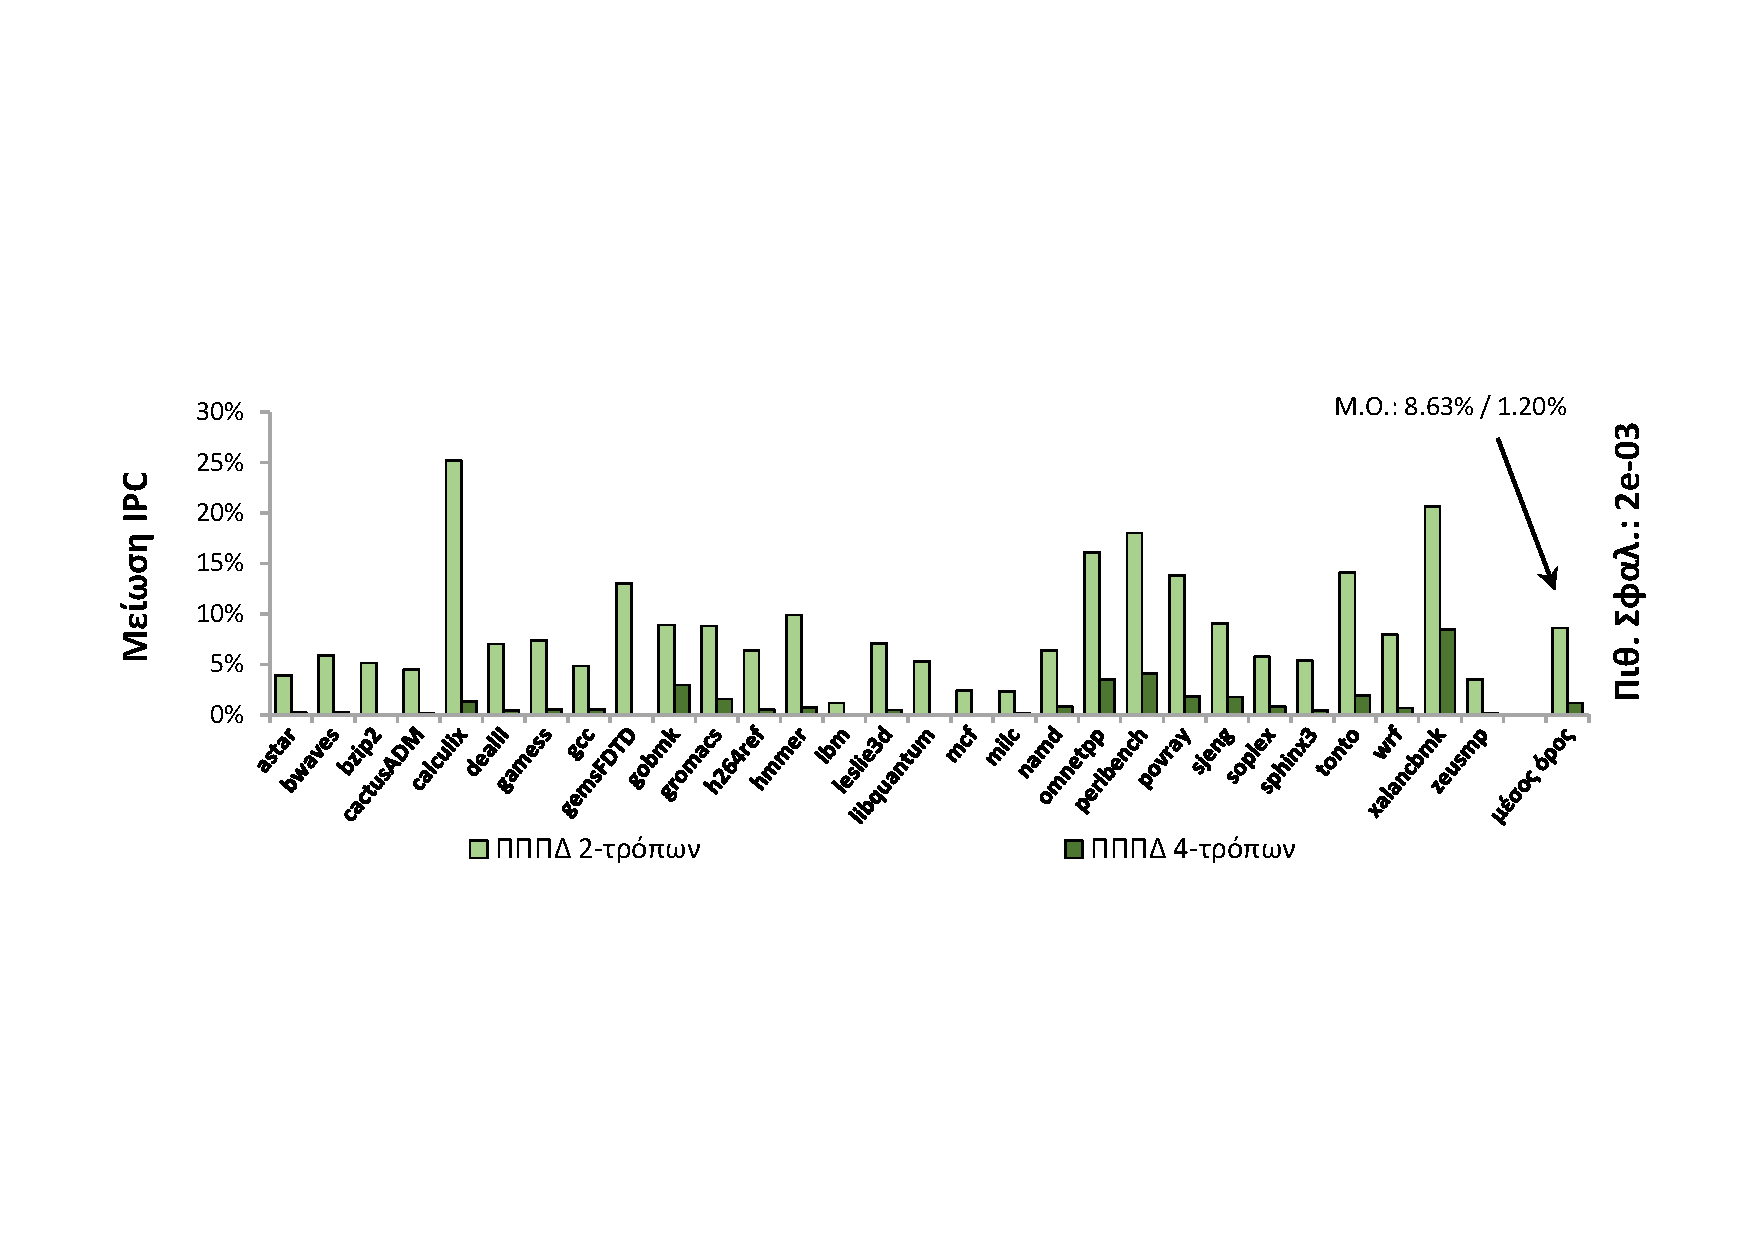
\includegraphics[width=\linewidth, trim=1.9cm 6.4cm 1.8cm 6.6cm, clip=true]{\resultsDIR/chap4_BTB_faulty_ipc_pfail1.pdf}}
        \caption{Πιθανότητα Σφάλματος 1}
        \label{fig:chap4_faulty_pail1_ipc}
    \end{subfigure}
    
    \begin{subfigure}[t]{\textwidth}
        \centering
        \fbox{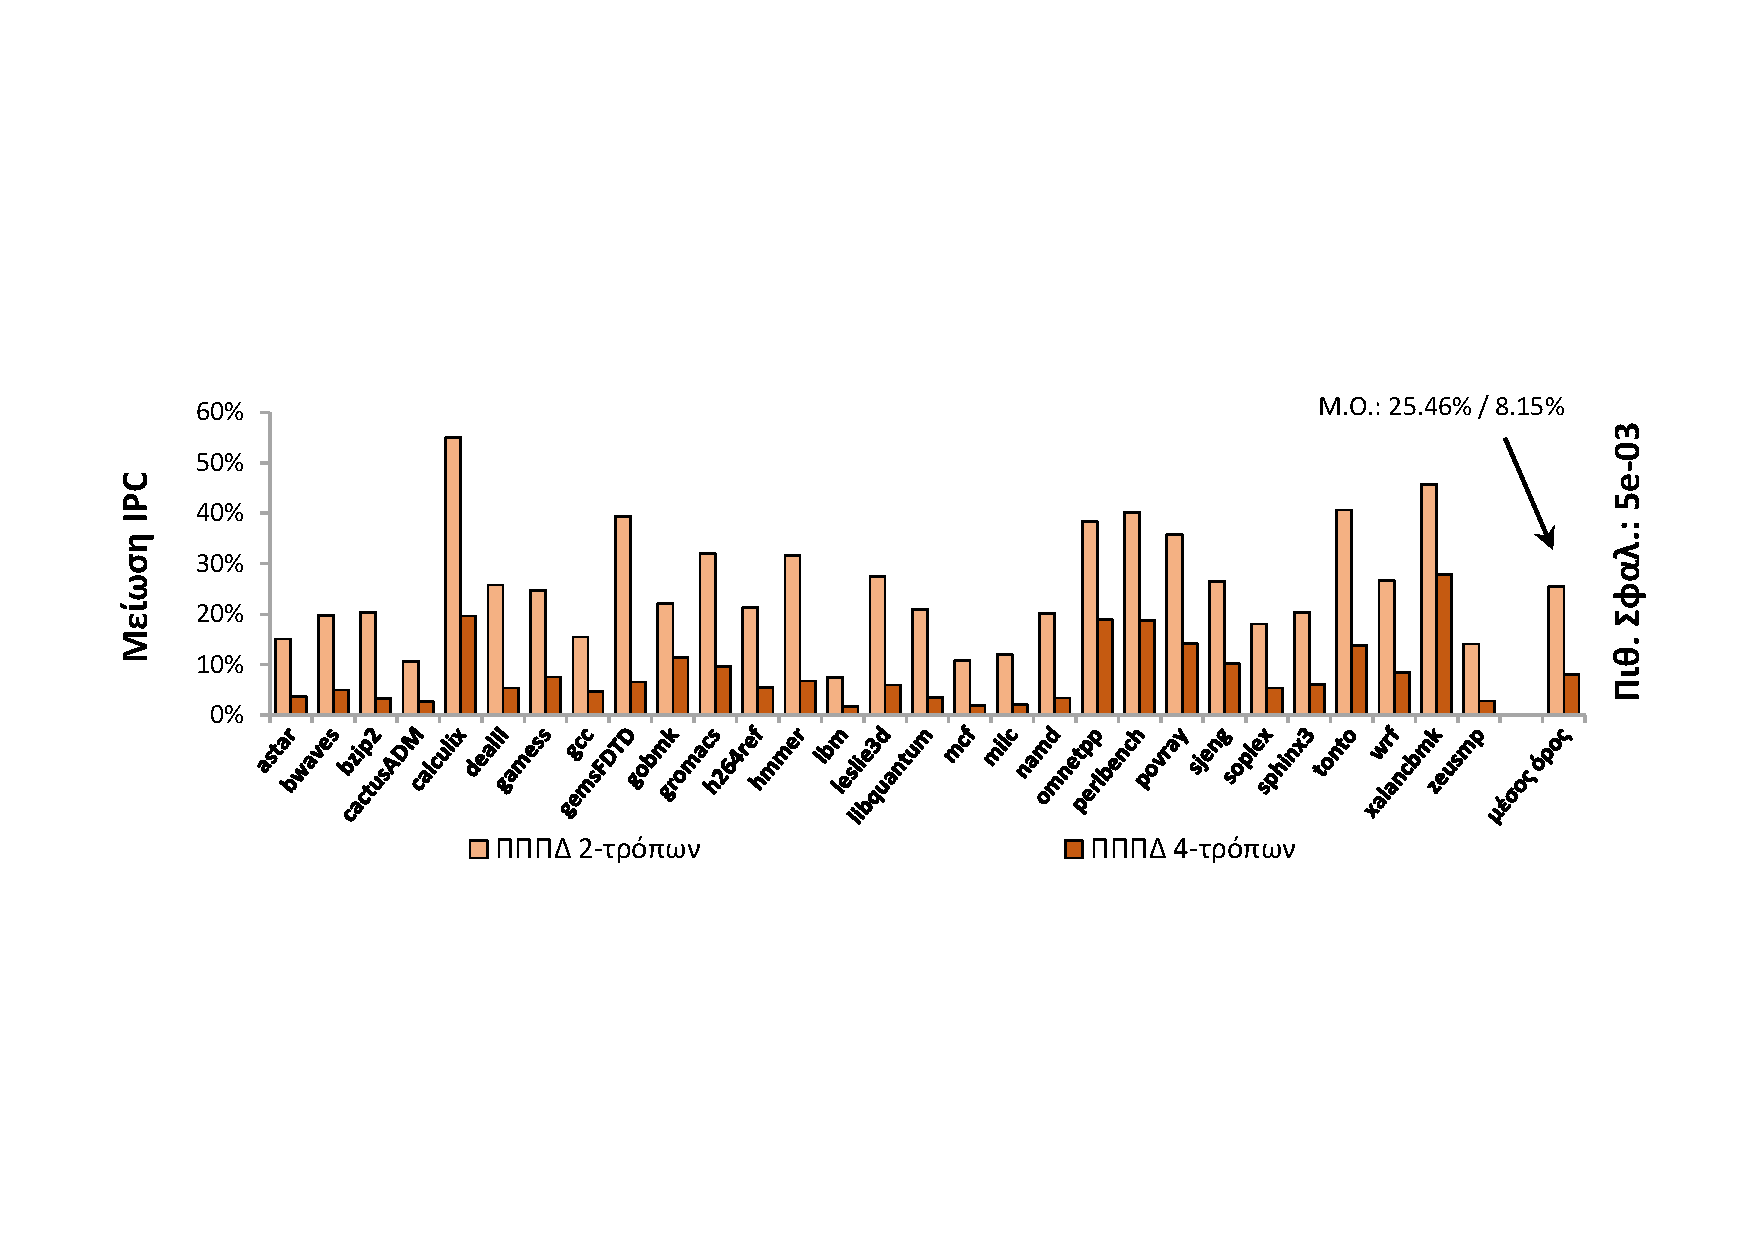
\includegraphics[width=\linewidth, trim=1.9cm 6.4cm 1.8cm 6.6cm, clip=true]{\resultsDIR/chap4_BTB_faulty_ipc_pfail2.pdf}}
        \caption{Πιθανότητα Σφάλματος 2}
        \label{fig:chap4_faulty_pail2_ipc}
    \end{subfigure}
    \caption{Μείωση του ρυθμού ολοκλήρωσης εντολών εξαιτίας της ύπαρξης σφαλμάτων στον Πίνακα Πρόβλεψης Προορισμού Διακλάδωσης, σε σχέση με την περίπτωση εφαρμογής της ονομαστικής τάσης στην ίδια συχνότητα λειτουργίας}
    \label{fig:chap4_faulty_ipc}
\end{figure}

Όπως αναγράφονται και στα αντίστοιχα γραφήματα, το μέγεθος της μείωσης της απόδοσης διαφέρει μεταξύ των πιθανοτήτων και οργανώσεων. Σε μνήμες οργάνωσης 2-τρόπων συνόλου συσχέτισης, στην μελετώμενη πιθανότητα σφάλματος 1 ($\expnum{2}$) η μείωση της απόδοσης φτάνει το 8.63\% κατά μέσο όρο, ενώ στην πιθανότητα σφάλματος 2 ($\expnum{5}$) η μείωση αυτή ξεπερνά το 25\%. Σε μνήμες οργάνωσης 4-τρόπων οι αντίστοιχες μειώσεις κατά μέσο όρο είναι 1.2\% στην πιθανότητα σφάλματος 1, και λίγο πάνω από 8\% στην πιθανότητα σφάλματος 2. Παρόλα αυτά, όπως φαίνεται και στα γραφήματα, υπάρχουν περιπτώσεις μετροπρογραμμάτων όπου η επίπτωση των σφαλμάτων είναι πολύ μεγαλύτερη του μέσου όρου, όπως για παράδειγμα το μετροπρόγραμμα \en{xalancbmk}.

%----------------------------------------------------------%

\section{Μεταβολή της Απόδοσης}
\label{chap4_PerformanceVariation}

Η παρούσα ενότητα συμβάλει στην καλύτερη κατανόησης των περιπτώσεων όπου η μεταβολή της απόδοσης του Πίνακα Πρόβλεψης Προορισμού Διακλάδωσης επιφέρει μεταβολή στην απόδοση του υπερβαθμωτού επεξεργαστή. Η πρώτη υποενότητα επικεντρώνεται στην οργάνωση του Πίνακα Πρόβλεψης Προορισμού Διακλάδωσης (ΠΠΠΔ) και παρουσιάζει την αύξηση της απόδοσης καθώς το μέγεθος και το πλήθος των τρόπων συσχέτισης αυξάνεται, όταν το ολοκληρωμένο λειτουργεί στην ονομαστική τάση. Στη δεύτερη υποενότητα μελετάται πως ο βαθμός παραλληλίας της Κεντρικής Μονάδας Επεξεργασίας (ΚΜΕ) μεταβάλει την επιρροή που έχουν τα σφάλματα του Πίνακα Πρόβλεψης Προορισμού Διακλάδωσης στην απόδοση του συστήματος. Τα αποτελέσματα φανερώνουν εάν και πότε είναι ωφέλιμο να αντιμετωπιστούν τα σφάλματα αυτά.

%----------------------------------------------------------%

\subsection{Οργάνωση ΠΠΠΔ}
\label{chap4_BTBConfigIPC}

\begin{figure}[!b]
    \centering
    \fbox{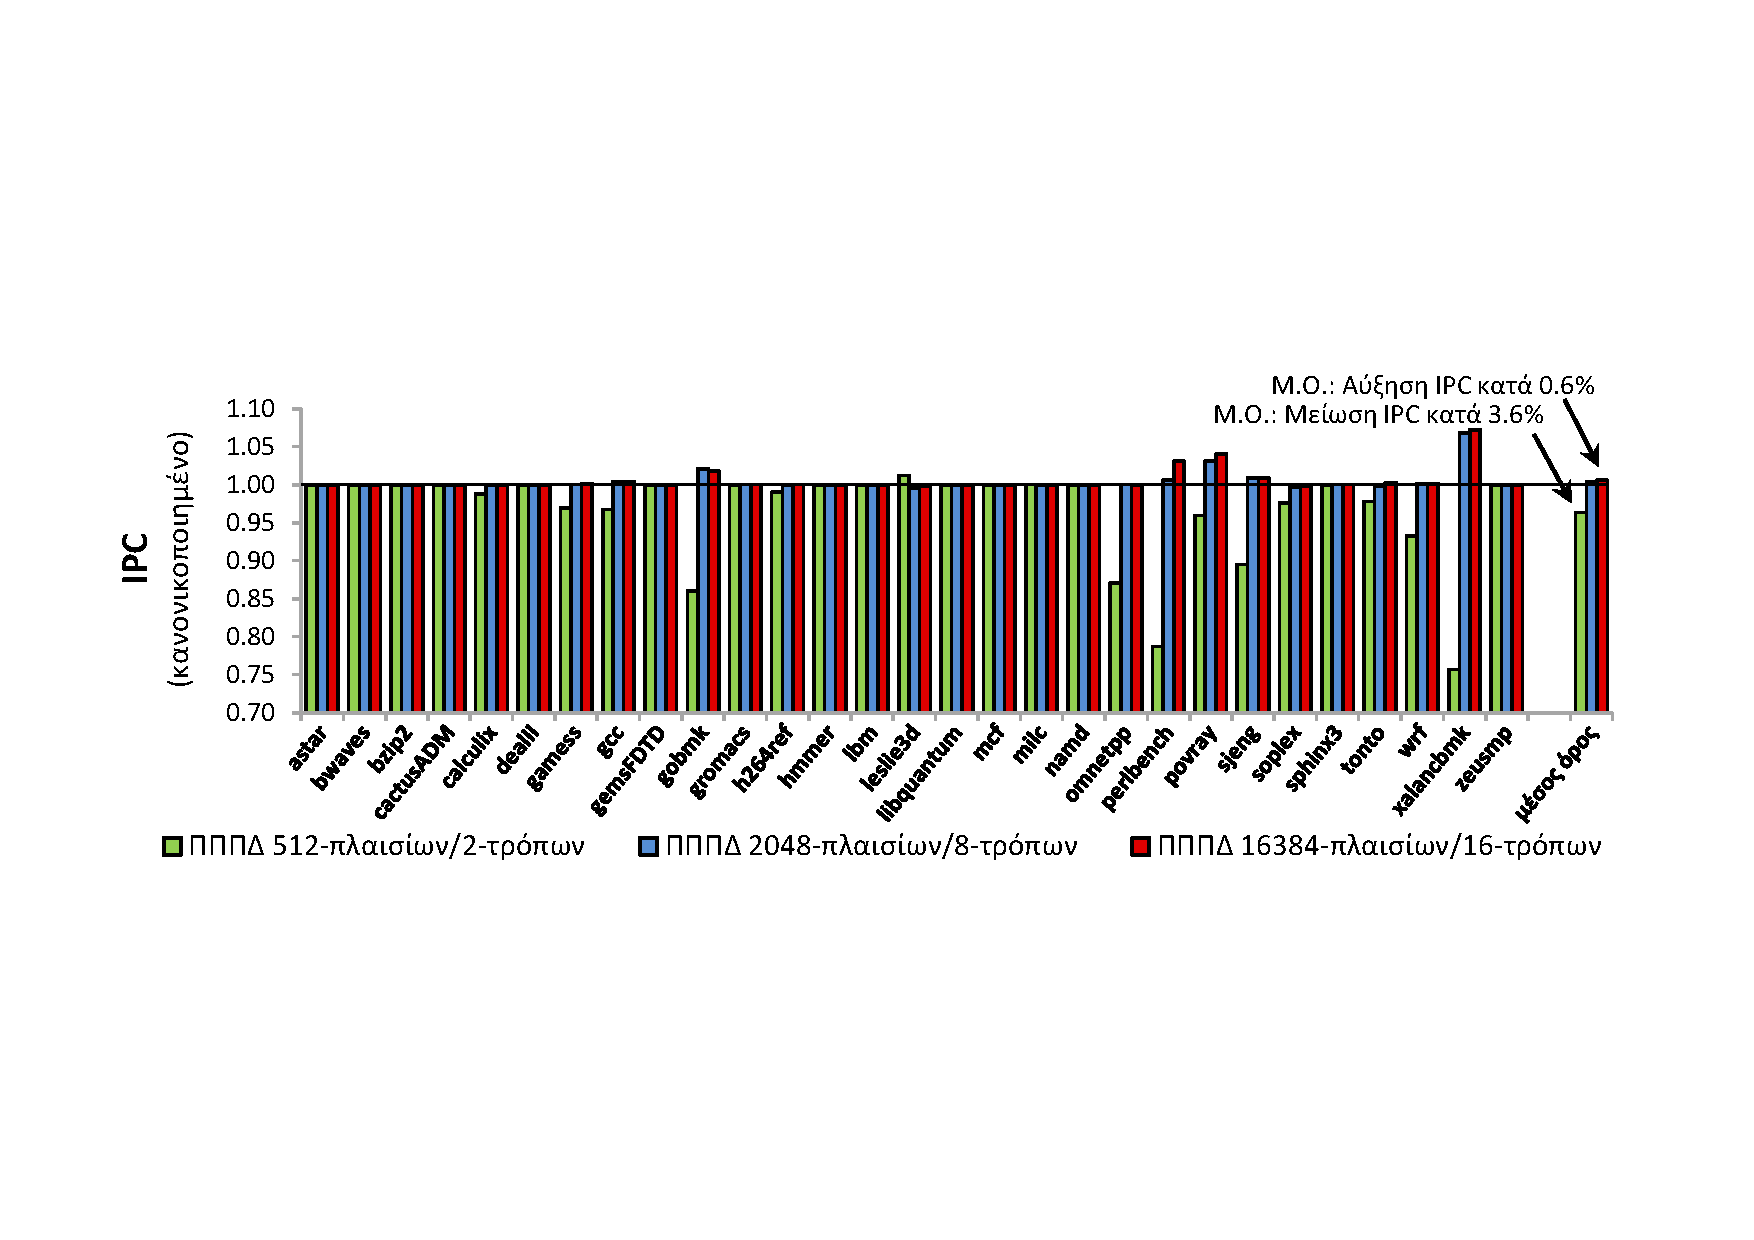
\includegraphics[width=\linewidth, trim=1.9cm 6.4cm 1.8cm 6.3cm, clip=true]{\resultsDIR/chap4_BTB_configs_ipc.pdf}}
    \caption{Ρυθμός ολοκλήρωσης εντολών για διαφορετικές παραμετροποιήσεις του Πίνακα Πρόβλεψης Προορισμού Διακλάδωσης (κανονικοποιημένος ως προς την περίπτωση 2048-πλαισίων/2-τρόπων)}
    \label{fig:chap4_btb_config_performance}
\end{figure}

Στο Σχήμα \ref{fig:chap4_btb_config_performance} παρουσιάζεται η μεταβολή του αριθμού εντολών που ολοκληρώνονται ανά κύκλο (\ipc), με τη μεταβολή του μεγέθους και της οργάνωσης του Πίνακα Πρόβλεψης Προορισμού Διακλάδωσης (ΠΠΠΔ). Τα αποτελέσματα αναφέρονται στην περίπτωση όπου εφαρμόζεται κανονική τάση λειτουργίας και είναι κανονικοποιημένα ως προς την περίπτωση που χρησιμοποιείται Πίνακας Πρόβλεψης Προορισμού Διακλάδωσης 2048 πλαισίων και 2-τρόπων συνόλου συσχέτισης.
\par
Όπως φανερώνεται από το γράφημα του Σχήματος \ref{fig:chap4_btb_config_performance}, η αύξηση του μεγέθους του Πίνακα Πρόβλεψης Προορισμού Διακλάδωσης επηρεάζει ελάχιστα την απόδοση από ένα σημείο κι έπειτα. Συγκεκριμένα, η χρήση πίνακα 512 αντί 2048 πλαισίων (μπάρες πράσινου χρώματος), θα έχει ως αποτέλεσμα τη μείωση του ρυθμού ολοκλήρωσης εντολών κατά 3.6\%, κατά μέσο όρο. Από την άλλη πλευρά, η χρήση ενός πίνακα των 16384 αντί 2048 πλαισίων (μπάρες κόκκινου χρώματος), προσφέρει κατά μέσο όρο λιγότερο από 1\% βελτίωση στο ρυθμού ολοκλήρωσης εντολών.
\par
Μελετώντας τη μεταβολή της απόδοσης με τη μεταβολή του πλήθους τρόπων συσχέτισης, γίνεται αντιληπτό πως η αύξηση του πλήθους πλαισίων ανά σύνολο δεν συνεισφέρει στη βελτίωση της απόδοσης (σχέση μεταξύ πίνακα 2048-πλαισίων/2-τρόπων και 2048-πλαισίων/8-τρόπων). Κατά μέσο όρο όταν χρησιμοποιείται ο πίνακας 2048-πλαισίων/8-τρόπων η βελτίωση είναι μικρότερη από 0.5\% (μπάρες γαλάζιου χρώματος). Ιδιαίτερη μεταβολή στην απόδοση παρουσιάζει το μετροπρόγραμμα \en{xalancbmk}, όπου όταν χρησιμοποιηθεί πίνακας του ίδιο μεγέθους (2048-πλαισίων) αλλά τετραπλάσιας συσχέτισης (8-τρόπων αντί για 2-τρόπων), παρουσιάζει βελτίωση μεγαλύτερη από 7\%. Αντίστοιχα, όταν το μέγεθος και το πλήθος των τρόπων συσχέτισης μειώνονται (από πίνακα 2048-πλαισίων/2-τρόπων σε πίνακα 512-πλαισίων/2-τρόπων), η μείωση της απόδοσης ξεπερνά το 24\%.
\par
Επομένως, για τη εκτέλεσης μίας μέσης περίπτωσης προγράμματος είναι προτιμότερο κατά το σχεδιασμό του υπερβαθμωτού επεξεργαστή να χρησιμοποιείται Πίνακας Πρόβλεψης Προορισμού Διακλάδωσης 2048-πλαισίων και μικρού σχετικά πλήθους πλαισίων ανά σύνολο, μειώνοντας έτσι την κατανάλωση σε σχέση με ένα πίνακα μεγαλύτερου μεγέθους και πλήθους πλαισίων ανά σύνολο.

%----------------------------------------------------------%

\subsection{Παραλληλία ΚΜΕ και Σφάλματα ΠΠΠΔ}
\label{chap4_CoreConfigIPC}

Στο Σχήμα \ref{fig:chap4_core_config_performance} παρουσιάζονται τα αποτελέσματα τεσσάρων διαφορετικών παραμετροποιήσεων του εξομοιούμενου επεξεργαστή, όταν η τάση λειτουργίας μειώνεται με αποτέλεσμα να εμφανίζονται ελαττωματικά πλαίσια στον Πίνακα Πρόβλεψης Προορισμού Διακλάδωσης. Συγκεκριμένα, τα αποτελέσματα αναφέρονται στην τάση λειτουργίας που αντιστοιχεί σε πιθανότητα σφάλματος $\expnum{2}$, όπου σύμφωνα με την ανάλυση της Ενότητας \ref{chap4_BranchTargetBufferFaults} το 20\% σχεδόν των πλαισίων είναι απενεργοποιημένα εξαιτίας των σφαλμάτων. Ξεκινώντας από έναν επεξεργαστή βαθμού παραλληλίας 1 (προσκόμιση, αποκωδικοποίηση, εκτέλεσης και ολοκλήρωσης μίας εντολής σε κάθε κύκλο), απεικονίζεται η μεταβολή της απόδοσης εξαιτίας της ύπαρξης σφαλμάτων στη Μονάδα Δυναμικής Πρόβλεψης Διακλαδώσεων, καθώς ο βαθμός παραλληλίας διπλασιάζεται (προσκόμιση, αποκωδικοποίηση, εκτέλεση και ολοκλήρωσης διπλάσιων εντολών σε κάθε κύκλο). Σε αυτό το σημείο πρέπει να επισημανθεί πως ο επεξεργαστής βαθμού παραλληλίας 1 δεν ισοδυναμεί με έναν σε-σειρά επεξεργαστή, καθώς οι εντολές που προσκομίζονται μπορούν να εκτελούνται με διαφορετική σειρά και να ολοκληρώνονται με τη σωστή.

\begin{figure}[t]
    \centering
    \fbox{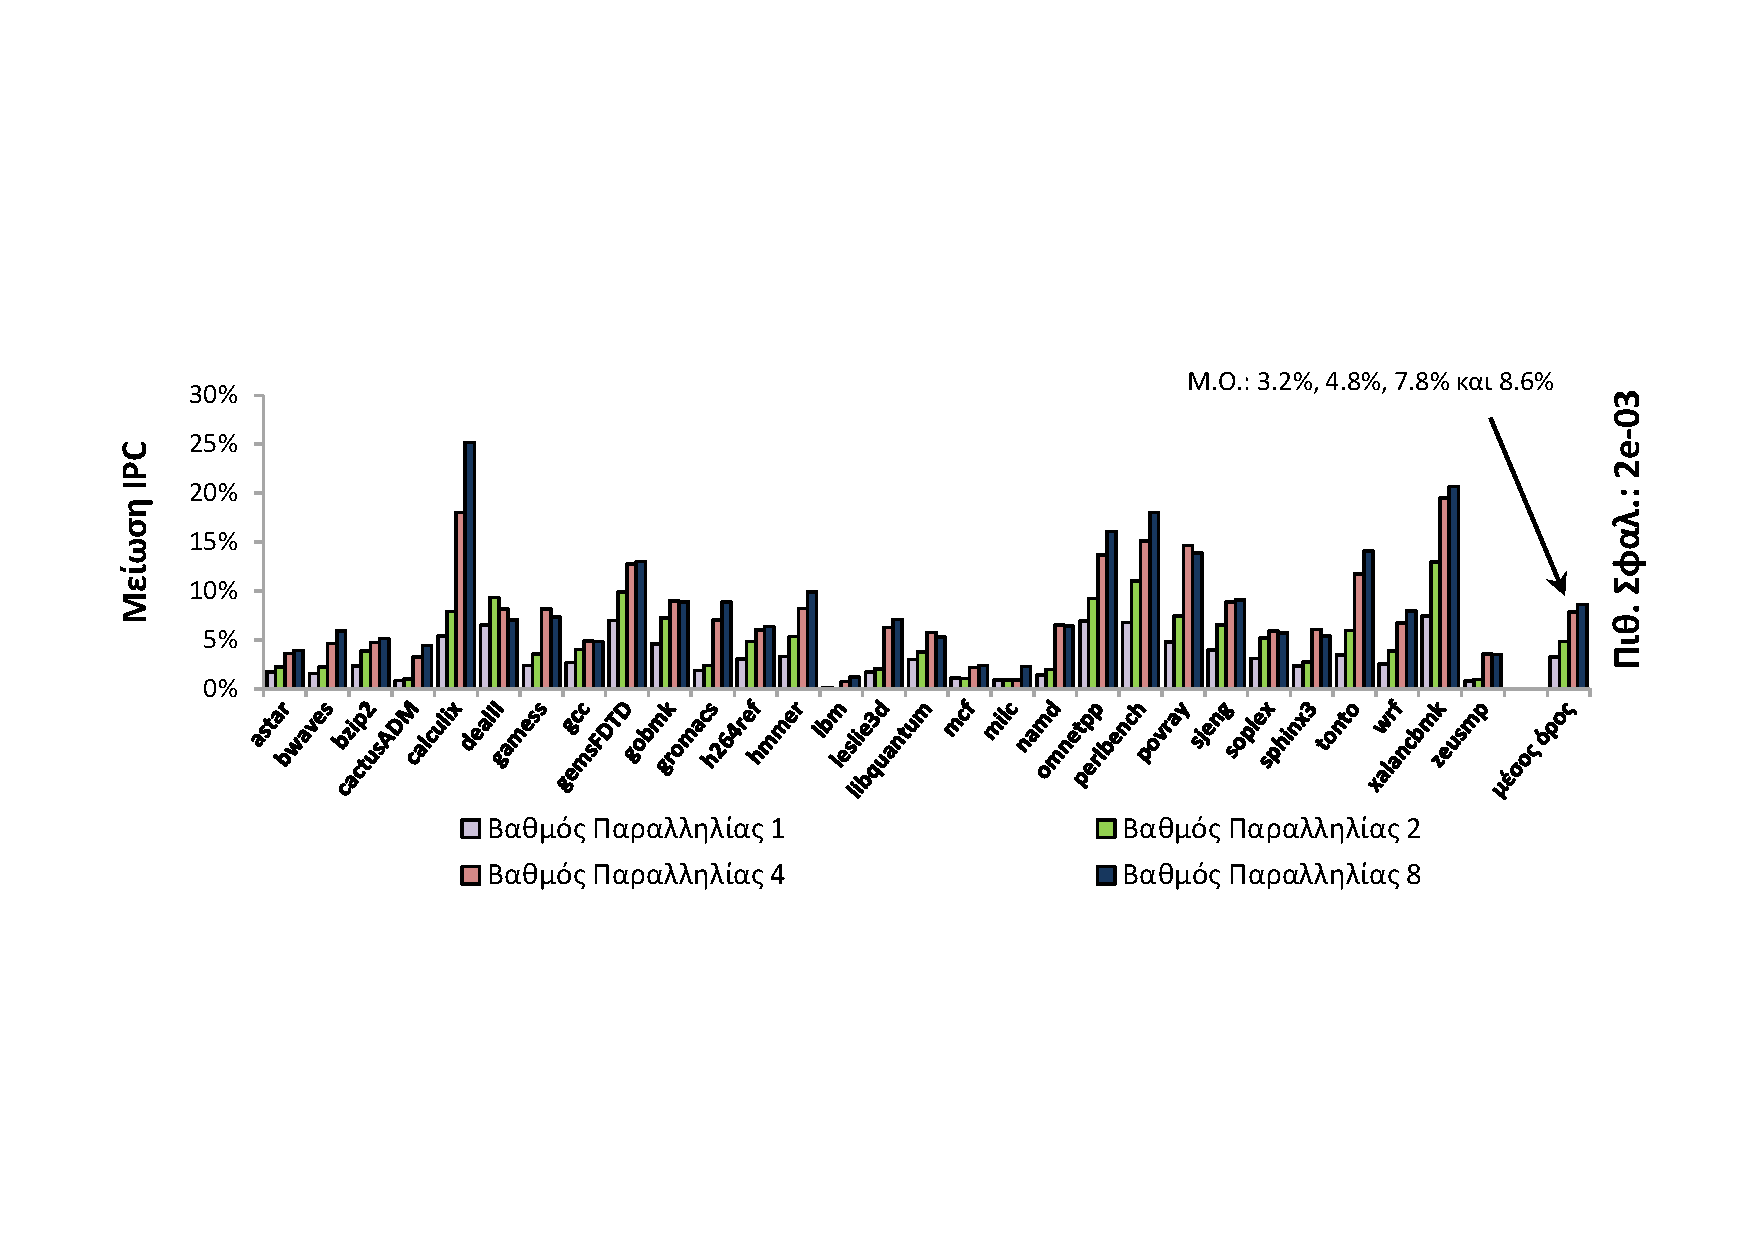
\includegraphics[width=\linewidth, trim=1.9cm 6.0cm 1.8cm 6.2cm, clip=true]{\resultsDIR/chap4_CORE_configs_ipc.pdf}}
    \caption{Μείωση του ρυθμού ολοκλήρωσης εντολών όταν υπάρχουν ελαττωματικά πλαίσια στον Πίνακα Πρόβλεψης Προορισμού Διακλάδωσης, για τέσσερα διαφορετικά μοντέλα εξομοιούμενων επεξεργαστών}
    \label{fig:chap4_core_config_performance}
\end{figure}

Ένα πολύ σημαντικό συμπέρασμα που μπορεί να εξαχθεί από το γράφημα του Σχήματος \ref{fig:chap4_core_config_performance}, είναι πως η επιρροή των σφαλμάτων της Μονάδας Δυναμικής Πρόβλεψης Διακλαδώσεων στην απόδοση γίνεται εντονότερη καθώς ο βαθμός παραλληλίας αυξάνεται. Συγκεκριμένα, στον επεξεργαστή βαθμού παραλληλίας 1 η μείωση της απόδοσης όταν στον Πίνακα Πρόβλεψης Προορισμού Διακλάδωσης υπάρχουν ελαττωματικά πλαίσια, είναι κατά μέσο όρο μόλις 3.2\%. Το ποσοστό αυτό ανεβαίνει σε 4.8\%, 7.8\% και 8.6\% με την αύξηση του βαθμού παραλληλίας αντίστοιχα. Το γεγονός αυτό είναι αναμενόμενο καθώς η προσκόμιση περισσότερων εντολών σε κάθε κύκλο ρολογιού συνεπάγεται και αύξηση των περιττών εντολών που θα προσκομιστούν στο Μηχανισμό Μερικώς Επικαλυπτόμενων Λειτουργιών, σε περίπτωση που υπάρξει λανθασμένη πρόβλεψη εντολής διακλάδωσης. Αυτό θα έχει ώς συνέπεια την εκτέλεση εντολών οι οποίες θα καταναλώσουν πολύτιμο χρόνο και ενέργεια έως ότου ανιχνευθεί η λανθασμένη πρόβλεψη, χωρίς να χρησιμοποιηθούν τελικώς τα αποτελέσματά τους. Για το λόγο αυτό δείχνει απαραίτητο να εξασφαλίζεται η κατά το δυνατόν αποδοτικότερη λειτουργία της Μονάδας Δυναμικής Πρόβλεψης Διακλαδώσεων σε επεξεργαστές που παρουσιάζουν αυξημένο βαθμό παραλληλίας.
\par
Οι τέσσερις περιπτώσεις διαφορετικών παραμέτρων που χρησιμοποιήθηκαν παρουσιάζονται στον Πίνακα \ref{tab:chap4_CoreConfigs}. Αναλυτικά δεδομένα για τα υπόλοιπα στοιχεία του μηχανισμού αναγράφονται στον Πίνακα \ref{tab:chap6_gem5parameters}, όπου περιγράφεται το γενικό μοντέλο που χρησιμοποιήθηκε κατά τη διαδικασίας της αξιολόγηση.

\begin{table}[!b]
    \centering
    %\begin{tabularx}{\textwidth}{!{\vrule width 4\arrayrulewidth} >{\centering\arraybackslash}X | >{\centering\arraybackslash}X !{\vrule width 4\arrayrulewidth}}
    \begin{tabularx}{\textwidth}{ >{\centering\arraybackslash}X >{\centering\arraybackslash}X }
    \Xhline{4\arrayrulewidth}
        \multirow{2}{*}{\textbf{Μοντέλο Εξομοίωσης}} & 
        \multirow{2}{\linewidth}{\centering \textbf{Παράμετροι (\en{Width/ROB/IQ/LQ/SQ/Registers})}} \\
        &    \\
        \Xhline{4\arrayrulewidth}
        {ΚΜΕ Βαθμού Παραλληλίας 1} & {1/32/16/16/16/64} \\
        %\hline
        {ΚΜΕ Βαθμού Παραλληλίας 2} & {2/64/32/32/32/64} \\
        %\hline
        {ΚΜΕ Βαθμού Παραλληλίας 4} & {4/128/64/64/64/128} \\
        %\hline
        {ΚΜΕ Βαθμού Παραλληλίας 8} & {8/256/256/128/128/128} \\
        \Xhline{4\arrayrulewidth}
    \end{tabularx}
    \caption{Παραμετροποιήσεις της Κεντρικής Μονάδας Επεξεργασίας}
    \label{tab:chap4_CoreConfigs}
\end{table}

%----------------------------------------------------------%

\section{Συμπεράσματα}
\label{chap4_FaultsAnalysisConclusions}

Παρότι στην Υποενότητα \ref{chap4_BTBConfigIPC} αναφέρθηκε πως η απόδοσης δεν επηρεάζεται αισθητά από το μέγεθος και την οργάνωση του Πίνακα Πρόβλεψης Προορισμού Διακλάδωσης, στην ανάλυση της Υποενότητας \ref{chap4_BranchTargetBufferFaults} παρουσιάζεται μία σημαντική πτώση του ρυθμού ολοκλήρωσης εντολών σε ορισμένες περιπτώσεις. Η αιτίας αυτής της πτώσης της απόδοσης είναι η εμφάνιση πλήρως ελαττωματικών συνόλων. Η αδυναμία αποθήκευσης πληροφορίας για ένα πλήθος εντολών διακλάδωσης θα έχει ώς συνέπεια την υποχρεωτική αναμονή (αδυναμία προσκόμισης νέων εντολών) έως τον υπολογισμό των αντίστοιχων διευθύνσεων προορισμού. Το κατά πόσο επηρεάζει ένα πλήρως ελαττωματικό σύνολο ένα εκτελούμενο πρόγραμμα εξαρτάται από τη διεύθυνση των εντολών διακλάδωσης καθώς, όπως αναφέρθηκε και στην Ενότητα \ref{chap2_BranchTargetBuffer}, η διευθυνσιοδότηση του συνόλου γίνεται από ένα τμήμα της διεύθυνσης εντολής. Επομένως, σε ορισμένες περιπτώσεις η επίδρασή των πλήρως ελαττωματικών συνόλων ενός συγκεκριμένου πίνακα στο χρόνο εκτέλεσης ενός προγράμματος μπορεί να είναι πολύ σημαντική, ενώ σε άλλες όχι.
\par
Γίνεται λοιπόν σαφές πως η ανάπτυξη κατάλληλης τεχνικής για τον περιορισμό των πλήρως ελαττωματικών συνόλων του Πίνακα Πρόβλεψης Προορισμού Διακλάδωσης θα περιόριζε σε μεγάλο βαθμό την αύξηση του χρόνου εκτέλεσης λόγω της εμφάνισης σφαλμάτων στη Μονάδα Δυναμικής Πρόβλεψης Διακλαδώσεων. Στην παρούσα μελέτη γίνεται η πρόταση μίας τέτοιας τεχνικής, η οποία είναι σε θέση να επιφέρει το επιθυμητό αποτέλεσμα σε μεγάλο βαθμό με το ελάχιστο δυνατό κόστος. Τόσο η υλοποίηση της προτεινόμενη τεχνικής όσο και τα αποτελέσματά της παρουσιάζονται στα ακόλουθα κεφάλαια.

%----------------------------------------------------------%

    \chapter{Λογική Μετάθεση Πλαισίων}
\label{chap5}

\section{Εισαγωγή}
\label{chap5_Intro}

Σύμφωνα με την έως τώρα ανάλυση, εξάγεται το συμπέρασμα πως η μείωση του αριθμού των πλήρως ελαττωματικών συνόλων θα συνέβαλε σημαντικά στη μείωση των επιπτώσεων που προκαλεί η ύπαρξη ελαττωματικών στοιχείων στον Πίνακα Πρόβλεψης Προορισμού Διακλάδωσης. Στο παρόν κεφάλαιο παρουσιάζεται μία νέα αυτοματοποιημένη τεχνική για την λογική μετάθεση των πλαισίων του πίνακα, με ελάχιστο κόστος. Η τεχνική αυτή συνοδεύεται από ένα αλγόριθμο ο οποίος παρουσιάζεται υπό δύο μορφές. Στην πρώτη μορφή του όλα τα βήματα εκτελούνται σειριακά, ενώ στη δεύτερη γίνεται χρήση παραλληλίας για ταχύτερο υπολογισμό.

%----------------------------------------------------------%

\section{Στόχος}
\label{chap5_Target}

Όπως αναφέρθηκε στο Κεφάλαιο \ref{chap2} ο Πίνακας Πρόβλεψης Προορισμού Διακλάδωσης, αποτελούνται από τ πλαίσια ανά σύνολο (Πλαίσιο-0 έως Πλαίσιο-[τ-1]) στα οποία συμπεριλαμβάνονται τα πεδία ετικέτας, διεύθυνσης προορισμού και ορισμένες επιπλέον πληροφορίες. Από την ανάλυση που έγινε στο Κεφάλαιο \ref{chap4} είναι φανερό πως η μείωση της επιβάρυνσης στην απόδοση εξαιτίας των σφαλμάτων στον Πίνακα Πρόβλεψης Προορισμού Διακλάδωσης μπορεί να επιτευχθεί μέσω του περιορισμού των πλήρως ελαττωματικών συνόλων, δηλαδή την καλύτερη κατανομή των ελαττωματικών πλαισίων ανάμεσα στα σύνολα.
\par
Στην ακόλουθη προτεινόμενη τεχνική, για την επίτευξη του στόχου χρησιμοποιείται η γνώση των θέσεων των ελαττωματικών πλαισίων του πίνακα, πληροφορία η οποία βρίσκεται αποθηκευμένη στα ψηφία σφάλματος. Οι τιμές αυτές εξάγονται μέσω της διαδικασίας ανίχνευσης λαθών στα στοιχεία μνήμης, όπως παρουσιάστηκε στο Κεφάλαιο \ref{chap3}, και αποθηκεύονται σε κατάλληλες δομές ώστε με τη μεταβολή της τάσης λειτουργίας να γίνεται και η ενημέρωση των αντίστοιχων ψηφίων σφάλματος. Για την καλύτερη επεξήγηση της τεχνικής ο πίνακας τ-τρόπων συνόλου συσχέτισης διαχωρίζεται σε τ τμήματα πλαισίων (Τμήμα-0 έως Τμήμα-[τ-1]). Έτσι το Τμήμα-0 θα περιέχει τα Πλαίσια-0 όλων των συνόλων, όπως παρουσιάζονται και στο Σχήμα \ref{fig:chap5_btb_init}.

\begin{figure}[t]
    \centering
    \fbox{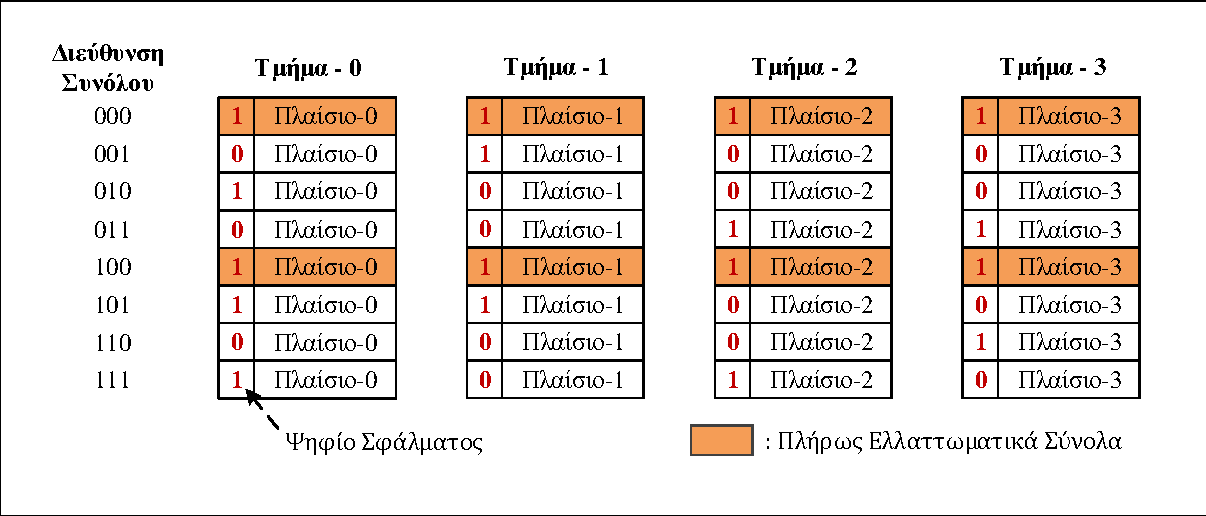
\includegraphics[width=\linewidth, trim=0.8cm 0.9cm 0.7cm 0.7cm, clip=true]{\algorithmsDIR/chap5_example.pdf}}
    \caption{Πλαίσια, σύνολα και τμήματα του Πίνακα Πρόβλεψης Προορισμού Διακλάδωσης}
    \label{fig:chap5_btb_init}
\end{figure}

Με βάση τις θέσεις των ελαττωματικών πλαισίων σε κάθε τμήμα, υπολογίζονται κατάλληλες τιμές οι οποίες αποθηκεύονται σε ένα ξεχωριστό καταχωρητή για κάθε τμήμα, τον αποκαλούμενο ως $``$Καταχωρητή Διαμόρφωσης$"$, ο οποίος χρησιμοποιείται για την τροποποίηση της διεύθυνσης πλαισίου του τμήματος. Η τελική διεύθυνση προσπέλασης (\textit{ΔΠ}) στην κάθε τμήμα παράγεται από τη συνάρτηση \xor μεταξύ του πεδίου διεύθυνσης (\textit{ΠΔ}) της εντολής διακλάδωσης και της τιμής του καταχωρητή διαμόρφωσης του τμήματος (\textit{ΚΔ}):
\begin{equation}
    \textit{ΔΠ(Τμήματος-Χ)} = \textit{ΠΔ} \oplus \textit{ΚΔ(Τμήματος-Χ)}
\end{equation}
\par
Με τον τρόπο αυτό γίνεται ανακατεύθυνση των προσπελάσεων με διαφορετικό τρόπο σε κάθε τμήμα δημιουργώντας έτσι νέα σύνολα πλαισίων τα οποία αποκαλούνται $``$Λογικά Σύνολα$"$. Σκοπός του αλγορίθμου που παρουσιάζεται στο παρόν κεφάλαιο είναι ο υπολογισμός κατάλληλων τιμών για τους Καταχωρητές Διαμόρφωσης, ώστε να επιτυγχάνεται η δημιουργία λογικών συνόλων με όσο το δυνατών λιγότερα πλήρως ελαττωματικά λογικά σύνολα. Για τη βελτίωση της απόδοσης, ο αλγόριθμος φροντίζει για τη συνολική βέλτιστη κατανομή των ελαττωματικών πλαισίων στα σύνολα, με κυρίαρχο στόχο την κατά το δυνατόν μέγιστη απαλοιφή των πλήρως ελαττωματικών συνόλων. Έτσι, σε ένα Πίνακα Πρόβλεψης Προορισμού Διακλάδωσης 4-τρόπων η σειρά προτεραιότητας στόχων είναι:

\begin{enumerate}[before=\itshape,font=\normalfont]
    \item Ελαχιστοποίηση λογικών συνόλων με 4 ελαττωματικά πλαίσια.
    \item Ελαχιστοποίηση λογικών συνόλων με 3 ελαττωματικά πλαίσια.
    \item Ελαχιστοποίηση λογικών συνόλων με 2 ελαττωματικά πλαίσια.
\end{enumerate}

Η προτεινόμενη τεχνική βασίζεται στην ιδέα εφαρμογής της θεωρίας των ορθογώνιων λατινικών τετραγώνων για την αντιμετώπιση των ελαττωμάτων της μνήμης που μελετώνται στα \cite{hsiao1975orthogonal} και \cite{bossen1984fault}.
\par
Στις ακόλουθες υπό ενότητες παρουσιάζονται δύο εκδοχές του αλγορίθμου. Η πρώτη εκτελεί σειριακά τον υπολογισμό κατάλληλων τιμών, ενώ η δεύτερη εκμεταλλεύεται τη δυνατότητα παραλληλίας. Από την πειραματική διαδικασία σε δείγμα 1000 χαρτών σφαλμάτων, αποδείχθηκε πως οι δύο τρόποι προσφέρουν παρεμφερές αποτέλεσμα κατά μέσο όρο.

%----------------------------------------------------------%

\section{Αλγόριθμοι Υπολογισμού Τιμών Μετάθεσης}
\label{chap5_Algorithms}

%----------------------------------------------------------%

\subsection{Σειριακός Αλγόριθμος}
\label{chap5_SerialAlgorithm}

\begin{algorithm}[H]
    \caption{\ \ \ Σειριακός Υπολογισμός Καταχωρητών Διαμόρφωσης}
    \label{alg:serial}
    \begin{algorithmic}[1]
        \begin{footnotesize}
            \Statex
            
            \Statex
            \begin{center}
                \textit{\textbf{Περιγραφή Μεταβλητών και Συναρτήσεων}}
            \end{center}
            
            \Statex
            \begin{description}[leftmargin=8em,style=nextline]
                \item [$SetsNumber$] Πλήθος συνόλων
                \item [$WaysNumber$] Πλήθος τμημάτων
                \item [$FaultMaps$] Θέσεις σφαλμάτων στη μνήμη (διεύθυνση συνόλου, τμήμα)
                \item [$S$] Αποδεκτές τιμές Καταχωρητών Διαμόρφωσης
                \item [$FB_{w}$] Διευθύνσεις ελαττωματικών πλαισίων στο τμήμα - \en{w}
                \item [$XFB_{w}$] Διευθύνσεις ελαττωματικών πλαισίων στο τμήμα - \en{w} μετά την εφαρμογή της νέας τιμής στον Καταχωρητή Διαμόρφωσης - \en{w}
                \item [$FS_{k}$] Διευθύνσεις λογικών συνόλων με \en{k} ελαττωματικά πλαίσια, μεταξύ των τμημάτων που έχουν συμμετάσχει έως το τρέχον βήμα του αλγορίθμου
                \item [$CCR$] Υποψήφιες τιμές του ελεγχόμενου Καταχωρητή Διαμόρφωσης μετά από κάθε βήμα του αλγορίθμου
                \item [$CR_{w}$] Τελική τιμή του Καταχωρητή Διαμόρφωσης - \en{w}
                \item [$COUNTER{[Y]}$] Μετρητές επανάληψης αποτελεσμάτων \en{Y} των λογικών πράξεων \xor\\ ($Y=0 \Rightarrow COUNTER[0]++$)
                \item[$elements(A)$] Συνάρτηση εύρεσης πλήθους στοιχείων του διανύσματος \en{A}
                \item[$minimum(A)$] Συνάρτηση εύρεσης μικρότερου στοιχείου του διανύσματος \en{A}
                \item[$random(A)$] Συνάρτηση τυχαίας επιλογής στοιχείου από το διάνυσμα \en{A}
            \end{description}
            
            \begin{center}
                \hrulefill
            \end{center}
            
            \selectlanguage{english}
            \Procedure {SerialPermutation}{$SetsNumber$, $WaysNumber$, $FaultMaps$}
                
                \\
                \State \Comment {\gr{Αρχικοποίηση}}
                \State $ maxAddress = SetsNumber - 1 $;
                \State $ S = \{ x\in \mathbb{R}, 0\le x\le maxAddress \} $;
                
                \\
                \For {$w = 0$ to $WaysNumber - 1$}
                    \State $ FB_{w} = \{ \textit{\gr{ελαττωματικές θέσεις τμήματος} - w} \} $;
                    \State $ XFB_{w} = \{ \emptyset \} $;
                    \State $ CR_{w} = 0 $;
                \EndFor
                
                \\
                \For {$b = 0$ to $WaysNumber$}
                    \State $ FS_{b} = \{ \emptyset \} $;
                \EndFor
                
                \\
                \State \linecomment{\gr{Αρχικά τα σύνολα με 1 ελαττωματικό πλαίσιο ταυτίζονται με αυτά του τμήματος 0}}
                \State $ FS_{1} =  FB_{0} $;
                \State $ FS_{0} =  S - FS_{1} $;
                \\
                %continue on next page
                \algstore{serial_alg_part1}
        \end{footnotesize}
    \end{algorithmic}
\end{algorithm}

\begin{algorithm}[H]
    \ContinuedFloat
    \caption{\ \ \ Σειριακός Υπολογισμός Καταχωρητών Διαμόρφωσης (Συνέχεια)}
    \begin{algorithmic}[1]
        \algrestore{serial_alg_part1}
        \begin{footnotesize}
            \selectlanguage{english}
                \State \Comment {\gr{Βήματα υπολογισμού κατάλληλης τιμής για κάθε καταχωρητή} w}
                \For {$w = 1$ to $WaysNumber - 1$}
                    
                    \State $ CCR = S $;
                    \State $ b = w $;
                    \While {$b > 0$}
                        \If {$ elements(CCR) > 1 $}
                            \\
                            \State $ COUNTER\left[ 0 : maxAddress \right] = 0 $;
                            \ForAll{$F_{R}$ in $FB_{w}$}
                                \ForAll{$F_{L}$ in $FS_{B}$}
                                    \State $ Y = F_{L} \oplus F_{R} $;
                                    \State $ COUNTER\left[ Y \right] = COUNTER\left[ Y \right] + 1 $;
                                \EndFor
                            \EndFor
                            \\
                            \State $ CAND\_CNT = \{ \emptyset \} $;
                            \ForAll{$CR$ in $CCR$}
                                \State $ CAND\_CNT = CAND\_CNT \cup COUNTER\left[ CR \right] $;
                            \EndFor
                            \\
                            \State $ MIN\_CNT = minimum(CAND\_CNT) $;
                            \State $ NEW\_CCR = \{ \emptyset \} $;
                            \ForAll{$CR$ in $CCR$}
                                \If {$ COUNTER\left[ CR \right] = MIN\_CNT$}
                                    \State $ NEW\_CCR = NEW\_CCR \cup CR $;
                                \EndIf
                            \EndFor
                            \\
                            \State $ CCR = NEW\_CCR $;
                            \\
                        \EndIf
                        \State $ b = b - 1 $;
                    \EndWhile
                    \\
                    \State $ CR_{w} = random(CCR) $;
                    \\
                    \ForAll{$F$ in $FB_{w}$}
                        \State $ XFB_{w} = XFB_{w} \cup (F \oplus CR_{w}) $;
                    \EndFor
                    \\
                    \State $ b = w + 1 $;
                    \While {$b > 0$}
                        \State $ FS_{b} = FS_{b} \cup (FS_{b-1} \cap XFB_{w}) $;
                        \State $ FS_{b-1} = FS_{b-1} - FS_{b} $;
                        \State $ b = b - 1 $;
                    \EndWhile
                    \\
                \EndFor
            \EndProcedure
        \end{footnotesize}
    \end{algorithmic}
\end{algorithm}


\subsubsection*{Παράδειγμα}

\begin{figure}[t]
    \centering
    \fbox{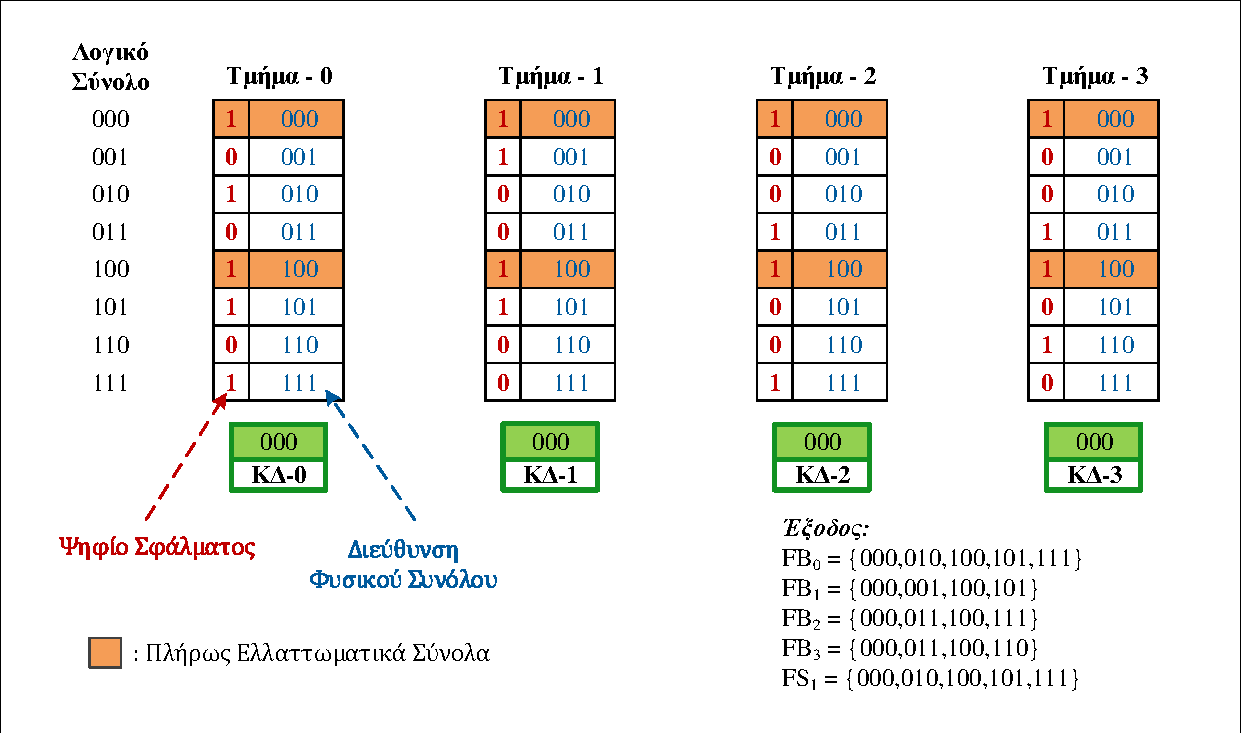
\includegraphics[width=\linewidth,trim=1cm 0.7cm 0.8cm 0.7cm, clip=true]{\algorithmsDIR/chap5_serial_example_step-0.pdf}}
    \caption{Αρχικοποίηση Σειριακού Αλγορίθμου}
    \label{fig:chap5_serial_init}
\end{figure}

Για την περιγραφή της μεθοδολογίας του σειριακού αλγορίθμου χρησιμοποιείται ένα παράδειγμα Πίνακα Πρόβλεψης Προορισμού Διακλάδωσης 4-τρόπων συνόλου συσχέτισης το οποίο παρουσιάζεται στο Σχήμα \ref{fig:chap5_serial_init}. Το πλήθος των σφαλμάτων δεν ανταποκρίνεται άμεσα στην πραγματικότητα αλλά διευκολύνει στην κατανόηση του τρόπου λειτουργίας του αλγορίθμου. Κάθε στοιχείο μιας στήλης του Σχήματος \ref{fig:chap5_serial_init} αποτελείται από δύο πεδία, το πρώτο υποδηλώνει εάν το πλαίσιο είναι ελαττωματικό ή όχι (1 ή 0 αντίστοιχα), ενώ το δεύτερο πεδίο υποδηλώνει τη φυσική διεύθυνση του πλαισίου. Όπως έχει ήδη αναφερθεί, η προτεινόμενη τεχνική υπολογίζει κατάλληλες τιμές για την επαναδιευθυνσιοδότηση των προσπελάσεων στον πίνακα, εκτελώντας την λογική πράξη \xor της αρχικής διεύθυνσης με μία τιμή μετάθεσης η οποία είναι αποθηκευμένη σε κατάλληλο καταχωρητή, δημιουργώντας έτσι τα λογικά σύνολα. Ένα λογικό σύνολο επομένως μπορεί να αποτελείται από ένα πλήθος πλαισίων είτε διαφορετικών είτε του ίδιου φυσικού συνόλου. Όταν οι τιμές των καταχωρητών είναι μηδενικές, τα λογικά και τα φυσικά σύνολα ταυτίζονται.
\par
Γνωρίζοντας τις θέσεις των ελαττωματικών πλαισίων κάθε τμήματος, στο βήμα της αρχικοποίησης καταγράφονται οι θέσεις αυτές σε τέσσερα διανύσματα αντίστοιχα: $FB_{0}$, $FB_{1}$, $FB_{2}$ και $FB_{3}$. Επίσης οι Καταχωρητές Διαμόρφωσης (ΚΔ) αρχικοποιούνται με τιμή 0, η οποία χρησιμοποιείται και στην κατάσταση κανονικής λειτουργίας όπου κανένα πλαίσιο δεν περιέχει ελαττωματικό δυαδικό ψηφίο. Επιπλέον, αρχικοποιείται το διάνυσμα $FS_{1}$ με τα περιεχόμενα του διανύσματος $FB_{0}$.

\begin{figure}[t]
    \centering
    \fbox{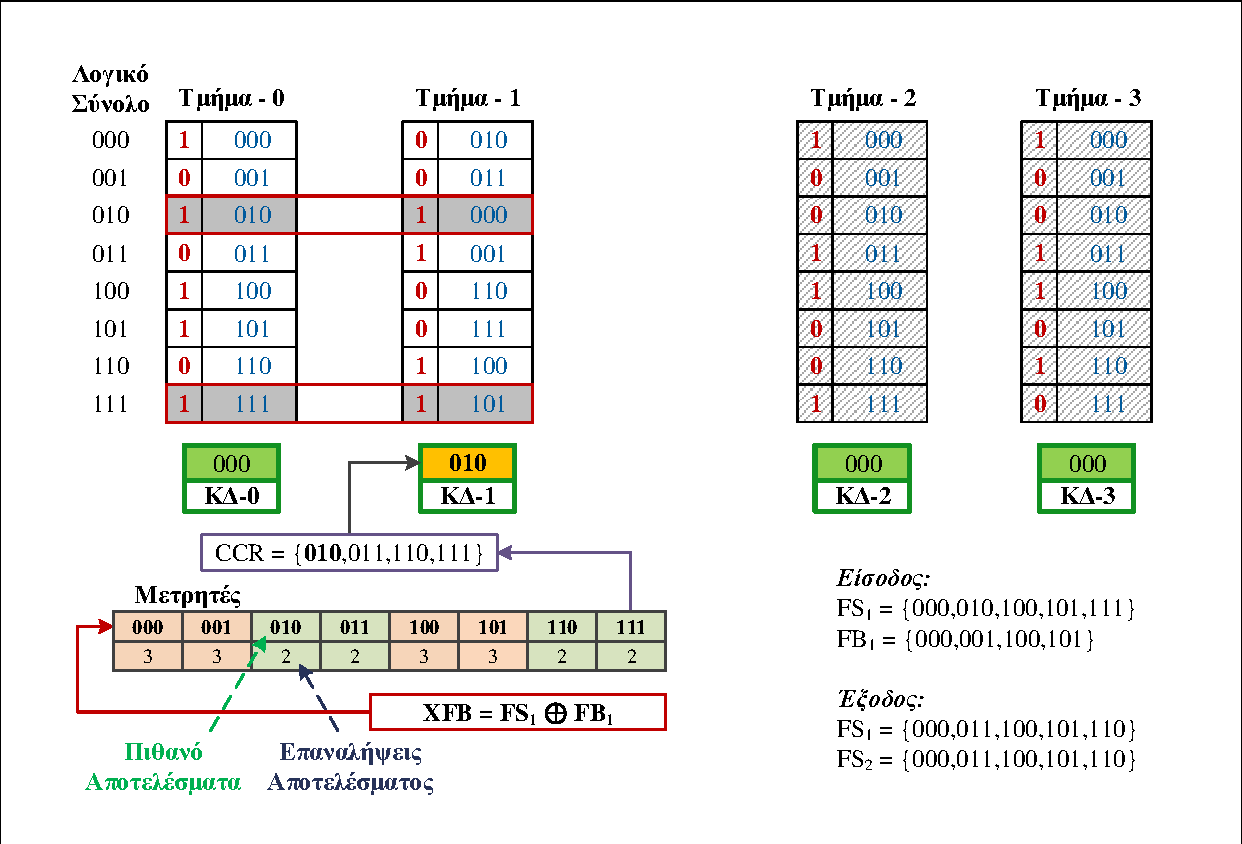
\includegraphics[width=\linewidth,trim=1cm 0.8cm 0.8cm 1cm, clip=true]{\algorithmsDIR/chap5_serial_example_step-1.pdf}}
    \caption{Σειριακό Βήμα 1\textsuperscript{ο} - Υπολογισμός ΚΔ-1}
    \label{fig:chap5_serial_step1}
\end{figure}

Στο πρώτο βήμα του αλγορίθμου, το οποίο παρουσιάζεται στο Σχήμα \ref{fig:chap5_serial_step1}, εκτελείται η συνάρτηση $XFB = FS_{1} \oplus FB_{1}$ για κάθε δυνατό συνδυασμό των περιεχομένων των δύο διανυσμάτων. Με τον υπολογισμό ενός αποτελέσματος γίνεται και η αύξηση του αντίστοιχου μετρητή. Κάθε μετρητής διατηρεί το ιστορικό εμφανίσεων ενός αποτελέσματος, όπως φαίνεται και στο Σχήμα \ref{fig:chap5_serial_step1}. Έτσι εάν το αποτέλεσμα της συνάρτησης είναι 0 η τιμή του μετρητής 0 αυξάνεται κατά ένα. Η πρώτη γραμμή του πίνακα μετρητών που παρουσιάζεται στο σχήμα περιέχει όλες τις δυνατές τιμές αποτελέσματος που μπορεί να πάρει η συνάρτηση:
\begin{equation}
    XFB = \{x \in \Re, 0 \leq x < 2^{log_2(\textit{πλήθος συνόλων})}\}
\end{equation}

Η δεύτερη γραμμή του πίνακα μετρητών περιέχει το άθροισμα των επαναλήψεων του αντίστοιχου αποτελέσματος, κατά τη διαδικασία εκτέλεσης των πράξεων \xor μεταξύ των στοιχείων των δύο διανυσμάτων. Συνεπώς, το άθροισμα των τιμών όλων των θέσεων της δεύτερης γραμμής πρέπει να ισούται με το γινόμενο του πλήθους των στοιχείων του πρώτου διανύσματος ($FS_{1}$) με το πλήθος των στοιχείων του δεύτερου διανύσματος ($FB_{1}$). Όσο δηλαδή ο συνολικός αριθμός λογικών πράξεων \xor που θα εκτελεστούν.
\par
Το πλήθος επαναλήψεων ενός αποτελέσματος, συνεπώς η τιμή του αντίστοιχου κελιού των μετρητών, υποδηλώνει πόσες περιπτώσεις θα παραμείνουν άλυτες μετά την εφαρμογή της συγκεκριμένης τιμής στον Καταχωρητή Διαμόρφωσης, δηλαδή πόσα λογικά σύνολα θα περιέχουν ελαττωματικά πλαίσια και στα δύο πρώτα τμήματα (Τμήμα-0 και Τμήμα-1). Επομένως, πρέπει να επιλεγεί η τιμή με το μικρότερο πλήθος επαναλήψεων.
\par
Από όλες τις δυνατές τιμές που μπορεί να λάβει ο \textit{ΚΔ-1}, επιλέγονται  αυτές με την ελάχιστη τιμή στον αντίστοιχο μετρητή. Οι επιλεγμένες τιμές αποθηκεύονται σε ένα διάνυσμα $CCR$ το οποίο δηλώνει τις εγκεκριμένες τιμές για τον καταχωρητή. Από τις τιμές που περιέχει το διάνυσμα $CCR$ επιλέγεται μία τυχαία η οποία αποθηκεύεται στον \textit{ΚΔ-1}. Σύμφωνα με τα περιεχόμενα των μετρητών του Σχήματος \ref{fig:chap5_serial_step1}, η καλύτερη λύση στο παρόν βήμα είναι η επιλογή μεταξύ των τιμών 010, 011, 110 και 111, ώστε να παραμείνουν δύο λογικά σύνολα με ελαττωματικά πλαίσια στο Τμήμα-0 και στο Τμήμα-1 ταυτόχρονα (για \textit{ΚΔ-1} = 010 $\Rightarrow$ λογικά σύνολα 010 και 111).
\par
Μετά την εφαρμογή της επιλεγμένης τιμής στον \textit{ΚΔ-1} εξάγονται δύο νέα διανύσματα. Το πρώτο διάνυσμα ($FS_{1}$) περιέχει τα σύνολα όπου μόνο ένα από τα δύο πλαίσια του λογικού συνόλου είναι ελαττωματικό, μεταξύ των δύο αυτών τμημάτων. Το δεύτερο διάνυσμα ($FS_{2}$) περιέχει τις θέσεις που και τα δύο πλαίσια είναι ελαττωματικά.

\begin{figure}[!b]
    \centering
    \fbox{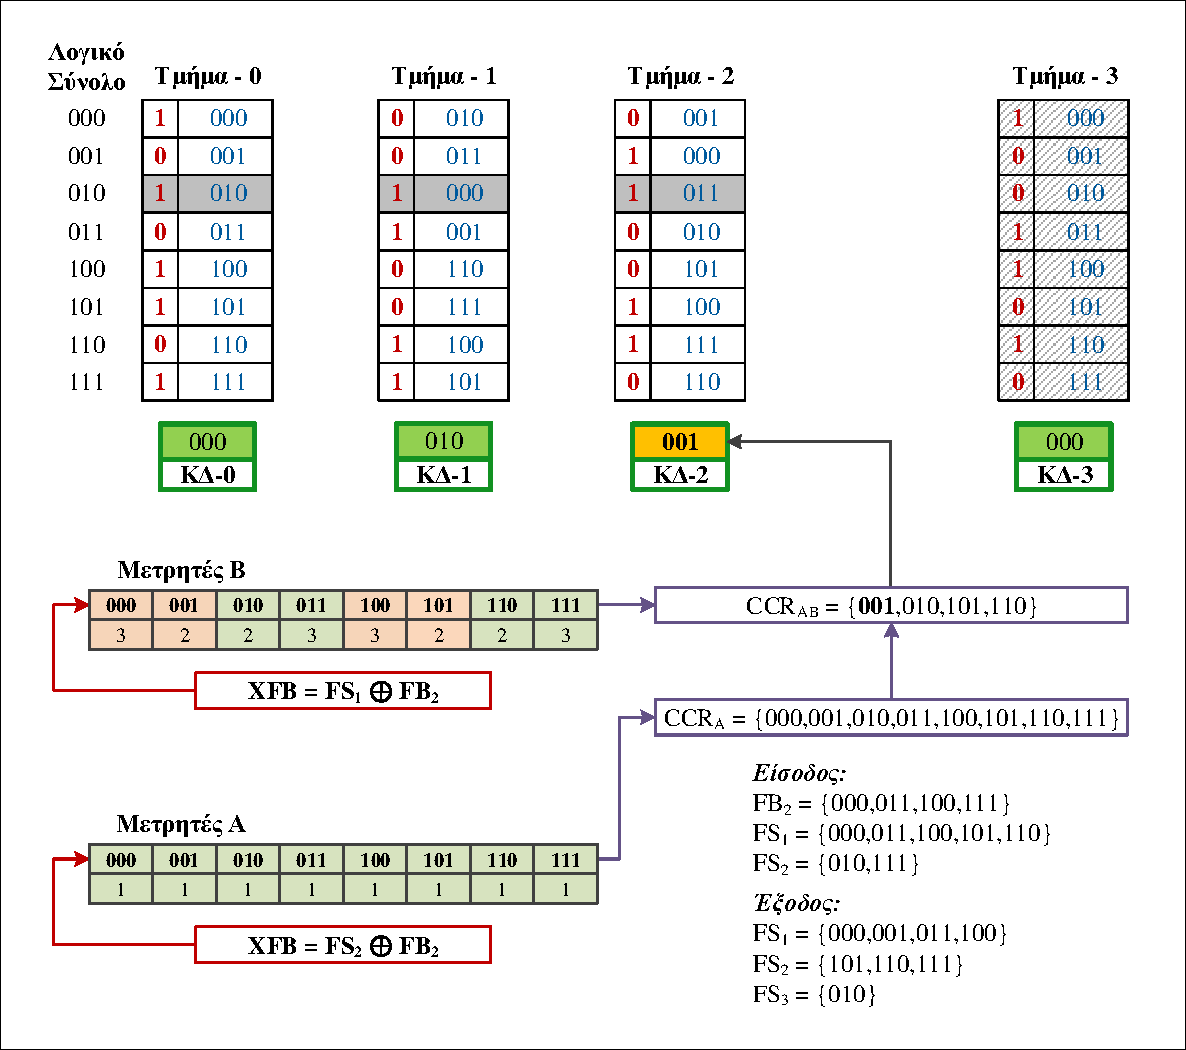
\includegraphics[width=\linewidth,trim=0.6cm 0.7cm 0.5cm 0.7cm, clip=true]{\algorithmsDIR/chap5_serial_example_step-2.pdf}}
    \caption{Σειριακό Βήμα 2\textsuperscript{ο} - Υπολογισμός ΚΔ-2}
    \label{fig:chap5_serial_step2}
\end{figure}

Κατά το δεύτερο βήμα, το οποίο παρουσιάζεται στο Σχήμα \ref{fig:chap5_serial_step2}, πρωταρχικός στόχος είναι η μείωση των λογικών συνόλων που θα περιέχουν 3 ελαττωματικά πλαίσια. Έτσι εκτελείται η συνάρτηση $XFB = FS_{2} \oplus FB_{2}$ για κάθε δυνατό συνδυασμό των περιεχομένων τους, καθώς και η αντίστοιχη αύξηση των μετρητών Α. Από όλες τις δυνατές τιμές που μπορεί να λάβει ο \textit{ΚΔ-2}, επιλέγονται αυτές με την ελάχιστη τιμή στον αντίστοιχο μετρητή. Οι επιλεγμένες αυτές τιμές αποθηκεύονται σε ένα διάνυσμα $CCR_{A}$.
\par
Δευτερεύων στόχος του αλγορίθμους σε αυτό το βήμα, είναι η μείωση των λογικών συνόλων που θα περιέχουν 2 ελαττωματικά πλαίσια. Για το λόγο αυτό, στη συνέχεια εκτελείται η συνάρτηση $XFB = FS_{1} \oplus FB_{2}$ με την αντίστοιχη ενημέρωση των μετρητών Β. Από τα στοιχεία που περιείχε το διάνυσμα $CCR_{A}$ επιλέγονται αυτά με τη μικρότερη τιμή στον πίνακα μετρητών Β. Τα επιλεγμένα στοιχεία αποθηκεύονται σε ένα διάνυσμα $CCR_{AB}$. Από το διάνυσμα αυτό επιλέγεται μία τιμή τυχαία η οποία αποθηκεύεται στον \textit{ΚΔ-2} (\textit{ΚΔ-2} = 001 στο παράδειγμα).
\par
Μετά την εφαρμογή της επιλεγμένης τιμής στον \textit{ΚΔ-2}, εξάγονται τρία νέα διανύσματα. Το πρώτο διάνυσμα ($FS_{1}$) περιέχει τα λογικά σύνολα που έχουν μόνο ένα από τα τρία πλαίσια ελαττωματικό, μεταξύ των τριών αυτών τμημάτων. Το δεύτερο διάνυσμα ($FS_{2}$) περιέχει τα σύνολα όπου δύο από τα τρία πλαίσια του λογικού συνόλου είναι ελαττωματικά. Το τρίτο διάνυσμα ($FS_{3}$) περιέχει τα σύνολα που και τα τρία πλαίσια είναι ελαττωματικά.

\begin{figure}[!b]
    \centering
    \fbox{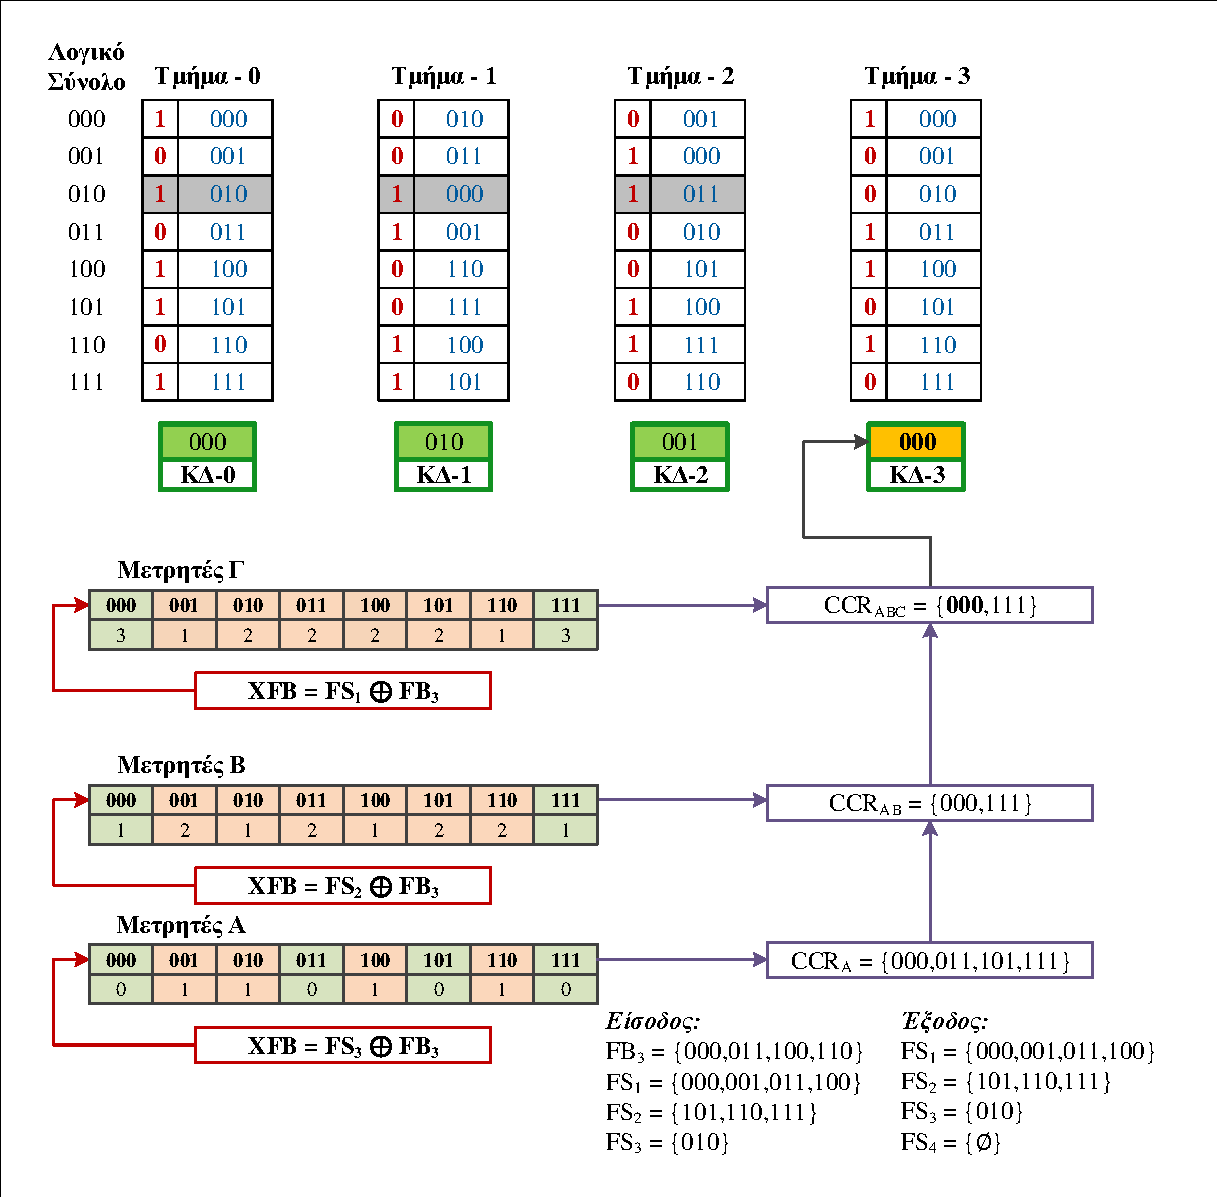
\includegraphics[width=\linewidth,trim=0.6cm 0.7cm 0.5cm 0.7cm, clip=true]{\algorithmsDIR/chap5_serial_example_step-3.pdf}}
    \caption{Σειριακό Βήμα 3\textsuperscript{ο} - Υπολογισμός ΚΔ-3}
    \label{fig:chap5_serial_step3}
\end{figure}

Κατά το τρίτο και τελευταίο βήμα, το οποίο παρουσιάζεται στο Σχήμα \ref{fig:chap5_serial_step3}, πρωταρχικός στόχος, ο οποίος αποτελεί και βασικό στόχο της προτεινόμενης τεχνικής, είναι η μείωση των λογικών συνόλων που θα περιέχουν 4 ελαττωματικά πλαίσια. Έτσι εκτελείται η συνάρτηση $XFB = FS_{3} \oplus FB_{3}$ για κάθε δυνατό συνδυασμό των περιεχομένων τους, με την αντίστοιχη αύξηση των μετρητών Α. Από όλες τις δυνατές τιμές που μπορεί να λάβει ο \textit{ΚΔ-3}, επιλέγονται αυτές με την ελάχιστη τιμή στον αντίστοιχο μετρητή και αποθηκεύονται σε ένα διάνυσμα $CCR_{A}$.
\par
Επόμενος στόχος του αλγορίθμους είναι η μείωση των λογικών συνόλων που θα περιέχουν 3 ελαττωματικά πλαίσια. Για το λόγο αυτό, εκτελείται η συνάρτηση $XFB = FS_{2} \oplus FB_{3}$ με την αντίστοιχη ενημέρωση των μετρητών Β. Από τα στοιχεία που περιείχε το διάνυσμα $CCR_{A}$ επιλέγονται αυτά με τη μικρότερη τιμή στον πίνακα μετρητών Β και αποθηκεύονται σε ένα νέο διάνυσμα $CCR_{AB}$.
\par
Τρίτος και με τη μικρότερη βαρύτητα στόχος του αλγορίθμους είναι η μείωση των λογικών συνόλων που θα περιέχουν 2 ελαττωματικά πλαίσια. Επομένως, εκτελείται η συνάρτηση $XFB = FS_{1} \oplus FB_{3}$ με την αντίστοιχη ενημέρωση των μετρητών Γ. Από τα στοιχεία που περιείχε το διάνυσμα $CCR_{AB}$ επιλέγονται αυτά με τη μικρότερη τιμή στον πίνακα μετρητών Γ και αποθηκεύονται σε ένα νέο διάνυσμα $CCR_{ABC}$. Από τις τιμές του διανύσματος αυτού επιλέγεται μία τυχαία η οποία αποθηκεύεται στον \textit{ΚΔ-3} (\textit{ΚΔ-3} = 000 στο παράδειγμα).
\par
Μετά την εφαρμογή της επιλεγμένης τιμής στον \textit{ΚΔ-3} εξάγονται τέσσερα νέα διανύσματα. Το πρώτο διάνυσμα ($FS_{1}$) περιέχει τα λογικά σύνολα όπου μόνο ένα από τα τέσσερα πλαίσια που το αποτελούν είναι ελαττωματικό. Το δεύτερο διάνυσμα ($FS_{2}$) τα λογικά σύνολα όπου δύο από τα τέσσερα πλαίσια είναι ελαττωματικά. Το τρίτο διάνυσμα ($FS_{3}$) τα λογικά σύνολα όπου τρία από τα τέσσερα πλαίσια είναι ελαττωματικά. Το τέταρτο διάνυσμα ($FS_{4}$) τα σύνολα όπου και τα τέσσερα πλαίσια είναι ελαττωματικά.
\par
Έπειτα από την εφαρμογή των νέων τιμών στους καταχωρητές διαμόρφωσης, όπως φανερώνεται και από το Σχήμα \ref{fig:chap5_serial_final}, τα πλήρως ελαττωματικά σύνολα έχουν εξαλειφθεί και η κατανομή των ελαττωματικών πλαισίων πλέον είναι πιο $``$δίκαιη$"$ μεταξύ των συνόλων.

\begin{figure}[h]
    \centering
    \fbox{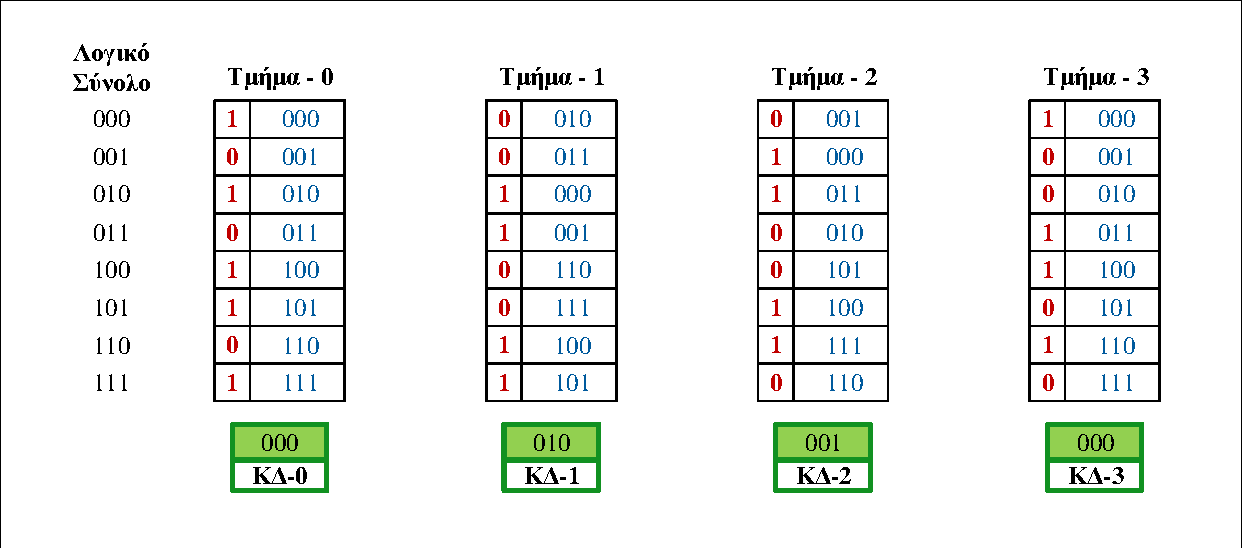
\includegraphics[width=\linewidth,trim=1cm 0.8cm 0.7cm 0.7cm, clip=true]{\algorithmsDIR/chap5_serial_example_step-final.pdf}}
    \caption{Λογικά σύνολα μετά την εκτέλεση του σειριακού αλγορίθμου}
    \label{fig:chap5_serial_final}
\end{figure}

%----------------------------------------------------------%

\subsection{Παράλληλος Αλγόριθμος}
\label{chap5_ParallelAlgorithm}

\begin{algorithm}[H]
    \captionsetup{}
    \caption{\ \ \ Παράλληλος Υπολογισμός Καταχωρητών Διαμόρφωσης}
    \label{alg:parallel}
    \begin{algorithmic}[1]
        \begin{footnotesize}
            \Statex 
            
            \Statex 
            \begin{center}
                \textit{\textbf{Περιγραφή Μεταβλητών και Συναρτήσεων}}
            \end{center}
            
            \Statex
            \begin{description}[leftmargin=9em,style=nextline]
                \item [$SetsNumber$] Πλήθος συνόλων
                \item [$WaysNumber$] Πλήθος τμημάτων
                \item [$FaultMaps$] Θέσεις σφαλμάτων στη μνήμη (διεύθυνση συνόλου, τμήμα)
                \item [$S$] Αποδεκτές τιμές Καταχωρητών Διαμόρφωσης
                \item [$FB_{w}$] Διευθύνσεις ελαττωματικών πλαισίων στο τμήμα - \en{w}
                \item [$XFB_{w}$] Διευθύνσεις ελαττωματικών πλαισίων στο τμήμα - \en{w} μετά την εφαρμογή της νέας τιμής στον Καταχωρητή Διαμόρφωσης - \en{w}
                \item [$FS_{[t,k]}$] Διευθύνσεις λογικών συνόλων με \en{k} ελαττωματικά πλαίσια, μεταξύ των τμημάτων που έχουν συμμετάσχει στο νήμα \en{t} έως το τρέχον βήμα του αλγορίθμου
                \item [$CCR$] Υποψήφιες τιμές του ελεγχόμενου Καταχωρητή Διαμόρφωσης μετά από κάθε βήμα του αλγορίθμου
                \item [$CR_{w}$] Τελική τιμή του Καταχωρητή Διαμόρφωσης - \en{w}
                \item [$COUNTER{[X,Y]}$] Μετρητές επανάληψης αποτελεσμάτων \en{Y} των λογικών πράξεων \xor. Κάθε γραμμή του πίνακα έχει διαφορετική βαρύτητα. Η ανώτερη γραμμή (μικρότερη τιμή του \en{X}) έχει τη μικρότερη βαρύτητα, ενώ η κατώτερη γραμμή (μεγαλύτερη τιμή του \en{X}) τη μεγαλύτερη βαρύτητα, στην επιλογή τιμών για τους Καταχωρητές Διαμόρφωσης.\\
                ($Y=0 \Rightarrow COUNTER[X,0]++$)
                \item[$elements(A)$] Συνάρτηση εύρεσης πλήθους στοιχείων του διανύσματος \en{A}
                \item[$minimum(A)$] Συνάρτηση εύρεσης μικρότερου στοιχείου του διανύσματος \en{A}
                \item[$random(A)$] Συνάρτηση τυχαίας επιλογής στοιχείου από το διάνυσμα \en{A}
            \end{description}
            
            \begin{center}
                \hrulefill
            \end{center}
            
            \selectlanguage{english}
            \Procedure {ParallelPermutation}{$SetsNumber$, $WaysNumber$, $FaultMaps$}
                \State \Comment {\gr{Αρχικοποίησης}}
                \State $ maxAddress = SetsNumber - 1 $;
                \State $ S = \{ x\in \mathbb{R}, 0\le x\le maxAddress \} $;
                \State $parallelSteps = log2(WaysNumber) - 1$;
                \State $threadsNumber = WaysNumber$;
                
                \\
                \For {$w = 0$ to $WaysNumber - 1$}
                    \State $ FB_{w} = \{ \textit{\gr{ελαττωματικά πλαίσια τμήματος}-w} \} $;
                    \State $ XFB_{w} = \{ \emptyset \} $;
                    \State $ CR_{w} = 0 $;
                \EndFor
                \For {$b = 0$ to $WaysNumber$}
                    \State $ FS_{[w,b]} = \{ \emptyset \} $;
                \EndFor
                
                \\
                \State \linecomment{\gr{Αρχικά τα σύνολα του νήματος} k \gr{με 1 ελαττωματικό πλαίσιο ταυτίζονται με αυτά του τμήματος} k}
                \State $ FS_{w,1} =  FB_{w} $;
                \State $ FS_{w,0} =  S - FS_{w,1} $;
                
                %continue on next page
                \algstore{parallel_alg_part1}
        \end{footnotesize}
    \end{algorithmic}
\end{algorithm}

\begin{algorithm}[H]
    \ContinuedFloat
    \caption{\ \ \ Παράλληλος Υπολογισμός Καταχωρητών Διαμόρφωσης (Συνέχεια)}
    \begin{algorithmic}[1]
        \algrestore{parallel_alg_part1}
        \begin{footnotesize}
            \selectlanguage{english}
                \State \Comment {\gr{Βήματα υπολογισμού κατάλληλης τιμής για κάθε καταχωρητή} w}
                
                \For {$pstep = 1$ to $parallelSteps$}
                    \State $ threadWays = WaysNumber/threads $;
                    \linecomment{\gr{πλήθος τμημάτων ανά νήμα}}
                    
                    \\
                    \State \linecomment{\gr{Εκτέλεση συνάρτησης} XOR \gr{μεταξύ των νημάτων} t \gr{και} t+1. \gr{Η τιμή που εξάγεται}}
                    \State \linecomment{\gr{μεταβάλει τις τιμές των καταχωρητών των τμημάτων που περιέχει το νήμα} t+1.}
                    \For {$t = 0$ to $threadsNumber$ step $2$}
                        \State $ COUNTER\left[0 : 2*threadWays, 0 : maxAddress \right] = 0 $;
                        
                        \\
                        \For {$i = threadWays$ to $1$ step $-1$}
                            \For {$j = threadWays$ to $1$ step $-1$}
                                \State $ X = i + j $;
                                \ForAll{$F_{R}$ in $FS_{[t,i]}$}
                                    \ForAll{$F_{L}$ in $FS_{[t+1,j]}$}
                                        \State $ Y = F_{L} \oplus F_{R} $;
                                        \State $ COUNTER\left[N, Y \right] = COUNTER\left[X, Y \right] + 1 $;
                                    \EndFor
                                \EndFor
                            \EndFor
                        \EndFor
                        
                        \\
                        \State \linecomment{\gr{Υπολογισμός του συνόλου υποψήφιων τιμών, κρατώντας σε κάθε επανάληψη αυτές}}
                        \State \linecomment{\gr{με την ελάχιστη τιμή στη γραμμή} X \gr{του πίνακα. Η αναζήτηση ξεκινάει από την}}
                        \State \linecomment{\gr{κατώτερη γραμμή η οποία έχει τη μεγαλύτερη βαρύτητα (στόχος είναι η μείωση}}
                        \State \linecomment{\gr{των συνόλων που περιέχουν πολλά ελαττωματικά πλαίσια).}}
                        \State $ CCR = S $;
                        \For {$X = 2*threadWays$ to $2$ step $-1$}
                            \If {$ elements(CCR) > 1 $}
                                
                                \\
                                \State $ CAND\_CNT = \{ \emptyset \} $;
                                \ForAll{$CR$ in $CCR$}
                                    \State $ CAND\_CNT = CAND\_CNT \cup COUNTER\left[X, CR \right] $;
                                \EndFor
                                \State $ MIN\_CNT = minimum(CAND\_CNT) $;
                                \State $ NEW\_CCR = \{ \emptyset \} $;
                                \ForAll{$CR$ in $CCR$}
                                    \If {$ COUNTER\left[X, CR \right] = MIN\_CNT$}
                                        \State $ NEW\_CCR = NEW\_CCR \cup CR $;
                                    \EndIf
                                \EndFor
                                
                                \\
                                \State $ CCR = NEW\_CCR $;
                            \EndIf
                        \EndFor
                        
                        \\
                        \State $ TCR = random(CCR) $;
                        \For {$w = (t+1)*threadWays$ to $(t+2)*threadWay - 1$}
                            \State $ CR_{w} = CR_{w} \oplus TCR $;
                        \EndFor
                %continue on next page
                \algstore{parallel_alg_part2}
        \end{footnotesize}
    \end{algorithmic}
\end{algorithm}

\begin{algorithm}[H]
    \ContinuedFloat
    \caption{\ \ \ \gr{Παράλληλος Υπολογισμός Καταχωρητών Διαμόρφωσης (Συνέχεια)}}
    \begin{algorithmic}[1]
        \algrestore{parallel_alg_part2}
        \begin{footnotesize}
            \selectlanguage{english}
                        \For {$w = threadWays$ to $0$ step $-1$}
                            \State $ XFS = \{ \emptyset \} $;
                            \ForAll{$F$ in $FS_{[t+1,w]}$}
                                \State $ XFS = XFS \cup (F \oplus TCR) $;
                            \EndFor
                            $ FS_{[t+1,w]} = XFS $
                        \EndFor
                    \EndFor
                    \ \linecomment{t = t + 2}
                    
                    \\
                    \For {$t = 0$ to $threadsNumber$ step $2$}
                        \For {$w = 2*threadWays$ to $0$ step $-1$}
                            \State $ NFS = \{ \emptyset \} $;
                        \EndFor
                    
                        \For {$i = threadWays$ to $0$ step $-1$}
                            \For {$j = threadWays$ to $0$ step $-1$}
                                \State $ X = i + j $;
                                \State $ NFS_{X} = NFS_{X} \cup (FS_{[t,i]} \cap FS_{[t+1,j]}) $;
                            \EndFor
                        \EndFor
                        
                        \For {$w = 2*threadWays$ to $1$ step $-1$}
                            $ FS_{[t/2,w]} = NFS_{w} $
                        \EndFor
                    \EndFor
                    
                    \State $threadsNumber = threadsNumber/2 $;
                    
                \EndFor
                \ \linecomment{pstep = pstep + 1}
                
                \For {$w = 0$ to $WaysNumber$}
                    \ForAll{$F$ in $FB_{w}$}
                        \State $ XFB_{w} = XFB_{w} \cup (F \oplus CR_{w}) $;
                    \EndFor
                \EndFor
            \EndProcedure
        \end{footnotesize}
    \end{algorithmic}
\end{algorithm}

\clearpage

\subsubsection*{Παράδειγμα}

\begin{figure}[t]
    \centering
    \fbox{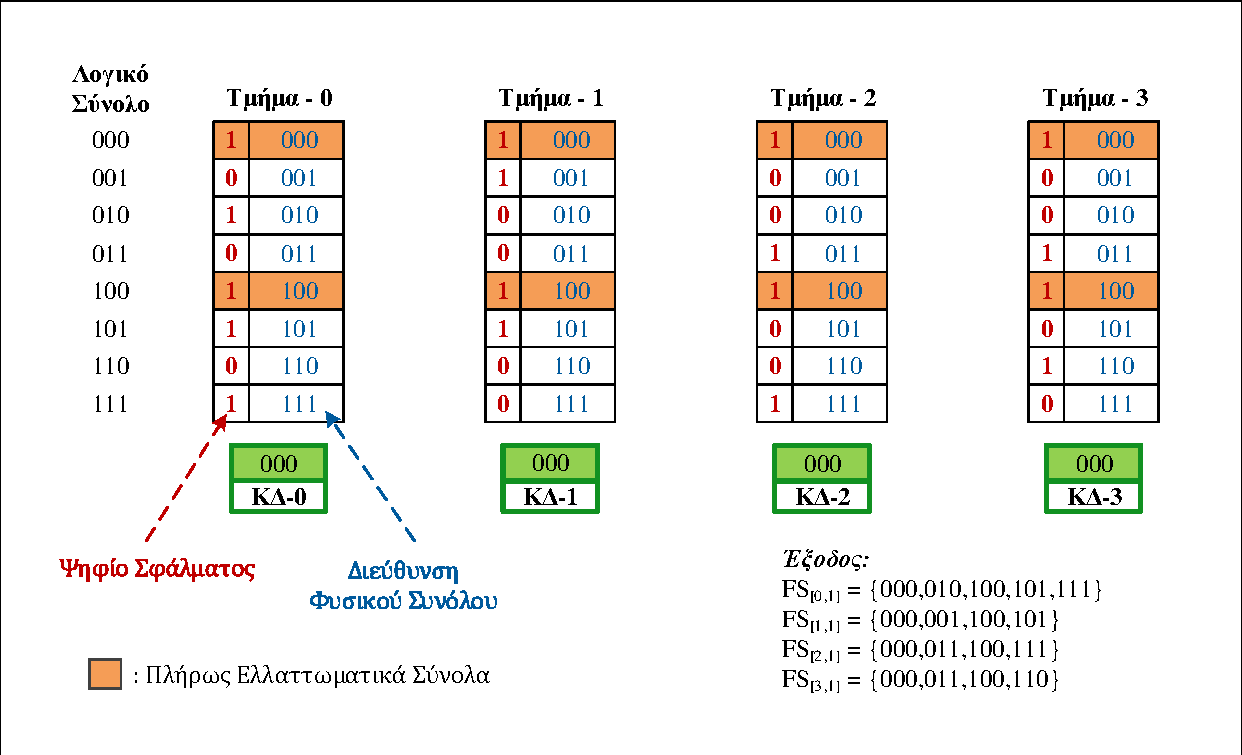
\includegraphics[width=\linewidth,trim=1cm 1cm 0.8cm 1cm, clip=true]{\algorithmsDIR/chap5_parallel_example_step-0.pdf}}
    \caption{Αρχικοποίηση Παράλληλου Αλγορίθμου}
    \label{fig:chap5_parallel_init}
\end{figure}

Για το παράδειγμα Πίνακα Πρόβλεψης Προορισμού Διακλάδωσης του σειριακού αλγορίθμου, αυτή τη φορά χρησιμοποιείται ο παράλληλος αλγόριθμος για τον υπολογισμό κατάλληλων τιμών των Καταχωρητών Διαμόρφωσης. Σε αντιστοιχία με τον σειριακό αλγόριθμο, κατά την αρχικοποίηση καταγράφονται οι θέσεις των ελαττωματικών πλαισίων των τεσσάρων τμημάτων στα αντίστοιχα διανύσματα: $FB_{0}$, $FB_{1}$, $FB_{2}$ και $FB_{3}$. Επίσης οι καταχωρητές αρχικοποιούνται με τιμή 0, όπως φανερώνει και το Σχήμα \ref{fig:chap5_parallel_init}.
\par
Θεωρώντας πως αρχικά κάθε τμήμα πλαισίων αντιστοιχεί σε ένα νήμα, ο αλγόριθμος υπολογισμού αποτελείται από στάδια παραλληλοποίησης όπου σε κάθε ένα από αυτά εκτελείται η συνάρτηση \xor μεταξύ δύο γειτονικών νημάτων. Στο τέλος της εκτέλεσης του σταδίου, γίνεται συνένωση των γειτονικών νημάτων σε ένα νέο νήμα (τα τ και τ+1 νήματα συνενώνονται). Στο επόμενο στάδιο ακολουθείται η ίδια διαδικασία για τα νέα μεγαλύτερα νήματα. Για κάθε νήμα εξάγονται κατάλληλα διανύσματα $FS_{[\mathgr{νήμα,ελαττωματικά πλαίσια συνόλου}]}$ που δηλώνουν τα λογικά σύνολα με τον αντίστοιχο αριθμό ελαττωματικών πλαισίων εντός του νήματος. Έτσι αρχικά για τα διανύσματα θα ισχύει: $FS_{[0,1]} = FB_{0}$, $FS_{[1,1]} = FB_{1}$, $FS_{[2,1]} = FB_{2}$ και $FS_{[3,1]} = FB_{3}$, όπως αναφέρεται και στο Σχήμα \ref{fig:chap5_parallel_init}.

\begin{figure}[t]
    \centering
    \fbox{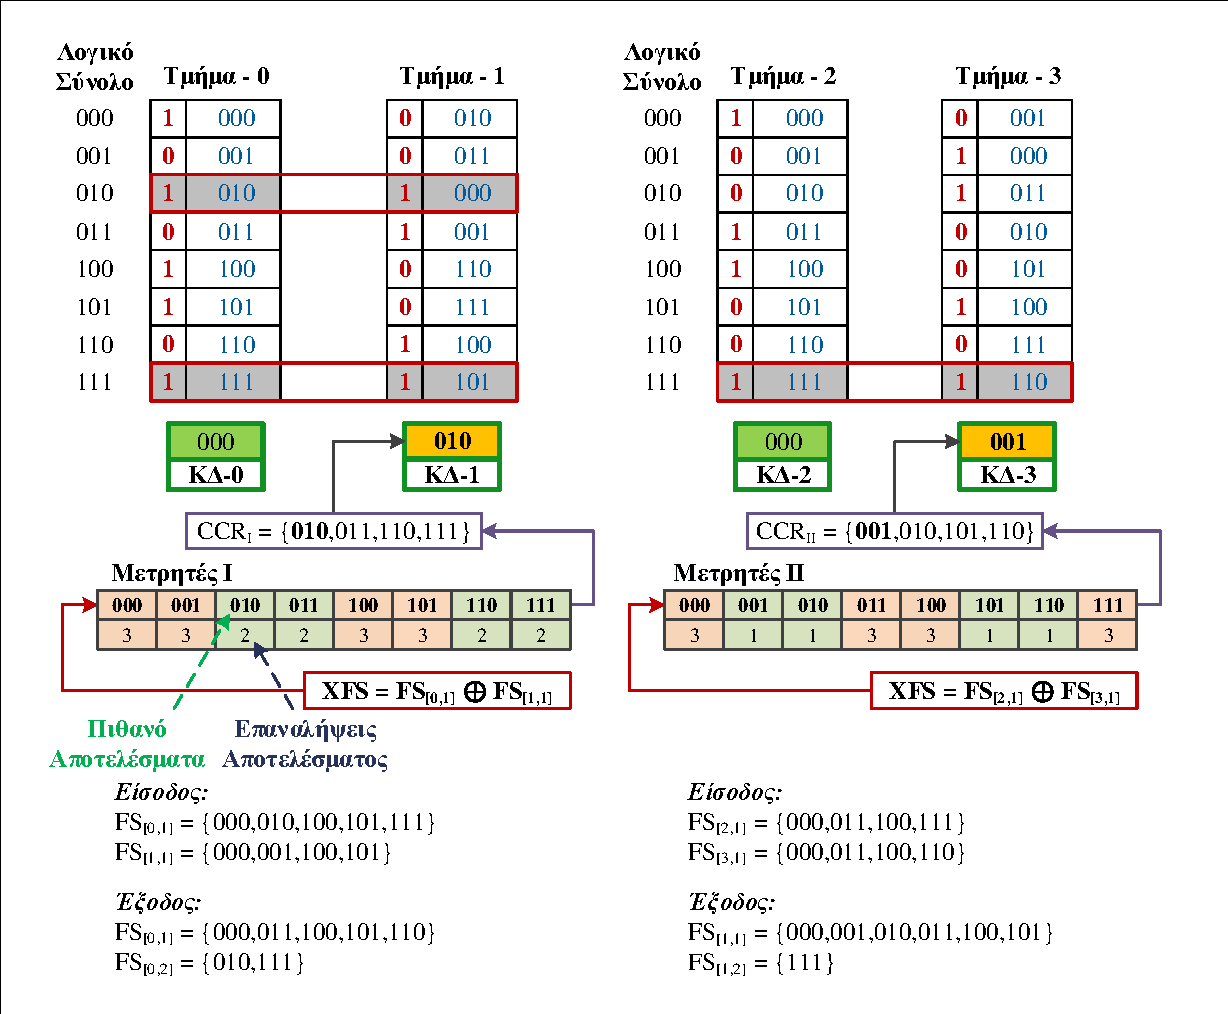
\includegraphics[width=\linewidth,trim=0.8cm 0.6cm 0.8cm 0.7cm, clip=true]{\algorithmsDIR/chap5_parallel_example_step-1.pdf}}
    \caption{Παράλληλο Βήμα 1\textsuperscript{ο} - Υπολογισμός ΚΔ-1 και KΔ-3}
    \label{fig:chap5_parallel_step1}
\end{figure}

Στο πρώτο βήμα του αλγορίθμου, εκτελούνται παράλληλα οι συναρτήσεις  $XFS = FS_{[0,1]} \oplus FS_{[1,1]}$  και $XFS = FS_{[2,1]} \oplus FS_{[3,1]}$, για κάθε δυνατό συνδυασμό των περιεχομένων των διανυσμάτων $FS$. Με την εκτέλεση κάθε πράξης γίνεται και η αύξηση του κατάλληλου μετρητή του αντίστοιχου ζεύγους νημάτων (μετρητές Ι και ΙΙ). Κάθε μετρητής διατηρεί το ιστορικό εμφανίσεων του αντίστοιχου αποτελέσματος, όπως φαίνεται και στο Σχήμα \ref{fig:chap5_parallel_step1}. Ακολουθώντας τη λογική του σειριακού αλγορίθμου, η δεύτερη γραμμή του πίνακα μετρητών περιέχει το πλήθος επαναλήψεων της αντίστοιχης τιμής ως αποτέλεσμα των λογικών συναρτήσεων \xor που εκτελούνται μεταξύ δύο γειτονικών τμημάτων (Τμήμα-0/Τμήμα-1 και Τμήμα-2/Τμήμα-3). Η τιμή μίας θέσης υποδηλώνει τον αριθμό των λογικών συνόλων που και στα δύο τμήματα τα πλαίσια που τα αποτελούν είναι ελαττωματικά, όταν στον Καταχωρητή Διαμόρφωσης του δεύτερου τμήματος κάθε ζεύγους νημάτων εφαρμοστεί η τιμή αυτή (\textit{ΚΔ-1} και \textit{ΚΔ-3} αντίστοιχα).
\par
Επομένως, από όλες τις δυνατές τιμές που μπορούν να λάβουν οι \textit{ΚΔ-1} και \textit{ΚΔ-3} επιλέγονται αυτές με την ελάχιστη τιμή στον αντίστοιχο μετρητή. Οι επιλεγμένες αυτές τιμές αποθηκεύονται στα διανύσματα $CCR_{I}$ και $CCR_{II}$. Από τα περιεχόμενα αυτών των διανυσμάτων, επιλέγεται μία τιμή τυχαία από κάθε ένα, η οποία αποθηκεύεται στους \textit{ΚΔ-1} και \textit{ΚΔ-3} αντίστοιχα (\textit{ΚΔ-1} = 010 και \textit{ΚΔ-3} = 001 στο παράδειγμα).
\par
Μετά την εφαρμογή της επιλεγμένης τιμής στους \textit{ΚΔ-1} και \textit{ΚΔ-3} εξάγονται δύο νέα διανύσματα για κάθε ζεύγος νημάτων. Το πρώτο διάνυσμα ($FS_{[0,1]}$ και $FS_{[1,1]}$ αντίστοιχα) περιέχει τις θέσεις όπου μόνο ένα από τα δύο πλαίσια είναι ελαττωματικό, μεταξύ των δύο τμημάτων που θα αποτελούν το νέο ενοποιημένο νήμα. Το δεύτερο διάνυσμα ($FS_{[0,2]}$ και $FS_{[1,2]}$ αντίστοιχα) περιέχει τις θέσεις όπου και τα δύο πλαίσια είναι ελαττωματικά.

\begin{figure}[!t]
    \centering
    \fbox{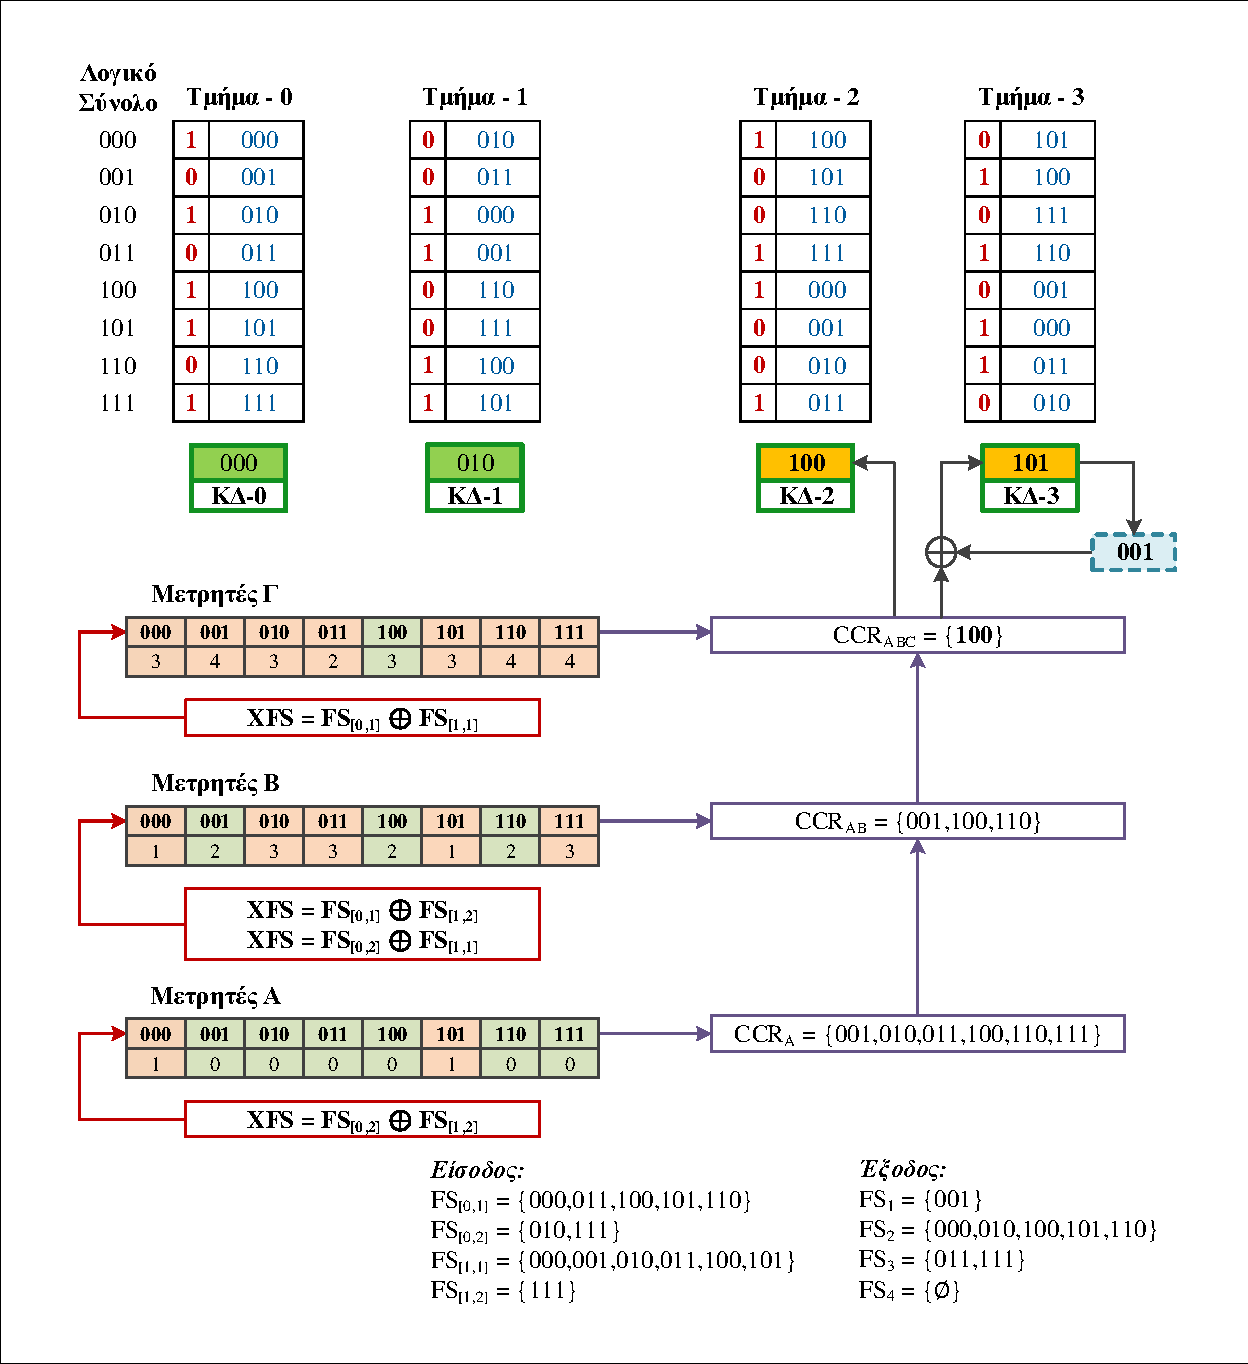
\includegraphics[width=\linewidth,trim=1cm 1cm 1cm 1cm, clip=true]{\algorithmsDIR/chap5_parallel_example_step-2.pdf}}
    \caption{Παράλληλο Βήμα 2\textsuperscript{ο} - Υπολογισμός ΚΔ-2 και ενημέρωση KΔ-3}
    \label{fig:chap5_parallel_step2}
\end{figure}

Κατά το δεύτερο βήμα, το οποίο απεικονίζεται στο Σχήμα \ref{fig:chap5_parallel_step2}, γίνεται ο υπολογισμός κατάλληλης τιμής του \textit{ΚΔ-2} και ενημέρωση του \textit{ΚΔ-3}. Κύριο στόχο αποτελεί η μείωση των λογικών συνόλων που θα περιέχουν 4 ελαττωματικά πλαίσια, συνεπώς εκτελείται η συνάρτηση $XFS = FS_{[0,2]} \oplus FS_{[1,2]}$ για κάθε δυνατό συνδυασμό των περιεχομένων αυτών των διανυσμάτων, καθώς και η αντίστοιχη αύξηση των μετρητών Α. Από όλες τις δυνατές τιμές που μπορεί να λάβει ο \textit{ΚΔ-2} επιλέγονται αυτές με την ελάχιστη τιμή στον αντίστοιχο μετρητή. Οι επιλεγμένες τιμές αποθηκεύονται σε ένα διάνυσμα $CCR_{A}$.
\par
Εφόσον έχει εξασφαλιστεί στο μέγιστο δυνατό η επίλυση του πρώτου στόχου, ο αλγόριθμος αναζητά και τη μείωση των λογικών συνόλων που θα περιέχουν 3 ελαττωματικά πλαίσια. Για το λόγο αυτό εκτελούνται οι συναρτήσεις $XFS = FS_{[0,1]} \oplus FS_{[1,2]}$ και $XFS = FS_{[0,2]} \oplus FS_{[1,1]}$ με κατάλληλη ενημέρωση των κοινών μετρητών Β. Από τα στοιχεία που περιείχε το διάνυσμα $CCR_{A}$ επιλέγονται αυτά με τη μικρότερη τιμή στον πίνακα μετρητών Β και αποθηκεύονται σε ένα νέο διάνυσμα $CCR_{AB}$.
\par
Έχοντας ολοκληρώσει τους δύο πρώτους στόχους, ο αλγόριθμος ελέγχει τη δυνατότητα μείωσης των λογικών συνόλων που θα περιέχουν 2 ελαττωματικά πλαίσια. Ο έλεγχος αυτός γίνεται μέσω της εκτέλεσης της συνάρτησης $XFS = FS_{[0,1]} \oplus FS_{[1,1]}$ με την αντίστοιχη ενημέρωση των μετρητών Γ. Από τα στοιχεία που περιείχε το διάνυσμα $CCR_{AB}$ επιλέγονται αυτά με τη μικρότερη τιμή στον πίνακα μετρητών Γ και αποθηκεύονται σε ένα νέο διάνυσμα $CCR_{ABC}$.
\par
Από τις τιμές που θα καταλήξουν στο διάνυσμα $CCR_{ABC}$ επιλέγεται μία τυχαία, η οποία γίνεται \xor με τις προηγούμενες τιμές των \textit{ΚΔ-2} και \textit{ΚΔ-3} και τα αποτελέσματά των συναρτήσεων αποθηκεύονται στους αντίστοιχους Καταχωρητές Διαμόρφωσης. Έτσι θα έχουμε τις νέες τιμές \textit{ΚΔ-2’ = ΚΔ-2} $\oplus$ $CCR$ και \textit{ΚΔ-3’ = ΚΔ-3} $\oplus$ $CCR$ (\textit{ΚΔ-2} = 100 και \textit{ΚΔ-3} = 101 στο παράδειγμα).
\par
Μετά την εφαρμογή των επιλεγμένων τιμών στους \textit{ΚΔ-2} και \textit{ΚΔ-3}, εξάγονται τέσσερα νέα διανύσματα. Το πρώτο διάνυσμα ($FS_{1}$) περιέχει τα λογικά σύνολα όπου μόνο ένα από τα τέσσερα πλαίσια είναι ελαττωματικό. Το δεύτερο διάνυσμα ($FS_{2}$) τα λογικά σύνολα όπου δύο από τα τέσσερα πλαίσια είναι ελαττωματικά. Το τρίτο διάνυσμα ($FS_{3}$) τα λογικά σύνολα όπου τρία από τα τέσσερα πλαίσια είναι ελαττωματικά. Το τέταρτο διάνυσμα ($FS_{4}$) τα λογικά σύνολα όπου και τα τέσσερα πλαίσια είναι ελαττωματικά.
\par
Με την εφαρμογή των νέων τιμών στους καταχωρητές διαμόρφωσης, όπως φανερώνει και το Σχήμα \ref{fig:chap5_parallel_final}, το αποτέλεσμα είναι παρόμοιο με τον σειριακό αλγόριθμο καθώς τα πλήρως ελαττωματικά σύνολα έχουν εξαλειφθεί.

\begin{figure}[h]
    \centering
    \fbox{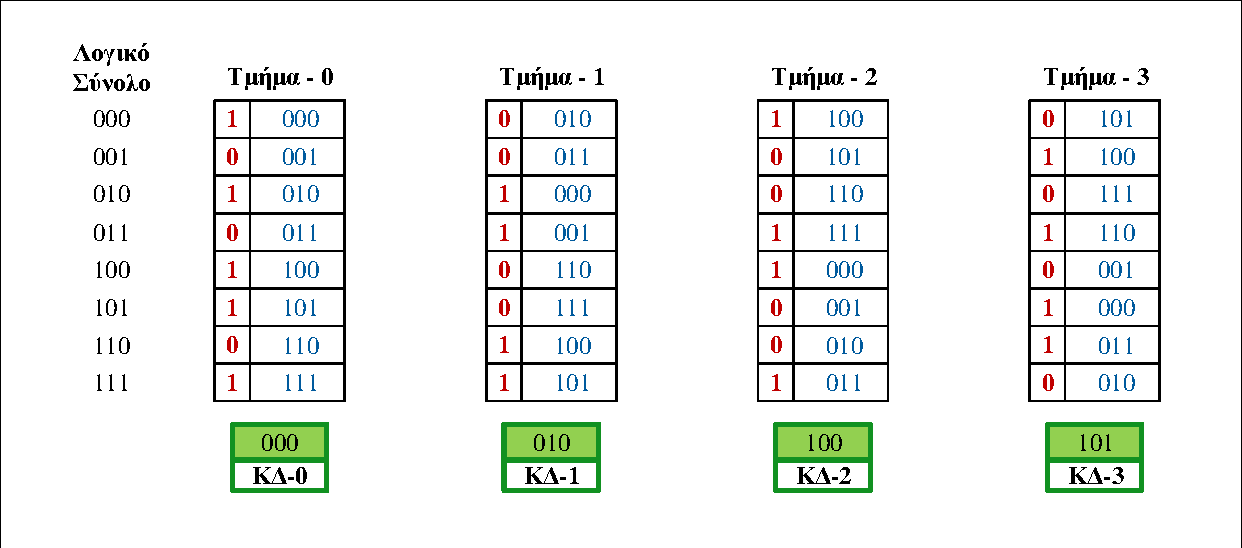
\includegraphics[width=\linewidth,trim=1cm 0.8cm 0.7cm 0.7cm, clip=true]{\algorithmsDIR/chap5_parallel_example_step-final.pdf}}
    \caption{Λογικά σύνολα μετά την εκτέλεση του παράλληλου αλγορίθμου}
    \label{fig:chap5_parallel_final}
\end{figure}

%----------------------------------------------------------%

\section{Βελτιστοποίηση}
\label{chap5_ImprovedMethod}

Όπως θα αποδειχθεί και από την πειραματική αξιολόγηση της τεχνικής που πραγματοποιείται στην Ενότητα \ref{chap5_AlgorithmResults}, ο τρόπος λειτουργίας της προτεινόμενης τεχνικής σε συνδυασμό με την τυχαιότητα των θέσεων των ελαττωματικών κυψελίδων, σε ορισμένες περιπτώσεις καθιστά αδύνατη την ολοκληρωτική εξάλειψη των πλήρως ελαττωματικών συνόλων. Στη μορφή της τεχνικής που παρουσιάστηκε έως τώρα η διεύθυνση προσπέλασης σε κάθε τμήμα πλαισίων μεταβάλετε από έναν και μόνο καταχωρητή. Το γεγονός αυτό δεν επιτρέπει την διαφοροποίηση του τρόπου μετάθεσης μεταξύ τμημάτων των τμημάτων. Για παράδειγμα, ένας επιθυμητός τρόπος μεταβολής της διεύθυνσης στο Τμήμα-0 θα μπορούσε να είναι ο ακόλουθος:
\begin{enumerate}[itemsep=0.5pt]
    \item Σύνολα 000 έως 011 $\Longrightarrow$ \xor με την τιμή 010
    \item Σύνολα 100 έως 111 $\Longrightarrow$ \xor με την τιμή 001
\end{enumerate}

Η λύση για την επίτευξη αυτού του αποτελέσματος έρχεται από τη διάσπαση των τμημάτων πλαισίων σε υποτμήματα, με τη χρήση περισσότερων Καταχωρητών Διαμόρφωσης ανά τμήμα, όπως παρουσιάζεται στο Σχήμα \ref{fig:chap5_multiCR_init}, για το παράδειγμα του σειριακού αλγορίθμου.

\begin{figure}[!t]
    \centering
    \fbox{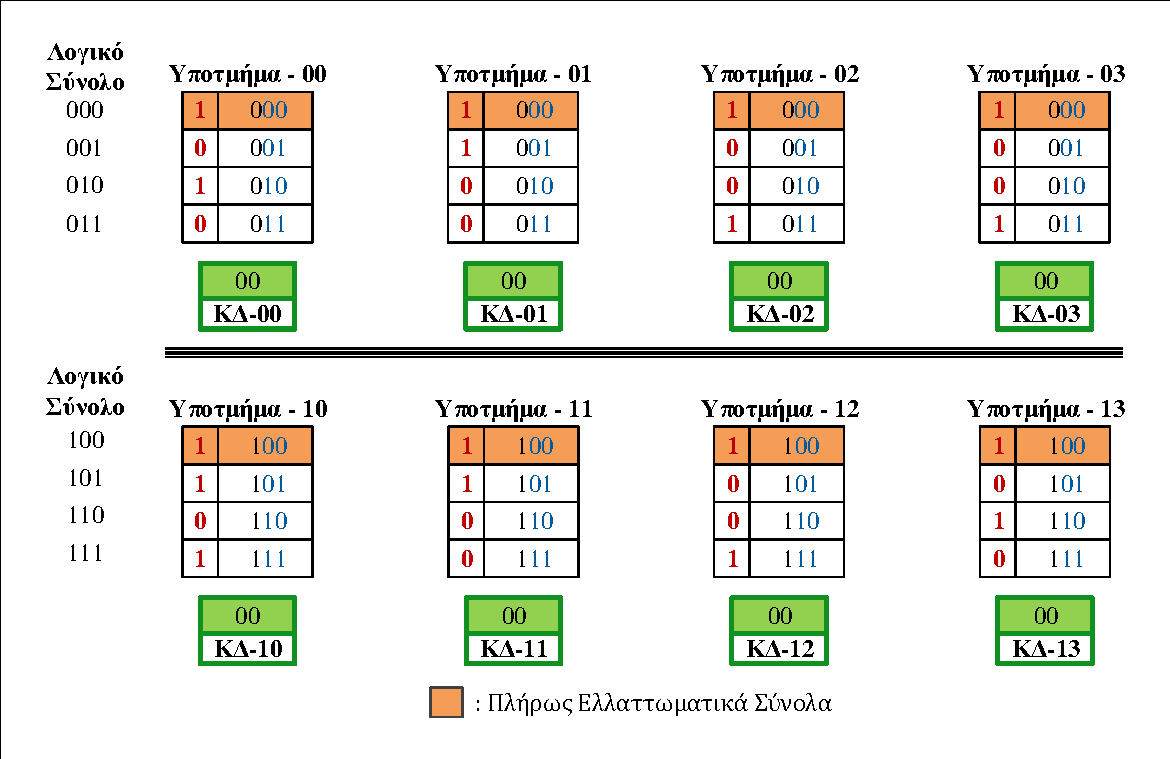
\includegraphics[width=\linewidth,trim=0.5cm 0.7cm 0.5cm 0.7cm, clip=true]{\algorithmsDIR/chap5_multiCR_example_step-0.pdf}}
    \caption{Μορφή βελτιστοποιημένης τεχνικής}
    \label{fig:chap5_multiCR_init}
\end{figure}

Κάθε Υποτμήμα-Χ αποτελείται από ένα πλήθος Πλαισίων-Χ συνεχόμενων συνόλων και διαθέτει ξεχωριστό Καταχωρητή Διαμόρφωσης. Επομένως, στο παράδειγμα του σχήματος όπου ο Πίνακας Πρόβλεψης Προορισμού Διακλάδωσης αποτελείται από 4 τμήματα με 2 υποτμήματα το κάθε ένα, ο συνολικός αριθμός απαιτούμενων καταχωρητών είναι 8 ($4\times2$). Ο αλγόριθμος για τον υπολογισμό τιμών εκτελείται ανεξάρτητα για κάθε τμήμα συνόλων. Αρχικά εκτελείται μεταξύ των υποτμημάτων που αποτελούνται από τα σύνολα $000$ έως $011$ (υποτμήματα 00, 01, 02, 03), και στη συνέχεια για τα υποτμήματα που αποτελούνται από τα σύνολα $100$ έως $111$ (υποτμήματα 10, 11, 12, 13). Η παραγόμενη τιμή θα αποτελείται από δύο δυαδικά ψηφία, καθώς το πιο σημαντικό δυαδικό ψηφίο της διεύθυνσης λογικού συνόλου παραμένει αναλλοίωτο (ισούται με το πιο σημαντικό ψηφίο της διεύθυνσης φυσικού συνόλου). Τέλος, για τον υπολογισμό κατάλληλων τιμών χρησιμοποιείται ο σειριακός αλγόριθμος καθώς σε ορισμένες περιπτώσεις κατανομής σφαλμάτων λειτουργεί αποδοτικότερα.

%----------------------------------------------------------%

\section{Στοιχεία Επίτευξης Στόχου}
\label{chap5_AlgorithmResults}

Για την εκτίμηση της απόδοσης της τεχνικής ως προς την επίτευξη του αρχικού στόχου, δηλαδή την ικανότητά της να μειώνει τα πλήρως ελαττωματικά σύνολα στο μέγιστο δυνατό, πραγματοποιήθηκε πειραματική αξιολόγηση σε δείγμα 1000 χαρτών σφαλμάτων. Στα γραφήματα που ακολουθούν, οι δείκτες πράσινων, πορτοκαλί, μπλε, κόκκινων και γκρι αποχρώσεων ισοδυναμούν με τα αποτελέσματα για πιθανότητες σφάλματος $\expnum{1}$, $\expnum{2}$, $\expnum{3}$, $\expnum{4}$ και $\expnum{5}$ αντίστοιχα. Η μείωση του πλήθους πλήρως ελαττωματικών συνόλων (ΠΕΣ) ορίζεται ως:
\begin{equation}
    \label{eqn:chap5_FFSETS}
    \mathgr{Μείωση\_ΠΕΣ} = \frac{\mathgr{ΠΕΣ}_\mathgr{αρχικά} - \mathgr{ΠΕΣ}_\mathgr{με\_τεχνική\_μετάθεσης}}{\mathgr{ΠΕΣ}_\mathgr{αρχικά}}
\end{equation}

Στο Σχήμα \ref{fig:chap5_btb_ffsets_2048} παρουσιάζονται τα αποτελέσματα των διαφορετικών παραλλαγών της τεχνικής για την περίπτωσης ένα Πίνακα Πρόβλεψης Προορισμού Διακλάδωσης (ΠΠΠΔ) 2048 πλαισίων, 2 και 4-τρόπων συνόλου συσχέτισης. Στο Σχήμα \ref{fig:chap5_btb_ffsets_2048_2way} όπου παρουσιάζονται τα αποτελέσματα του πίνακα 2048-πλαισίων/2-τρόπων, κάθε σημείο του οριζόντιου άξονα αντιστοιχεί στο πλήθος καταχωρητών ανά τμήμα. Συνεπώς, το πρώτο σημείο κάθε καμπύλης αντιστοιχεί στην εφαρμογή του κλασικού σειριακού αλγορίθμου. Όπως ήταν αναμενόμενο από την επεξήγηση που δόθηκε στην Ενότητα \ref{chap5_ImprovedMethod}, η χρήση ενός μόνο καταχωρητή ανά τμήμα περιορίζει αρκετά τη δυνατότητα αναδιανομή των ελαττωματικών πλαισίων στα σύνολα.
\par
Με τη διάσπαση των τμημάτων σε υποτμήματα, όπως φαίνεται και στο γράφημα, παρουσιάζεται σημαντική βελτίωση της απόδοσης της τεχνικής. Στην πιθανότητα σφάλματος $\expnum{1}$ η χρήση 4 καταχωρητών ανά τμήμα είναι αρκετή για να επιφέρει την ολοκληρωτική εξάλειψη των πλήρως ελαττωματικών συνόλων. Για την πιθανότητα σφάλματος $\expnum{2}$ το μέγιστο ποσοστό εξάλειψης αγγίζει το 95\% και επιτυγχάνεται με τη χρήση 32 καταχωρητών ανά τμήμα. Καθώς η πιθανότητα σφάλματος αυξάνεται σε $\expnum{3}$, η χρήση 64 καταχωρητών επιφέρει τη μέγιστη μείωση που είναι 82\%. Το ίδιο πλήθος καταχωρητών προσφέρει και τη μέγιστη μείωση στην περίπτωση της πιθανότητα σφάλματος $\expnum{4}$, όπου η μείωση των πλήρως ελαττωματικών συνόλων φτάνει το 66\%. Όταν η πιθανότητα σφάλματος είναι η μέγιστη $\expnum{5}$, η μείωση τους δεν ξεπερνά το 54\% ακόμα και με τη χρήση 128 καταχωρητών ανά τμήμα.
\par
Η αδυναμία ολοκληρωτικής εξάλειψης των πλήρως ελαττωματικών συνόλων παρά τη διάσπαση των τμημάτων σε υποτμήματα, οφείλεται στο μικρό πλήθος συνολικών τμημάτων του πίνακα (2 τμήματα συνολικά). Αυτό που πρέπει να επισημανθεί είναι η χειροτέρευση της απόδοσης του αλγορίθμου καθώς το πλήθος των καταχωρητών ξεπερνά ένα όριο. Η πολύ μεγάλη αύξηση των καταχωρητών οδηγεί στο ακριβώς αντίθετο πρόβλημα από αυτό που έχει η χρήση ενός καταχωρητή ανά τμήμα, δηλαδή τον πολύ μεγάλο κατακερματισμό των τμημάτων με αποτέλεσμα να είναι αδύνατη η εύρεση λύσης σε πολλές περιπτώσεις (η μετάθεση των πλαισίων περιορίζεται δραματικά). Για το λόγο αυτό, η χρήση ενός μέσου πλήθους καταχωρητών ανά τμήμα, όπως οι 64, αποτελεί την ιδανική περίπτωση ώστε η τεχνική να είναι αποδοτική σε διαφορετικές πιθανότητες σφάλματος (τάσεις λειτουργίας).

\begin{figure}[!t]
    \centering
    \begin{subfigure}[t]{\textwidth}
        \centering
        \fbox{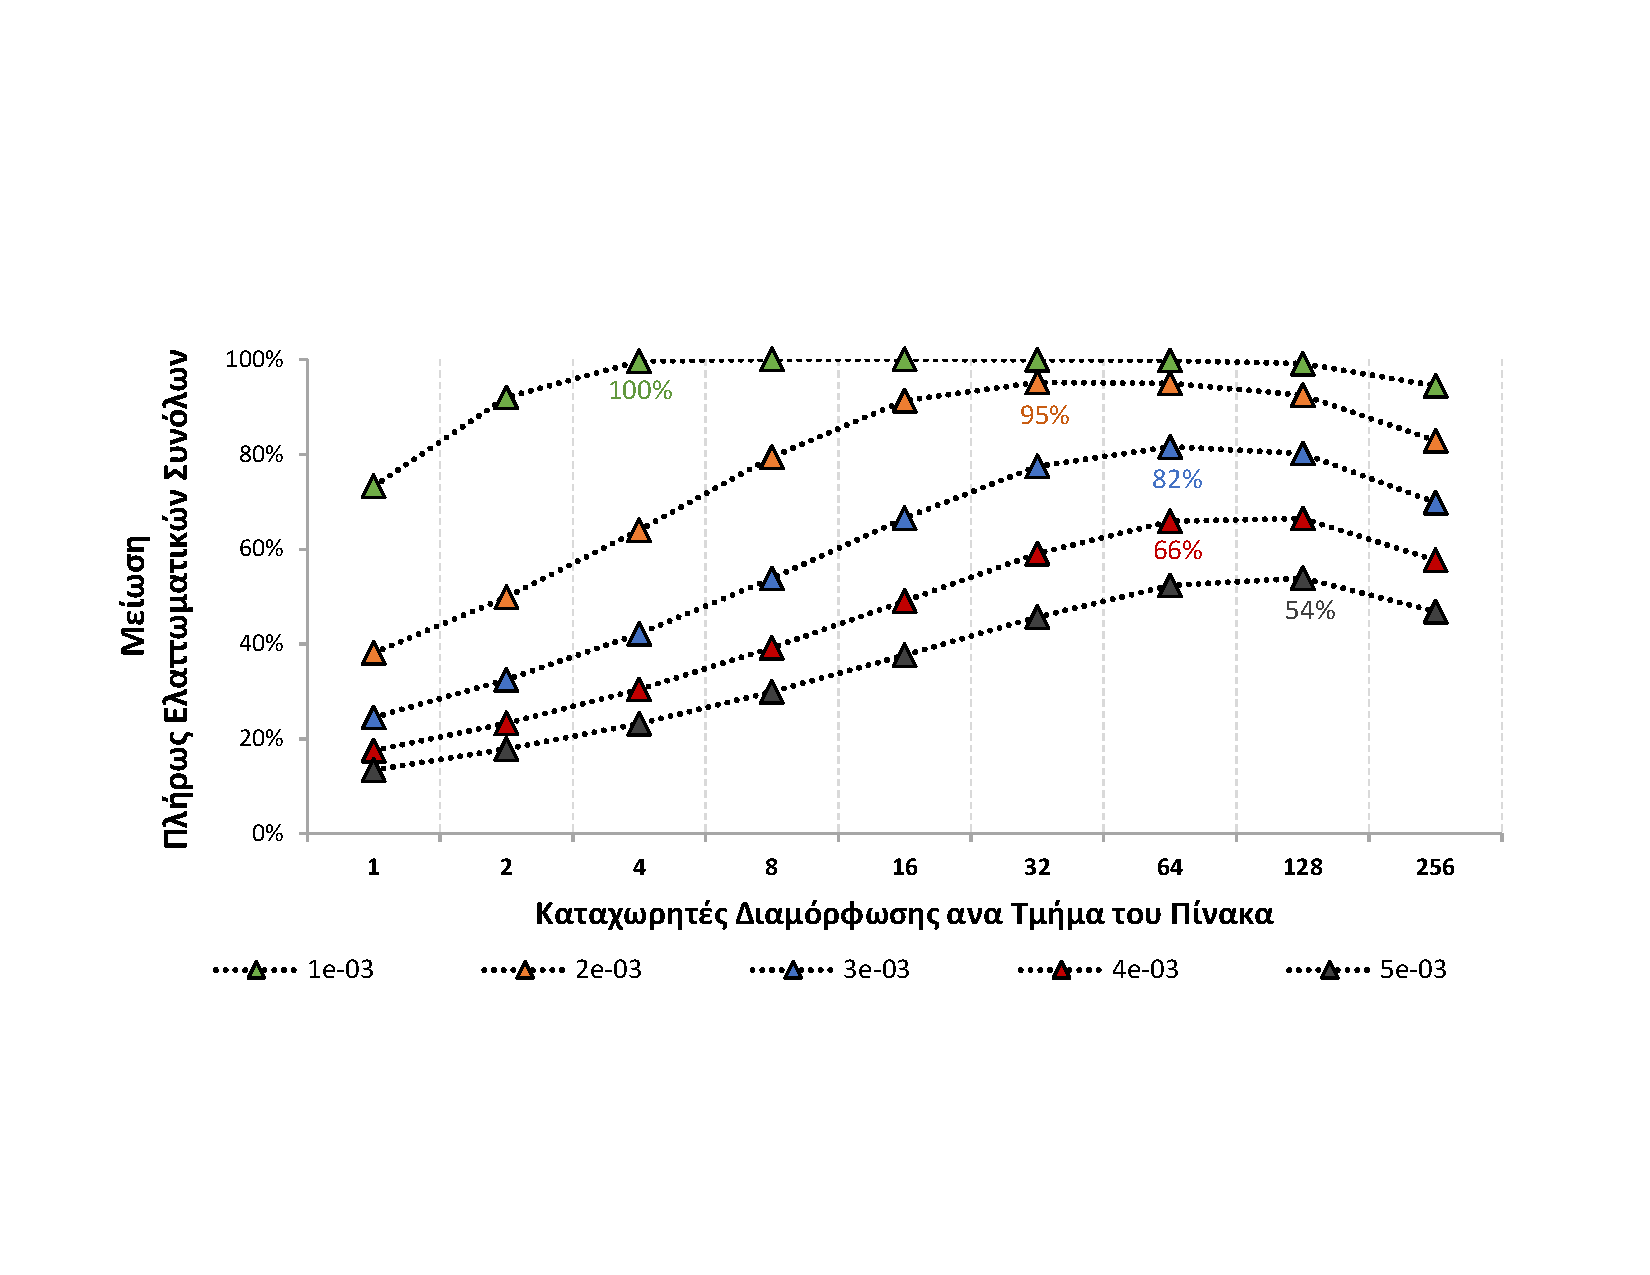
\includegraphics[width=0.99\linewidth, trim=1.9cm 5cm 1.8cm 5.9cm, clip=true]{\resultsDIR/chap5_BTB_ffsets_reduction_2048_2way.pdf}}
        \caption{ΠΠΠΔ 2048-πλαισίων / 2-τρόπων συνόλου συσχέτισης}
        \label{fig:chap5_btb_ffsets_2048_2way}
    \end{subfigure}
    
    \begin{subfigure}[t]{\textwidth}
        \centering
        \fbox{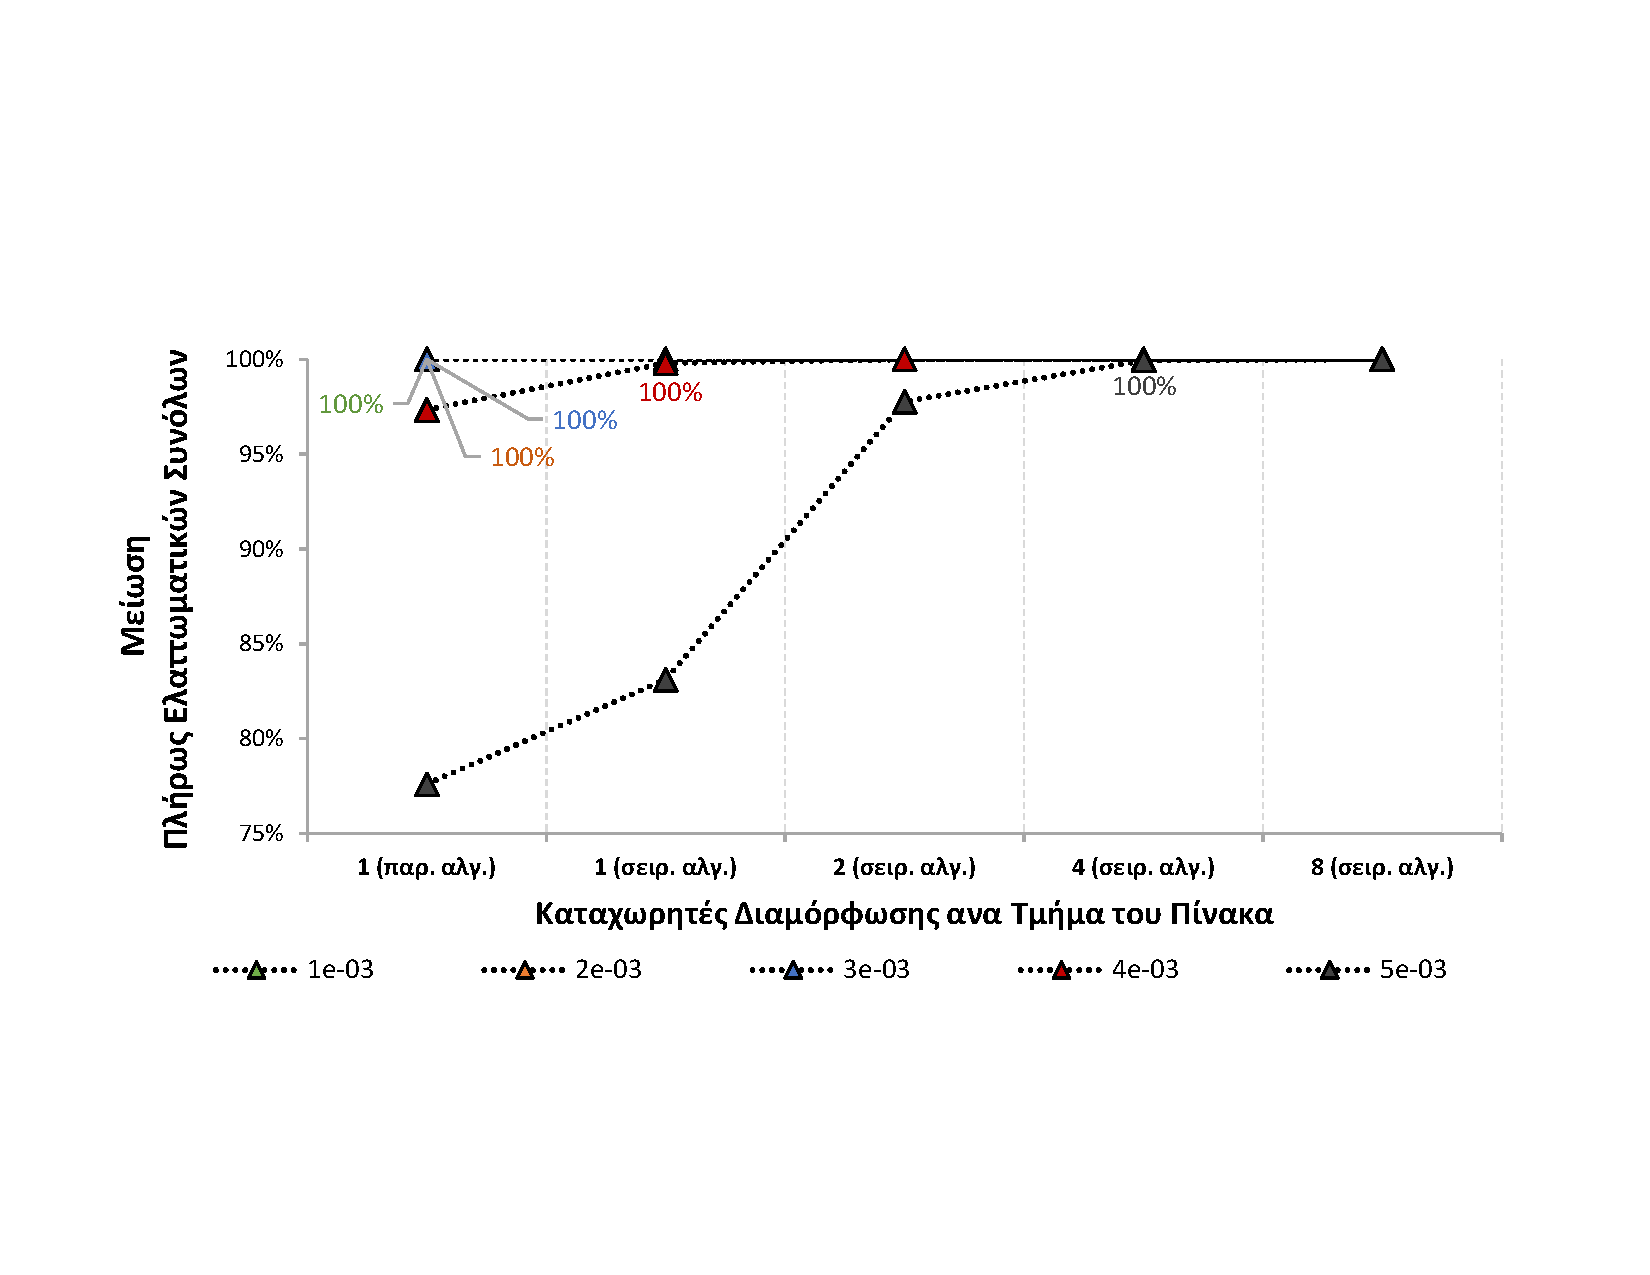
\includegraphics[width=0.99\linewidth, trim=1.9cm 5cm 1.8cm 5.9cm, clip=true]{\resultsDIR/chap5_BTB_ffsets_reduction_2048_4way.pdf}}
        \caption{ΠΠΠΔ 2048-πλαισίων / 4-τρόπων συνόλου συσχέτισης}
        \label{fig:chap5_btb_ffsets_2048_4way}
    \end{subfigure}
    \caption{Μείωση των πλήρως ελαττωματικών πλαισίων με τη χρήση παραλλαγών της μεθόδου, σε σχέση με τη μη εφαρμογή τεχνικής για τη μείωσή τους}
    \label{fig:chap5_btb_ffsets_2048}
\end{figure}

Στο Σχήμα \ref{fig:chap5_btb_ffsets_2048_4way} παρουσιάζονται τα αντίστοιχα αποτελέσματα για τον πίνακα 2048-πλαισίων/4-τρόπων. Ομοίως με το πρώτο γράφημα, κάθε σημείο του οριζόντιου άξονα αντιστοιχεί στη χρήση ενός πλήθους καταχωρητών ανά τμήμα. Συγκεκριμένα, το πρώτο και το δεύτερο σημείο κάθε καμπύλης εκφράζει τα αποτελέσματα της περίπτωσης όπου χρησιμοποιείται ένας καταχωρητής ανά τμήμα και ο υπολογισμός κατάλληλων τιμών γίνεται με τη χρήση του παράλληλου και του σειριακού αλγορίθμου αντίστοιχα.
\par
Όπως φανερώνει και το γράφημα, σε σχετικά μικρές πιθανότητες σφάλματος ($\expnum{1}$, $\expnum{2}$ και $\expnum{3}$) και οι δύο εκδοχές πετυχαίνουν την ολοκληρωτική εξάλειψη των πλήρως ελαττωματικών συνόλων. Αντιθέτων, όταν η πιθανότητα σφάλματος αυξάνεται σε $\expnum{4}$ και $\expnum{5}$ ο σειριακός αλγόριθμος παρουσιάζει αποδοτικότερα αποτελέσματα απ' ότι ο παράλληλος. Συγκεκριμένα, στην πιθανότητα σφάλματος $\expnum{4}$ ο σειριακός αλγόριθμος με χρήση ενός και μόνο καταχωρητή ανά τμήμα είναι σε θέση να εξαλείψει τα πλήρως ελαττωματικά σύνολα, ενώ στην πιθανότητα $\expnum{5}$ πετυχαίνει ποσοστό μείωσης 83\% από 78\% που πετυχαίνει ο παράλληλος. Η διαφορά αυτή οφείλεται στο γεγονός πως τα παράλληλα βήματα του αλγορίθμου εκτελούνται ανεξάρτητα. Για το λόγο αυτό, ο παράλληλος αλγόριθμος αποτελεί πειραματικό αντικείμενο και δεν συνιστάται η χρήση του όταν η μελετώμενη πιθανότητα σφάλματος είναι αυξημένη. Για την ολοκληρωτική εξάλειψης των πλήρως ελαττωματικών συνόλων στην περίπτωση της πιθανότητας σφάλματος $\expnum{4}$ απαιτείται η χρήση τουλάχιστον 4 καταχωρητών ανά τμήμα, όπως φαίνεται και από τους δείκτες γκρι αποχρώσεων του Σχήματος \ref{fig:chap5_btb_ffsets_2048_4way}.
\par
Μία πολύ σημαντική παρατήρηση που εξήχθη από τη μελέτη 1000 χαρτών σφαλμάτων για διαφορετικά μεγέθη του Πίνακα Πρόβλεψης Προορισμού Διακλάδωσης (ΠΠΠΔ) είναι η συσχέτιση του αριθμού Καταχωρητών Διαμόρφωσης που χρησιμοποιούνται με το πλήθος συνόλων που ανήκουν σε κάθε υποτμήματος. Τα γραφήματα του Σχήματος \ref{fig:chap5_btb_ffsets} παρουσιάζουν τη μείωση του αριθμού των πλήρως ελαττωματικών συνόλων σε σχέση με τη μή χρήση κάποια τεχνική, για διαφορετικές διασπάσεις των τμημάτων σε υποτμήματα, δηλαδή διαφορετικά πλήθη συνόλων ανά καταχωρητή διαμόρφωσης. Η μελέτη πραγματοποιήθηκε για μνήμες 512, 1024, 2048 και 4096 πλαισίων.
\par
Στο γράφημα του Σχήματος \ref{fig:chap5_btb_ffsets_2way} που αναφέρεται στην περίπτωση οργάνωσης 2-τρόπων συνόλου συσχέτισης, παρατηρούμε πως για τις πιθανότητες σφάλματος $\expnum{1}$, $\expnum{2}$, $\expnum{3}$, $\expnum{4}$ και $\expnum{5}$ οι κατάλληλες επιλογές συνόλων ανά καταχωρητή είναι 256, 32, 16, 8 και 8 αντίστοιχα. Η μείωση των πλήρως ελαττωματικών συνόλων σε αυτές τις περιπτώσεις θα είναι 100\%, 95\%, 82\%, 67\% και 54\% ανεξαρτήτως μεγέθους. Επομένως, τα βέλτιστα αποτελέσματα που επισημάνθηκαν στην περίπτωση του πίνακα 2048-πλαισίων του Σχήματος \ref{fig:chap5_btb_ffsets_2048_2way} αντιστοιχούν σε αυτές τις βέλτιστες διασπάσεις των συνόλων. Όπως και στην περίπτωση του πίνακα 2048-πλαισίων/2-τρόπων, η μεγάλη διάσπαση των συνόλων μπορεί να επιφέρει αρνητικά αποτελέσματα όπως φαίνεται και από τα τελευταία σημεία των καμπυλών του Σχήματος \ref{fig:chap5_btb_ffsets_2way}.
\par
Το γράφημα του Σχήματος \ref{fig:chap5_btb_ffsets_4way} αναφέρεται στην αντίστοιχη μελέτη μνημών οργάνωσης 4-τρόπων συνόλου συσχέτισης. Αριθμώντας τα σημεία των καμπυλών από αριστερά προς τα δεξιά, τα μονά σημεία αντιστοιχούν στα αποτελέσματα όταν χρησιμοποιείται ο παράλληλος αλγόριθμος για τον υπολογισμό κατάλληλων τιμών, ενώ τα ζυγά στα αποτελέσματα όταν χρησιμοποιείται ο σειριακός. Όπως και στην περίπτωση του πίνακα 2048-πλαισίων του Σχήματος \ref{fig:chap5_btb_ffsets_2048_4way}, στις  πιθανότητες σφάλματος $\expnum{1}$, $\expnum{2}$ και $\expnum{3}$ είναι δυνατή η επίτευξη ολοκληρωτικής εξάλειψης των πλήρως ελαττωματικών συνόλων. Αντιθέτως, όταν οι πιθανότητα σφάλματος αυξάνεται σε $\expnum{4}$ και $\expnum{5}$, για να επιτευχθεί η ολοκληρωτική τους εξάλειψη πρέπει τα σύνολα να διασπαστούν σε τμήματα των 128 συνόλων το κάθε ένα.

\begin{figure}[!t]
    \centering
    \begin{subfigure}[t]{\textwidth}
        \centering
        \fbox{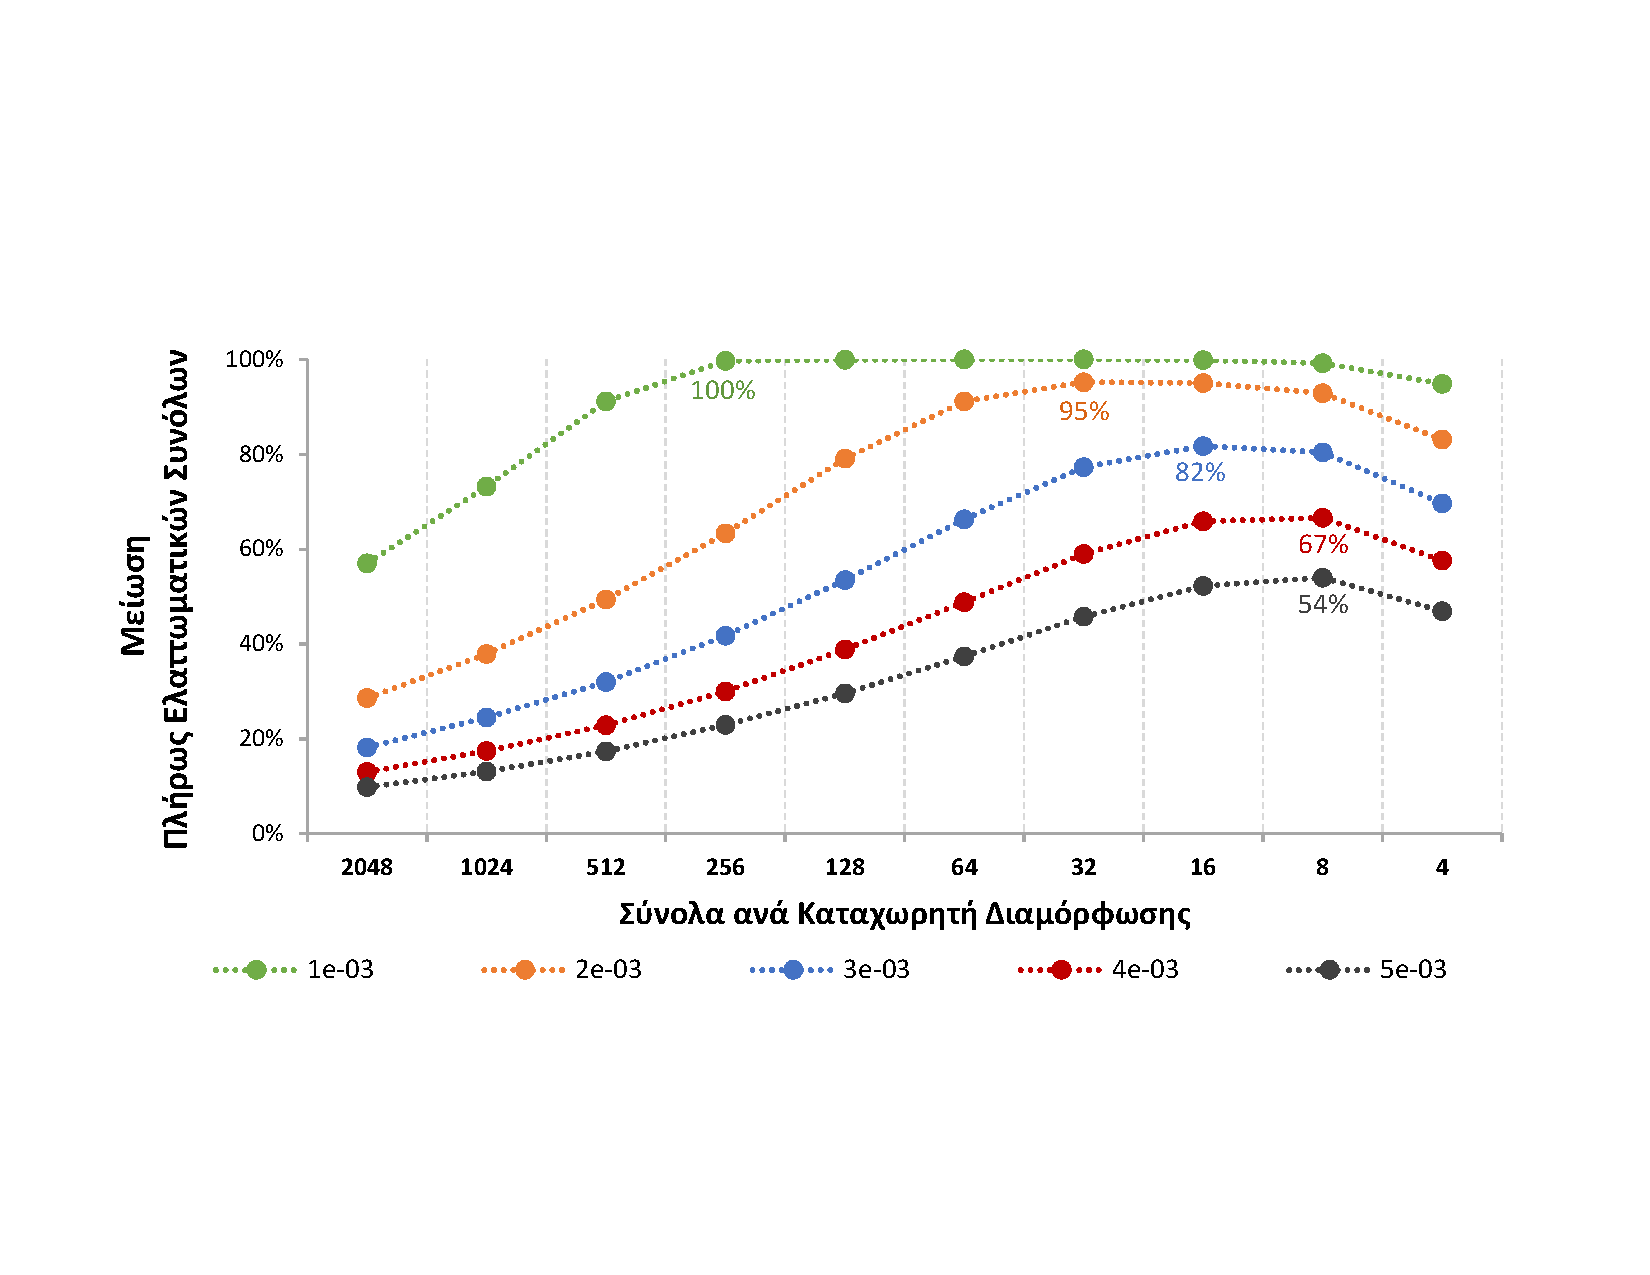
\includegraphics[width=0.99\linewidth, trim=1.9cm 5cm 1.8cm 5.9cm, clip=true]{\resultsDIR/chap5_BTB_ffsets_reduction_2way.pdf}}
        \caption{ΠΠΠΔ 2-τρόπων συνόλου συσχέτισης}
        \label{fig:chap5_btb_ffsets_2way}
    \end{subfigure}
    
    \begin{subfigure}[t]{\textwidth}
        \centering
        \fbox{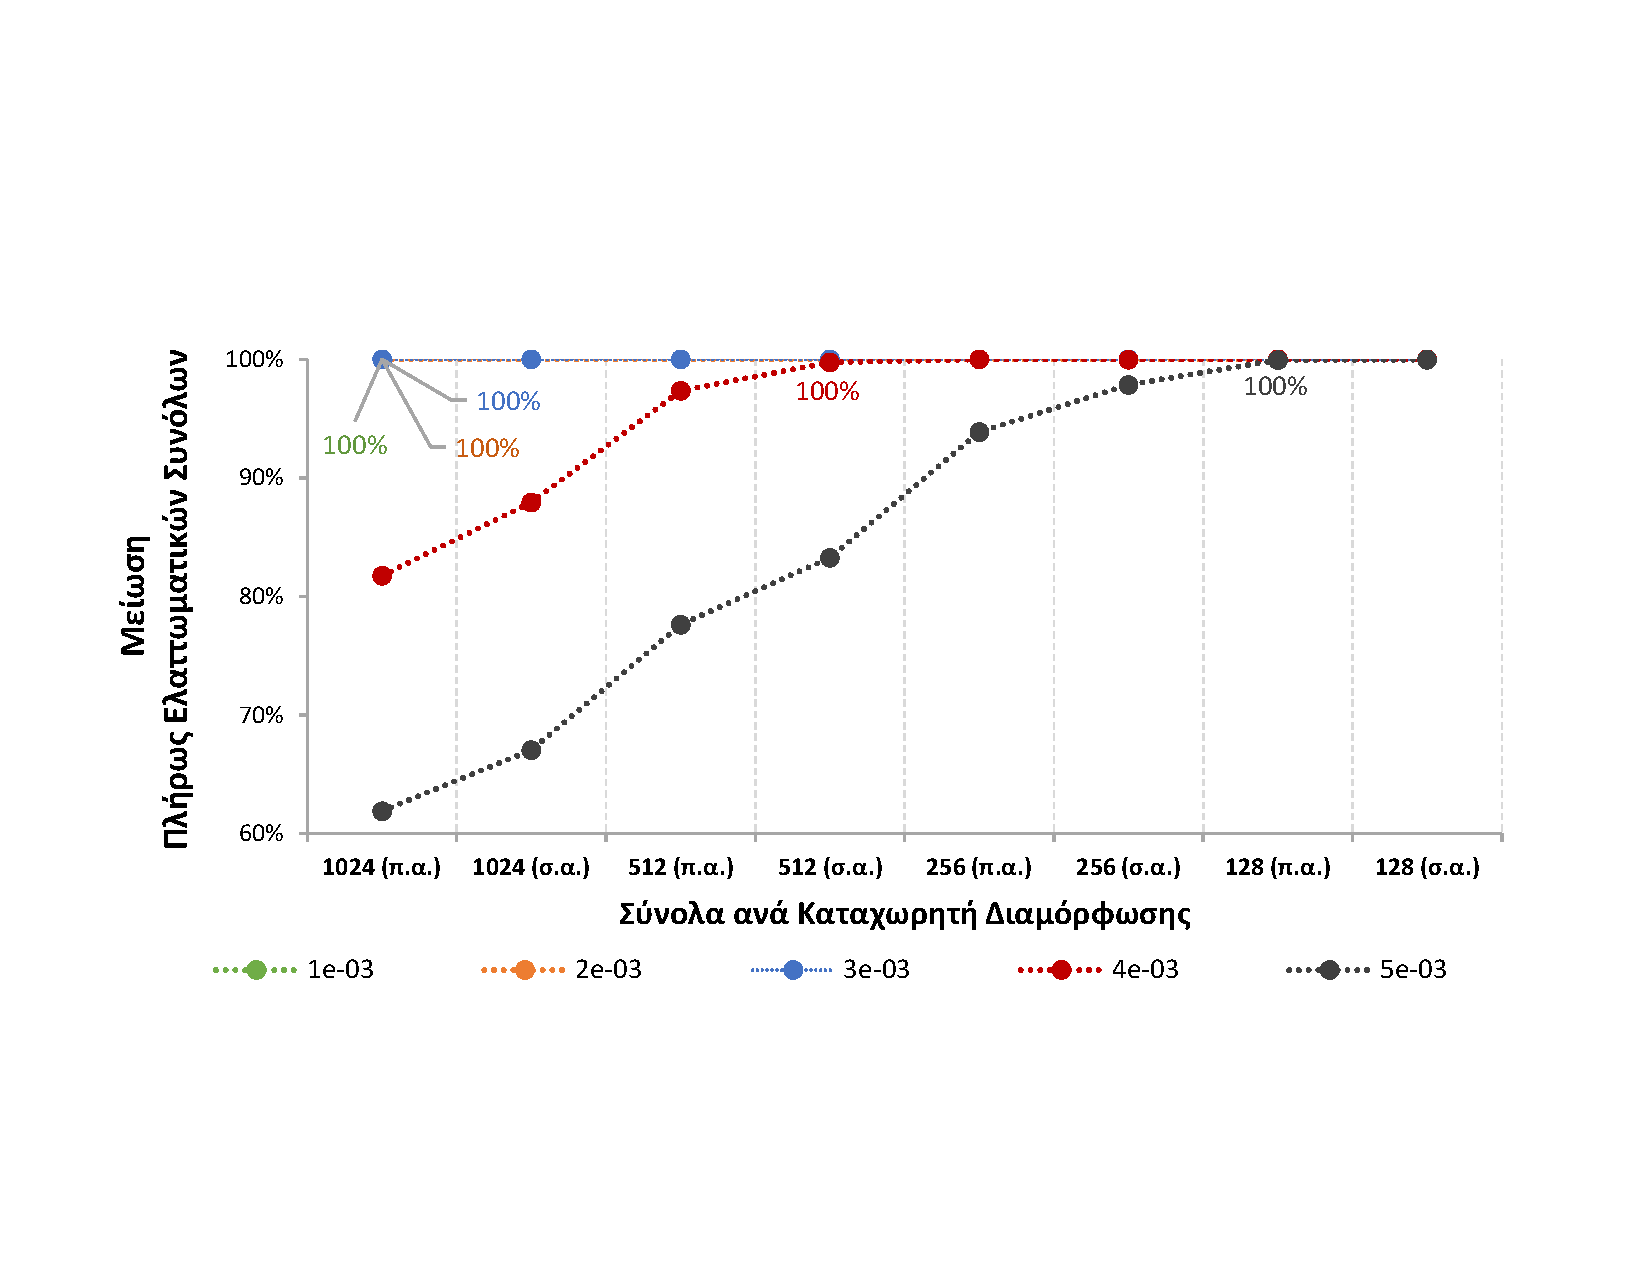
\includegraphics[width=0.99\linewidth, trim=1.9cm 5cm 1.8cm 5.9cm, clip=true]{\resultsDIR/chap5_BTB_ffsets_reduction_4way.pdf}}
        \caption{ΠΠΠΔ 4-τρόπων συνόλου συσχέτισης}
        \label{fig:chap5_btb_ffsets_4way}
    \end{subfigure}
    \caption{Μείωση των πλήρως ελαττωματικών πλαισίων με τη χρήση παραλλαγών της μεθόδου σε σχέση με τη μη εφαρμογή τους}
    \label{fig:chap5_btb_ffsets}
\end{figure}

%----------------------------------------------------------%

\section{Προσέγγιση Χειρότερης Περίπτωσης}
\label{chap5_maxFFSets_num}

Μελετώντας προσεκτικά τον αλγόριθμο εξάγεται ένα πολύ σημαντικό συμπέρασμα, η δυνατότητα εύρεσης του μέγιστου αριθμού πλήρως ελαττωματικών συνόλων που μπορεί να προκύψουν μετά την εφαρμογή της τεχνικής. Η μόνη γνώση που απαιτείται είναι το πλήθος ελαττωματικών πλαισίων ανά τμήμα. Το δεδομένο αυτό αποτελεί μία εκτίμηση του αποτελέσματος του αλγορίθμου, για την χειρότερη περίπτωση κατανομής των ελαττωματικών πλαισίων.
\par
Έστω ότι $f_1$ και $f_2$ το πλήθος των σφαλμάτων στα δύο τμήματα ενός Πίνακας Πρόβλεψης Προορισμού Διακλάδωσης 2-τρόπων, με $S$ σύνολα συσχέτισης. Στην χειρότερη περίπτωση αρχικής κατανομής των σφαλμάτων, η εφαρμογής της πρώτης μεθόδου θα περιόριζε τα πλήρως ελαττωματικά σύνολα σε:

\begin{equation}
    \label{eqn:chap5_maxFFSETS_2way}
    X = \floor*{ \frac{f_1 \times f_2}{S} }
\end{equation}

Η εξίσωση αυτή προέρχεται από το γεγονός ότι οι πράξεις \xor που πραγματοποιούνται μεταξύ των δύο τμημάτων, θα είναι όσο και το γινόμενο του πλήθους ελαττωματικών πλαισίων τους ($f_1 \times f_2$), όπως αναφέρθηκε και στην ανάλυση των παραδειγμάτων. Η σχέση \ref{eqn:chap5_maxFFSETS_2way} μπορεί να γίνει κατανοητή από ένα παράδειγμα όπου για κάθε εκτέλεση μίας πράξης \xor ενημερώνεται διαφορετικός μετρητής, ώστε οι μετρητές να αυξάνονται ομοιόμορφα τελικά (για παράδειγμα: $XFB=000 \rightarrow XFB=001 \rightarrow XFB=010 \rightarrow ... \rightarrow XFB=111 \rightarrow XFB=000 \rightarrow XFB=001 \rightarrow ... $). Συνεπώς, εάν όλα τα πλαίσια είναι ελαττωματικά τότε κάθε μετρητής θα έχει την τιμή $S$. Στην περίπτωσης ομοιόμορφης αύξησης η επιλογή κατάλληλης τιμής γίνεται δυσκολότερη, σε αντίθεση με την περίπτωση όπου ένα αποτέλεσμα επαναλαμβάνεται περισσότερες φορές, και επομένως ο αντίστοιχος μετρητής-α αυξάνεται περισσότερες φορές σε σχέση με ένα μετρητή-β (το σύνολο των αυξήσεων παραμένει σταθερό). Έτσι η τιμή που αντιστοιχεί στον μετρητή-β είναι η επιθυμητή.
\par
Μέσω της εξίσωσης \ref{eqn:chap5_maxFFSETS_2way} μπορεί να γίνει μία εκτίμηση της χειρότερης περίπτωσης προτού γίνει η εκτέλεση του αλγορίθμου. Η στρογγυλοποίηση του αριθμού προς τον πλησιέστερο μικρότερο ακέραιο αριθμό (\en{floor}) γίνεται διότι το πλήθος των πλήρως ελαττωματικών συνόλων είναι ακέραιος αριθμός.
\par
Για την περίπτωση ενός Πίνακας Πρόβλεψης Προορισμού Διακλάδωσης 4-τρόπων με πλήθος σφαλμάτων ανά τμήμα $f_1, f_2, f_3$ και $f_4$ αντίστοιχα, το όριο αυτό υπολογίζεται ως:

\begin{equation}
    \label{eqn:chap5_maxFFSETS_X}
    X = \floor*{ \frac{ \floor*{ \frac{ \floor*{ \frac{f_1 \times f_2}{S} } \times f_3}{S} } \times f_4}{S} }
\end{equation}

\noindent όπου $f_i$ είναι το πλήθος ελαττωματικών πλαισίων του Τμήματος-$i$ και $S$ ο αριθμός συνόλων του Πίνακας Πρόβλεψης Προορισμού Διακλάδωση, όπως προαναφέρθηκε.
\par
Η σχέση \ref{eqn:chap5_maxFFSETS_X} συνεπάγεται από το ότι ο αλγόριθμος εκτελείται σειριακά και για κάθε βήμα του χρησιμοποιούνται οι άλυτες περιπτώσεις του προηγούμενου βήματος. Επομένως, για τον υπολογισμό της χειρότερης περίπτωσης, αρκεί να γίνει η υπόθεση πως σε κάθε βήμα χρησιμοποιείται η χειρότερη περίπτωση αποτελέσματος του προηγούμενου βήματος.

%----------------------------------------------------------%

\section{Υλοποίηση της Τεχνικής στο Υλικό}
\label{chap5_HardwareImplementation}

Η υλοποίηση της τεχνικής απαιτεί ελάχιστη αύξηση του υλικού. Για παράδειγμα σε ένα πίνακα 2048-πλαισίων/2-τρόπων στον οποίο χρησιμοποιούνται 64 καταχωρητές ανά τμήμα, τα στοιχεία που απαιτούνται είναι 128 καταχωρητές των 4 δυαδικών ψηφίων για την αποθήκευση πληροφορίας (512 κυψελίδες συνολικά), καθώς και 512 πύλες \xor ενός επιπέδου. Επομένως, η αύξηση θα είναι μικρότερη από 1\% . Αυτό αποτελεί πολύ σημαντικό γεγονός εάν συγκριθεί η συγκεκριμένη τεχνική με ήδη υπάρχουσες τεχνικές για Κρυφές Μνήμες Δεδομένων και Εντολών, όπως για παράδειγμα η \cite{shirvani1999padded} με την οποία θα ήταν δυνατή η πλήρης εξάλειψη των πλήρως ελαττωματικών συνόλων μέσω της ανακατεύθυνσης των ελαττωματικών πλαισίων σε υγιή, όμως με μία αύξηση του υλικού μεγαλύτερη του 20\%.
\par
Στα Σχήματα \ref{fig:chap5_permutation_impl_v1} και \ref{fig:chap5_permutation_impl_v2} όπου αναδεικνύεται η υλοποίηση της τεχνικής, παρουσιάζονται δύο διαφορετικές εκδοχές, ώστε να αφήνεται στο σχεδιαστή η απόφαση του τρόπου υλοποίησης αναλόγως του κόστους κάθε μίας. Η πρώτη υλοποίηση απαιτεί τη χρησιμοποίηση πολλαπλών μικρότερων αποκωδικοποιητών, το οποίο μπορεί να επιφέρει μικρή αύξηση στην κατανάλωση και την επιφάνεια. Η δεύτερη υλοποίηση απαιτεί την προσθήκη πολυπλεκτών στο μονοπάτι της διευθυνσιοδότηση ώστε να επιλέγεται ο κατάλληλος Καταχωρητής Διαμόρφωσης. Η λύση αυτή μπορεί να επιφέρει αύξηση της απαιτούμενης επιφάνειας και πιθανώς μικρή καθυστέρηση στην εξαγωγή δεδομένου από τον Πίνακα Πρόβλεψης Προορισμού Διακλάδωσης. Τέλος, θα μπορούσε να γίνει ενσωμάτωση μίας υβριδικής υλοποίησης όπου χρησιμοποιούνται λιγότεροι πολυπλέκτες σε συνδυασμό με ένα μικρό πλήθος αποκωδικοποιητών. Το κόστος για κάθε υλοποίηση εξαρτάται άμεσα από την τεχνολογία που χρησιμοποιεί κάθε σχεδιαστής.

\begin{figure}[h]
    \centering
    \fbox{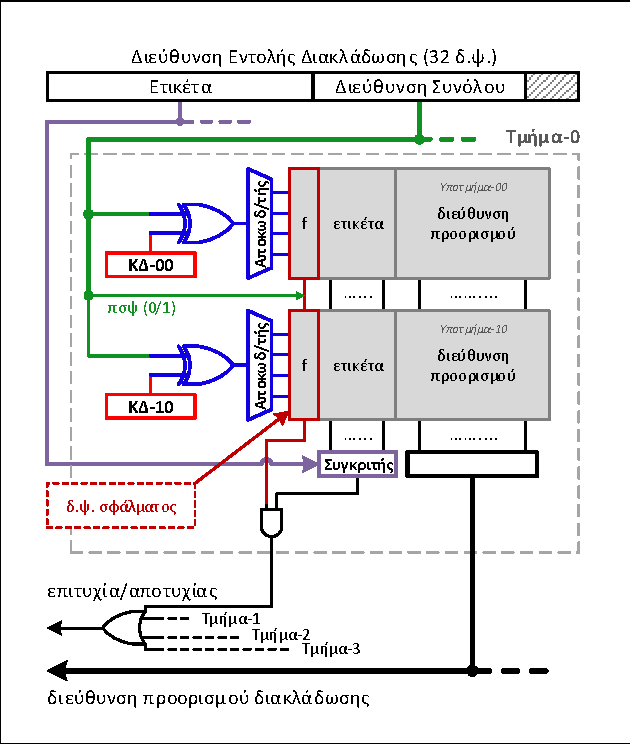
\includegraphics[width=0.8\linewidth,trim=0.5cm 0.6cm 0.5cm 0.8cm, clip=true]{\hardwareDIR/chap5_high_level_diagram_v1.pdf}}
    \caption{1\textsuperscript{ος} Τρόπος Υλοποίησης - Διάσπαση αποκωδικοποιητή}
    \label{fig:chap5_permutation_impl_v1}
\end{figure}

\begin{figure}[t]
    \centering
    \fbox{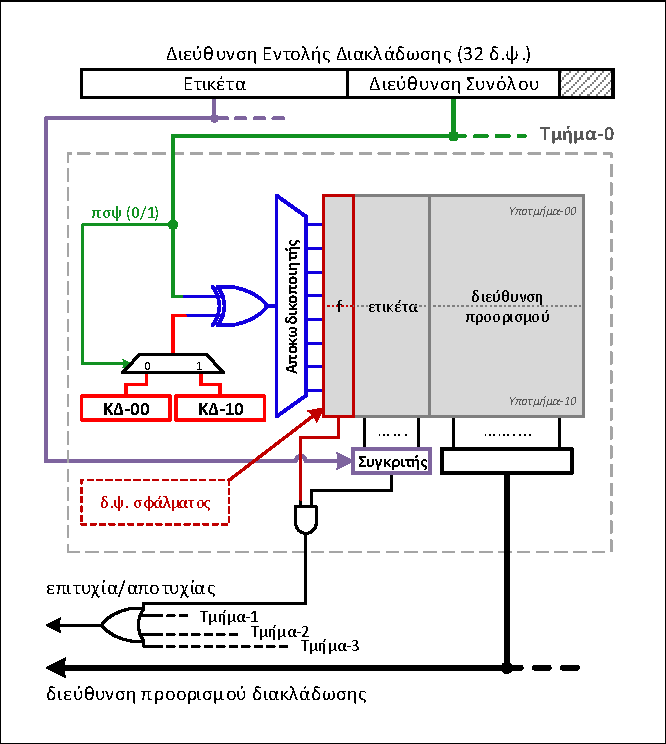
\includegraphics[width=0.8\linewidth,trim=0.5cm 0.6cm 0.5cm 0.6cm, clip=true]{\hardwareDIR/chap5_high_level_diagram_v2.pdf}}
    \caption{2\textsuperscript{ος} Τρόπος Υλοποίησης - Προσθήκη πολυπλέκτη}
    \label{fig:chap5_permutation_impl_v2}
\end{figure}

Παρά το γεγονός πως η διάσπαση σε υποτμήματα συνεπάγεται και μερική αύξηση της κατανάλωσης του Πίνακα Πρόβλεψης Προορισμού Διακλάδωσης, η μείωση του χρόνου ολοκλήρωσης ενός προγράμματος εξαιτίας της μεγάλης μείωσης των πλήρως ελαττωματικών συνόλων θα οδηγήσει τελικώς σε σημαντική μείωση της συνολικής κατανάλωσης του ολοκληρωμένου κυκλώματος. Τα αποτελέσματα τόσο της μείωσης της κατανάλωσης όσο και της απώλειας που υφίσταται η απόδοση του υπερβαθμωτού επεξεργαστή παρουσιάζονται στο Κεφάλαιο \ref{chap6}.


%----------------------------------------------------------%

    \chapter{Πειραματική Αξιολόγηση}
\label{chap6}

\section{Εισαγωγή}
\label{chap6_Intro}

Για την αξιολόγηση της προτεινόμενης τεχνικής αντιμετώπισης των πλήρως ελαττωματικών συνόλων του Πίνακα Πρόβλεψης Προορισμού Διακλάδωσης εκτελέστηκαν εξομοιώσεις για 100 διαφορετικούς χάρτες σφαλμάτων και για όλα τα μετροπρογράμματα της σουίτας \spec. Επιπλέον, για κάθε περίπτωση χάρτη σφαλμάτων εκτελέστηκαν εξομοιώσεις για τρεις διαφορετικές παραλλαγές της τεχνικής. Στο παρόν κεφάλαιο παρουσιάζεται ο μέσος όρος των αποτελεσμάτων τους. Στο πρώτο τμήμα του κεφαλαίου μελετάται η βελτίωση της απόδοσης του υπερβαθμωτού επεξεργαστή όταν ενσωματώνεται η τεχνική της λογικής μετάθεσης πλαισίων στον Πίνακα Πρόβλεψης Προορισμού Διακλάδωσης. Στο δεύτερο τμήμα παρουσιάζονται τα αντίστοιχα αποτελέσματα ενέργειας ώστε να αποκαλυφθεί εάν η χρήση της προτεινόμενης τεχνικής επιφέρει ή όχι τη συνολική μείωση της κατανάλωσης του συστήματος.

%----------------------------------------------------------%

\section{Παράμετροι Αξιολόγησης}
\label{chap6_EvaluationParameters}

Η μελέτη που ακολουθεί επικεντρώνεται σε μνήμες των 2048 πλαισίων και δύο διαφορετικών μεγεθών οργάνωσης συνόλου συσχέτισης (τμήματα). Οι διαμορφώσεις αυτές αποτελούν μία μέση περίπτωση των σύγχρονων εμπορικών επεξεργαστών και για το λόγο αυτό μπορούν να θεωρηθούν αντικειμενικές. Όπως αναφέρθηκε και στην Ενότητα \ref{chap4_BTBConfigIPC}, ένας Πίνακας Πρόβλεψης Προορισμού Διακλάδωσης (ΠΠΠΔ) των 2048 πλαισίων έχει τη δυνατότητα να προσφέρει την απόδοση ακόμη και μίας εξαιρετικά μεγάλης μνήμης των 16384 πλαισίων.
\par
Για κάθε περίπτωση λειτουργίας χαμηλού δυναμικού εξετάζεται η μεταβολή της απόδοσης και της καταναλισκόμενης ενέργειας εξαιτίας της ύπαρξης ελαττωματικών κυψελίδων στον Πίνακα Πρόβλεψης Προορισμού Διακλάδωσης. Συγκεκριμένα μελετώνται οι δύο περιπτώσεις δυναμικού που αντιστοιχούν στις πιθανότητες σφάλματος $\expnum{2}$ (πιθανότητα-1) και $\expnum{5}$ (πιθανότητα-2).
\par
Σε κάθε περίπτωση εξομοιώθηκαν τέσσερα είδη μοντέλων Πίνακα Πρόβλεψης Προορισμού Διακλάδωσης. Το σύνολο των εξομοιώσεων που πραγματοποιήθηκαν για κάθε χάρτη σφαλμάτων και μετροπρόγραμμα παρουσιάζονται στον Πίνακα \ref{tab:chap6_LowPowerSimulations}.

\begin{table}[t]
    \centering
    \begin{tabularx}{\textwidth}{!{\vrule width 4\arrayrulewidth} >{\centering\arraybackslash}X | >{\centering\arraybackslash}X | >{\centering\arraybackslash}X !{\vrule width 4\arrayrulewidth}}
        \Xhline{4\arrayrulewidth}
        \textbf{Μοντέλο ΠΠΠΔ}   & \textbf{Οργάνωση ΠΠΠΔ}                 & \textbf{Πιθανότητα Σφάλματος (Συχνότητα)} \\
        \Xhline{4\arrayrulewidth}
        
        \multirow{4}{*}{Βασικό} & \multirow{2}{*}{2048-πλαίσια/2-τρόπων} & {$\expnum{2}\ (1.1GHz)$} \\ \cline{3-3}
                                &                                        & {$\expnum{5}\ (0.5GHz)$} \\ \cline{2-3}
                                & \multirow{2}{*}{2048-πλαίσια/4-τρόπων} & {$\expnum{2}\ (1.1GHz)$} \\ \cline{3-3}
                                &                                        & {$\expnum{5}\ (0.5GHz)$} \\
        \hline
        
        \multirow{4}{\linewidth}{\centering Ενισχυμένο Σειριακό} & \multirow{2}{*}{2048-πλαίσια/2-τρόπων} & {$\expnum{2}\ (1.1GHz)$} \\ \cline{3-3}
                                                                 &                                        & {$\expnum{5}\ (0.5GHz)$} \\ \cline{2-3}
                                                                 & \multirow{2}{*}{2048-πλαίσια/4-τρόπων} & {$\expnum{2}\ (1.1GHz)$} \\ \cline{3-3}
                                                                 &                                        & {$\expnum{5}\ (0.5GHz)$} \\
        \hline
        
        \multirow{4}{\linewidth}{\centering Ενισχυμένο Παράλληλο} & \multirow{4}{*}{2048-πλαίσια/4-τρόπων} & \multirow{2}{*}{$\expnum{2}\ (1.1GHz)$} \\
                                                                  &                                        &                          \\ \cline{3-3}
                                                                  &                                        & \multirow{2}{*}{$\expnum{5}\ (0.5GHz)$} \\
                                                                  &                                        &                          \\
        \hline
        
        \multirow{4}{\linewidth}{\centering Βελτιστοποιημένο Σειριακό} & \multirow{2}{*}{2048-πλαίσια/2-τρόπων} & {$\expnum{2}\ (1.1GHz)$} \\ \cline{3-3}
                                                                          &                                        & {$\expnum{5}\ (0.5GHz)$} \\ \cline{2-3}
                                                                          & \multirow{2}{*}{2048-πλαίσια/4-τρόπων} & {$\expnum{2}\ (1.1GHz)$} \\ \cline{3-3}
                                                                          &                                        & {$\expnum{5}\ (0.5GHz)$} \\
        \hline
        
        \hline
        \textbf{Σύνολο Εξομοιώσεων} & \multicolumn{2}{c !{\vrule width 4\arrayrulewidth}}{14 $\times$ 29 μετροπρογράμματα $\times$ 100 χάρτες σφ. = \textbf{40600}} \\
        \Xhline{4\arrayrulewidth}
    \end{tabularx}
    \caption{Εκτελούμενες εξομοιώσεις σε λειτουργία χαμηλής κατανάλωσης}
    \label{tab:chap6_LowPowerSimulations}
\end{table}

Για κάθε ένα από τα τέσσερα εξομοιούμενα μοντέλα που παρουσιάζονται στον Πίνακα \ref{tab:chap6_LowPowerSimulations} ισχύουν οι ακόλουθες παραδοχές:
\begin{description}
    \item[Βασικό:] Απενεργοποίηση όλων των ελαττωματικών πλαισίων.
    \item[Ενισχυμένο Σειριακό:] Απενεργοποίηση όλων των ελαττωματικών πλαισίων και λογική μετάθεση τους με τη χρήση ενός καταχωρητή ανά τμήμα. Η εύρεση κατάλληλων τιμών προκύπτει από την εκτέλεση του σειριακού αλγορίθμου.
    \item[Ενισχυμένο Παράλληλο:] Απενεργοποίηση όλων των ελαττωματικών πλαισίων και λογική μετάθεση τους με τη χρήση ενός καταχωρητή ανά τμήμα. Η εύρεση κατάλληλων τιμών προκύπτει από την εκτέλεση του παράλληλου αλγορίθμου.
    \item[Βελτιστοποιημένο Σειριακό:] Απενεργοποίηση όλων των ελαττωματικών πλαισίων και λογική μετάθεση τους με τη χρήση πολλαπλών καταχωρητών ανά τμήμα. Η εύρεση κατάλληλων τιμών προκύπτει από την εκτέλεση του σειριακού αλγορίθμου.
\end{description}

%----------------------------------------------------------%

\section{Σύστημα Αξιολόγησης}
\label{chap6_EvaluationSystem}

Για την αξιολόγηση της τεχνικής χρησιμοποιήθηκες ο το μαθηματικό εργαλείο \matlab για την εξαγωγή των 100 χαρτών σφαλμάτων, σε συνδυασμό με τον εγκεκριμένο εξομοιωτή αρχιτεκτονικής υπολογιστών \gem. Επιπλέον, χρησιμοποιήθηκε το εργαλείο υπολογισμού κατανάλωσης \mcpat το οποίο δέχεται ως είσοδο τα αποτελέσματα της εξομοίωσης. Για τον υπολογισμό της ισχύος του Πίνακα Πρόβλεψης Προορισμού Διακλάδωσης και αξιοποιεί το εργαλείο \cacti, το οποίο ενσωματώνεται στον πηγαίο του κώδικα. Αναλυτικές πληροφορίες για τα τρία αυτά εργαλεία βρίσκονται στα \cite{release2013mathworks}, \cite{binkert2011gem5} και \cite{li2009mcpat, muralimanohar2009cacti} αντίστοιχα. Στο Κεφάλαιο \ref{chap7} γίνεται λεπτομερής περιγραφή της διαδικασία αξιολόγησης και του τρόπου χρήσης των εργαλείων.
\par
Στον Πίνακα \ref{tab:chap6_gem5parameters} παρουσιάζονται οι λεπτομέρειες του εξομοιούμενου \en{x86} επεξεργαστή που χρησιμοποιήθηκε κατά την εκτέλεση των πειραμάτων, καθώς και επιπλέον πληροφορίες για τα μετροπρογράμματα που χρησιμοποιήθηκαν.

\begin{otherlanguage}{english}
    \begin{table}[h]
        \centering
        \begin{tabularx}{\textwidth}{ >{\centering\arraybackslash}X || >{\centering\arraybackslash}X }
            
            \Xhline{4\arrayrulewidth}
            
            \textbf{\gr{Παράμετροι}}                                        & \textbf{\gr{Τιμές}}                \\
            
            \Xhline{4\arrayrulewidth}
            
            CPU Architecture / ISA                                          & Out of Order / x86                 \\ \hline
            
            ROB/IQ/LQ/SQ/Registers                                          & 256/128/128/128/256                \\ \hline
            
            Pipeline Depth                                                  & 10                                 \\ \hline
            
            Fetch/Issue/Commit Width                                        & 8/8/8 Instructions Per Cycle       \\ \hline
            
            {}                                                              & Local History Table: 4k-entries,   \\
            Combined Branch Predictor                                       & Local Predictor: 4k-entries,       \\
            (Tournament Predictor)                                          & Global Predictor: 16k-entries,     \\
            {}                                                              & Choice Predictor: 16k-entries      \\ \hline
            
            Branch Target Buffer                                            & 2048-entries, 2-way/4-way          \\ \hline
            
            \multirow{2}{*}{L1 Instruction \& L1 Data Caches}               & 64kB, 8-way, 64B-block, 1-cycle,   \\
                                                                            & LRU, MSHRS, Write Buffers          \\ \hline
                                                                
            \multirow{2}{*}{L2 Cache}                                       & 8MB, 32-way, 64B-block, 15-cycles, \\
                                                                            & LRU, 40 MSHRS, Write Buffers       \\ \hline
            
            Stride Prefetcher (L2 Cache)                                    & PC-indexed, 128-entries 8-degree   \\ \hline
            
            DRAM                                                            & 2GB, 60ns, 12.8GB/s                \\ \hline
            
            Process Technology                                              & 22nm SOI                           \\ \hline
            
            Nominal Operation                                               & 2.5GHz, 1Volt                      \\ \hline
            
            Studied SRAM                                                    & pfail1: 2e-03 (1.1GHz, 0.47Volts)  \\ \cline{2-2}
            Probabilities of Failures (pfails) \cite{lorente2014analyzing}  & pfail2: 5e-03 (0.5GHz, 0.42Volts)  \\ \hline
            
            \multirow{2}{*}{\spec Benchmarks \cite{henning2006spec}}        & 17 Floating Point (SPECfp2006)     \\
                                                                            & 12 Integer (SPECint2006)           \\ \hline
            
            Simulated Instructions                                          & 3B Warm-up, 500M Committed         \\ \hline
            
            \Xhline{4\arrayrulewidth}
        \end{tabularx}
        \caption{\gr{Παράμετροι εξομοιωτή} \gem}
        \label{tab:chap6_gem5parameters}
    \end{table}
\end{otherlanguage}

%----------------------------------------------------------%

\section{Αποτελέσματα \gem}
\label{chap6_gem5Results}

Στην παρούσα ενότητα αναδεικνύεται η βελτίωση που προσφέρει η μελετώμενη τεχνική (ενισχυμένο/βελτιστοποιημένο μοντέλο) στο χρόνο εκτέλεσης ενός προγράμματος (Εντολές ανά Κύκλο Ρολογιού - \ipc), συγκριτικά με την απλή απενεργοποίηση των ελαττωματικών πλαισίων (βασικό μοντέλο). Στην πρώτη υποενότητα μελετάται η περίπτωση όπου κάθε τμήμα του Πίνακα Πρόβλεψης Προορισμού Διακλάδωσης (ΠΠΠΔ) περιέχει έναν καταχωρητή διαμόρφωσης και για τον υπολογισμό τιμών χρησιμοποιείται ο σειριακός αλγόριθμος. Στη δεύτερη υποενότητα μελετάται η περίπτωση όπου ο υπολογισμός τιμών των καταχωρητών γίνεται μέσω του παράλληλου αλγορίθμου. Στη τρίτη και τελευταία υποενότητα μελετάται η περίπτωσης όπου τα τμήματα του Πίνακα Πρόβλεψης Προορισμού Διακλάδωσης χωρίζονται σε υποτμήματα με ένα ξεχωριστό Καταχωρητή Διαμόρφωσης για κάθε ένα, οι τιμές των οποίων υπολογίζονται μέσω του σειριακού αλγορίθμου.
\par
Για την περίπτωση του βελτιστοποιημένου μοντέλου χρησιμοποιήθηκε ένα μέσο πλήθος καταχωρητών ανά τμήμα για κάθε οργάνωση ώστε να επιτυγχάνεται η κατά το δυνατόν μεγαλύτερη μείωση των πλήρως ελαττωματικών συνόλων σε όλες τις περιπτώσεις τάσεων λειτουργίας. Σύμφωνα με τα αποτελέσματα του μέσου όρου 1000 χαρτών που μελετήθηκαν στην Ενότητα \ref{chap5_AlgorithmResults} και τα οποία επισημαίνονται στο Σχήμα \ref{fig:chap6_btb_ffsets_2048}, για την οργάνωση 2-τρόπων η επιλογή 64 καταχωρητών ανά τμήμα αποτελεί μία ικανοποιητική επιλογή ώστε να επιτυγχάνεται σημαντική μείωση των πλήρως ελαττωματικών συνόλων σε συνδυασμό με ένα σχετικά μικρό κόστος. Αντίστοιχα, για την οργάνωση 4-τρόπων η χρήση 4 καταχωρητών σε συνδυασμό με την εκτέλεση του σειριακού αλγορίθμου για τον υπολογισμό τιμών τους, οδηγεί σε ολοκληρωτική απαλοιφή τους με ελάχιστη αύξηση του κόστους.
\par
Οι γραφικές παραστάσεις που ακολουθούν απεικονίζουν τη μείωση που υφίσταται η απόδοση του υπερβαθμωτού επεξεργαστή όταν στον Πίνακα Πρόβλεψης Προορισμού Διακλάδωσης υπάρχουν ελαττωματικά πλαίσια σε σχέση με την περίπτωση όπου εφαρμόζεται κανονική τάση δυναμικού με την ίδια συχνότητα λειτουργίας, οι οποίες αναφέρθηκαν στον Πίνακα \ref{tab:chap4_NominalSimulations}.

\begin{figure}[!b]
    \centering
    \begin{subfigure}[t]{0.5\textwidth}
        \centering
        \fbox{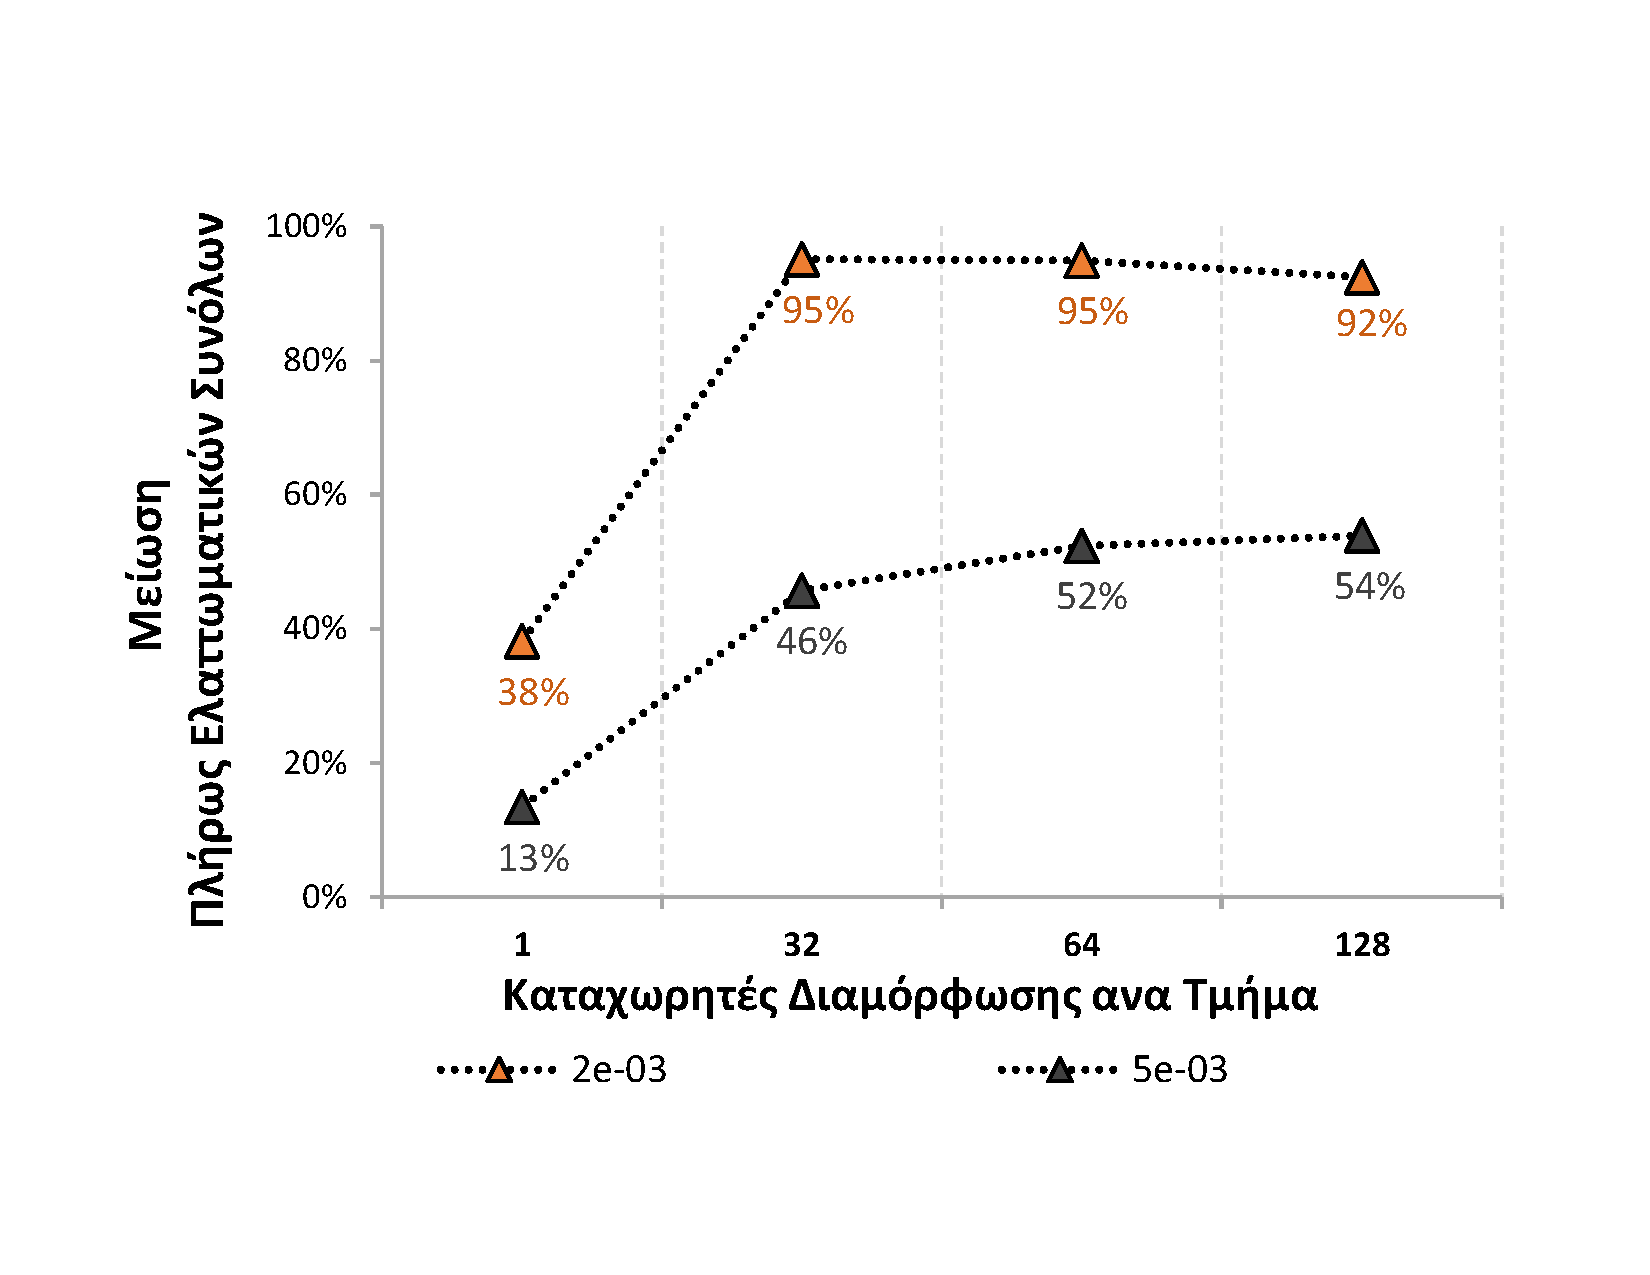
\includegraphics[width=0.99\linewidth, trim=2cm 2.9cm 1.8cm 3.5cm, clip=true]{\resultsDIR/chap6_BTB_ffsets_reduction_2048_2way.pdf}}
        \caption{ΠΠΠΔ 2048-πλαισίων/2-τρόπων}
        \label{fig:chap6_btb_ffsets_2048_2way}
    \end{subfigure}%
    \begin{subfigure}[t]{0.5\textwidth}
        \centering
        \fbox{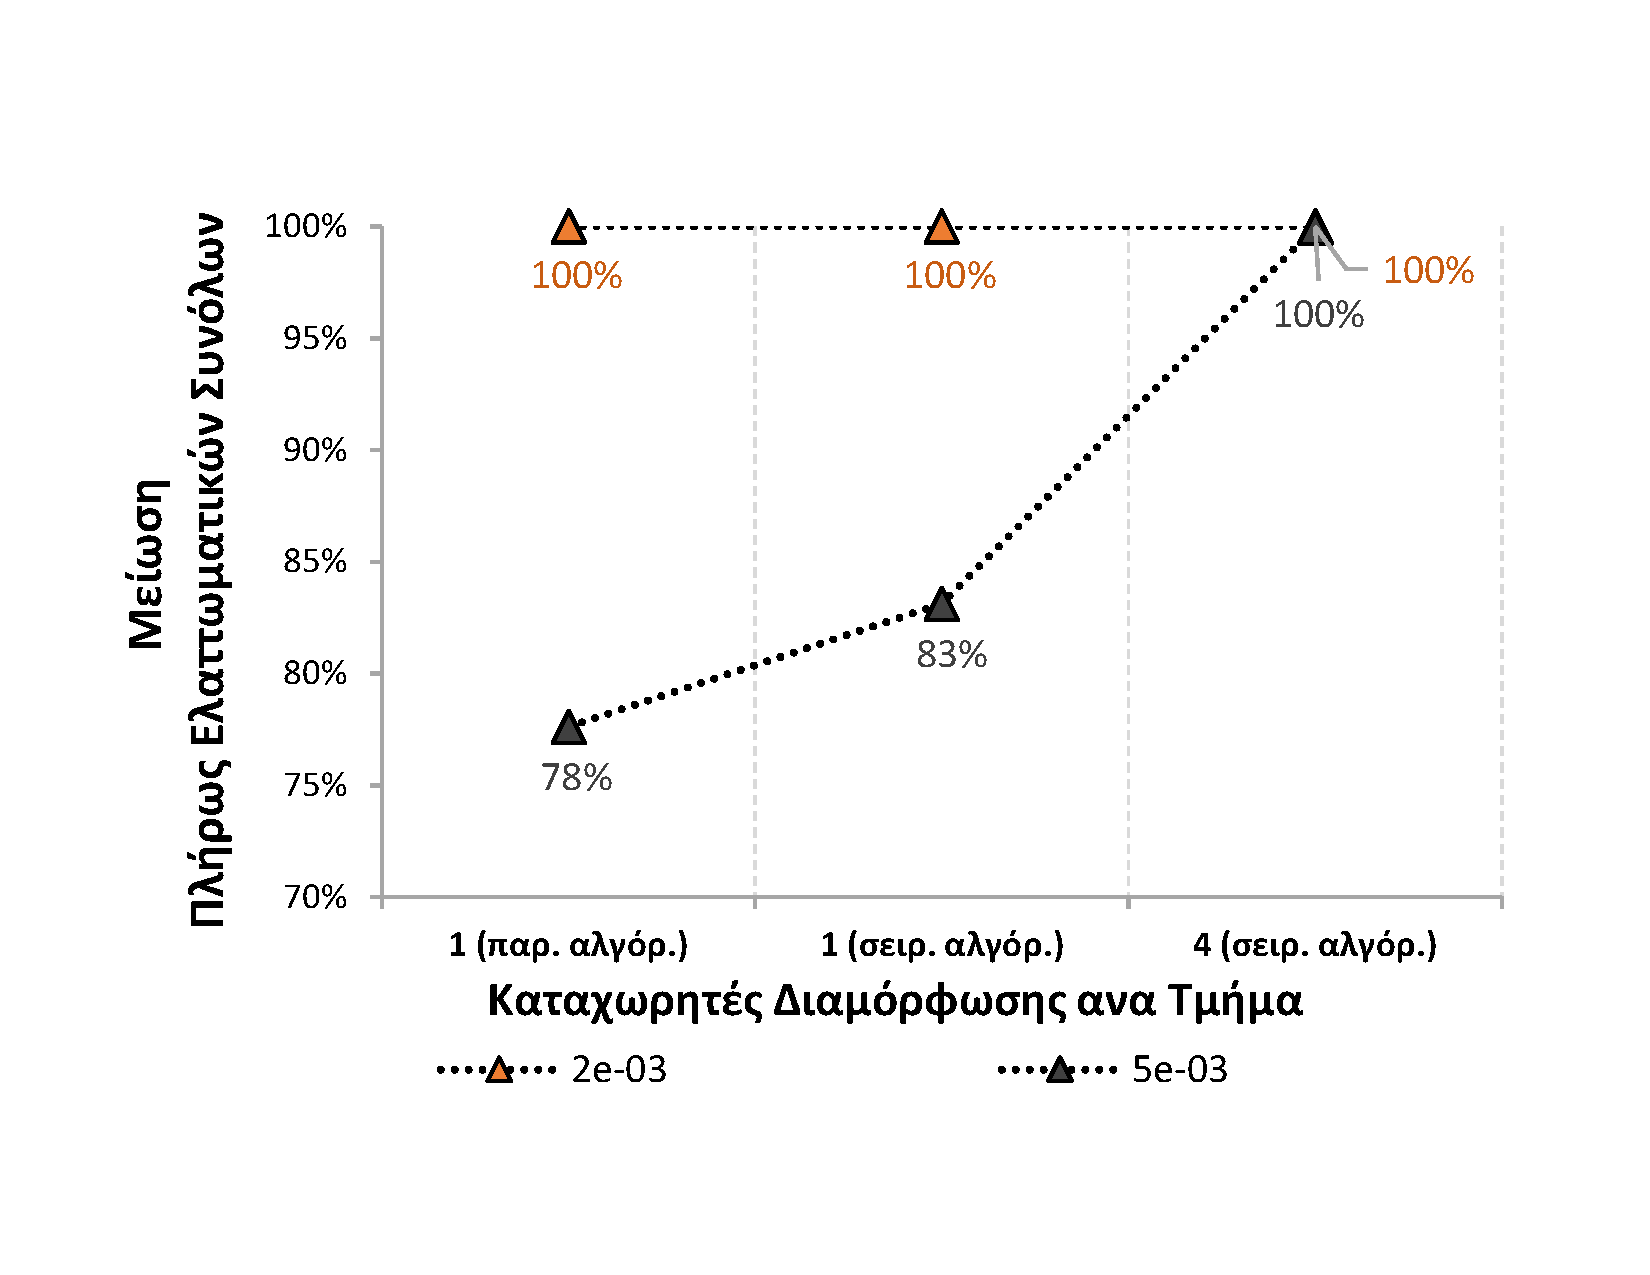
\includegraphics[width=0.99\linewidth, trim=2cm 2.9cm 1.8cm 3.5cm, clip=true]{\resultsDIR/chap6_BTB_ffsets_reduction_2048_4way.pdf}}
        \caption{ΠΠΠΔ 2048-πλαισίων/4-τρόπων}
        \label{fig:chap6_btb_ffsets_2048_4way}
    \end{subfigure}
    \caption{Μείωση των πλήρως ελαττωματικών πλαισίων με τη χρήση των προτεινόμενων μοντέλων ως προς το βασικό μοντέλο (υποπεριπτώσεις του Σχήματος \ref{fig:chap5_btb_ffsets_2048})}
    \label{fig:chap6_btb_ffsets_2048}
\end{figure}

Η μείωση της απόδοσης ισοδυναμεί με τη μείωση του ρυθμού ολοκλήρωσης εντολών (\ipc) η οποία υπολογίζεται από την εξίσωση:

\begin{equation}
    \label{eqn:chap6_IPCfaulty}
    \mathgr{Μείωση}\_IPC = \frac{IPC_\mathgr{χωρίς\_σφάλματα} - IPC_\mathgr{εξομοιούμενο\_μοντέλο\_με\_σφάλματα}}{IPC_\mathgr{χωρίς\_σφάλματα}}
\end{equation}

Τα αποτελέσματα αποτελούν τη μέση τιμή των 100 διαφορετικών εξομοιώσεων χαρτών σφαλμάτων. Το ποσοστό 0\% αντιστοιχεί σε μηδενική απώλεια απόδοσης (\ipc με σφάλματα στον Πίνακα Πρόβλεψης Προορισμού Διακλάδωσης = \ipc χωρίς σφάλματα στον Πίνακα Πρόβλεψης Προορισμού Διακλάδωσης) ενώ το ποσοστό 100\% ισοδυναμεί σε ολοκληρωτική απώλεια της απόδοσης (αδυναμία εκτέλεσης του προγράμματος). Η μεταβολή της απόδοσης παρουσιάζεται ξεχωριστά για κάθε μετροπρόγραμμα διότι η Μονάδα Δυναμικής Πρόβλεψης Διακλαδώσεων κατέχει διαφορετική βαρύτητα στο χρόνο εκτέλεσής τους. Τέλος, σε όλα τα γραφήματα της παρούσας ενότητας οι μπάρες κόκκινων αποχρώσεων αντιστοιχούν στα αποτελέσματα του βασικού μοντέλου ενώ οι μπάρες πράσινων αποχρώσεων σε αυτά του ενισχυμένου/βελτιστοποιημένου. Οι μελετώμενες πιθανότητες σφάλματος σε κάθε περίπτωση είναι $\expnum{2}$ και $\expnum{5}$ (Πιθανότητα Σφάλματος 1 και Πιθανότητα Σφάλματος 2 αντίστοιχα).

%----------------------------------------------------------%

\subsection{Αποτελέσματα Ενισχυμένου Σειριακού Μοντέλου}
\label{chap6_gem5SerialAlgResults}

Στα ακόλουθα γραφήματα παρουσιάζεται η σύγκριση μεταξύ βασικού και ενισχυμένου μοντέλου, όταν γίνεται χρήση του σειριακού αλγόριθμος. Όπως αναφέρεται και στον Πίνακα \ref{tab:chap6_LowPowerSimulations}, πραγματοποιήθηκαν εξομοιώσεις για οργανώσεις 2 και 4-τρόπων συνόλου συσχέτισης.
\par
Τα γραφήματα του Σχήματος \ref{fig:chap6_serial_2way_ipc} αναφέρονται τις περιπτώσεις Πίνακα Πρόβλεψης Προορισμού Διακλάδωσης 2-τρόπων. Όπως αναγράφεται στο πρώτο γράφημα \ref{fig:chap6_serial_2way_pail1_ipc}, στην πιθανότητα σφάλματος $\expnum{2}$, όπου τα ελαττωματικά πλαίσια αποτελούν το $19\%$ των συνολικών πλαισίων, η μείωση που υφίσταται ο ρυθμός ολοκλήρωσης εντολών (\ipc) εξαιτίας των σφαλμάτων στον Πίνακα Πρόβλεψης Προορισμού Διακλάδωσης ελαττώνεται κατά μέσο όρο από $8.6\%$ σε $5.9\%$. Επομένως, η τεχνική της λογικής μετάθεσης πλαισίων με τη χρήση ενός καταχωρητή ανά τμήμα σε συνδυασμό με τη χρήση του σειριακού αλγορίθμου, κατά μέσο όρο μπορεί να επαναφέρει το $32\%$ της απώλειας απόδοσης. Σε ορισμένες περιπτώσεις μετροπρογραμμάτων η βελτίωση που προσφέρει η τεχνική είναι ακόμα μεγαλύτερου μεγέθους, όπως για παράδειγμα στο \en{hmmer} όπου η μείωση της απόδοσης μεταβάλλεται από $9.9\%$ σε $3.1\%$ (επαναφορά κατά $68\%$).

\begin{figure}[!t]
    \centering
    \begin{subfigure}[t]{\textwidth}
        \centering
        \fbox{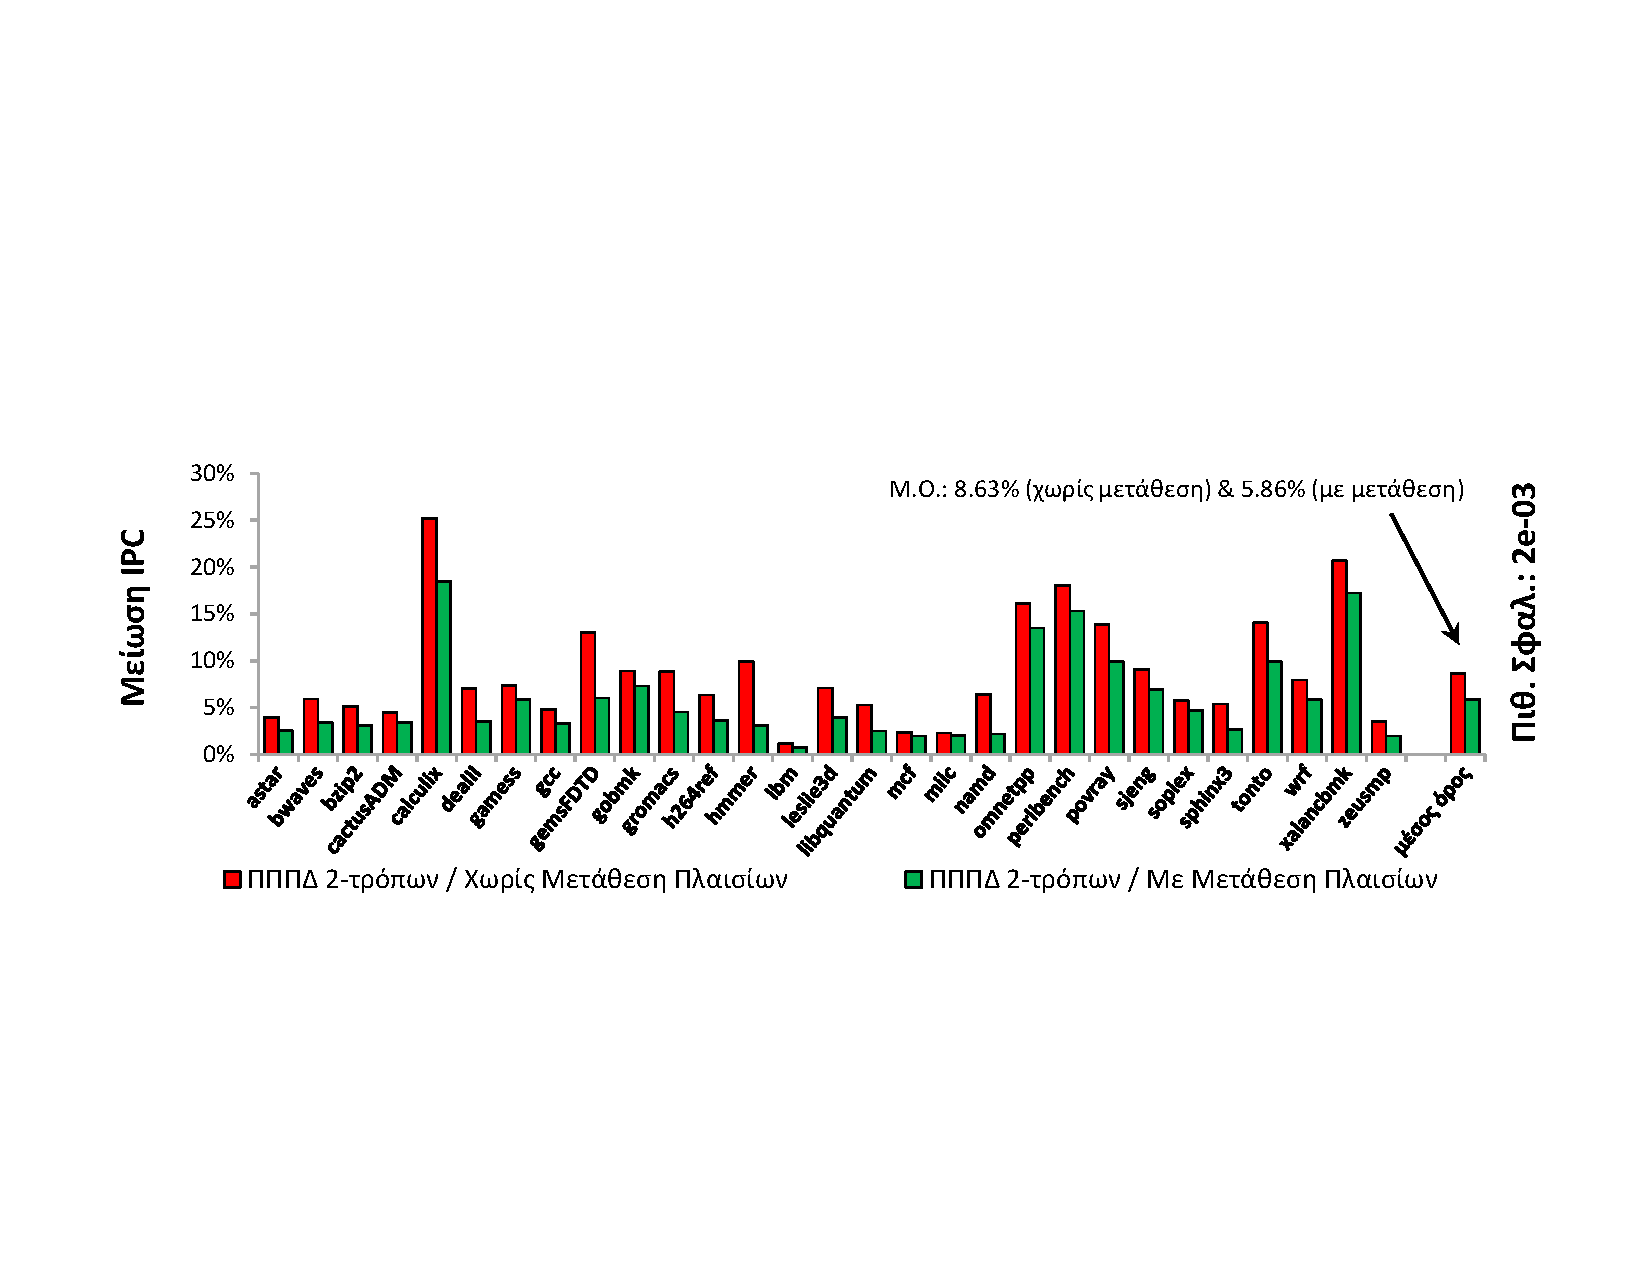
\includegraphics[width=\linewidth, trim=2cm 6.4cm 1.6cm 7.8cm, clip=true]{\resultsDIR/chap6_BTB_ipc_serial_w2_pfail1.pdf}}
        \caption{Πιθανότητα Σφάλματος 1}
        \label{fig:chap6_serial_2way_pail1_ipc}
    \end{subfigure}
    
    \begin{subfigure}[t]{\textwidth}
        \centering
        \fbox{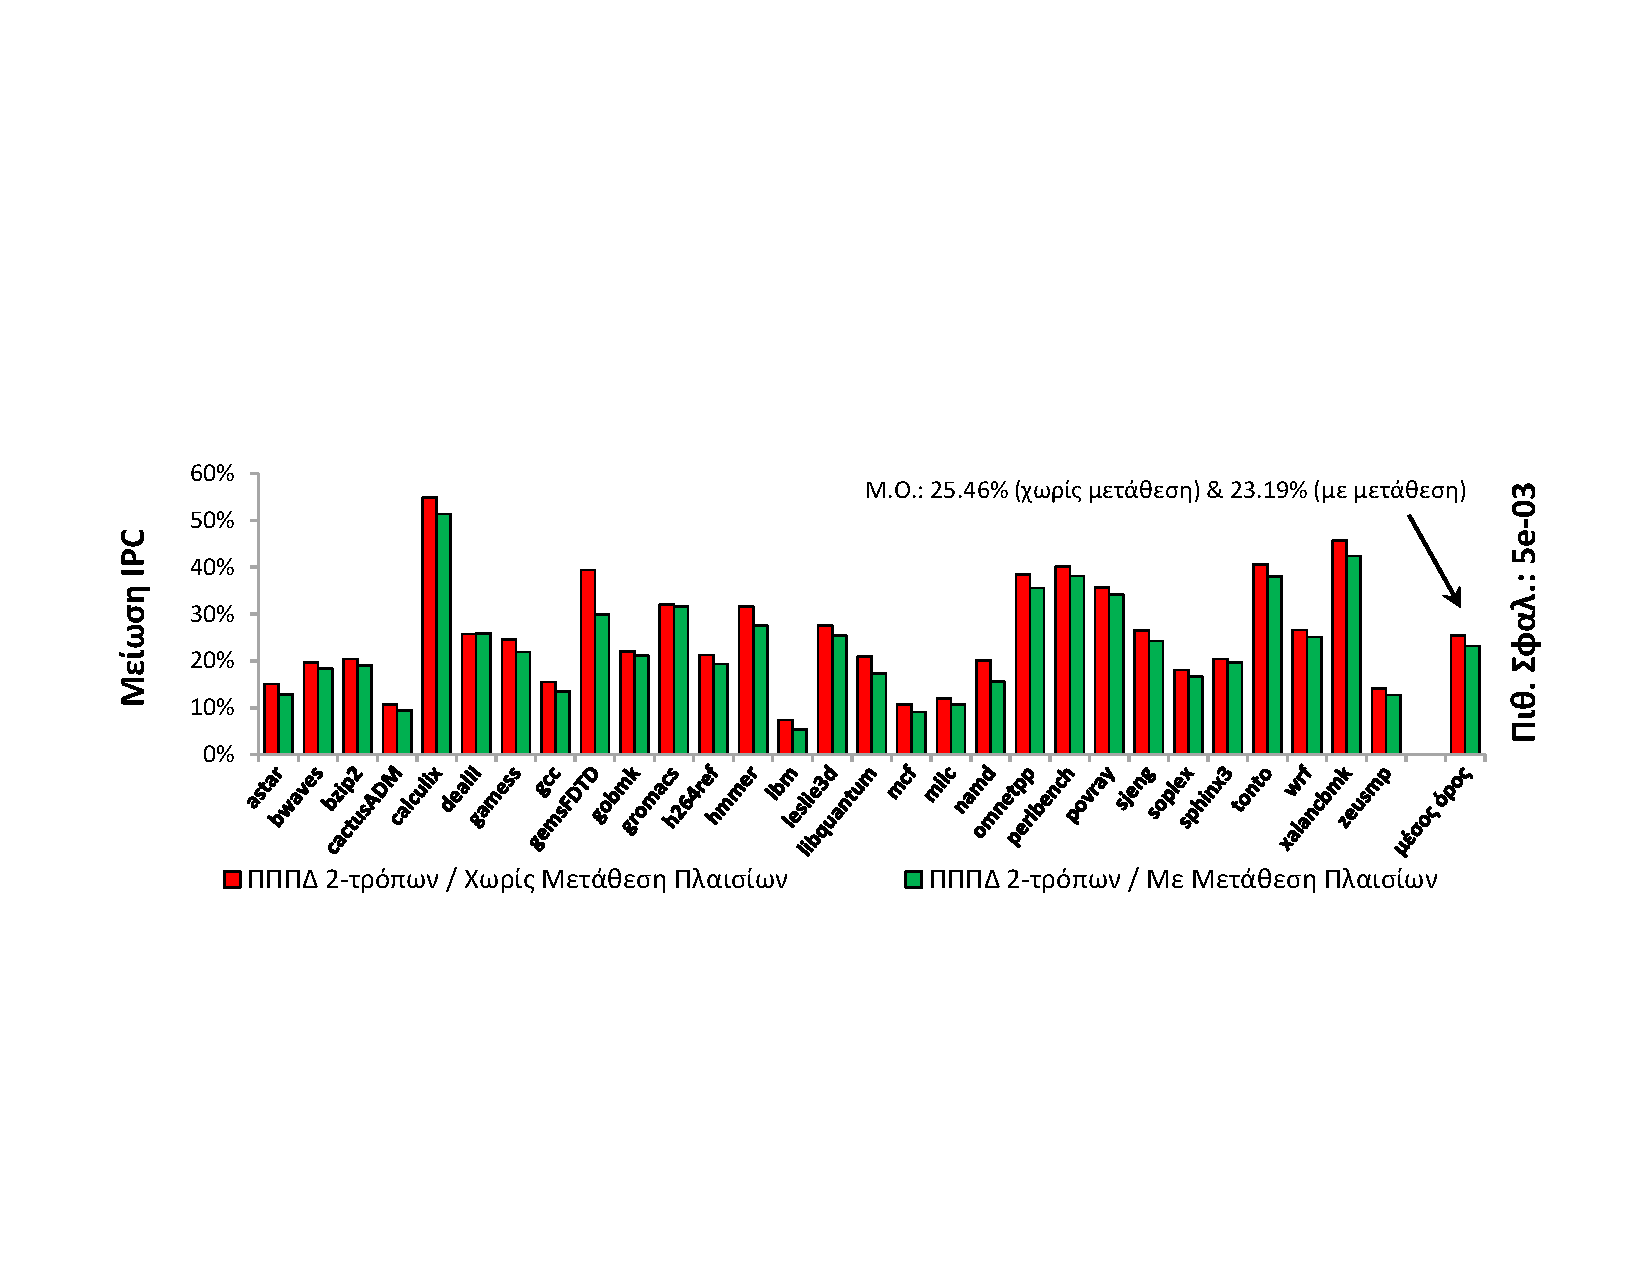
\includegraphics[width=\linewidth, trim=2cm 6.4cm 1.6cm 7.8cm, clip=true]{\resultsDIR/chap6_BTB_ipc_serial_w2_pfail2.pdf}}
        \caption{Πιθανότητα Σφάλματος 2}
        \label{fig:chap6_serial_2way_pail2_ipc}
    \end{subfigure}
    
    \caption{Αποτελέσματα με χρήση του σειριακού αλγορίθμου - (2-τρόπων ΠΠΠΔ)}
    \label{fig:chap6_serial_2way_ipc}
\end{figure}

Σύμφωνα με το γράφημα \ref{fig:chap6_serial_2way_pail2_ipc}, στην περίπτωση της πιθανότητας σφάλματος $\expnum{5}$, όπου τα ελαττωματικά πλαίσια ξεπερνούν το $40\%$, η μείωση του \ipc μεταβάλλεται κατά μέσο όρο από $25.5\%$ σε $23.2\%$ (επαναφορά κατά $8.9\%$). Η αδυναμία προσφοράς μεγαλύτερης επαναφοράς οφείλεται στον περιορισμό αναδιάταξης ενός μεγάλου πλήθους ελαττωματικών πλαισίων με αποδοτικό τρόπο όταν ο αριθμός τμημάτων είναι μικρός και χρησιμοποιείται ένας καταχωρητής ανά τμήμα (Σχήμα \ref{fig:chap5_btb_ffsets_2048_2way}: μείωση πλήρως ελαττωματικών συνόλων κατά 13\%). Παρόλα αυτά, υπάρχουν ορισμένες περιπτώσεις μετροπρογραμμάτων όπου η επαναφορά της απόδοσης είναι αρκετά σημαντική, όπως για παράδειγμα το \en{gemsFDTD} όπου η μείωση του \ipc μεταβάλλεται από $39.4\%$ σε $30\%$ (επαναφορά κατά $24\%$).
\par
Αντιστοίχως, το Σχήμα \ref{fig:chap6_serial_4way_ipc} αποτελείται από τις γραφικές παραστάσεις των περιπτώσεων Πινάκων Πρόβλεψης Προορισμού Διακλάδωσης 4-τρόπων. Το γράφημα \ref{fig:chap6_serial_4way_pail1_ipc} αναφέρεται στην περίπτωση της πιθανότητας σφάλματος $\expnum{2}$. H μείωση του \ipc ελαττώνεται κατά μέσο όρο από $1.20\%$ σε $0.63$\% ($47\%$ επαναφορά). Το σχετικά μικρό πλήθος ελαττωματικών συνόλων στην περίπτωση αυτή (λιγότερα από $20\%$) συνεπάγεται και την ελαχιστοποίηση της πιθανότητας να συνυπάρξουν 4 ελαττωματικά πλαίσια στο ίδιο σύνολο εξ αρχής. Για το λόγο αυτό η αρχική πτώση της απόδοσης δεν θεωρείται σημαντική, πλην ορισμένων περιπτώσεων όπως για παράδειγμα το \en{xalanbmk} όπου η μείωση της απόδοσης μεταβάλλεται από $8.5\%$ σε $6.5\%$ (επαναφορά κατά $23.7\%$).
\par
Στην πιθανότητα σφάλματος $\expnum{5}$, τα αποτελέσματα της οποίας παρουσιάζονται στο γράφημα \ref{fig:chap6_serial_4way_pail2_ipc}, η μείωση του \ipc ελαττώνεται κατά μέσο όρο από $8.1\%$ σε $3.8\%$. Συνεπώς η επαναφορά της απόδοσης είναι $52.9\%$. Παρότι το αρχικό ποσοστό μείωσης της απόδοσης δεν φαίνεται ιδιαίτερα σημαντικό, σε ορισμένα μετροπρογράμματα η βελτίωση είναι ιδιαίτερα σημαντική όπως για παράδειγμα το \en{calculix} όπου η μείωση της απόδοσης μεταβάλλεται από $19.6\%$ σε $7.6\%$ (επαναφορά κατά $61.2\%$).
\par
Στην περαιτέρω βελτίωση του ποσοστού επαναφοράς της απόδοσης σημαντικό ρόλο διαδραματίζει η χρήση περισσότερων Καταχωρητών Διαμόρφωσης ανά τμήμα, σύμφωνα με την μεθοδολογία που παρουσιάστηκε στην Ενότητα \ref{chap5_ImprovedMethod}.

\begin{figure}[!t]
    \centering
    \begin{subfigure}[t]{\textwidth}
        \centering
        \fbox{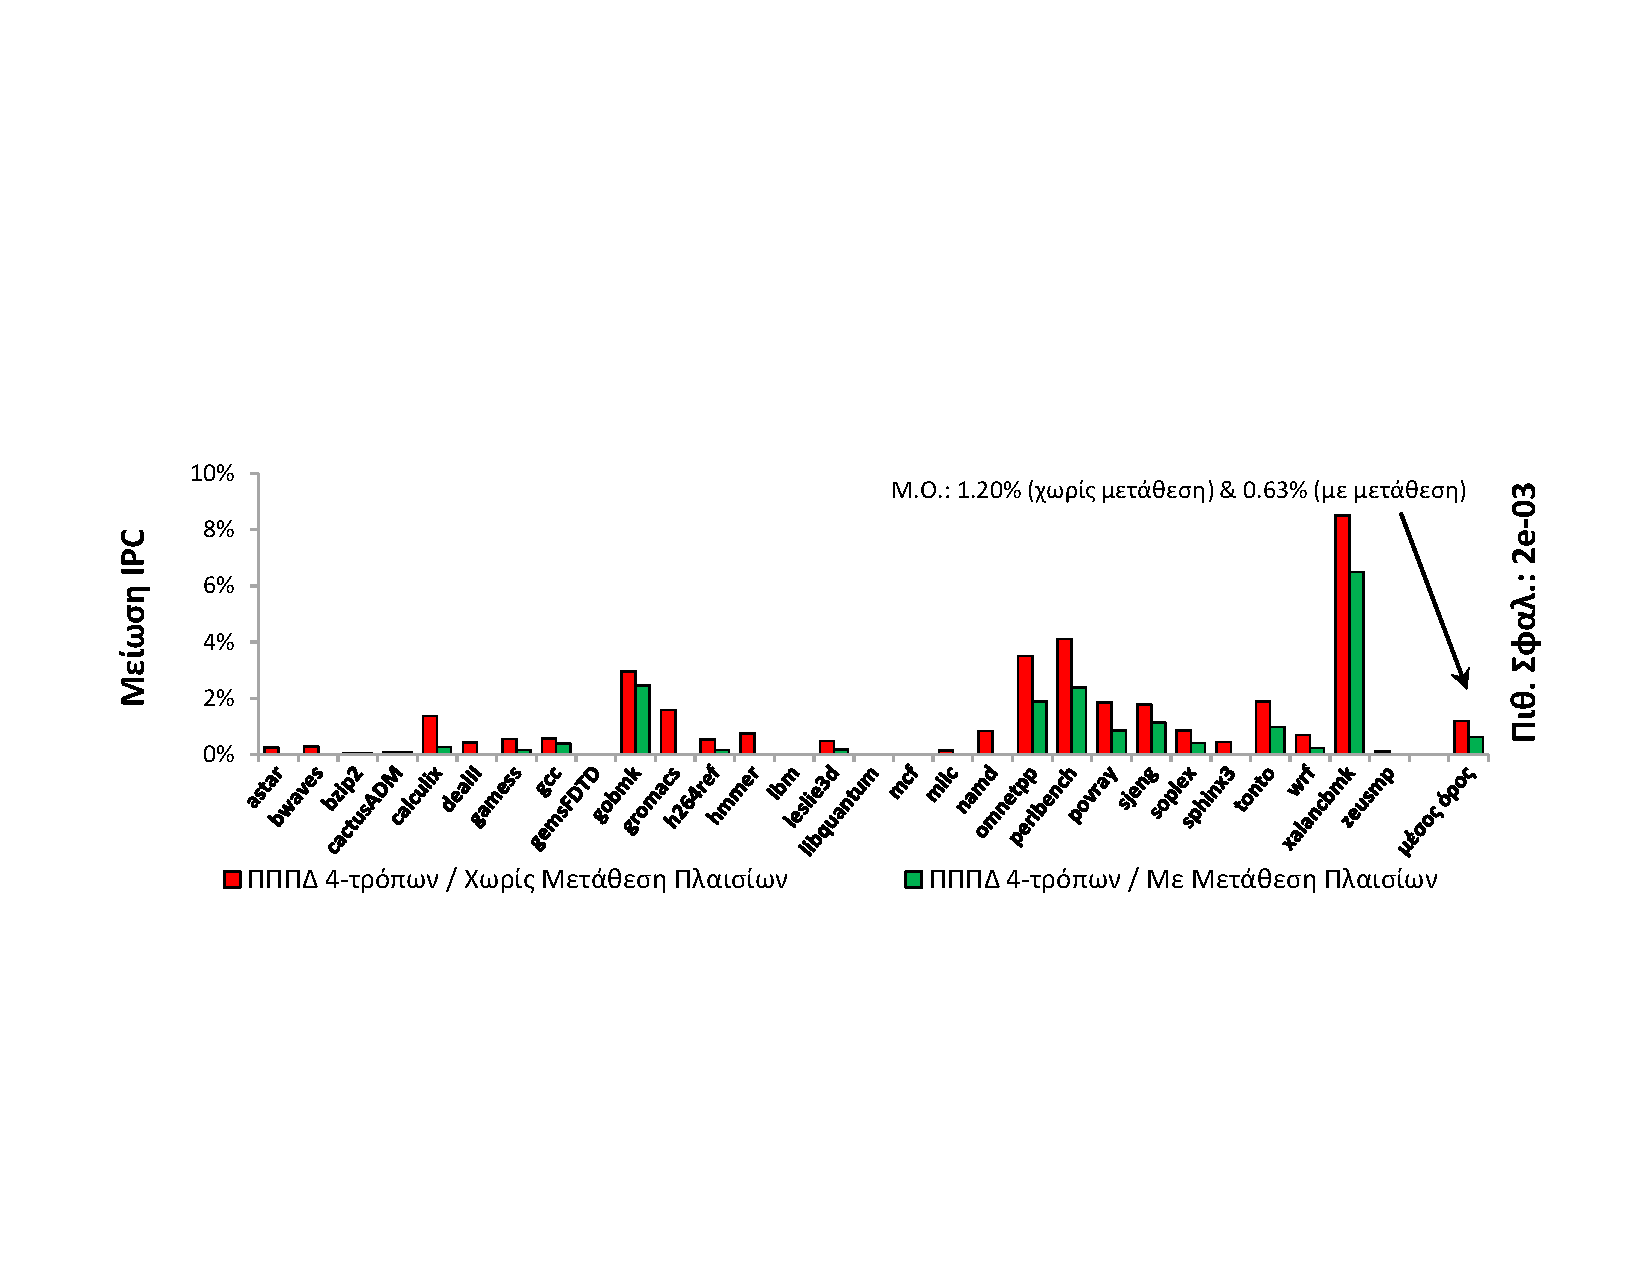
\includegraphics[width=\linewidth, trim=2cm 6.4cm 1.6cm 7.8cm, clip=true]{\resultsDIR/chap6_BTB_ipc_serial_w4_pfail1.pdf}}
        \caption{Πιθανότητα Σφάλματος 1}
        \label{fig:chap6_serial_4way_pail1_ipc}
    \end{subfigure}
    
    \begin{subfigure}[t]{\textwidth}
        \centering
        \fbox{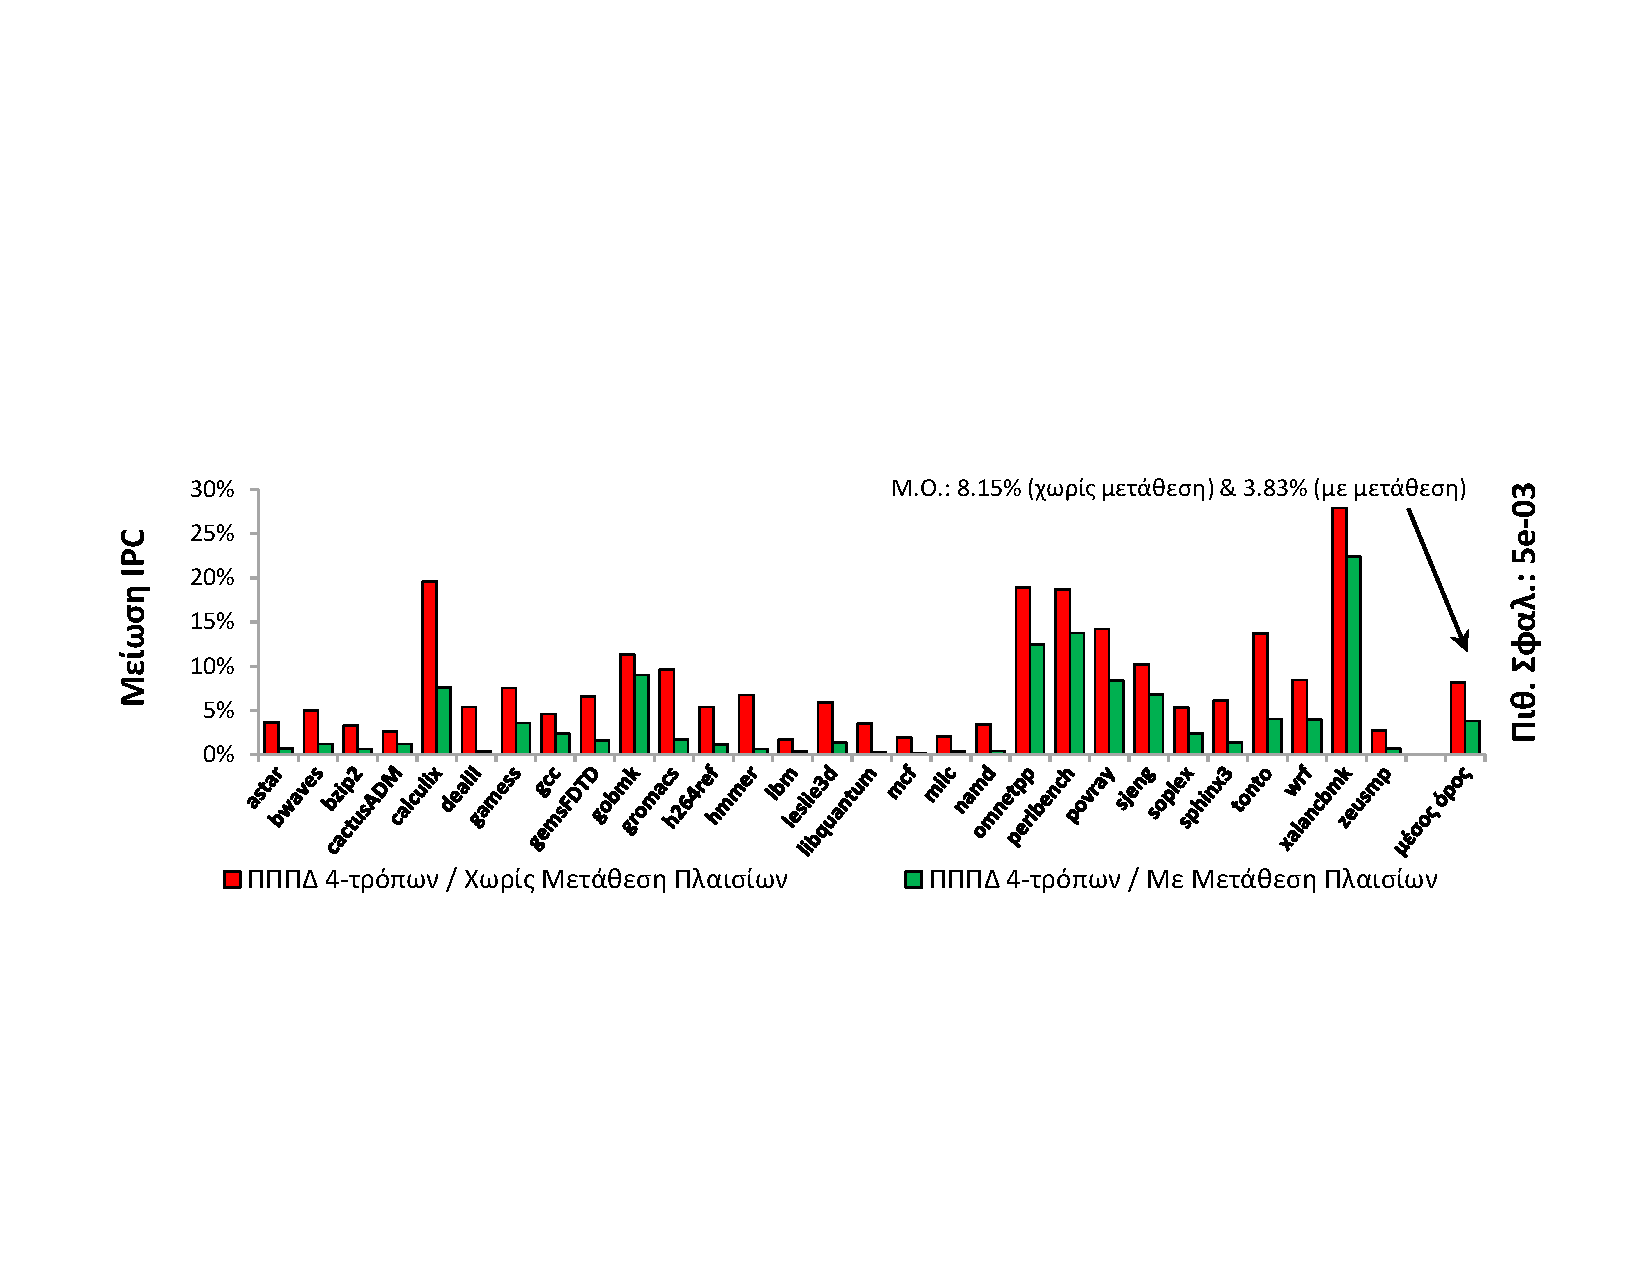
\includegraphics[width=\linewidth, trim=2cm 6.4cm 1.6cm 7.8cm, clip=true]{\resultsDIR/chap6_BTB_ipc_serial_w4_pfail2.pdf}}
        \caption{Πιθανότητα Σφάλματος 2}
        \label{fig:chap6_serial_4way_pail2_ipc}
    \end{subfigure}
    \caption{Αποτελέσματα με χρήση του σειριακού αλγορίθμου - (4-τρόπων ΠΠΠΔ)}
    \label{fig:chap6_serial_4way_ipc}
\end{figure}

%----------------------------------------------------------%

\subsection{Αποτελέσματα Ενισχυμένου Παράλληλου Μοντέλου}
\label{chap6_gem5ParallelAlgResults}

Στα γραφήματα του Σχήματος \ref{fig:chap6_parallel_4way_ipc} παρουσιάζεται η σύγκριση μεταξύ βασικού και ενισχυμένου μοντέλου όταν χρησιμοποιείται ο παράλληλος αλγόριθμος. Όπως αναφέρεται και στον Πίνακα \ref{tab:chap6_LowPowerSimulations}, πραγματοποιήθηκαν εξομοιώσεις για οργάνωση 4-τρόπων συνόλου συσχέτισης.
\par
Στην περίπτωση της πιθανότητας σφάλματος $\expnum{2}$ (γράφημα \ref{fig:chap6_parallel_4way_pail1_ipc}) η μείωση του \ipc εξαιτίας των σφαλμάτων στον Πίνακα Πρόβλεψης Προορισμού Διακλάδωσης ελαττώνεται κατά μέσο όρο από $1.20\%$ σε $0.73\%$. Επομένως, τεχνική της λογικής μετάθεσης πλαισίων ενός καταχωρητή ανά τμήμα, σε συνδυασμό με τη χρήση του παράλληλου αλγορίθμου μπορεί να επαναφέρει κατά $38.7\%$ την απόδοσης του υπερβαθμωτού επεξεργαστή, σε αντίθεση με την επαναφορά κατά $47\%$ που παρουσίασε η χρήση του σειριακού αλγορίθμου. Στην πιθανότητα σφάλματος $\expnum{5}$ (γράφημα \ref{fig:chap6_parallel_4way_pail2_ipc}) η μείωση του \ipc ελαττώνεται κατά μέσο όρο από $8.1\%$ σε $4.2\%$. Συνεπώς η επαναφορά της απόδοσης είναι $48\%$, από $52.9\%$ που ήταν με τη χρήση του σειριακού αλγορίθμου.
\par
Η διαφορά της βελτίωσης σε σχέση με την περίπτωση όπου χρησιμοποιείται ο σειριακός αλγόριθμος για τον υπολογισμό κατάλληλων τιμών ήταν αναμενόμενη σύμφωνα με την ανάλυση που πραγματοποιήθηκε στην Ενότητα \ref{chap5_AlgorithmResults}.

\begin{figure}[!t]
    \centering
    \begin{subfigure}[t]{\textwidth}
        \centering
        \fbox{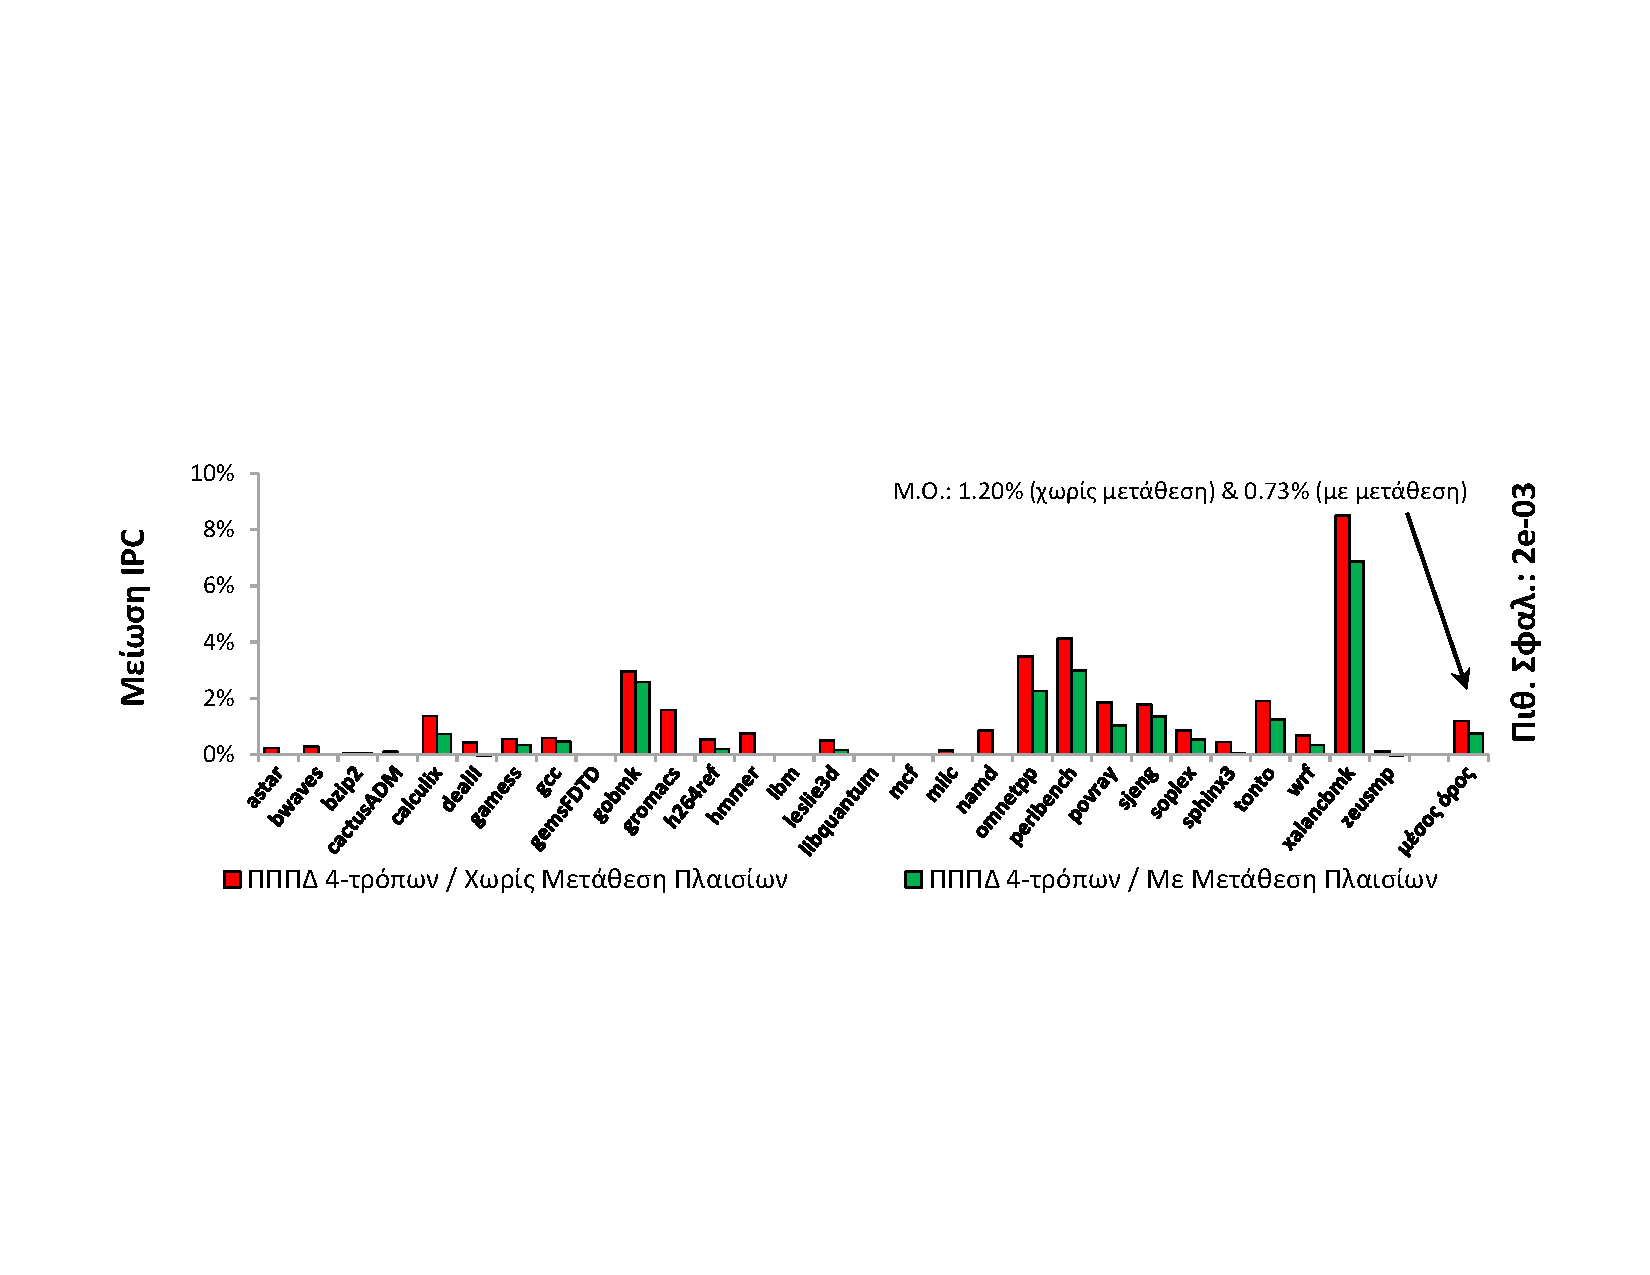
\includegraphics[width=\linewidth, trim=2cm 6.4cm 1.6cm 7.8cm, clip=true]{\resultsDIR/chap6_BTB_ipc_parallel_w4_pfail1.pdf}}
        \caption{Πιθανότητα Σφάλματος 1}
        \label{fig:chap6_parallel_4way_pail1_ipc}
    \end{subfigure}
    
    \begin{subfigure}[t]{\textwidth}
        \centering
        \fbox{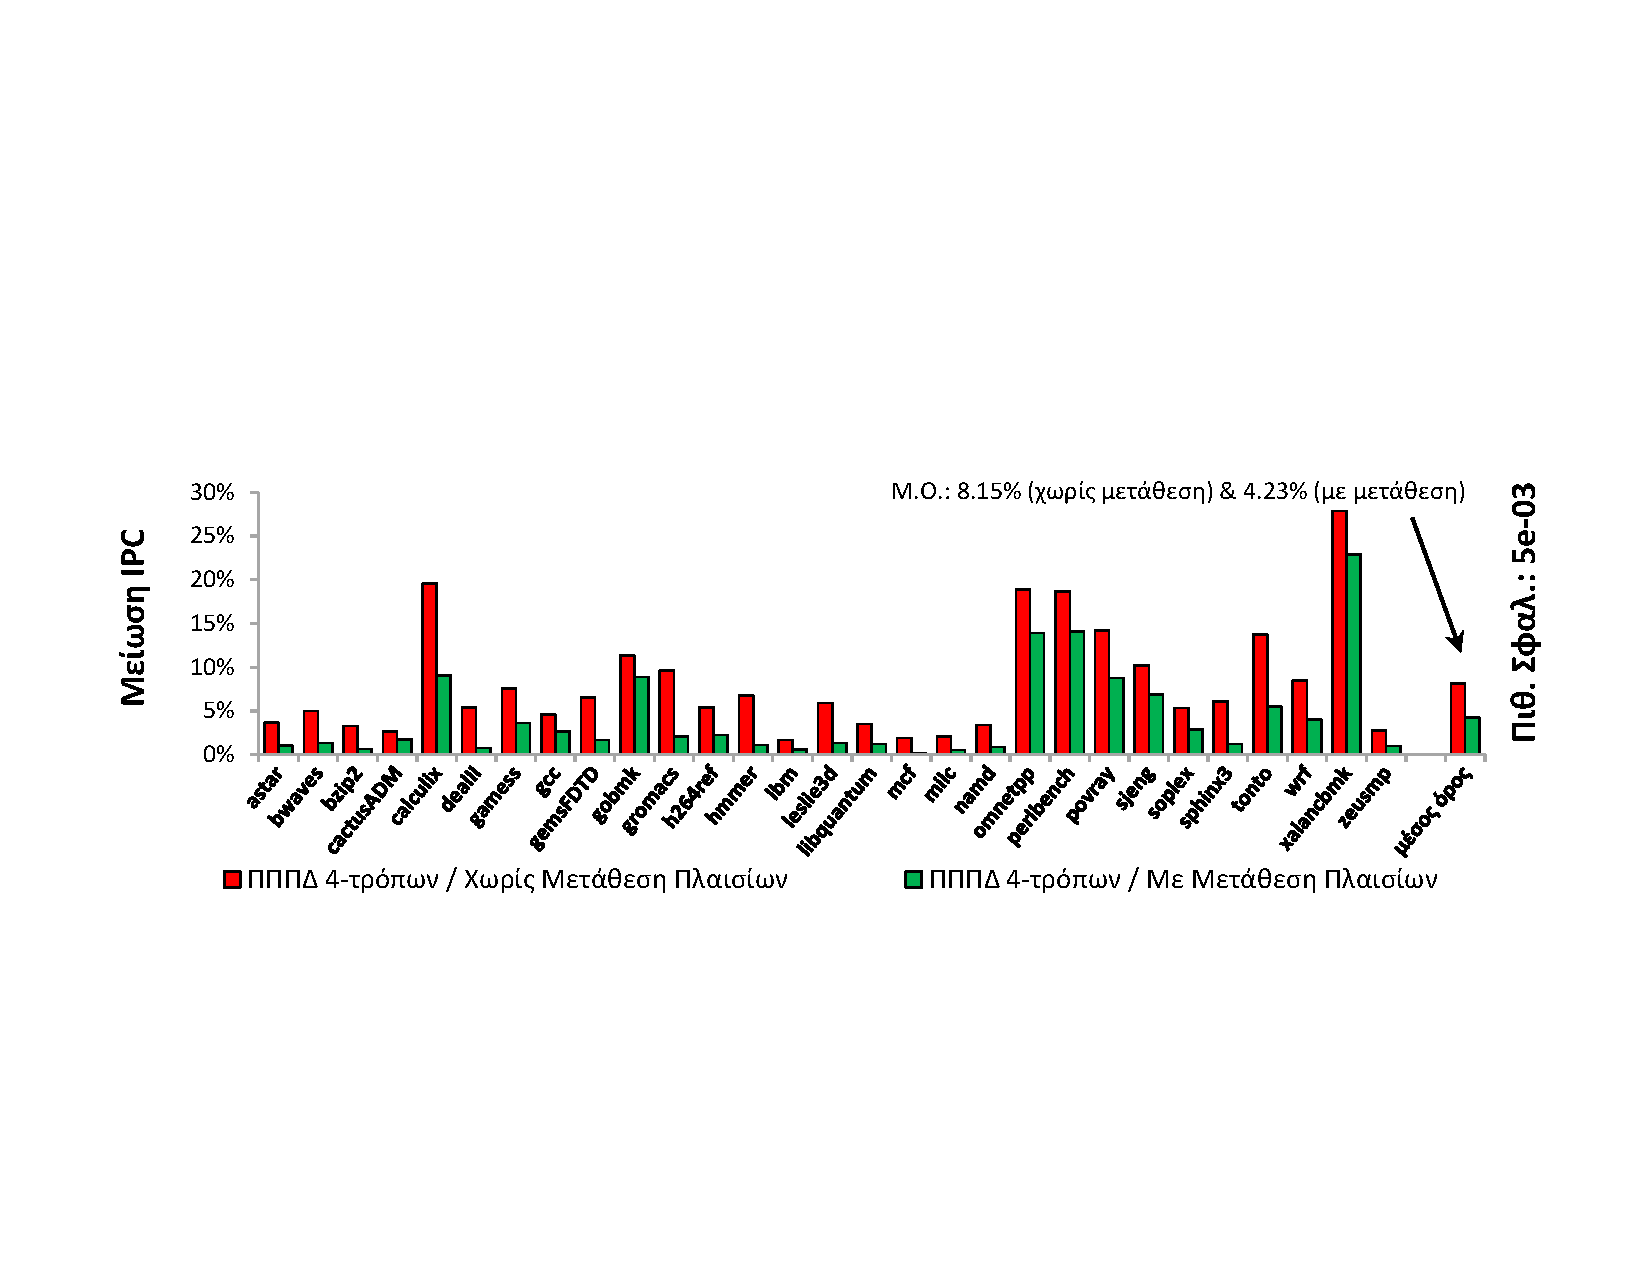
\includegraphics[width=\linewidth, trim=2cm 6.4cm 1.6cm 7.8cm, clip=true]{\resultsDIR/chap6_BTB_ipc_parallel_w4_pfail2.pdf}}
        \caption{Πιθανότητα Σφάλματος 2}
        \label{fig:chap6_parallel_4way_pail2_ipc}
    \end{subfigure}
    \caption{Αποτελέσματα με χρήση του παράλληλου αλγορίθμου}
    \label{fig:chap6_parallel_4way_ipc}
\end{figure}

%----------------------------------------------------------%

\subsection{Αποτελέσματα Βελτιστοποιημένου Σειριακού Μοντέλου}
\label{chap6_gem5OptimizedSerialAlgResults}

Η διάσπαση των τμημάτων σε υποτμήματα με τη χρήση ξεχωριστού Καταχωρητή Διαμόρφωσης σε κάθε ένα συμβάλει σημαντικά στην επίλυση του προβλήματος των πλήρως ελαττωματικών συνόλων. Τα αποτελέσματα της βελτιωμένης αυτής τεχνικής, παρουσιάζονται στα Σχήματα \ref{fig:chap6_optimized_serial_2way_ipc} και \ref{fig:chap6_optimized_serial_4way_ipc}, για οργανώσεις 2 και 4-τρόπων συνόλου συσχέτισης αντίστοιχα.
\par
Τα γραφήματα του Σχήματος \ref{fig:chap6_optimized_serial_2way_ipc} αναφέρονται στην περίπτωση οργάνωσης 2-τρόπων όπου κάθε τμήμα διασπάτε σε 64 υποτμήματα και επομένως κάθε Καταχωρητής Διαμόρφωσης συμβάλει στη δημιουργία 16 λογικών συνόλων. Στην πιθανότητα σφάλματος $\expnum{2}$, όπου η μείωση των πλήρως ελαττωματικών συνόλων αγγίζει το 95\% (Σχήμα \ref{fig:chap6_btb_ffsets_2048}), η μείωση του \ipc εξαιτίας των σφαλμάτων ελαττώνεται κατά μέσο όρο από $8.6\%$ σε $2.7\%$ (γράφημα \ref{fig:chap6_optimized_serial_2way_pail1_ipc}). Επομένως η επαναφορά της απόδοσης κατά μέσο όρο θα είναι $69\%$, από $32\%$ που ήταν με τη χρήση ενός μόνο καταχωρητή ανά τμήμα στην περίπτωση του ενισχυμένου σειριακού μοντέλου. Όπως φανερώνεται και από το γράφημα, σε ορισμένες περιπτώσεις μετροπρογραμμάτων επιτυγχάνεται πλήρης επαναφορά της απόδοσης όπως για παράδειγμα το \en{dealii} ($0\%$ μείωση του \ipc όταν εφαρμόζεται η τεχνική).
\par
Αντίστοιχα, στην περίπτωση της πιθανότητας σφάλματος $\expnum{5}$ (γράφημα \ref{fig:chap6_optimized_serial_2way_pail2_ipc}), όπου τα πλήρως ελαττωματικά σύνολα μειώνονται κατά 52\%, η μείωση του \ipc ελαττώνεται κατά μέσο όρο από $25.5\%$ σε $15.9\%$. Επομένως η επαναφορά της απόδοσης θα είναι $38\%$, από $9\%$ που ήταν με τη χρήση ενισχυμένου σειριακού μοντέλου. Σε αυτή την περίπτωση το μετροπρόγραμμα \en{gemsFDTD} εμφανίζει τη μεγαλύτερη βελτίωση καθώς η μείωση της απόδοσης μεταβάλλεται από $39.4\%$ σε $17.3\%$ (επαναφορά κατά $56\%$).

\begin{figure}[!t]
    \centering
    \begin{subfigure}[t]{\textwidth}
        \centering
        \fbox{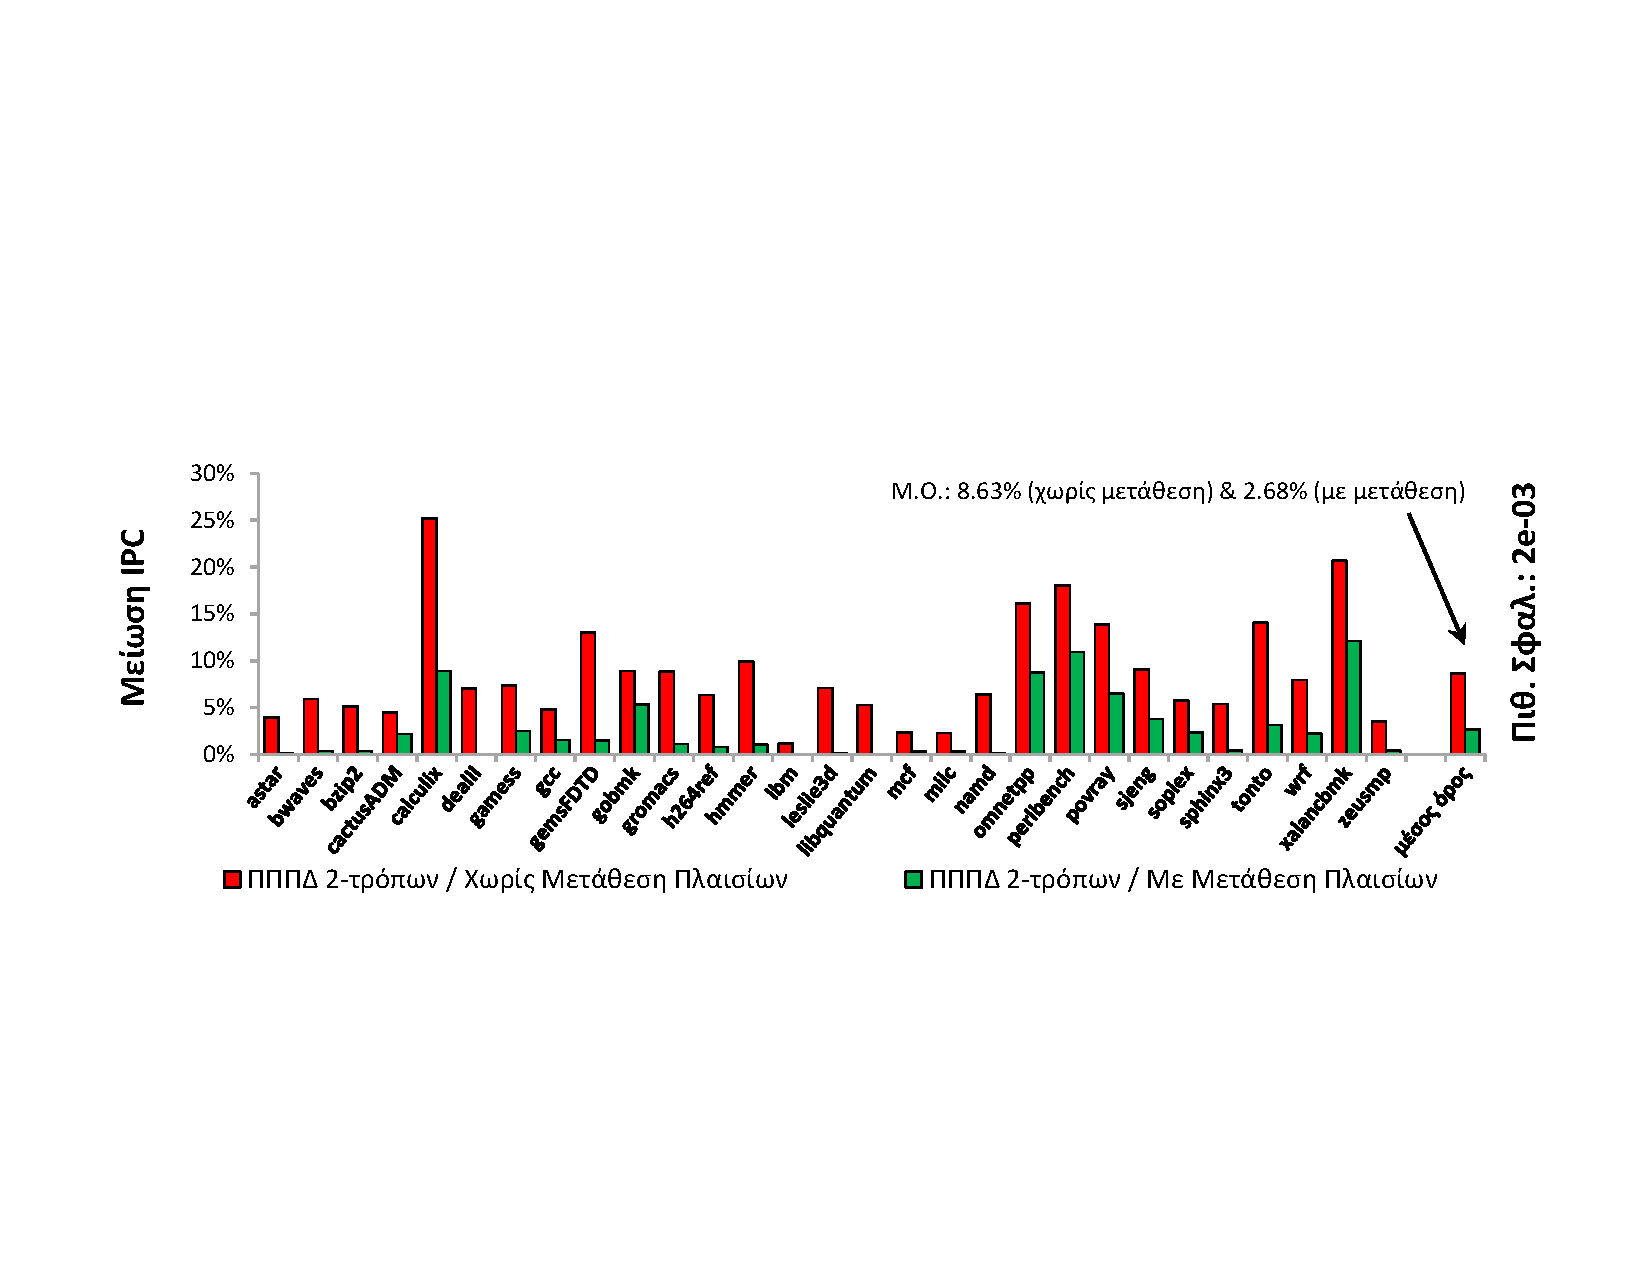
\includegraphics[width=\linewidth, trim=2cm 6.4cm 1.6cm 7.8cm, clip=true]{\resultsDIR/chap6_BTB_ipc_optimized_serial_w2_pfail1.pdf}}
        \caption{Πιθανότητα Σφάλματος 1}
        \label{fig:chap6_optimized_serial_2way_pail1_ipc}
    \end{subfigure}
    
    \begin{subfigure}[t]{\textwidth}
        \centering
        \fbox{\includegraphics[width=\linewidth, trim=2cm 6.4cm 1.6cm 7.8cm, clip=true]{\resultsDIR/chap6_BTB_ipc_optimized_serial_w2_pfail2.pdf}}
        \caption{Πιθανότητα Σφάλματος 2}
        \label{fig:chap6_optimized_serial_2way_pail2_ipc}
    \end{subfigure}
    
    \caption{Αποτελέσματα με διάσπαση σε υποτμήματα και χρήση του σειριακού αλγορίθμου (2-τρόπων ΠΠΠΔ)}
    \label{fig:chap6_optimized_serial_2way_ipc}
\end{figure}

Το Σχήμα \ref{fig:chap6_optimized_serial_4way_ipc} αποτελείται από τις αντίστοιχες γραφικές παραστάσεις των περιπτώσεων Πινάκων Πρόβλεψης Προορισμού Διακλάδωσης 4-τρόπων. Τα αποτελέσματα της πιθανότητας σφάλματος $\expnum{2}$ παραλείπονται καθώς η χρήση τεσσάρων καταχωρητών ανά τμήμα κατά μέσο όρο προσφέρει ισοδύναμη επαναφορά της απόδοσης με την περίπτωση χρήση ενός καταχωρητή ανά τμήμα που παρουσιάστηκε στο ενισχυμένο σειριακό μοντέλο.
\par
Όταν η πιθανότητα σφάλματος είναι $\expnum{5}$ η χρήση μεγαλύτερου πλήθους καταχωρητών συμβάλει στην περαιτέρω βελτίωση τόσο της κατανομής όσο και της απόδοσης. Συγκεκριμένα, με τη χρήση 4 καταχωρητών ανά τμήμα, όπου εξασφαλίζεται η ολοκληρωτική εξάλειψη των πλήρως ελαττωματικών πλαισίων (Σχήμα \ref{fig:chap6_btb_ffsets_2048}), η μείωση του \ipc ελαττώνεται κατά μέσο όρο από $8.1\%$ σε $2.4\%$. Συνεπώς η επαναφορά της απόδοσης είναι $70\%$, από $52.9\%$ που ήταν με τη χρήση ενός καταχωρητή ανά τμήμα σε συνδυασμό με τη χρήση του σειριακού αλγορίθμου. Αξίζει να σημειωθεί πως και σε αυτή την περίπτωση πολλά μετροπρογράμματα αποκομίζουν σημαντικά οφέλη στην απόδοση, όπως για παράδειγμα το \en{calculix} όπου η μείωση της απόδοσης μεταβάλλεται από $19.6\%$ σε $3.3\%$ (επαναφορά κατά $83.1\%$).

\begin{figure}[!t]
    \centering
    \fbox{\includegraphics[width=\linewidth, trim=2cm 6.4cm 1.6cm 7.8cm, clip=true]{\resultsDIR/chap6_BTB_ipc_optimized_serial_w4_pfail2.pdf}}
    \caption{Αποτελέσματα με διάσπαση σε υποτμήματα και χρήση του σειριακού αλγορίθμου (4-τρόπων ΠΠΠΔ / Πιθανότητα Σφάλματος 2}
    \label{fig:chap6_optimized_serial_4way_ipc}
\end{figure}

%----------------------------------------------------------%

\section{Αποτελέσματα \mcpat}
\label{chap6_mcpatResults}

Σύμφωνα με τα αποτελέσματα της Ενότητας \ref{chap6_gem5Results}, η χρήση της προτεινόμενης μεθόδου με τις παραλλαγές που παρουσιάστηκαν εξασφαλίζει προστασία σε ικανοποιητικό επίπεδο ενάντια στην απώλεια απόδοσης, εξαιτίας της ύπαρξης σφαλμάτων στον Πίνακα Πρόβλεψης Προορισμού Διακλάδωσης. Το μέγεθος αυτής της βελτίωσης διαφέρει μεταξύ των μετροπρογραμμάτων και αυτό οφείλεται στη διαφορετική συμπεριφορά κάθε μετροπρογράμματος. Παρόλα αυτά, όταν ο υπερβαθμωτός επεξεργαστής λειτουργεί σε κατάσταση χαμηλής κατανάλωσης σημαντικότερη παράμετρο αξιολόγηση δεν αποτελεί η απόδοση σε επεξεργαστική ισχύ, αλλά η δυνατότητα μείωσης της συνολικής καταναλισκόμενης ενέργειας. Για το λόγο αυτό εκτελείται και η αντίστοιχη αξιολόγηση της προτεινόμενης μεθόδου, σε σχέση με το βασικό μοντέλο.
\par
Στην παρούσα αξιολόγηση υπολογίζεται η ενέργεια που δαπανάται για τη συνολική εκτέλεση ενός προγράμματος (Γινόμενο Ενέργειας-Καθυστέρησης - \edp) για κάθε εξομοιούμενο μοντέλο,
διότι η προτεινόμενη τεχνική δεν προσφέρει μείωση της κατανάλωσης ανά χρονική στιγμή αλλά μείωση του συνολικού χρόνου εκτέλεσης ενός προγράμματος, το οποίο συνεπάγεται τη μείωση της συνολικής κατανάλωσης.
\par
Στα ακόλουθα γραφήματα παρουσιάζεται η αύξηση της συνολικής κατανάλωσης που αντιστοιχεί στην αύξηση του \edp, το μέγεθος της οποίας υπολογίζεται από την εξίσωση:

\begin{equation}
    \label{eqn:chap6_EDPfaulty}
    \mathgr{Μείωση}\_EDP = \frac{EDP_\mathgr{χωρίς\_σφάλματα} - EDP_\mathgr{εξομοιούμενο\_μοντέλο\_με\_σφάλματα}}{EDP_\mathgr{χωρίς\_σφάλματα}}
\end{equation}

Σε αντίθεση με τα γραφήματα του \ipc που παρουσιάστηκαν έως τώρα, η αύξηση του \edp αποτελεί αρνητικό παράγοντα και επομένως ζητούμενο είναι η ελάττωση της. Το ποσοστό 0\% αντιστοιχεί σε μηδενική αύξηση της ενέργειας που πρόκειται να καταναλωθεί για την εκτέλεση του αντίστοιχου μετροπρογράμματος, εξαιτίας των σφαλμάτων (\edp με σφάλματα = \edp χωρίς σφάλματα). Όπως και στα γραφήματα της απόδοσης, η μεταβολή της κατανάλωσης παρουσιάζεται ξεχωριστά για κάθε μετροπρόγραμμα, με τις μπάρες πορτοκαλί αποχρώσεων να αντιστοιχούν στα αποτελέσματα του βασικού μοντέλου ενώ αυτές των μπλε αποχρώσεων στα αποτελέσματα του ενισχυμένου/βελτιστοποιημένου. Οι μελετώμενες πιθανότητες σφάλματος σε κάθε περίπτωση, όπως και στην περίπτωση της απόδοσης, είναι $\expnum{2}$ και $\expnum{5}$ (Πιθανότητα Σφάλματος 1 και Πιθανότητα Σφάλματος 2 αντίστοιχα).

%----------------------------------------------------------%

\subsection{Αποτελέσματα Ενισχυμένου Σειριακού Μοντέλου}
\label{chap6_mcpatSerialAlgResults}

Στα ακόλουθα Σχήματα \ref{fig:chap6_serial_2way_edp} και \ref{fig:chap6_serial_4way_edp} παρουσιάζεται η σύγκριση μεταξύ βασικού και ενισχυμένου μοντέλου όταν χρησιμοποιείται ο σειριακός αλγόριθμος για τις δύο οργανώσεις συνόλου συσχέτισης.
\par
Στην πιθανότητα σφάλματος $\expnum{2}$ και οργάνωση 2-τρόπων (γράφημα \ref{fig:chap6_serial_2way_pail1_edp}), η αύξηση του \edp ελαττώνεται κατά μέσο όρο από $28.76\%$ σε $16.85\%$. Επομένως η επαναφορά της κατανάλωσης είναι $41\%$. Μεταξύ των μετροπρογραμμάτων εμφανίζονται και περιπτώσεις όπου η επαναφορά είναι αρκετά μεγαλύτερη του μέσου όρου όπως για παράδειγμα το \en{gemsFDTD} όπου η αύξηση μεταβάλλεται από $120.74\%$ σε $44.56\%$ (επαναφορά κατά $63\%$).
\par
Αντίστοιχα, στο γράφημα \ref{fig:chap6_serial_2way_pail2_edp} παρουσιάζονται τα αποτελέσματα της πιθανότητας σφάλματος $\expnum{5}$ και οργάνωση 2-τρόπων. Η αύξηση του \edp σε αυτή την περίπτωση ελαττώνεται κατά μέσο όρο από $124.33\%$ σε $104.24\%$. Επομένως η επαναφορά της κατανάλωσης είναι $16\%$. Παρόλα αυτά, στο μετροπρόγραμμα \en{gemsFDTD} εμφανίζεται μεταβολή της αύξηση από $517.28\%$ σε $314.34\%$ (επαναφορά κατά $39\%$).

\begin{figure}[!t]
    \centering
    \begin{subfigure}[t]{\textwidth}
        \centering
        \fbox{\includegraphics[width=\linewidth, trim=2cm 6.4cm 1.6cm 7.7cm, clip=true]{\resultsDIR/chap6_BTB_edp_serial_w2_pfail1.pdf}}
        \caption{Πιθανότητα Σφάλματος 1}
        \label{fig:chap6_serial_2way_pail1_edp}
    \end{subfigure}
    
    \begin{subfigure}[t]{\textwidth}
        \centering
        \fbox{\includegraphics[width=\linewidth, trim=2cm 6.4cm 1.6cm 7.7cm, clip=true]{\resultsDIR/chap6_BTB_edp_serial_w2_pfail2.pdf}}
        \caption{Πιθανότητα Σφάλματος 2}
        \label{fig:chap6_serial_2way_pail2_edp}
    \end{subfigure}
    
    \caption{Αποτελέσματα με χρήση του σειριακού αλγορίθμου - (2-τρόπων ΠΠΠΔ)}
    \label{fig:chap6_serial_2way_edp}
\end{figure}

Όταν η οργάνωση είναι 4-τρόπων η ελάττωση των επιπτώσεων στην κατανάλωση εξαιτίας των σφαλμάτων στον Πίνακα Πρόβλεψης Προορισμού Διακλάδωσης γίνεται ευκολότερη. Στην πιθανότητα σφάλματος $\expnum{2}$ (γράφημα \ref{fig:chap6_serial_4way_pail1_edp}), η αύξηση του \edp ελαττώνεται κατά μέσο όρο από $2.93\%$ σε $1.34\%$ (επαναφορά κατά $54\%$). Στο μετροπρόγραμμα \en{gromacs} παρουσιάζεται η μεγαλύτερη βελτίωση καθώς η αύξηση της κατανάλωσης μεταβάλλεται από $11.92\%$ σε μόλις $0.11\%$ (επαναφορά κατά $99\%$). Συνεπώς η χρήση της προτεινόμενης τεχνικής έκανε το συγκεκριμένο μετροπρόγραμμα να εκτελεστεί με το ίδιο ενεργειακό κόστος που θα είχε εάν όλα τα πλαίσια του Πίνακα Πρόβλεψης Προορισμού Διακλάδωσης λειτουργούσαν σωστά.
\par
Στην πιθανότητα σφάλματος $\expnum{5}$ (γράφημα \ref{fig:chap6_serial_4way_pail2_edp}), η αύξηση του \edp ελαττώνεται κατά μέσο όρο από $25.92\%$ σε $9.87\%$ (επαναφορά κατά $62\%$). Όπως και στην χαμηλότερη πιθανότητα σφάλματος, το μετροπρόγραμμα \en{gromacs} παρουσιάζει τη μεγαλύτερη βελτίωση καθώς η αύξηση της κατανάλωσης μεταβάλλεται από $78.69\%$ σε $9.39\%$ (επαναφορά κατά $88\%$).

\begin{figure}[!t]
    \centering
    \begin{subfigure}[t]{\textwidth}
        \centering
        \fbox{\includegraphics[width=\linewidth, trim=2cm 6.4cm 1.6cm 7.7cm, clip=true]{\resultsDIR/chap6_BTB_edp_serial_w4_pfail1.pdf}}
        \caption{Πιθανότητα Σφάλματος 1}
        \label{fig:chap6_serial_4way_pail1_edp}
    \end{subfigure}
    
    \begin{subfigure}[t]{\textwidth}
        \centering
        \fbox{\includegraphics[width=\linewidth, trim=2cm 6.4cm 1.6cm 7.7cm, clip=true]{\resultsDIR/chap6_BTB_edp_serial_w4_pfail2.pdf}}
        \caption{Πιθανότητα Σφάλματος 2}
        \label{fig:chap6_serial_4way_pail2_edp}
    \end{subfigure}
    \caption{Αποτελέσματα με χρήση του σειριακού αλγορίθμου - (4-τρόπων ΠΠΠΔ)}
    \label{fig:chap6_serial_4way_edp}
\end{figure}

%----------------------------------------------------------%

\subsection{Αποτελέσματα Ενισχυμένου Παράλληλου Μοντέλου}
\label{chap6_mcpatParallelAlgResults}

Όπως αποδείχθηκε, η χρήση του παράλληλου αλγορίθμου δεν προσφέρει καλύτερα αποτελέσματα στην απόδοση από αυτή του σειριακού και επομένως δεν αναμένονται καλύτερα αποτελέσματα στην κατανάλωση. Παρόλα αυτά, αξίζει να γίνει η μελέτη των αντίστοιχων αποτελεσμάτων και αυτής της λύσης όταν η οργάνωση είναι 4-τρόπων. Τα αποτελέσματά της παρουσιάζονται στο Σχήμα \ref{fig:chap6_parallel_4way_edp}.
\par
Όταν η πιθανότητα σφάλματος είναι $\expnum{2}$ (γράφημα \ref{fig:chap6_parallel_4way_pail1_edp}) η αύξηση του \edp ελαττώνεται κατά μέσο όρο από $2.93\%$ σε $1.57\%$. Επομένως η επαναφορά της κατανάλωσης είναι $46\%$, από $54\%$ που επέφερε η χρήση του σειριακού αλγορίθμου. Αντίστοιχα, για την πιθανότητα σφάλματος $\expnum{5}$ (γράφημα \ref{fig:chap6_parallel_4way_pail2_edp}) η αύξηση του \edp ελαττώνεται κατά μέσο όρο από $25.92\%$ σε $11.47\%$. Σε αυτή την περίπτωση η επαναφορά είναι $56\%$, από $62\%$ που επέφερε η χρήση του σειριακού αλγορίθμου.

\begin{figure}[!t]
    \centering
    \begin{subfigure}[t]{\textwidth}
        \centering
        \fbox{\includegraphics[width=\linewidth, trim=2cm 6.4cm 1.6cm 7.7cm, clip=true]{\resultsDIR/chap6_BTB_edp_parallel_w4_pfail1.pdf}}
        \caption{Πιθανότητα Σφάλματος 1}
        \label{fig:chap6_parallel_4way_pail1_edp}
    \end{subfigure}
    
    \begin{subfigure}[t]{\textwidth}
        \centering
        \fbox{\includegraphics[width=\linewidth, trim=2cm 6.4cm 1.6cm 7.7cm, clip=true]{\resultsDIR/chap6_BTB_edp_parallel_w4_pfail2.pdf}}
        \caption{Πιθανότητα Σφάλματος 2}
        \label{fig:chap6_parallel_4way_pail2_edp}
    \end{subfigure}
    \caption{Αποτελέσματα με χρήση του παράλληλου αλγορίθμου}
    \label{fig:chap6_parallel_4way_edp}
\end{figure}

%----------------------------------------------------------%

\subsection{Αποτελέσματα Βελτιστοποιημένου Σειριακού Μοντέλου}
\label{chap6_mcpatOptimizedSerialAlgResults}

Τελευταίο τμήμα της αξιολόγησης αποτελεί η σύγκριση μεταξύ των καταναλώσεων όταν δεν χρησιμοποιείται κάποια μέθοδος για την αντιμετώπιση των σφαλμάτων του Πίνακα Πρόβλεψης Προορισμού Διακλάδωσης (βασικό μοντέλο) και όταν εφαρμόζεται η τεχνική της λογικής μετάθεσης πλαισίων με χρήση πολλαπλών καταχωρητών ανά τμήμα (βελτιστοποιημένο μοντέλο). Όπως έχει ήδη αναφερθεί, η αύξηση του πλήθους καταχωρητών μπορεί να προκαλέσει μικρή αύξηση στην κατανάλωση του Πίνακα Πρόβλεψης Προορισμού Διακλάδωσης. Παρόλα αυτά, όπως αποδεικνύεται στην παρούσα υποενότητα η συνολική κατανάλωση για την εκτέλεση ενός προγράμματος μειώνεται δραματικά με τη χρήση αυτής της βελτιστοποιημένης τεχνικής, εξαιτίας της δραστικής μείωσης του χρόνου εκτέλεσης των προγραμμάτων.
\par
Στην παρούσα μελέτη θεωρήθηκε πως γίνεται χρήση του πρώτου τρόπου υλοποίησης στο υλικό (Σχήμα \ref{fig:chap5_permutation_impl_v1}), για οργανώσεις 2 και 4-τρόπων με διάσπαση σε 64 και 4 υποτμήματα αντίστοιχα. Τα αποτελέσματα της μελέτης των δύο οργανώσεων παρουσιάζονται στα Σχήματα \ref{fig:chap6_optimized_serial_2way_edp} και \ref{fig:chap6_optimized_serial_4way_edp}.

\begin{figure}[!t]
    \centering
    \begin{subfigure}[t]{\textwidth}
        \centering
        \fbox{\includegraphics[width=\linewidth, trim=2cm 6.4cm 1.6cm 7.7cm, clip=true]{\resultsDIR/chap6_BTB_edp_optimized_serial_w2_pfail1.pdf}}
        \caption{Πιθανότητα Σφάλματος 1}
        \label{fig:chap6_optimized_serial_2way_pail1_edp}
    \end{subfigure}
    
    \begin{subfigure}[t]{\textwidth}
        \centering
        \fbox{\includegraphics[width=\linewidth, trim=2cm 6.4cm 1.6cm 7.7cm, clip=true]{\resultsDIR/chap6_BTB_edp_optimized_serial_w2_pfail2.pdf}}
        \caption{Πιθανότητα Σφάλματος 2}
        \label{fig:chap6_optimized_serial_2way_pail2_edp}
    \end{subfigure}
    
    \caption{Αποτελέσματα με διάσπαση σε υποτμήματα και χρήση του σειριακού αλγορίθμου (2-τρόπων ΠΠΠΔ)}
    \label{fig:chap6_optimized_serial_2way_edp}
\end{figure}

Στην περίπτωση της οργάνωσης 2-τρόπων και πιθανότητας σφάλματος $\expnum{2}$ (γράφημα \ref{fig:chap6_optimized_serial_2way_pail1_edp}) η αύξηση του \edp ελαττώνεται κατά μέσο όρο από $28.76\%$ σε $8.03\%$. Επομένως η επαναφορά της κατανάλωσης είναι $72\%$, από $51\%$ που προσέφερε η χρήση ενός μόνο καταχωρητή ανά τμήμα (ενισχυμένο σειριακό μοντέλο). Όπως και στην περίπτωση της χρήσης ενός Καταχωρητή Διαμόρφωσης, το μετροπρόγραμμα \en{gemsFDTD} παρουσιάζει την εντονότερη βελτίωση, με την αύξηση της κατανάλωσης να μεταβάλλεται από $120.74\%$ σε μόλις $10.15\%$ (επαναφορά κατά $91\%$).
\par
Αντίστοιχα, όταν η πιθανότητα σφάλματος ανεβαίνει σε $\expnum{5}$ (γράφημα \ref{fig:chap6_optimized_serial_2way_pail2_edp}) η αύξηση του \edp ελαττώνεται κατά μέσο όρο από $124.33\%$ σε $64.12\%$. Επομένως η επαναφορά της κατανάλωσης είναι $48\%$, από $16\%$ που ήταν με τη χρήση ενός μόνο καταχωρητή. Για ακόμη μία φορά το μετροπρόγραμμα \en{gemsFDTD} παρουσιάζεται τη σημαντικότερη βελτίωση καθώς η αύξηση της κατανάλωσης μεταβάλλεται από $517.28\%$ σε $164.19\%$ (επαναφορά κατά $68\%$).
\par
Η επαναφορά της κατανάλωσης γίνεται ακόμη μεγαλύτερη στην περίπτωση της οργάνωσης 4-τρόπων συνόλου συσχέτισης και πιθανότητας σφάλματος $\expnum{5}$, όπως παρουσιάζεται στο Σχήμα \ref{fig:chap6_optimized_serial_4way_edp}. Όπως αναγράφεται, η αύξηση του \edp ελαττώνεται κατά μέσο όρο από $25.92\%$ σε $6.19\%$. Επομένως η επαναφορά της κατανάλωσης είναι $76\%$, από $62\%$ που ήταν με τη χρήση ενός καταχωρητή ανά τμήμα. Σε αυτή την περίπτωση στο μετροπρόγραμμα \en{gromacs}, το οποίο εμφανίζει τη μεγαλύτερη βελτίωση, η αύξηση της κατανάλωσης μεταβάλλεται από $78.69\%$ σε μόλις $0.61\%$ (επαναφορά κατά $99\%$).

\begin{figure}[!t]
    \centering
    \fbox{\includegraphics[width=\linewidth, trim=2cm 6.4cm 1.6cm 7.7cm, clip=true]{\resultsDIR/chap6_BTB_edp_optimized_serial_w4_pfail2.pdf}}
    \caption{Αποτελέσματα με διάσπαση σε υποτμήματα και χρήση του σειριακού αλγορίθμου (4-τρόπων ΠΠΠΔ / Πιθανότητα Σφάλματος 2)}
    \label{fig:chap6_optimized_serial_4way_edp}
\end{figure}

%----------------------------------------------------------%

\section{Συμπεράσματα Αξιολόγησης}

Σκοπός της αξιολόγησης τόσο στο κομμάτι του χρόνου εκτέλεσης όσο και της κατανάλωσης, ήταν η ανάδειξης της προσφοράς της προτεινόμενης τεχνικής στη λειτουργία του υπερβαθμωτού επεξεργαστή όταν η τάση λειτουργίας που εφαρμόζεται σε αυτόν μειώνεται με σκοπό τη μείωση της συνολικής απαιτούμενης ενέργειας. Με βάση τα αποτελέσματα που παρουσιάστηκαν στις Ενότητες \ref{chap6_gem5Results} και \ref{chap6_mcpatResults} κατέστη σαφές πως για την κάλυψη μεγάλου εύρους τάσεων λειτουργίας, η χρήση της βελτιστοποιημένης μεθόδου αποτελεί την καλύτερη επιλογή μεταξύ των προτεινόμενων λύσεων. Στον Πίνακα \ref{tab:chap6_finalResults} παρουσιάζονται τα συγκεντρωτικά αποτελέσματα πριν και μετά την εφαρμογή της βέλτιστης τεχνικής λογικής μετάθεσης πλαισίων (μείωση \ipc / αύξηση \edp).

\begin{table}[!b]
    \centering
    \begin{tabularx}{\textwidth}{>{\centering\arraybackslash}c >{\centering\arraybackslash}X >{\centering\arraybackslash}X}
        \Xhline{4\arrayrulewidth}
        \textbf{Οργάνωση ΠΠΠΔ}          & \textbf{Μείωση \ipc}  & \textbf{Αύξηση \edp} \\
        \textbf{(Πιθανότητα Σφάλματος)} & \textbf{(Πριν/Μετά)}  & \textbf{(Πριν/Μετά)} \\
        \hline
        {2-τρόπων ($\expnum{2}$)}       & {$8.6\%$ / $2.7\%$}   & {$28.8\%$ / $8.0\%$} \\
        {2-τρόπων ($\expnum{5}$)}       & {$25.5\%$ / $15.9\%$} & {$124.3\%$ / $64.1\%$} \\
        {4-τρόπων ($\expnum{2}$)}       & {$1.2\%$ / $0.6\%$}  & {$2.9\%$ / $1.3\%$} \\
        {4-τρόπων ($\expnum{5}$)}       & {$8.1\%$ / $2.4\%$}   & {$25.9\%$ / $6.2\%$} \\
        \Xhline{4\arrayrulewidth}
    \end{tabularx}
    \caption{Αποτελέσματα πριν και μετά την εφαρμογή της βέλτιστης τεχνικής λογικής μετάθεσης πλαισίων}
    \label{tab:chap6_finalResults}
\end{table}

%----------------------------------------------------------%

    \chapter{Τεχνικές λεπτομέρειες}
\label{chap7}

\section{Εισαγωγή}
\label{chap7_Intro}

Για τη μοντελοποίηση και της αξιολόγηση της τεχνικής χρησιμοποιήθηκαν τα τρία βασικά εργαλεία \matlabR, \gem και \mcpat, όπως παρουσιάζονται στο Σχήμα \ref{fig:chap7_simulation_tools}. Αρχικά στο \matlab υλοποιήθηκε η μοντελοποίηση των σφαλμάτων καθώς και οι διαφορετικές εκδοχές της προτεινόμενης τεχνικής λογικής μετάθεσης πλαισίων. Στη συνέχεια έγινε η εισαγωγή των χαρτών σφαλμάτων που παρήχθησαν από το \matlab στο \gem, ώστε να πραγματοποιηθεί η εξομοίωση λειτουργίας ενός επεξεργαστή όταν υπάρχουν σφάλματα στη Μονάδα Δυναμικής Πρόβλεψης Διακλαδώσεων. Για την εξαγωγή αποτελεσμάτων εκτελέστηκαν αντιπροσωπευτικά τμήματα των μετροπρογραμμάτων \spec. Τέλος, χρησιμοποιήθηκε το εργαλείο \mcpat έχοντας ως είσοδο τα αποτελέσματα της εξομοίωσης του \gem, ώστε να γίνει ο υπολογισμός της συνολικής καταναλωμένης ενέργειας πριν και μετά την εφαρμογή των προτεινόμενων μοντέλων.

\begin{figure}[h]
    \centering
    \fbox{\includegraphics[width=0.7\linewidth, trim=0.5cm 0.6cm 0.5cm 0.8cm, clip=true]{\simulationsDIR/chap7_simulation_stages.pdf}}
    \caption{Ακολουθία πειραματικής αξιολόγησης}
    \label{fig:chap7_simulation_tools}
\end{figure}

%----------------------------------------------------------%

\section{\matlab}
\label{chap7_matlab}

Η μοντελοποίηση των ελαττωματικών κυψελίδων της μνήμης καθώς μειώνεται η τάση λειτουργίας και επομένως αυξάνεται η πιθανότητα σφάλματος, πραγματοποιήθηκε μέσω του εργαλείου \matlabR της \en{MathWorks} (\en{\url{https://www.mathworks.com/products/matlab.html}}), το οποίο περιέχει τις κατάλληλες συναρτήσεις ώστε τα σφάλματα να τοποθετούνται τυχαία στα δυαδικά ψηφία της μνήμης. Η προτεινόμενη τεχνική της λογικής μετάθεσης πλαισίων υλοποιήθηκε στο συγκεκριμένο εργαλείο ώστε στον εξομοιωτή να δίδεται ώς είσοδος ο αντίστοιχος τροποποιημένος χάρτης. Επομένως, για κάθε παραγόμενο χάρτη σφαλμάτων εξάγονται ταυτόχρονα και οι τροποποιημένοι χάρτες σφαλμάτων κάθε τεχνικής. Ο κώδικας υλοποίησης περιέχεται στο συνοδευτικό οπτικό μέσο αποθήκευσης (\en{CD}) καθώς και στην ηλεκτρονική διεύθυνση \en{\url{https://github.com/filippo-ceid/HSIS_Thesis/}}. Η εκτέλεση του για την παραγωγή Ν χαρτών σφαλμάτων πραγματοποιείται μεσώ της εντολής:

\begin{center}
    \begin{tcolorbox}[width=0.9\linewidth]
        \selectlanguage{english}\ttfamily
        >> fault\_map\_btb\_permutation(N)
    \end{tcolorbox}
\end{center}

Στις πρώτες γραμμές του κώδικα βρίσκονται οι σημαντικότερες μεταβλητές τροποποίησης των εξομοιώσεων ώστε ο χρήστης να μπορεί εύκολα να παράξει χάρτες σφαλμάτων για διαφορετικά μοντέλα, όπως μέγεθος/οργάνωση του Πίνακα Πρόβλεψης Προορισμού Διακλάδωσης, πιθανότητα σφάλματος, πλήθος καταχωρητών ανά τμήμα, χρήση σειριακού ή παράλληλου αλγορίθμου και άλλα.
\par
Στον κώδικα υπάρχουν τρεις καθολικές μεταβλητές η ενεργοποίηση των οποίων προσφέρει επιπλέον δυνατότητες στο χρήστη. Η μεταβλητή $``$\textit{\en{statistics}}$"$ ενεργοποιεί την εκτύπωση στατιστικών για κάθε χάρτη σφαλμάτων που παράγεται. Η μεταβλητή $``$\textit{\en{debugging}}$"$ ενεργοποιεί την παροχή αναλυτικών πληροφοριών κατά την εκτέλεση, ώστε να δίνεται η δυνατότητα στο χρήστης να παρακολουθεί ολόκληρη τη διαδικασία του υπολογισμού κατάλληλων τιμών για τους Καταχωρητές Διαμόρφωσης. Τέλος, η μεταβλητή $``$\textit{\en{export\_fmaps}}$"$ ενεργοποιεί τη δυνατότητα εξαγωγής των παραγόμενων χαρτών σφαλμάτων σε ειδικά διαμορφωμένα αρχεία τα οποία οδηγούνται ώς είσοδο στον εξομοιωτή \gem. Μία τυπική μορφή εξόδου παρουσιάζεται στο Σχήμα \ref{fig:chap7_matlab_output}.

\begin{figure}[!b]
    \centering
    \fbox{\includegraphics[width=0.85\linewidth, clip=true]{\simulationsDIR/chap7_matlab_output.png}}
    \caption{Έξοδος εκτέλεσης του κώδικα \matlab}
    \label{fig:chap7_matlab_output}
\end{figure}

%----------------------------------------------------------%

\section{\gem}
\label{chap7_gem5}

Όπως προαναφέρθηκε, οι εξομοιώσεις σε επίπεδο εκτέλεσης εντολών εκτελέστηκαν με τη χρήση του εξομοιωτή αρχιτεκτονικής υπολογιστών \gem. Ο εξομοιωτής αυτός αποτελεί ένα πολύ ισχυρό εργαλείο ανοικτού κώδικα, το οποίο προσφέρει ποικίλες δυνατότητες με μεγάλη ευελιξία στην τροποποίησή του.
\par
Ο συγκεκριμένος εξομοιωτής αποτελεί ένα συνδυασμό των προγενέστερων εξομοιωτών \en{m5} και \en{gems}, από τα οποία αποκομίστηκαν τα καλύτερα χαρακτηριστικά τους και συνενώθηκαν ώστε να δημιουργηθεί αυτό το πολύ ισχυρό εργαλείο. Από τον εξομοιωτή \en{m5} χρησιμοποιούνται στοιχεία όπως τα πρότυπα κεντρικών μονάδων επεξεργασίας, οι αρχιτεκτονικές συνόλου εντολών, οι μονάδες εισόδου/εξόδου, καθώς και η υποδομή του. Από τον \en{gems} χρησιμοποιούνται στοιχεία όπως τα πρωτόκολλα συνέπειας της κρυφής μνήμης και τα μοντέλα διασύνδεσης. Επιπλέον, έχουν προστεθεί και νέα χαρακτηριστικά, όπως η υποστήριξη στις επικρατέστερες αρχιτεκτονικές συνόλου εντολών \en{ARM} και \en{x86}. Τέλος, αξίζει να αναφερθεί πως οι βασικές γλώσσες προγραμματισμού που το αποτελούν είναι η \en{C++} και η \en{Python}. Για αναλυτικές πληροφορίες παροτρύνεται η μελέτη του \cite{binkert2011gem5}. Τόσο ο πηγαίος κώδικας όσο και επιπρόσθετο υλικό παρέχονται ελεύθερα μέσω της επίσημης ηλεκτρονικής σελίδας του εξομοιωτή (\en{\url{http://gem5.org/}}).
\par
Για τους σκοπούς της παρούσας διπλωματικής εργασίας έγιναν οι κατάλληλες τροποποιήσεις ώστε να προστεθεί η δυνατότητα ανάγνωσης των χαρτών σφαλμάτων, τόσο του Πίνακα Πρόβλεψης Διακλάδωσης όσο και του Πίνακα Πρόβλεψης Προορισμού Διακλάδωσης. Επιπλέον, προστέθηκε η δυνατότητα απενεργοποίησης των ελαττωματικών πλαισίων του Πίνακα Πρόβλεψης Προορισμού Διακλάδωσης. Η διαδικασία εγκατάστασης και εκτέλεσης του τροποποιημένου εξομοιωτή είναι η ακόλουθη:

\begin{center}
    \begin{tcolorbox}[width=\linewidth]
        \selectlanguage{english}\ttfamily
        \fullcomment{\gr{Διαδικασία εγκατάστασης}} \\
        
        \linecomment{\gr{Εγκατάσταση προαπαιτούμενων πακέτων σε} Debian-based \gr{λειτουργικό}} \\
        \$ sudo apt-get install build-essential ssh git zip gcc g++ parallel mercurial scons swig swig3.0 m4 python python-dev libgoogle-perftools-dev zlib1g-dev protobuf-compiler libprotobuf-dev \\
        
        \linecomment{\gr{Λήψη εξομοιωτή}}\\
        \$ git clone \text{git@pc-tca1.ceid.upatras.gr}:/home/git/gem5\_btb \\
        
        \linecomment{\gr{Δήλωση μονοπατιού του εργαλείου} SWIG \gr{και του εξομοιωτή} \gem} \\
        \$ echo "export SWIG=/usr/bin/swig3.0" >{}> $\sim$/.bashrc \\
        \$ echo "export M5\_PATH=/home/<path>/gem5\_btb/" >{}> $\sim$/.bashrc \\
        \linecomment{\gr{Εφαρμογή των δηλωμένων μονοπατιών}} \\
        \$ source $\sim$/.bashrc
    \end{tcolorbox}
\end{center}

\begin{center}
    \begin{tcolorbox}[width=\linewidth]
        \selectlanguage{english}\ttfamily
        \fullcomment{\gr{Διαδικασία δημιουργίας επεξεργαστή και εκτέλεσης εξομοιώσεων}} \\
        
        \linecomment{\gr{Μεταφορά στο σημείο εγκατάστασης του εξομοιωτή}} \\
        \$ cd \$M5\_PATH \\
         
        \linecomment{\gr{Δημιουργία βασικού μοντέλου εξομοιούμενου επεξεργαστή}}\\
        \$ scons build/X86/gem5.opt -j<threads> \\
        
        \linecomment{\gr{Αρχείο παραμετροποίησης του εξομοιούμενου επεξεργαστή}} \\
        \$ ./configs/resize/ntlc\_config.py \\
        \linecomment{\gr{Αρχείο παραμετροποίησης της Μονάδας Πρόβλεψης Διακλαδώσεων}} \\
        \$ ./src/cpu/pred/BranchPredictor.py \\
        
        \linecomment{\gr{Εκτέλεση απλού παραδείγματος εξομοίωσης}} \\
        \$ ./build/X86/gem5.opt --outdir ./BTB\_results/ -i configs/resize/ntlc\_sim.py --profile-cpt=<used\_chechpoints\_path> --batch --medium-cpu --sim-window=<committed\_inst> --atomic-warmup=<warmup\_inst> \\
        
        \linecomment{\gr{Καθαρισμός εξομοιωτή}} \\
        \$ scons -c \\
        
        \fullcomment{\gr{Διαδικασία πραγματοποίησης πολλαπλών πειραμάτων}} \\
        
        \linecomment{\gr{Χρήση ενσωματωμένων χαρτών σφαλμάτων}} \\
        \$ cd src/cpu/pred/ \\
        
        \linecomment{\gr{Χάρτες σφαλμάτων του Πίνακα Πρόβλεψης Διακλάδωσης}} \\
        \$ unzip subitmaps\_BPU\_100fmaps\_choiceCtrs.zip \\
        \$ unzip subitmaps\_BPU\_100fmaps\_globalCtrs.zip \\
        \$ unzip subitmaps\_BPU\_100fmaps\_localCtrs.zip \\
        \$ unzip subitmaps\_BPU\_100fmaps\_localHistoryTable.zip \\
        
        \linecomment{\gr{Χάρτες σφαλμάτων του Πίνακα Πρόβλεψης Προορισμού Διακλάδωσης}} \\
        \$ unzip subitmaps\_BTB\_100fmaps\_serial.zip \\
        \$ unzip subitmaps\_BTB\_100fmaps\_parallel.zip \\
        
        \linecomment{\gr{Τοποθέτηση νέου συνόλου χαρτών σφαλμάτων}} \\
        \$ cp -r <path>/subitmaps\_<...> \$M5\_PATH/src/cpu/pred/
    \end{tcolorbox}
\end{center}

\begin{center}
    \begin{tcolorbox}[width=\linewidth]
        \selectlanguage{english}\ttfamily
        \linecomment{\gr{Εκτέλεση κώδικα εξομοίωσης (απαιτείται τροποποίηση)}} \\
        \linecomment{\gr{(δήλωση χαρτών σφαλμάτων, πλήθους εξομοιώσεων,} chechpoint \gr{κ.α.)}} \\
        
        \linecomment{\gr{Εξομοιώσεις σφαλμάτων στον Πίνακα Πρόβλεψης Διακλάδωσης}} \\
        \$ ./run-gem5\_predictor\_parallel.sh \\
        \linecomment{\gr{Εξομοιώσεις σφαλμάτων στον Πίνακα Πρόβλεψης Προορισμού Διακλάδωσης}} \\
        \$ ./run-gem5\_parallel.sh \\
        
        \linecomment{\gr{Συγκέντρωσης αποτελεσμάτων}} \\
        \$ ./BTB\_results/gem5\_to\_csv\_core\_stats\_<clean/faulty>.sh \\
        \$ ./BTB\_results/gem5\_to\_csv\_predictor\_stats\_<clean/faulty>.sh
    \end{tcolorbox}
\end{center}

Περαιτέρω πληροφορίες διατίθενται στα σχετικά αρχεία οδηγιών \textlatin{HOW\_TO\_SETUP.txt} και \textlatin{HOW\_TO\_RUN.txt}. Για τη λήψη της τροποποιημένης έκδοσης απαιτείται η επικοινωνία στην ηλεκτρονική διεύθυνση \en{\email} ώστε να παραληφθούν οι απαραίτητοι κωδικοί πρόσβασης. Η δυνατότητα εκτέλεσης των μετροπρογραμμάτων \spec προϋποθέτει την αγορά της σχετικής άδεια από το χρήστη (\en{\url{https://www.spec.org/cpu2006/}}). Αναλυτικές πληροφορίες για τα μετροπρογράμματα που χρησιμοποιήθηκαν βρίσκονται στο \cite{henning2006spec}. Μία τυπική μορφή εξόδου ολοκληρωμένης εξομοίωσης παρουσιάζεται στο Σχήμα \ref{fig:chap7_gem5_output}.

\begin{figure}[h]
    \centering
    \fbox{\includegraphics[width=0.85\linewidth, clip=true]{\simulationsDIR/chap7_gem5_output.png}}
    \caption{Έξοδος ολοκλήρωσης εκτέλεσης \gem}
    \label{fig:chap7_gem5_output}
\end{figure}

%----------------------------------------------------------%

\section{\mcpat}
\label{chap7_mcpat}

Για την εξαγωγή αποτελεσμάτων κατανάλωσης, επιφάνειας και χρόνου χρησιμοποιήθηκε το αναγνωρισμένο εργαλείο \mcpat (έκδοση 1.3) ανοικτού κώδικα, το οποίο παρέχει αρκετά ακριβείς υπολογισμού σε σχεδιασμούς πολυπύρηνων συστημάτων διαφορετικών αρχιτεκτονικών. Διαθέτει μοντέλα εξομοίωσης τεχνολογίας από 90\nm έως 20\nm και για την μοντελοποίηση των κομματιών μνήμης χρησιμοποιεί το εργαλεία \cacti, το οποίο τροποποιήθηκε κατάλληλα ώστε να ενσωματωθεί η διάσπαση του Πίνακα Πρόβλεψης Προορισμού Διακλάδωσης για την υλοποίηση της προτεινόμενης τεχνικής. Περισσότερες πληροφορίες για τα δύο εργαλεία βρίσκονται στα \cite{li2009mcpat} και \cite{li2009mcpat} αντίστοιχα.
\par
Τόσο ο πηγαίος κώδικας όσο και επιπρόσθετο υλικό των εργαλείων διατίθενται ελεύθερα στην ηλεκτρονική σελίδα της \en{Hewlett-Packard Development Company, L.P.} (\en{\url{http://www.hpl.hp.com/research/mcpat/}} και \en{\url{http://www.hpl.hp.com/research/cacti/}}). Η τροποποιημένη έκδοση του εργαλείου παρέχεται με τον εξομοιωτή \gem και η διαδικασία εκτέλεσης του είναι η ακόλουθη:

\begin{center}
    \begin{tcolorbox}[width=\linewidth]
        \selectlanguage{english}\ttfamily
        \linecomment{\gr{Εγκατάσταση προαπαιτούμενων πακέτων σε} Debian-based \gr{λειτουργικό}} \\
        \$ sudo apt-get install libc6-dev-i386 g++-multilib \\
        
        \linecomment{\gr{Μεταφορά στο σημείο εγκατάστασης}} \\
        \$ cd \$M5\_PATH/hw\_analysis/mcpat/ \\
        
        \linecomment{\gr{Αρχείο δήλωσης ελάχιστων διασπάσεων της μνήμης (γραμμές 42 έως 44)}} \\
        \linecomment{\gr{(προεπιλεγμένα δεν καθορίζεται όριο από το χρήστη)}} \\
        \$ ./mcpat\_source/array.cc \\
        
        \linecomment{\gr{Εκτέλεση απλού παραδείγματος}} \\
        \linecomment{\gr{Μετατροπή των αποτελεσμάτων του} \gem \gr{σε αρχείο τύπου} XML} \\
        \$ perl m5-mcpat.pl stats.txt config.ini mcpat-template.xml > output.xml \\
        \linecomment{\gr{Εκτέλεση υπολογισμών με παράμετρο εισόδου το αρχείο} XML} \\
        \$ ./mcpat\_source/mcpat -infile output.xml -print\_level <level of details 0-5>  > mcpat\_results.txt \\
        
        \linecomment{\gr{Κώδικας πολλαπλών υπολογισμών (απαιτείται τροποποίηση)}} \\
        \linecomment{\gr{(δήλωση μονοπατιού αποτελεσμάτων/παραμέτρων} \gem \gr{κ.α.)}} \\
        \$ ./run-mcpat.sh \\
        
        \linecomment{\gr{Συγκέντρωσης αποτελεσμάτων}} \\
        \$ ./mcpat\_to\_csv\_stats\_<clean/faulty>sh
    \end{tcolorbox}
\end{center}

Στο Σχήμα \ref{fig:chap7_mcpat_output} παρουσιάζεται μία τυπική μορφή εξόδου από την εκτέλεση του κώδικα πολλαπλών υπολογισμών, ενώ στο Σχήμα \ref{fig:chap7_mcpat_results_output} δίδεται ένα τμήμα του αρχείου εξόδου της εκτέλεση, στο οποίο διακρίνεται η κατανάλωση του επεξεργαστή για την εκτέλεση του παραδείγματος.

\begin{figure}[h]
    \centering
    \fbox{\includegraphics[width=0.82\linewidth, clip=true]{\simulationsDIR/chap7_mcpat_output.png}}
    \caption{Έξοδος ολοκλήρωσης εκτέλεσης \mcpat}
    \label{fig:chap7_mcpat_output}
\end{figure}

\begin{figure}[h]
    \centering
    \fbox{\includegraphics[width=0.82\linewidth, clip=true]{\simulationsDIR/chap7_mcpat_results_file.png}}
    \caption{Αποτελέσματα κατανάλωσης για την εκτέλεση του παραδείγματος}
    \label{fig:chap7_mcpat_results_output}
\end{figure}

%----------------------------------------------------------%

    \chapter{Επίλογος}
\label{chap8}

Στην παρούσα διπλωματική εργασία αποδείχθηκε πως η μελέτη της Μονάδας Δυναμικής Πρόβλεψης Διακλαδώσεων, όταν ορισμένα στοιχεία της αρχίζουν να υπολειτουργούν, αποτελεί πολύ βασικό αντικείμενο για την αντιμετώπιση τόσο της υποβάθμισης της απόδοσης του επεξεργαστή, όσο και της αύξησης της συνολικής κατανάλωσης που μπορεί να προκληθεί. Για πρώτη φορά παρουσιάστηκε μία τέτοια μελέτη, η οποία εντοπίζει την αιτία του προβλήματος και προτείνει κατάλληλη λύση με το ελάχιστο δυνατό κόστος.

\section{Σύνοψη και συμπεράσματα}

Παρότι τα σφάλματα της Μονάδας Δυναμικής Πρόβλεψης Διακλαδώσεων δεν έχουν ως αποτέλεσμα τη λανθασμένη εκτέλεση ενός προγράμματος, όπως αποδείχθηκε μπορούν να προκαλέσουν πολύ σημαντικό κόστος σε χρόνο και ενέργεια. Τη βασική αιτία, όπως παρουσιάστηκε στο Κεφάλαιο \ref{chap4}, αποτελούν τα σύνολα του Πίνακα Πρόβλεψης Προορισμού Διακλάδωσης των οποίων όλα τα πλαίσια είναι ελαττωματικά (πλήρως ελαττωματικά σύνολα). Η αδυναμία αποθήκευσης πληροφορίας για ένα πλήθος εντολών διακλάδωσης έχει ώς αποτέλεσμα την μείωση του ποσοστού επιτυχίας των προβλέψεων, το οποίο συνεπάγεται την εκτέλεση άσκοπων εντολών των οποίων τα αποτελέσματα τελικώς θα απορριφθούν. Τη λύση σε αυτό το πολύ σοβαρό ζήτημα έδωσε η τεχνική της λογικής μετάθεσης πλαισίων με τη χρήση ορισμένων καταχωρητών και πυλών \xor, όπως παρουσιάστηκε στο Κεφάλαιο \ref{chap5}.
\par
Όπως προέκυψε και από τη μελέτη που παρουσιάστηκε στην Ενότητα \ref{chap5_AlgorithmResults}, η προτεινόμενη τεχνική επιτυγχάνει επίλυση άνω του $50\%$ των πλήρως ελαττωματικών συνόλων, ενώ σε πολλές περιπτώσεις το ποσοστό αυτό φτάνει ακόμη και το $100\%$, με το κόστος υλοποίησης να παραμένει μικρότερο του $1\%$. Αντίστοιχα, όπως διαπιστώθηκε στο Κεφάλαιο \ref{chap6} η μείωση των πλήρως ελαττωματικών συνόλων περιόρισε την πτώση της απόδοσης εξαιτίας των σφαλμάτων από $38\%$ έως και $72\%$, ενώ την αύξηση της κατανάλωσης από $48\%$ έως και $76\%$ (Πίνακας \ref{tab:chap6_finalResults}). Επομένως, η εφαρμογή της προτεινόμενης τεχνικής σε συνδυασμό με τις μεθόδους μείωσης της τάσης λειτουργίας, συμβάλει σημαντικά στη συνολική μείωση της καταναλισκόμενης ενέργειας ενός σύστημα.

%----------------------------------------------------------%

\section{Μελλοντικές επεκτάσεις}

Σαν τελευταίο κομμάτι της παρούσας διπλωματικής εργασίας παρουσιάζεται ένα μικρό μέρος των αποτελεσμάτων της τρέχουσας έρευνας για την εφαρμογή της λογικής μετάθεσης πλαισίων στις Κρυφές Μνήμες πρώτου επιπέδου. Παρότι πληθώρα τεχνικών έχουν προταθεί για την επίλυσή τους, όπως αναφέρθηκε και στο Κεφάλαιο \ref{chap3}, η συγκεκριμένη τεχνική έχει το βασικό πλεονέκτημα του πολύ χαμηλού κόστους υλοποίησης. Στο Σχήμα \ref{fig:chap8_cache_faults} φανερώνεται η βελτίωση που θα επέφερε η εφαρμογή της μετάθεσης πλαισίων σε μία Κρυφή Μνήμη πρώτου επιπέδου μεγέθους 32\en{Kbyte}, οργάνωσης 4-τρόπων συνόλου συσχέτισης και πλαισίων των 64 ψηφιολέξεων. Τα αποτελέσματα αναφέρονται στην πιθανότητα σφάλματος $\expnum{2}$, όπου κατά μέσο όρο το $64\%$ των πλαισίων περιέχουν τουλάχιστον μία ελαττωματική κυψελίδα και συνεπώς απενεργοποιούνται.

\begin{figure}[h]
    \centering
    \fbox{\includegraphics[width=\linewidth, trim=2cm 6.4cm 1.6cm 7.4cm, clip=true]{\resultsDIR/chap8_Cache_fault_distribution.pdf}}
    \caption{Κατανομή των σφαλμάτων στα σύνολα της Κρυφής Μνήμης πριν και μετά την εφαρμογή της μετάθεσης πλαισίων}
    \label{fig:chap8_cache_faults}
\end{figure}

Σύμφωνα με το γράφημα του Σχήματος \ref{fig:chap8_cache_faults}, όταν δεν εφαρμόζεται καμία τεχνική βελτίωσης (δείκτες μαύρου χρώματος - διπλή γραμμή) το $16.9\%$ των συνόλων περιέχουν 4 ελαττωματικά πλαίσια (πλήρως ελαττωματικά σύνολα) με αποτέλεσμα να μην είναι δυνατή η αποθήκευση πληροφορίας σε αυτά, αυξάνοντας έτσι το ποσοστό αστοχίας της μνήμης. Με το ποσοστό των ελαττωματικών πλαισίων να αγγίζει το $64\%$, στην ιδανική περίπτωση (δείκτες πράσινου χρώματος - διακεκομμένη γραμμή) θα μπορούσε να πραγματοποιηθεί τέτοια κατανομή ώστε στο $56\%$ των συνόλων τα 3 από τα 4 πλαίσια να είναι ελαττωματικά, ενώ στο υπόλοιπο $44\%$ τα 2 από τα 4. Με τον τρόπο αυτό όλα τα σύνολα θα είχαν τουλάχιστον ένα διαθέσιμο πλαίσιο. Όπως φανερώνεται και από το γράφημα, εάν χρησιμοποιηθεί ένας Καταχωρητής Διαμόρφωσης ανά τμήμα (δείκτες πορτοκαλί χρώματος) τα πλήρως ελαττωματικά σύνολα μειώνονται σε $7\%$, ενώ με τη χρήση 8 καταχωρητών ανά τμήμα (δείκτες γαλάζιου χρώματος) το ποσοστό αυτό μειώνεται σε μόλις $2.5\%$. Επομένως, η εφαρμογή της τεχνικής στην Κρυφή Μνήμη πρώτου επιπέδου θα έδινε τη δυνατότητα επιτυχίας στο $97.5\%$ των διευθύνσεων προσπέλασης από $83.1\%$ που είναι αρχικά. Η εφαρμογή της συγκεκριμένης τεχνικής αναμένεται να αποδειχθεί πολύτιμη στον τομέα της ανοχής σφαλμάτων των Κρυφών Μνημών, εξαιτίας του πολύ μικρού κόστους που επιφέρει σε συνδυασμό με την υψηλή αποδοτικότητα και προσαρμοστικότητά της.

%----------------------------------------------------------%

   
    % Prepare properly formatted BibTeX entries in file `references.bib'. 
    % After processing with BibTeX, a file `main.bbl' is automatically populated and it is actually used for producing references in the resulting pdf. 
    % IMPORTANT: You must manually modify `main.bbl' by adding \selectlanguage{english} (TOP) and \selectlanguage{english} (BOTTOM) in order to correctly display Latin and Greek characters in the final text.
    \bibliography{references}
    
    \chapter*{Γλωσσάριο}
\label{glossary}
\addcontentsline{toc}{chapter}{Γλωσσάριο}
\markboth{Γλωσσάριο}{Γλωσσάριο}

\begin{tabbing}
  %τα 'a' ρυθμίζουν το πλάτος των δύο στηλών
  aaaaaaaaaaaaaaaaaaaaaaaaaaaaaaaaaaaaaaaaaa \= aaaa\kill
  \Large\textbf{Ελληνικός όρος} \> \Large\textbf{Αγγλικός όρος} \\
  
  \\{\LARGE Α}\\
    \gloss{Ανάγνωση Μετά Από Εγγραφή}{Read After Write}
    \gloss{Ανίχνευση Λαθών}{Error Detection}
    \gloss{Ανοχή Σφαλμάτων}{Fault Tolerance}
    \gloss{Αντεξαρτήσεις}{Anti-dependencies}
    \gloss{Αποκωδικοποίησης και Προώθηση Εντολών}{Instruction Decode and Dispatch}
    \gloss{Απόδοση}{Performance}
    \gloss{Απόρριψη Εντολών}{Instruction Squash}
    \gloss{Αποστολή Εντολών Προς Εκτέλεση}{Instruction Issue}
    \gloss{Αποτυχία Μνήμης}{Memory Miss}
    \gloss{Αρχείο Καταχωρητών}{Register File}
    \gloss{Αρχιτεκτονικοί Καταχωρητές}{Architectural Registers}
    \gloss{}{}
    
  \\{\LARGE Β}\\
    \gloss{Βαθμός Ολοκλήρωσης}{Integration}
    \gloss{Βαθμίδες}{Stages}
    \gloss{Βαθμός Παραλληλίας}{Degree Of Parallelism}
    \gloss{Βαθμωτός Επεξεργαστής}{Scalar Processor}
    \gloss{Βέλτιστη Τάση}{Optimal Voltage}
    \gloss{Βλάβη}{Failure}
    \gloss{}{}
    
  \\{\LARGE Γ}\\
    \gloss{Γινόμενο Ενέργειας-Καθυστέρησης}{Energy-Delay Product}
    \gloss{}{}
    
  \\{\LARGE Δ}\\
    \gloss{Δυαδικό Ψηφίο}{Bit}
    \gloss{Διακλάδωση Άμεσης Διευθυνσιοδότησης}{Direct Branch}
    \gloss{Διακλάδωση Έμμεσης Διευθυνσιοδότησης}{Indirect Branch}
    \gloss{Διακλάδωση Υπό Συνθήκη}{Conditional Branch}
    \gloss{Διακλάδωση Χωρίς Συνθήκη}{Unconditional Branch}
    \gloss{Διεύθυνση Εντολής}{Instruction Address}
    \gloss{Διεύθυνση Προορισμού}{Target Address}
    \gloss{Διόρθωση Λαθών}{Error Correction}
    \gloss{Δομικές Εξαρτήσεις}{Structural Hazards}
    \gloss{Δυναμική Κατανάλωση}{Dynamic Consumption}
    \gloss{Δυναμική Μεταβολή Τάσης και Συχνότητας}{Dynamic Voltage and Frequency Scaling}
    \gloss{Δυναμική Πρόβλεψη}{Dynamic Prediction}
    \gloss{}{}
    
  \\{\LARGE Ε}\\
    \gloss{Εγγραφή Μετά Από Ανάγνωση}{Write After Read}
    \gloss{Εγγραφή Μετά Από Εγγραφή}{Write After Write}
    \gloss{Εκλυόμενη Θερμότητα}{Emitted Heat}
    \gloss{Ελάττωμα}{Defect}
    \gloss{Εντολές Ανά Κύκλο}{Instructions Per Cycle}
    \gloss{Εντολές Διακλάδωσης}{Branch Instructions}
    \gloss{Εντολές Χαμηλού Επιπέδου}{Assembly Instructions}
    \gloss{Εκτέλεση Εκτός-Σειράς}{Out-of-Order Execution}
    \gloss{Εκτέλεση Λάθος Μονοπατιού Εντολών}{Wrong-Path Event}
    \gloss{Εκτέλεση Σε-Σειρά}{In-Order Execution}
    \gloss{Εξαρτήσεις Δεδομένων}{Data Hazards}
    \gloss{Επιτυχία Μνήμης}{Memory Hit}
    \gloss{}{}
    
%  \\{\LARGE Ζ}\\
%    \gloss{}{}
    
%  \\{\LARGE Η}\\
%    \gloss{}{}
    
%  \\{\LARGE Θ}\\
%    \gloss{}{}
    
%  \\{\LARGE Ι}\\
%    \gloss{}{}
    
  \\{\LARGE Κ}\\
    \gloss{Καθολική Πρόβλεψη}{Global Prediction}
    \gloss{Κατανάλωσης Ενέργειας}{Energy Consumption}
    \gloss{Κατανάλωσης Ισχύος}{Power Consumption}
    \gloss{Καταχωρητής Καθολικού Ιστορικού}{Global History Register}
    \gloss{Καταχωρητής Διαμόρφωσης}{Configuration Register}
    \gloss{Καταχωρητής Πηγής}{Source Register}
    \gloss{Καταχωρητής Προορισμού}{Destination Register}
    \gloss{Κεντρική Μονάδα Επεξεργασίας}{Central Processing Unit}
    \gloss{Κρυφή Μνήμη Δεδομένων}{Data Cache}
    \gloss{Κρυφή Μνήμη Εντολών}{Instruction Cache}
    \gloss{Κύκλος Ρολογιού}{Clock Cycle}
    \gloss{Κυψελίδα Μνήμης}{Memory Cell}
    \gloss{}{}
    
  \\{\LARGE Λ}\\
    \gloss{Λιγότερο Πρόσφατα Χρησιμοποιηθέν}{Least Recently Used}
    \gloss{Ληφθείσα Διακλάδωση}{Taken Branch}
    \gloss{Λογικό Σύνολο}{Logical Set}
    \gloss{}{}
    
  \\{\LARGE Μ}\\
    \gloss{Μέθοδος Αντικατάστασης}{Replacement Method}
    \gloss{Μετάθεση}{Permutation}
    \gloss{Μετονομασία Καταχωρητών}{Register Renaming}
    \gloss{Μη Αξιόπιστο}{Unreliable}
    \gloss{Μη Αποδοτικό}{Non-effective}
    \gloss{Μη Ληφθείσα Διακλάδωση}{Non Taken Branch}
    \gloss{Μηχανισμός Μερικώς Επικαλυπτόμενων}{}
    \gloss{\qquad \qquad \qquad Λειτουργιών}{Pipeline}
    \gloss{Μικροεντολές}{Microinstructions}
    \gloss{Μονάδα Δυναμικής Πρόβλεψης Διακλαδώσεων}{Dynamic Branch Prediction Unit}
    \gloss{Μονάδα Υπολογισμού Διεύθυνσης}{Instruction Address Calculation Unit}
    \gloss{Μονάδα Φόρτωσης/Αποθήκευσης}{Load/Store Unit}
    \gloss{}{}
    
%  \\{\LARGE Ν}\\
%    \gloss{}{}
    
%  \\{\LARGE Ξ}\\
%    \gloss{}{}
     
  \\{\LARGE Ο}\\
    \gloss{Ολοκληρωμένα Κυκλώματα}{Integrated Circuits}
    \gloss{Ολοκλήρωση Εντολών}{Instruction Commit}
    \gloss{Ονομαστική Τάση}{Nominal Voltage}
    \gloss{Οργάνωση Τ-Τρόπων Συνόλου Συσχέτισης}{Τ-Way Set Associative Organization}
    \gloss{Ορθογώνια Λατινικά Τετράγωνα}{Orthogonal Latin Squares}
    \gloss{Ουρά Φόρτωσης}{Load Queue}
    \gloss{Ουρά Αποθήκευσης}{Store Queue}
    \gloss{}{}
    
  \\{\LARGE Π}\\
    \gloss{Πεδίο Ετικέτας}{Tag Field}
    \gloss{Πιθανότητα Βλαβών}{Probability Of Failure}
    \gloss{Πίνακας Ιστορικού Διακλάδωσης}{Branch History Table}
    \gloss{Πίνακας Καθολικών Μετρητών}{Global Counters Table}
    \gloss{Πίνακας Τοπικού Ιστορικού}{Local History Table}
    \gloss{Πίνακας Τοπικών Μετρητών}{Local Counters Table}
    \gloss{Πλαίσιο Μνήμης}{Memory Block}
    \gloss{Πλάτος Υπερβαθμωτού Επεξεργαστή}{Pipeline Width}
    \gloss{Πλήρως Ελαττωματικά Σύνολα}{Fully Faulty Sets}
    \gloss{Πρόβλεψη}{Prediction}
    \gloss{Πρόβλεψη Επιλεκτικής Διάταξης}{Tournament Prediction}
    \gloss{Πρόβλεψη Επιλογής}{Choice Prediction}
    \gloss{Προσκόμιση Εντολών}{Instruction Fetch}
    \gloss{Προσωρινή Μνήμη}{Buffer}
    \gloss{Μονάδα Επαναδιάταξης Αποτελεσμάτων}{Reorder Buffer}
    \gloss{Πίνακας Πρόβλεψης Διακλάδωσης}{Branch Prediction Buffer} %\gloss{Προσωρινή Μνήμη Πρόβλεψης Διακλάδωσης}
    \gloss{Πίνακας Πρόβλεψης Προορισμού Διακλάδωσης}{Branch Target Buffer} %\gloss{Προσωρινή Μνήμη Προορισμού Διακλάδωσης}
    \gloss{Πυκνότητα Ενέργειας}{Energy Density}
    \gloss{Πυρήνας}{Core}
    \gloss{Ποινή Αστοχίας Διακλάδωσης}{Branch Misprediction Penalty}
    \gloss{}{}
    
  \\{\LARGE Ρ}\\
    \gloss{Ρεύμα Διαρροής}{Leakage Current}
    \gloss{Ρυθμός Ολοκλήρωσης Εντολών}{Instruction Completion Rate}
    \gloss{}{}
    
  \\{\LARGE Σ}\\
    \gloss{Σταθμός Κράτησης}{Reservation Station}
    \gloss{Στατικής Κατανάλωση}{Static Consumption}
    \gloss{Σύνολο Κρυφής Μνήμης}{Cache Set}
    \gloss{Συχνότητα Ρολογιού}{Clock Frequency}
    \gloss{Σφάλματα}{Faults}
    \gloss{}{}
    
  \\{\LARGE Τ}\\
    \gloss{Τάση Κατωφλίου}{Threshold Voltage}
    \gloss{Τάση Λειτουργίας}{Operating Voltage}
    \gloss{Τελούμενα}{Operands}
    \gloss{Τμήμα Κρυφής Μνήμης}{Cache Way} %\gloss{Ομάδα Κρυφής Μνήμης}
    \gloss{Τοπική Πρόβλεψη}{Local Prediction}
    \gloss{}{}
    
  \\{\LARGE Υ}\\
    \gloss{Υπερβαθμωτός Επεξεργαστής}{Superscalar Processor}
    \gloss{Υποτμήμα Κρυφής Μνήμης}{Cache Subway} %\gloss{Υποομάδα Κρυφής Μνήμης}
    \gloss{}{}
    
  \\{\LARGE Φ}\\
    \gloss{Φυσικό Σύνολο}{Physical Set}
    \gloss{Φυσικοί Καταχωρητές}{Physical Registers}
    \gloss{}{}
    
  \\{\LARGE Χ}\\
    \gloss{Χάρτες Σφαλμάτων}{Fault Maps}
    \gloss{Δυαδικά Ψηφία Χαμηλής Τάξης}{Least Significant Bits}
    \gloss{Χωρητικότητα Κυκλώματος}{Circuit Capacity}
    \gloss{}{}
    
  \\{\LARGE Ψ}\\
    \gloss{Ψηφιολέξη}{Byte}
    \gloss{Ψηφίο Σφάλματος}{Fault Bit}
    \gloss{Ψηφίο Σφάλματος}{Fault Bit}
    \gloss{}{}
    
%  \\{\LARGE Ω}\\
%    \gloss{}{}

\end{tabbing}

    
    \backmatter
    \printindex
\end{document}
